\documentclass[twoside,11pt]{article}

% ? Specify used packages
\usepackage[english]{babel}  %  For correct hyphenation rules
\usepackage{graphicx}        %  Use this one for final production.
% \usepackage[draft]{graphicx} %  Use this one for drafting.
% ? End of specify used packages

\pagestyle{headings}
\pagenumbering{roman}

% -----------------------------------------------------------------------------
% ? Document identification
% Fixed part
\newcommand{\stardoccategory}  {Starlink User Note}
\newcommand{\stardocinitials}  {SUN}
\newcommand{\stardocsource}    {sun\stardocnumber}

% Variable part - replace [xxx] as appropriate.
c+
\newcommand{\stardocnumber}    {211.26}
c-
f+
\newcommand{\stardocnumber}    {210.26}
f-
\newcommand{\stardocauthors}   {R.F. Warren-Smith \& D.S. Berry}
\newcommand{\stardocdate}      {9th June 2011}
\newcommand{\stardoctitle}     {AST\\
                                A Library for Handling\\
                                World Coordinate Systems\\
                                in Astronomy}
\newcommand{\stardoccopyright} {Copyright (C) 2009 Science \& Technology Facilities Council}
\newcommand{\stardoctitlehtml} {AST - A Library for Handling World Coordinate
                                      Systems in Astronomy}
\newcommand{\stardocversion}   {V<VERSION_NUMBER>}
c+
\newcommand{\stardocmanual}    {Programmer's Guide\\(C Version)}
\newcommand{\stardocmanualhtml}{Programmer's Guide (C Version)}
c-
f+
\newcommand{\stardocmanual}    {Programmer's Guide\\(Fortran Version)}
\newcommand{\stardocmanualhtml}{Programmer's Guide (Fortran Version)}
f-
\newcommand{\stardocabstract}  {
The AST library provides a comprehensive range of facilities for
attaching world coordinate systems to astronomical data, for
retrieving and interpreting that information in a variety of formats,
including FITS-WCS, and for generating graphical output based on it.

This programmer's manual should be of interest to anyone writing
astronomical applications which need to manipulate coordinate system
data, especially celestial or spectral coordinate systems. AST is portable and
environment-independent.
}
% ? End of document identification
% -----------------------------------------------------------------------------

% +
%  Name:
%     sun.tex
%
%  Purpose:
%     Template for Starlink User Note (SUN) documents.
%     Refer to SUN/199
%
%  Authors:
%     AJC: A.J.Chipperfield (Starlink, RAL)
%     BLY: M.J.Bly (Starlink, RAL)
%
%  History:
%     17-JAN-1996 (AJC):
%        Original with hypertext macros, based on MDL plain originals.
%     16-JUN-1997 (BLY):
%        Adapted for LaTeX2e.
%        Added picture commands.
%     {Add further history here}
%
% -

\newcommand{\stardocname}{\stardocinitials /\stardocnumber}
\markboth{\stardocname}{\stardocname}
\setlength{\textwidth}{160mm}
\setlength{\textheight}{230mm}
\setlength{\topmargin}{-2mm}
\setlength{\oddsidemargin}{0mm}
\setlength{\evensidemargin}{0mm}
\setlength{\parindent}{0mm}
\setlength{\parskip}{\medskipamount}
\setlength{\unitlength}{1mm}

% -----------------------------------------------------------------------------
%  Hypertext definitions.
%  ======================
%  These are used by the LaTeX2HTML translator in conjunction with star2html.

%  Comment.sty: version 2.0, 19 June 1992
%  Selectively in/exclude pieces of text.
%
%  Author
%    Victor Eijkhout                                      <eijkhout@cs.utk.edu>
%    Department of Computer Science
%    University Tennessee at Knoxville
%    104 Ayres Hall
%    Knoxville, TN 37996
%    USA

%  Do not remove the %begin{latexonly} and %end{latexonly} lines (used by
%  star2html to signify raw TeX that latex2html cannot process).
%begin{latexonly}
\makeatletter
\def\makeinnocent#1{\catcode`#1=12 }
\def\csarg#1#2{\expandafter#1\csname#2\endcsname}

\def\ThrowAwayComment#1{\begingroup
    \def\CurrentComment{#1}%
    \let\do\makeinnocent \dospecials
    \makeinnocent\^^L% and whatever other special cases
    \endlinechar`\^^M \catcode`\^^M=12 \xComment}
{\catcode`\^^M=12 \endlinechar=-1 %
 \gdef\xComment#1^^M{\def\test{#1}
      \csarg\ifx{PlainEnd\CurrentComment Test}\test
          \let\html@next\endgroup
      \else \csarg\ifx{LaLaEnd\CurrentComment Test}\test
            \edef\html@next{\endgroup\noexpand\end{\CurrentComment}}
      \else \let\html@next\xComment
      \fi \fi \html@next}
}
\makeatother

\def\includecomment
 #1{\expandafter\def\csname#1\endcsname{}%
    \expandafter\def\csname end#1\endcsname{}}
\def\excludecomment
 #1{\expandafter\def\csname#1\endcsname{\ThrowAwayComment{#1}}%
    {\escapechar=-1\relax
     \csarg\xdef{PlainEnd#1Test}{\string\\end#1}%
     \csarg\xdef{LaLaEnd#1Test}{\string\\end\string\{#1\string\}}%
    }}

%  Define environments that ignore their contents.
\excludecomment{comment}
\excludecomment{rawhtml}
\excludecomment{htmlonly}

%  Hypertext commands etc. This is a condensed version of the html.sty
%  file supplied with LaTeX2HTML by: Nikos Drakos <nikos@cbl.leeds.ac.uk> &
%  Jelle van Zeijl <jvzeijl@isou17.estec.esa.nl>. The LaTeX2HTML documentation
%  should be consulted about all commands (and the environments defined above)
%  except \xref and \xlabel which are Starlink specific.

\newcommand{\htmladdnormallinkfoot}[2]{#1\footnote{#2}}
\newcommand{\htmladdnormallink}[2]{#1}
\newcommand{\htmladdimg}[1]{}
\newenvironment{latexonly}{}{}
\newcommand{\hyperref}[4]{#2\ref{#4}#3}
\newcommand{\htmlref}[2]{#1}
\newcommand{\htmlimage}[1]{}
\newcommand{\htmladdtonavigation}[1]{}
\newcommand{\latexhtml}[2]{#1}
\newcommand{\html}[1]{}

%  Starlink cross-references and labels.
\newcommand{\xref}[3]{#1}
\newcommand{\xlabel}[1]{}

%  LaTeX2HTML symbol.
\newcommand{\latextohtml}{{\bf LaTeX}{2}{\tt{HTML}}}

%  Define command to re-centre underscore for Latex and leave as normal
%  for HTML (severe problems with \_ in tabbing environments and \_\_
%  generally otherwise).
\newcommand{\latex}[1]{#1}
\newcommand{\setunderscore}{\renewcommand{\_}{{\tt\symbol{95}}}}
\latex{\setunderscore}

%  Redefine the \tableofcontents command. This procrastination is necessary
%  to stop the automatic creation of a second table of contents page
%  by latex2html.
\newcommand{\latexonlytoc}[0]{\tableofcontents}

% -----------------------------------------------------------------------------
%  Debugging.
%  =========
%  Remove % on the following to debug links in the HTML version using Latex.

% \newcommand{\hotlink}[2]{\fbox{\begin{tabular}[t]{@{}c@{}}#1\\\hline{\footnotesize #2}\end{tabular}}}
% \renewcommand{\htmladdnormallinkfoot}[2]{\hotlink{#1}{#2}}
% \renewcommand{\htmladdnormallink}[2]{\hotlink{#1}{#2}}
% \renewcommand{\hyperref}[4]{\hotlink{#1}{\S\ref{#4}}}
% \renewcommand{\htmlref}[2]{\hotlink{#1}{\S\ref{#2}}}
% \renewcommand{\xref}[3]{\hotlink{#1}{#2 -- #3}}
%end{latexonly}
% -----------------------------------------------------------------------------
% ? Document specific \newcommand or \newenvironment commands.

\newcommand{\appref}[1]{Appendix~\ref{#1}}
\newcommand{\secref}[1]{\S\ref{#1}}
\begin{htmlonly}
   \newcommand{\appref}[1]{\ref{#1}}
   \newcommand{\secref}[1]{\ref{#1}}
\end{htmlonly}

\newcommand{\fitsurl}[0]{http://fits.gsfc.nasa.gov/}
\newcommand{\fitskey}[3]{{#1}&{#2}&{#3}\\}

% The following stuff has been moved out of the document body
% in an attempt to stop spurious behaviour form latex2html.

\begin{htmlonly}
  \newcommand{\latexonlytoc}[0]{}
\end{htmlonly}
\renewcommand{\thepage}{\arabic{page}}

% +
%  Name:
%     SST.TEX

%  Purpose:
%     Define LaTeX commands for laying out Starlink routine descriptions.

%  Language:
%     LaTeX

%  Type of Module:
%     LaTeX data file.

%  Description:
%     This file defines LaTeX commands which allow routine documentation
%     produced by the SST application PROLAT to be processed by LaTeX and
%     by LaTeX2html. The contents of this file should be included in the
%     source prior to any statements that make of the sst commands.

%  Notes:
%     The commands defined in the style file html.sty provided with LaTeX2html
%     are used. These should either be made available by using the appropriate
%     sun.tex (with hypertext extensions) or by putting the file html.sty
%     on your TEXINPUTS path (and including the name as part of the
%     documentstyle declaration).

%  Authors:
%     RFWS: R.F. Warren-Smith (STARLINK)
%     PDRAPER: P.W. Draper (Starlink - Durham University)

%  History:
%     10-SEP-1990 (RFWS):
%        Original version.
%     10-SEP-1990 (RFWS):
%        Added the implementation status section.
%     12-SEP-1990 (RFWS):
%        Added support for the usage section and adjusted various spacings.
%     8-DEC-1994 (PDRAPER):
%        Added support for simplified formatting using LaTeX2html.
%     {enter_further_changes_here}

%  Bugs:
%     {note_any_bugs_here}

% -

%  Define length variables.
\newlength{\sstbannerlength}
\newlength{\sstcaptionlength}
\newlength{\sstexampleslength}
\newlength{\sstexampleswidth}

%  Define a \tt font of the required size.
\latex{\newfont{\ssttt}{cmtt10 scaled1095}}
\html{\newcommand{\ssttt}{\tt}}

%  Define a command to produce a routine header, including its name,
%  a purpose description and the rest of the routine's documentation.
\newcommand{\sstlabel}[1]{}
\newcommand{\sstroutine}[3]{
   \goodbreak
   \rule{\textwidth}{0.5mm}
   \vspace{-7ex}
   \newline
   \settowidth{\sstbannerlength}{{\Large {\bf #1}}}
   \setlength{\sstcaptionlength}{\textwidth}
   \setlength{\sstexampleslength}{\textwidth}
   \addtolength{\sstbannerlength}{0.5em}
   \addtolength{\sstcaptionlength}{-2.0\sstbannerlength}
   \addtolength{\sstcaptionlength}{-5.0pt}
   \settowidth{\sstexampleswidth}{{\bf Examples:}}
   \addtolength{\sstexampleslength}{-\sstexampleswidth}
   \parbox[t]{\sstbannerlength}{\flushleft{\Large {\bf #1}}}
   \parbox[t]{\sstcaptionlength}{\center{\Large #2}}
   \parbox[t]{\sstbannerlength}{\flushright{\Large {\bf #1}}}
   \begin{description}
      #3
   \end{description}
}

%  Format the description section.
\newcommand{\sstdescription}[1]{\item[Description:] #1}

%  Format the usage section.
\newcommand{\sstusage}[1]{\item[Usage:] \mbox{} \\[1.3ex] {\ssttt #1}}

%  Format the invocation/synopsis section.
\newcommand{\sstinvocation}[1]{\item[Invocation:]\hspace{0.4em}{\tt #1}}
\newcommand{\sstsynopsis}[1]{\item[Synopsis:]\hspace{0.4em}{\tt #1}}

%  Format the attribute data type section.
\newcommand{\sstattributetype}[1]{
   \item[Type:] \mbox{} \\
      #1
}

%  Format the constructor section.
\newcommand{\sstconstructor}[1]{
   \item[Constructor Function:] \mbox{} \\
      #1
}

%  Format the arguments section.
\newcommand{\sstarguments}[1]{
   \item[Arguments:] \mbox{} \\
   \vspace{-3.5ex}
   \begin{description}
      #1
   \end{description}
}

%  Format the returned value section (for a function).
\newcommand{\sstreturnedvalue}[1]{
   \item[Returned Value:] \mbox{} \\
   \vspace{-3.5ex}
   \begin{description}
      #1
   \end{description}
}

%  Format the parameters section (for an application).
\newcommand{\sstparameters}[1]{
   \item[Parameters:] \mbox{} \\
   \vspace{-3.5ex}
   \begin{description}
      #1
   \end{description}
}

%  Format the applicability section.
\newcommand{\sstapplicability}[1]{
   \item[Clas\mbox{}s Applicability:] \mbox{} \\
   \vspace{-3.5ex}
   \begin{description}
      #1
   \end{description}
}

%  Format the examples section.
\newcommand{\sstexamples}[1]{
   \item[Examples:] \mbox{} \\
   \vspace{-3.5ex}
   \begin{description}
      #1
   \end{description}
}

%  Define the format of a subsection in a normal section.
\newcommand{\sstsubsection}[1]{ \item[{#1}] \mbox{} \\}

%  Define the format of a subsection in the examples section.
\newcommand{\sstexamplesubsection}[2]{\sloppy
\item[\parbox{\sstexampleslength}{\ssttt #1}] \mbox{} \\ #2 }

%  Format the notes section.
\newcommand{\sstnotes}[1]{\item[Notes:] \mbox{} \\[1.3ex] #1}

%  Provide a general-purpose format for additional (DIY) sections.
\newcommand{\sstdiytopic}[2]{\item[{\hspace{-0.35em}#1\hspace{-0.35em}:}] \mbox{} \\[1.3ex] #2}

%  Format the a generic section as a list
\newcommand{\sstdiylist}[2]{
   \item[#1:] \mbox{} \\
   \vspace{-3.5ex}
   \begin{description}
      #2
   \end{description}
}

%  Format the implementation status section.
\newcommand{\sstimplementationstatus}[1]{
   \item[{Implementation Status:}] \mbox{} \\[1.3ex] #1}

%  Format the bugs section.
\newcommand{\sstbugs}[1]{\item[Bugs:] #1}

%  Format a list of items while in paragraph mode.
\newcommand{\sstitemlist}[1]{
  \mbox{} \\
  \vspace{-3.5ex}
  \begin{itemize}
     #1
  \end{itemize}
}

%  Define the format of an item.
\newcommand{\sstitem}{\item}

%  Now define html equivalents of those already set. These are used by
%  latex2html and are defined in the html.sty files.
\begin{htmlonly}

%  Re-define \ssttt.
   \newcommand{\ssttt}{\tt}

%  sstroutine.
%   \newcommand{\sstroutine}[3]{
%      \subsection{#1\xlabel{#1}-\label{#1}#2}
%      \begin{description}
%         #3
%      \end{description}
%   }
   \newcommand{\sstlabel}[1]{\label{#1}\xlabel{#1}}
   \newcommand{\sstroutine}[3]{
      \subsection{#1 - #2}
      \begin{description}
         #3
      \end{description}
   }

%  sstdescription
   \newcommand{\sstdescription}[1]{\item[Description:]
      \begin{description}
         #1
      \end{description}
   }

%  sstusage
   \newcommand{\sstusage}[1]{\item[Usage:]
      \begin{description}
         {\ssttt #1}
      \end{description}
   }

%  sstinvocation
   \newcommand{\sstinvocation}[1]{\item[Invocation:]
      \begin{description}
         {\ssttt #1}
      \end{description}
   }

%  sstsynopsis
   \newcommand{\sstsynopsis}[1]{\item[Synopsis:]
      \begin{description}
         {\ssttt #1}
      \end{description}
   }

%  sstattributetype
   \newcommand{\sstattributetype}[1]{\item[Type:]
         #1
   }

%  sstconstructor
   \newcommand{\sstconstructor}[1]{\item[Constructor Function:]
         #1
   }

%  sstarguments
   \newcommand{\sstarguments}[1]{
      \item[Arguments:]
      \begin{description}
         #1
      \end{description}
   }

%  sstreturnedvalue
   \newcommand{\sstreturnedvalue}[1]{
      \item[Returned Value:]
      \begin{description}
         #1
      \end{description}
   }

%  sstparameters
   \newcommand{\sstparameters}[1]{
      \item[Parameters:]
      \begin{description}
         #1
      \end{description}
   }

%  sstapplicability
   \newcommand{\sstapplicability}[1]{
      \item[Clas\mbox{}s Applicability:]
      \begin{description}
         #1
      \end{description}
   }

%  sstexamples
   \newcommand{\sstexamples}[1]{
      \item[Examples:]
      \begin{description}
         #1
      \end{description}
   }

%  sstsubsection
   \newcommand{\sstsubsection}[1]{\item[{#1}]}

%  sstexamplesubsection
   \newcommand{\sstexamplesubsection}[2]{\item[{\ssttt #1}] \\ #2}

%  sstnotes
   \newcommand{\sstnotes}[1]{\item[Notes:]
      \begin{description}
         #1
      \end{description}
   }

%  sstdiytopic
   \newcommand{\sstdiytopic}[2]{\item[{#1}]
      \begin{description}
         #2
      \end{description}
   }

%  sstimplementationstatus
   \newcommand{\sstimplementationstatus}[1]{\item[Implementation Status:]
      \begin{description}
         #1
      \end{description}
   }

%  sstitemlist
   \newcommand{\sstitemlist}[1]{
      \begin{itemize}
         #1
      \end{itemize}
   }
\end{htmlonly}

%  End of "sst.tex" layout definitions.
% .
% @(#)sst.tex   1.4   95/06/06 11:46:41   96/07/05 10:28:17





% ? End of document specific commands
% -----------------------------------------------------------------------------
%  Title Page.
%  ===========
\renewcommand{\thepage}{\roman{page}}
\begin{document}
\thispagestyle{empty}

%  Latex document header.
%  ======================
\begin{latexonly}
   CCLRC / {\sc Rutherford Appleton Laboratory} \hfill {\bf \stardocname}\\
   {\large Particle Physics \& Astronomy Research Council}\\
   {\large Starlink Project\\}
   {\large \stardoccategory\ \stardocnumber}
   \begin{flushright}
   \stardocauthors\\
   \stardocdate
   \end{flushright}
   \vspace{-4mm}
   \rule{\textwidth}{0.5mm}
   \vspace{-7mm}
   \begin{center}
   {\Huge\bf  \stardoctitle \\ [2.0ex]}
   {\LARGE\bf \stardocversion \\ [1.0ex]}
   {\Huge\bf  \stardocmanual}
   \end{center}

% ? Add picture here if required for the LaTeX version.
   \begin{center}
   \mbox{}\hfill
c+
   \includegraphics[scale=0.25,angle=-90]{sun211_figures/fronta_bw.eps}\hfill
   \includegraphics[scale=0.25,angle=-90]{sun211_figures/frontb_bw.eps}\hfill
   \includegraphics[scale=0.25,angle=-90]{sun211_figures/frontc_bw.eps}\hfill
c-
f+
   \includegraphics[scale=0.25,angle=-90]{sun210_figures/fronta_bw.eps}\hfill
   \includegraphics[scale=0.25,angle=-90]{sun210_figures/frontb_bw.eps}\hfill
   \includegraphics[scale=0.25,angle=-90]{sun210_figures/frontc_bw.eps}\hfill
f-
   \mbox{}
   \end{center}
% ? End of picture

% ? Heading for abstract if used.
   \begin{center}
      {\Large\bf Abstract}
   \end{center}
% ? End of heading for abstract.
\end{latexonly}

%  HTML documentation header.
%  ==========================
\begin{htmlonly}
   \xlabel{}
   \begin{rawhtml} <H1> \end{rawhtml}
      \stardoctitlehtml
   \begin{rawhtml} </H1> \end{rawhtml}

% ? Add picture here if required for the hypertext version.
c+
   \includegraphics[scale=0.3,angle=-90]{sun211_figures/fronta.eps}\hfill
   \includegraphics[scale=0.3,angle=-90]{sun211_figures/frontb.eps}\hfill
   \includegraphics[scale=0.3,angle=-90]{sun211_figures/frontc.eps}
c-
f+
   \includegraphics[scale=0.3,angle=-90]{sun210_figures/fronta.eps}\hfill
   \includegraphics[scale=0.3,angle=-90]{sun210_figures/frontb.eps}\hfill
   \includegraphics[scale=0.3,angle=-90]{sun210_figures/frontc.eps}
f-
% ? End of picture

   \begin{rawhtml} <H1> \end{rawhtml}
      \stardocversion
      \stardocmanualhtml
   \begin{rawhtml} </H1> \end{rawhtml}
   \begin{rawhtml} <P> <I> \end{rawhtml}
   \stardoccategory\ \stardocnumber \\
   \stardocauthors \\
   \stardocdate
   \begin{rawhtml} </I> </P> \end{rawhtml}
   \begin{rawhtml} <P> <I> \end{rawhtml}
c+
   (For the Fortran version of this document, please see
    \xref{SUN/210}{sun210}{}.)
c-
f+
   (For the C version of this document, please see \xref{SUN/211}{sun211}{}.)
f-
   \begin{rawhtml} </I> </P> \end{rawhtml}
   \begin{rawhtml} <H3> \end{rawhtml}
      \htmladdnormallink{CCLRC}{http://www.cclrc.ac.uk} /
      \htmladdnormallink{Rutherford Appleton Laboratory}
                        {http://www.cclrc.ac.uk/ral} \\
      \htmladdnormallink{Particle Physics \& Astronomy Research Council}
                        {http://www.pparc.ac.uk} \\
   \begin{rawhtml} </H3> <H2> \end{rawhtml}
      \htmladdnormallink{Starlink Project}{http://www.starlink.ac.uk/}
   \begin{rawhtml} </H2> \end{rawhtml}
   \htmladdnormallink{\htmladdimg{source.gif} Retrieve hardcopy}
      {http://www.starlink.ac.uk/cgi-bin/hcserver?\stardocsource}\\

%  HTML document table of contents.
%  ================================
%  Add table of contents header and a navigation button to return to this
%  point in the document (this should always go before the abstract \section).
  \label{stardoccontents}
  \begin{rawhtml}
    <HR>
    <H2>Contents</H2>
  \end{rawhtml}
  \htmladdtonavigation{\htmlref{\htmladdimg{contents_motif.gif}}
        {stardoccontents}}

% ? New section for abstract if used.
  \section{\xlabel{abstract}Abstract}
% ? End of new section for abstract
\end{htmlonly}

% -----------------------------------------------------------------------------
% ? Document Abstract. (if used)
%  ==================
\stardocabstract
% ? End of document abstract
% -----------------------------------------------------------------------------
% ? Document Copyright Statement.
%  =============================
   \begin{latexonly}
      \newpage
      \vspace*{\fill}
      \stardoccopyright
   \end{latexonly}
% ? End of Document Copyright Statement.
% -----------------------------------------------------------------------------
% ? Latex document Table of Contents (if used).
%  ===========================================
  \cleardoublepage
  \cleardoublepage
  \begin{latexonly}
    \setlength{\parskip}{0mm}
    \latexonlytoc
    \setlength{\parskip}{\medskipamount}
    \markboth{\stardocname}{\stardocname}
  \end{latexonly}
% ? End of Latex document table of contents
% -----------------------------------------------------------------------------
\cleardoublepage
\setcounter{page}{1}

\null\vspace {5mm}
\begin{latexonly}
   \begin {center}
   \rule{80mm}{0.5mm} \\ [1ex]
   {\Large\bf \stardoctitle \\ [2.5ex]
              \stardocversion} \\ [2ex]
   \rule{80mm}{0.5mm}

   \vspace{10mm}
c+
   {\em{This is the C version of this document.\\
        For the Fortran version, please see SUN/210.}}
c-
f+
   {\em{This is the Fortran version of this document.\\
        For the C version, please see SUN/211.}}
f-
   \end{center}
\end{latexonly}

% Main text of document.
\vspace{7mm}
\pagenumbering{arabic}
\section{Introduction}

Welcome to the AST library. If you are writing software for astronomy
and need to use celestial coordinates ({\em{e.g.}}\ RA and Dec), spectral
coordinates ({\em{e.g.}}\ wavelength, frequency, {\em{etc.}}), or
other coordinate system information, then this library should be of
interest. It provides solutions for most of the problems you will meet
and allows you to write robust and flexible software. It is able to read
and write WCS information in a variety of formats, including
\htmladdnormallink{FITS-WCS}{http://fits.gsfc.nasa.gov/fits_wcs.html}.

%\subsection{TBW---What is a World Coordinate System?}

\subsection{What Problems Does AST Tackle?}

Here are some of the main problems you may face when handling world
coordinate system (WCS) information and the solutions that AST
provides:

\begin{description}
\item[1. The Variety of Coordinate Systems]\mbox{}\\
Astronomers use a wide range of differing coordinate systems to describe
positions within a variety of physical domains. For instance, there are a
large number of celestial coordinate systems in use within astronomy to
describe positions on the sky. Understanding these, and knowing how to
convert coordinates between them, can require considerable expertise. It
can also be difficult to decide which of them your software should support.
The same applies to coordinate systems describing other domains, such as
position within an electro-magnetic spectrum.

{\bf{Solution.}} AST has built-in knowledge of many coordinate systems
and allows you to convert freely between them without specialist
knowledge. This avoids the need to embed details of specific
coordinate systems in your software. You also benefit automatically
when new coordinate systems are added to AST.

\item[2. Storing and Retrieving WCS Information]\mbox{}\\
Storing coordinate system information in astronomical datasets and
retrieving it later can present a considerable challenge. Typically,
it requires knowledge of rather complex conventions
({\em{e.g.}}\ FITS) which are low-level, often mis-interpreted and may
be subject to change. Exchanging information with other software
systems is further complicated by the number of different conventions
in use.

{\bf{Solution.}} AST combines a unifying high-level description of WCS
information with the ability to save and restore this using a variety
of formats. Details of the formats, which include FITS, are handled
internally by AST. This frees you from the need to understand them or
embed the details in your software. Again, you benefit automatically
when new formats are added to AST.

\item[3. Generating Graphical Output]\mbox{}\\
Producing graphical displays involving curvilinear coordinate systems,
such as celestial coordinate grids, can be complicated. Particular
difficulties arise when handling large areas of sky, the polar regions
and discontinuous ({\em{e.g.}}\ segmented) sky projections.  Even just
numbering and labelling curvilinear axes is rarely straightforward.

{\bf{Solution.}} AST provides plotting facilities especially designed
for use with curvilinear coordinate systems. These include the
plotting of axes and complete labelled coordinate grids.  A large
number of options are provided for tailoring the output to your
specific needs.

\item[4. Aligning Data from Different Sources]\mbox{}\\
One of the main uses of coordinate systems is to facilitate the
inter-comparison of data from different sources. A typical use might
be to plot (say) radio contours over an optical image.  In practice,
however, different celestial coordinate systems may have been used,
making accurate alignment far from simple.

{\bf{Solution}} AST provides a one-step method of aligning datasets,
searching for all possible intermediate coordinate systems.  This
makes it simple to directly inter-relate the pixel coordinates of
different datasets.

\item[5. Handling Different Types of Coordinate System]\mbox{}\\
Not all coordinate systems used in astronomy are celestial ones, so if
you are writing general-purpose software such as (say) a display tool,
you may also need to handle axes representing wavelength, distance,
time or whatever else comes along. Obviously, you would prefer not to
handle each one as a special case.

{\bf{Solution}} AST uses the same flexible high-level model to
describe all types of coordinate system. This allows you to write
software that handles different kinds of coordinate axis without
introducing special cases.
\end{description}

\subsection{Other Design Objectives}

As well as its scientific objectives, the AST library's design
includes a number of technical criteria intended to make it applicable
to as wide a range of projects as possible. The main considerations
are described here:

\begin{enumerate}
\item {\bf{Minimum Software Dependencies.}}
The AST library depends on no other other software\footnote{It now comes with a
minimal cut-down version of the widely-available SLALIB positional astronomy
library (\xref{SUN/67}{sun67}{}), including just those functions needed
by AST, and the previous dependency on SLALIB is no longer present}.

\item {\bf{Environment Independence.}}
AST is designed so that it can operate in a variety of ``programming
environments'' and is not tied to any particular one. To allow this,
it uses simple, flexible interfaces to obtain the following services:

\begin{itemize}
\item {\bf{Data Storage.}} Data I/O operations are based on text
and/or FITS headers. This makes it easy to interface to a wide variety
of astronomical data formats in a machine-independent way.

\item {\bf{Graphics.}} Graphical output is produced {\em{via}} a
simple generic graphics interface, which may easily be re-implemented
over different graphics systems. AST provides a default implementation
based on the widely-used PGPLOT graphics system
(\xref{SUN/15}{sun15}{}).

\item {\bf{Error Handling.}} Error messages are written to standard
error by default, but go through a simple generic interface similar to
that used for graphics (above). This permits error message delivery
{\em{via}} other routes when necessary ({\em{e.g.}} in a graphical
interface).
\end{itemize}

\item {\bf{Multiple Language Support.}}
AST has been designed to be called from more than one language.
c+
Both C and Fortran interfaces are available (see
\xref{SUN/210}{sun210}{} for the Fortran version)
c-
f+
Both Fortran and C interfaces are available (see
\xref{SUN/211}{sun211}{} for the C version)
f-
and use from C$++$ is also straightforward if the C interface is
included using:

\begin{quote}
\small
\begin{verbatim}
extern "C" {
#include "ast.h"
}
\end{verbatim}
\normalsize
\end{quote}

A JNI interface (known as ``JNIAST'' - see
\htmladdnormallink{http://www.starlink.ac.uk/jniast/}
{http://www.starlink.ac.uk/jniast/}) has also been developed by Starlink
which allows AST to be used from Java.

\item {\bf{Object Oriented Design.}}
AST uses ``object oriented'' techniques internally in order to provide
a flexible and easily-extended programming model.  A fairly
traditional calling interface is provided, however, so that the
library's facilities are easily accessible to programmers using
c+
C and Fortran.
c-
f+
Fortran and C.
f-

\item {\bf{Portability.}}
AST is implemented entirely in ANSI standard C and, when called
{\em{via}} its C interface, makes no explicit use of any
machine-dependent facilities.

The Fortran interface is, unavoidably, machine dependent. However, the
potential for problems has been minimised by encapsulating the
interface layer in a compact set of C macros which facilitate its
transfer to other platforms. No Fortran compiler is needed to build
the library.

Currently, AST is supported by Starlink on PC~Linux, Sun~Solaris and
Tru64~Unix (formerly DEC~UNIX) platforms.
\end{enumerate}

\subsection{What Does ``AST'' Stand For?}

The library name ``AST'' stands for ``ASTrometry Library''. The name
arose when it was thought that knowledge of ``astrometry''
({\em{i.e.}}\ celestial coordinate systems) would form the bulk of the
library.  In fact, it turns out that astrometry forms only a minor
component, but the name AST has stuck.

\cleardoublepage
\section{Overview of AST Concepts}

This section presents a brief overview of AST concepts. It is intended
as a basic orientation course before you move on to the more technical
considerations in subsequent sections.

\subsection{\label{ss:mappingoverview}Relationships Between Coordinate Systems}

The relationships between coordinate systems are represented in AST by
Objects called Mappings. A Mapping does not represent a coordinate
system itself, but merely the process by which you move from one
coordinate system to another related one.

\begin{latexonly}
   A convenient picture of a Mapping is as a ``black box''
   (Figure~\ref{fig:mapping}) into which you can feed sets of
   coordinates.
   \begin{figure}[bhtp]
   \begin{center}
c+
   \includegraphics[scale=0.7]{sun211_figures/mapping.eps}
c-
f+
   \includegraphics[scale=0.7]{sun210_figures/mapping.eps}
f-
   \caption{A Mapping viewed as a ``black box'' for transforming coordinates.}
   \label{fig:mapping}
   \end{center}
   \end{figure}
\end{latexonly}
\begin{htmlonly}
   A convenient picture of a Mapping is as a ``black box'' (see Figure
   below) into which you can feed sets of coordinates.
   \begin{quote}
   \begin{figure}[bhtp]
   \label{fig:mapping}
c+
   \includegraphics[scale=1.2]{sun211_figures/mapping.eps}
c-
f+
   \includegraphics[scale=1.2]{sun210_figures/mapping.eps}
f-
   \caption{A Mapping viewed as a ``black box'' for transforming coordinates.}
   \end{figure}
   \end{quote}
\end{htmlonly}
For each set you feed in, the Mapping returns a corresponding set of
transformed coordinates. Since each set of coordinates represents a
point in a coordinate space, the Mapping acts to inter-relate
corresponding positions in the two spaces, although what these spaces
represent is unspecified.  Notice that a Mapping need not have the
same number of input and output coordinates. That is, the two
coordinate spaces which it inter-relates need not have the same number
of dimensions.

In many cases, the transformation can, in principle, be performed in
either direction: either from the {\em{input}} coordinate space to the
{\em{output,}} or {\em{vice versa.}} The first of these is termed the
{\em{forward}} transformation and the other the {\em{inverse}}
transformation.


{\bf{Further reading:}} For a more complete discussion of Mappings,
see~\secref{ss:mappings}.

\subsection{\label{ss:mappingselection}Mappings Available}

The basic concept of a Mapping (\secref{ss:mappingoverview}) is rather
generic and obviously it is necessary to have specific Mappings that
implement specific relationships between coordinate systems. AST
provides a range of these, to perform transformations such as the
following and, where appropriate, their inverses:

\begin{itemize}
\item Conversions between various celestial coordinate systems (the
SlaMap).

\item Conversions between various spectral coordinate systems (the
SpecMap and GrismMap).

\item Conversions between various time systems (the TimeMap).

\item Conversion between 2-dimensional spherical celestial coordinates
(longitude and latitude) and a 3-dimensional vectorial positions (the SphMap).

\item Various projections of the celestial sphere on to 2-dimensional
coordinate spaces---{\em{i.e.}}\ map projections (the DssMap and WcsMap).

\item Permutation, introduction and elimination of coordinates (the
PermMap).

\item Various linear coordinate transformations (the MatrixMap, WinMap,
ShiftMap and ZoomMap).

\item General N-dimensional polynomial transformations (the PolyMap).

\item Lookup tables (the LutMap).

c+
\item General-purpose transformations expressed using arithmetic
operations and functions similar to those available in C (the
MathMap).
c-
f+
\item General-purpose transformations expressed using arithmetic
operations and functions similar to those available in Fortran (the
MathMap).
f-

c+
\item Transformations for internal use within a program, based on
private transformation functions which you write yourself in C (the
IntraMap).
c-
f+
\item Transformations for internal use within a program, based on
private transformation routines which you write yourself in Fortran
(the IntraMap).
f-
\end{itemize}

{\bf{Further reading:}} For a more complete description of each of the
Mappings mentioned above, see its entry in
\appref{ss:classdescriptions}. In addition, see the discussion of the
PermMap in \secref{ss:permmapexample}, the UnitMap in
\secref{ss:unitmapexample} and the IntraMap in
\secref{ss:intramaps}. The ZoomMap is used as an example throughout
\secref{ss:primer}.

\subsection{\label{ss:cmpmapoverview}Compound Mappings}

The Mappings described in \secref{ss:mappingselection} provide a set
of basic building blocks from which more complex Mappings may be
constructed. The key to doing this is a type of Mapping called a
CmpMap, or compound Mapping.  A CmpMap's role is, in principle, very
simple: it allows any other pair of Mappings to be joined together
into a single entity which behaves as if it were a single Mapping. A
CmpMap is therefore a container for another pair of Mappings.

\begin{latexonly}
   A pair of Mappings may be combined using a CmpMap in either of two
   ways. The first of these, {\em{in series,}} is illustrated in
   Figure~\ref{fig:seriescmpmap}.
   \begin{figure}
   \begin{center}
c+
   \includegraphics[scale=0.5]{sun211_figures/series.eps}
c-
f+
   \includegraphics[scale=0.5]{sun210_figures/series.eps}
f-
   \caption{A CmpMap (compound Mapping) composed of two component
   Mappings joined in series. The output coordinates of the first Mapping
   feed into the input coordinates of the second one, so that the whole
   entity behaves like a single Mapping.}
   \label{fig:seriescmpmap}
   \end{center}
   \end{figure}
\end{latexonly}
\begin{htmlonly}
   A pair of Mappings may be combined using a CmpMap in either of two
   ways. The first of these, {\em{in series,}} is illustrated in the
   following Figure.
   \begin{quote}
   \begin{figure}
   \label{fig:seriescmpmap}
c+
   \includegraphics[scale=1.0]{sun211_figures/series.eps}
c-
f+
   \includegraphics[scale=1.0]{sun210_figures/series.eps}
f-
   \caption{A CmpMap (compound Mapping) composed of two component
   Mappings joined in series. The output coordinates of the first Mapping
   feed into the input coordinates of the second one, so that the whole
   entity behaves like a single Mapping.}
   \end{figure}
   \end{quote}
\end{htmlonly}
\begin{latexonly}
   Here, the transformations implemented by each component Mapping are
   performed one after the other, with the output from the first Mapping
   feeding into the second.  The second way, {\em{in parallel,}} is shown in
   Figure~\ref{fig:parallelcmpmap}.
   \begin{figure}
   \begin{center}
c+
   \includegraphics[scale=0.75]{sun211_figures/parallel.eps}
c-
f+
   \includegraphics[scale=0.75]{sun210_figures/parallel.eps}
f-
   \caption{A CmpMap composed of two Mappings joined in parallel. Each
   component Mapping acts on a complementary subset of the input and
   output coordinates.}
   \label{fig:parallelcmpmap}
   \end{center}
   \end{figure}
\end{latexonly}
\begin{htmlonly}
   Here, the transformations implemented by each component Mapping are
   performed one after the other, with the output from the first Mapping
   feeding into the second.  The second way, {\em{in parallel,}} is shown in
   the Figure below.
   \begin{quote}
   \begin{figure}
   \label{fig:parallelcmpmap}
c+
   \includegraphics[scale=1.0]{sun211_figures/parallel.eps}
c-
f+
   \includegraphics[scale=1.0]{sun210_figures/parallel.eps}
f-
   \caption{A CmpMap composed of two Mappings joined in parallel. Each
   component Mapping acts on a complementary subset of the input and
   output coordinates.}
   \end{figure}
   \end{quote}
\end{htmlonly}
In this case, each Mapping acts on a complementary subset of the
input and output coordinates.\footnote{A pair of Mappings can be combined
in a third way using a TranMap. A TranMap allows the forward
transformation of one Mapping to be combined with the inverse
transformation of another to produce a single Mapping.}

\begin{latexonly}
   The CmpMap forms the key to building arbitrarily complex Mappings
   because it is itself a form of Mapping. This means that a CmpMap may
   contain other CmpMaps as components
   ({\em{e.g.}}\ Figure~\ref{fig:complexcmpmap}). This nesting of CmpMaps
   can be repeated indefinitely, so that complex Mappings may be built in
   a hierarchical manner out of simper ones.
   \begin{figure}
   \begin{center}
c+
   \includegraphics[scale=0.6]{sun211_figures/complex.eps}
c-
f+
   \includegraphics[scale=0.6]{sun210_figures/complex.eps}
f-
   \caption{CmpMaps (compound Mappings) may be nested in order to
   construct complex Mappings out of simpler building blocks.}
   \label{fig:complexcmpmap}
   \end{center}
   \end{figure}
   This gives AST great flexibility in the coordinate transformations it
   can describe.
\end{latexonly}
\begin{htmlonly}
   The CmpMap forms the key to building arbitrarily complex Mappings
   because it is itself a form of Mapping. This means that a CmpMap may
   contain other CmpMaps as components ({\em{e.g.}}\ the Figure
   below). This nesting of CmpMaps can be repeated indefinitely, so that
   complex Mappings may be built in a hierarchical manner out of simper
   ones.  This gives AST great flexibility in the coordinate
   transformations it can describe.
   \begin{quote}
   \begin{figure}
   \label{fig:complexcmpmap}
c+
   \includegraphics[scale=0.8]{sun211_figures/complex.eps}
c-
f+
   \includegraphics[scale=0.8]{sun210_figures/complex.eps}
f-
   \caption{CmpMaps (compound Mappings) may be nested in order to
   construct complex Mappings out of simpler building blocks.}
   \end{figure}
   \end{quote}
\end{htmlonly}

{\bf{Further reading:}} For a more complete description of CmpMaps,
see \secref{ss:cmpmaps}. Also see the CmpMap entry in
\appref{ss:classdescriptions}.

\subsection{Representing Coordinate Systems}

\begin{latexonly}
   While Mappings (\secref{ss:mappingoverview}) represent the
   relationships between coordinate systems in AST, the coordinate
   systems themselves are represented by Objects called Frames
   (Figure~\ref{fig:frames}).
   \begin{figure}
   \begin{center}
c+
   \includegraphics[scale=0.75]{sun211_figures/frames.eps}
c-
f+
   \includegraphics[scale=0.75]{sun210_figures/frames.eps}
f-
   \caption{(a) A basic Frame is used to represent a Cartesian coordinate
   system, here 2-dimensional. (b) A SkyFrame represents a (spherical)
   celestial coordinate system. (c) The axis order of any Frame may be
   permuted to match the coordinate space it describes.}
   \label{fig:frames}
   \end{center}
   \end{figure}
\end{latexonly}
\begin{htmlonly}
   While Mappings (\secref{ss:mappingoverview}) represent the
   relationships between coordinate systems in AST, the coordinate
   systems themselves are represented by Objects called Frames (see
   Figure below).
   \begin{quote}
   \begin{figure}
   \label{fig:frames}
c+
   \includegraphics[scale=1.5]{sun211_figures/frames.eps}
c-
f+
   \includegraphics[scale=1.5]{sun210_figures/frames.eps}
f-
   \caption{(a) A basic Frame is used to represent a Cartesian coordinate
   system, here 2-dimensional. (b) A SkyFrame represents a (spherical)
   celestial coordinate system. (c) The axis order of any Frame may be
   permuted to match the coordinate space it describes.}
   \end{figure}
   \end{quote}
\end{htmlonly}
A Frame is similar in concept to the frame you might draw around a
graph.  It contains information about the labels which appear on the
axes, the axis units, a title, knowledge of how to format the
coordinate values on each axis, {\em{etc.}}  An AST Frame is not,
however, restricted to two dimensions and may have any number of axes.

c+
A basic Frame may be used to represent a Cartesian coordinate system
by setting values for its {\em attributes} (all AST Objects have
values associated with them called attributes, which may be set and
enquired).  Usually, this would involve setting appropriate axis
labels and units, for example.  Functions are provided for use with
Frames to perform operations such as formatting coordinate values as
text, calculating distances between points, interchanging axes,
{\em{etc.}}
c-
f+
A basic Frame may be used to represent a Cartesian coordinate system
by setting values for its {\em attributes} (all AST Objects have
values associated with them called attributes, which may be set and
enquired).  Usually, this would involve setting appropriate axis
labels and units, for example.  Routines are provided for use with
Frames to perform operations such as formatting coordinate values as
text, calculating distances between points, interchanging axes,
{\em{etc.}}
f-

There are several more specialised forms of Frame, which provide the
additional functionality required when handling coordinates within some
specific physical domain. This ranges from tasks such as formatting axis
values, to complex tasks such as determining the transformation between
any pair of related coordinate systems. For instance, the SkyFrame
(Figure~\ref{fig:frames}b,c), represents celestial coordinate systems,
the SpecFrame represents spectral coordinate systems, and the TimeFrame
represents time coordinate systems. All these provide a wide range of
different systems for describing positions within their associated physical
domain, and these may be selected by setting appropriate attributes.

\begin{latexonly}
   As with compound Mappings (\secref{ss:cmpmapoverview}), it is possible
   to merge two Frames together to form a compound Frame, or CmpFrame, in
   which both sets of axes are combined.  One could, for example, have
   celestial coordinates on two axes and an unrelated coordinate
   (wavelength, perhaps) on a third (Figure~\ref{fig:cmpframe}).
   Knowledge of the relationships between the axes is preserved
   internally by the process of constructing the CmpFrame which
   represents them.
   \begin{figure}
   \begin{center}
c+
   \includegraphics[scale=0.85]{sun211_figures/cmpframe.eps}
c-
f+
   \includegraphics[scale=0.85]{sun210_figures/cmpframe.eps}
f-
   \caption{A CmpFrame (compound Frame) formed by combining two simpler
   Frames. Note how the special relationship which exists between the RA
   and Dec axes is preserved within this data structure. As with compound
   Mappings (Figure~\ref{fig:complexcmpmap}), CmpFrames may be nested in
   order to build more complex Frames.}
   \label{fig:cmpframe}
   \end{center}
   \end{figure}
\end{latexonly}
\begin{htmlonly}
   As with compound Mappings (\secref{ss:cmpmapoverview}), it is possible
   to merge two Frames together to form a compound Frame, or CmpFrame, in
   which both sets of axes are combined.  One could, for example, have
   celestial coordinates on two axes and an unrelated coordinate
   (wavelength, perhaps) on a third (see Figure below).  Knowledge of the
   relationships between the axes is preserved internally by the process
   of constructing the CmpFrame which represents them.
   \begin{quote}
   \begin{figure}
   \label{fig:cmpframe}
c+
   \includegraphics[scale=1.5]{sun211_figures/cmpframe.eps}
c-
f+
   \includegraphics[scale=1.5]{sun210_figures/cmpframe.eps}
f-
   \caption{A CmpFrame (compound Frame) formed by combining two simpler
   Frames. Note how the special relationship which exists between the RA
   and Dec axes is preserved within this data structure. As with compound
   Mappings (Figure~\ref{fig:complexcmpmap}), CmpFrames may be nested in
   order to build more complex Frames.}
   \end{figure}
   \end{quote}
\end{htmlonly}

{\bf{Further reading:}} For a more complete description of Frames see
\secref{ss:frames}, for SkyFrames see \secref{ss:skyframes} and for
SpecFrames see \secref{ss:specframes}.  Also see the Frame, SkyFrame,
SpecFrame, TimeFrame and CmpFrame entries in \appref{ss:classdescriptions}.

\subsection{Networks of Coordinate Systems}

\begin{latexonly}
   Mappings and Frames may be connected together to form networks called
   FrameSets, which are used to represent sets of inter-related
   coordinate systems (Figure~\ref{fig:frameset}).
   \begin{figure}
   \begin{center}
c+
   \includegraphics[scale=0.75]{sun211_figures/frameset.eps}
c-
f+
   \includegraphics[scale=0.75]{sun210_figures/frameset.eps}
f-
   \caption{A FrameSet is a network of Frames inter-connected by Mappings
   such that there is exactly one conversion path, {\em{via}} Mappings,
   between any pair of Frames.}
   \label{fig:frameset}
   \end{center}
   \end{figure}
\end{latexonly}
\begin{htmlonly}
   Mappings and Frames may be connected together to form networks called
   FrameSets, which are used to represent sets of inter-related
   coordinate systems (see Figure below).
   \begin{quote}
   \begin{figure}
   \label{fig:frameset}
c+
   \includegraphics[scale=1.0]{sun211_figures/frameset.eps}
c-
f+
   \includegraphics[scale=1.0]{sun210_figures/frameset.eps}
f-
   \caption{A FrameSet is a network of Frames inter-connected by Mappings
   such that there is exactly one conversion path, {\em{via}} Mappings,
   between any pair of Frames.}
   \end{figure}
   \end{quote}
\end{htmlonly}
A FrameSet may be extended by adding a new Frame to it, together with
an associated Mapping which relates the new coordinate system to one
which is already present.  This process ensures that there is always
exactly one path, {\em{via}} Mappings, between any pair of Frames.  A
function is provided for identifying this path and returning the
complete Mapping.

One of the Frames in a FrameSet is termed its {\em{base}} Frame.  This
underlies the FrameSet's purpose, which is to calibrate datasets and
other entities by attaching coordinate systems to them.  In this
context, the base Frame represents the ``native'' coordinate system
(for example, the pixel coordinates of an image).  Similarly, one
Frame is termed the {\em{current}} Frame and represents the
``currently-selected'' coordinates.  It might, typically, be a
celestial or spectral coordinate system and would be used during
interactions with
a user, as when plotting axes on a graph or producing a table of
results.  Other Frames within the FrameSet represent a library of
alternative coordinate systems which a software user can select by
making them current.

{\bf{Further reading:}} For a more complete description of
FrameSets, see \secref{ss:framesets} and \secref{ss:fshigher}. Also
see the FrameSet entry in \appref{ss:classdescriptions}.

\subsection{Input/Output Facilities}

AST allows you to convert any kind of Object into a stream of text
which contains a full description of that Object. This text may be
written out by one program and read back in by another, thus allowing
the original Object to be reconstructed.

The filter which converts Objects into text and back again is itself a
kind of Object, called a Channel. A Channel provides a number of
options for controlling the information content of the text, such as
the addition of comments for human interpretation.  It is also
possible to intercept the text being processed by a Channel so that it
may be redirected to/from any chosen external data store, such as a
text file, an astronomical dataset, or a network connection.

The text format used by the basic Channel class is peculiar to the AST
library - no other software will understand it. However, more specialised
forms of Channel are provided which use text formats more widely
understood.

To further facilitate the storage of coordinate system information in
astronomical datasets, a more specialised form of Channel called a
FitsChan is provided. Instead of using free-format text, a FitsChan
converts AST Objects to and from FITS header cards. It also allows the
information to be encoded in the FITS cards in a number of ways
(called {\em{encodings}}), so that WCS information from a variety of
sources can be handled.

Another sub-class of Channel, called XmlChan, is a specialised form of
Channel that stores the text in the form of XML markup. Currently, two
markup formats are provided by the XmlChan class, one is closely related
to the text format produced by the basic Channel class (currently, no
schema or DTD is available describing this format). The other is a subset
of an early draft of the IVOA Space-Time-Coordinates XML (STC-X) schema
(V1.20) described at \htmladdnormallink{
http://www.ivoa.net/Documents/WD/STC/STC-20050225.html
}{
http://www.ivoa.net/Documents/WD/STC/STC-20050225.html
}\footnote{XML documents which use only the subset of the STC schema
supported by AST can be read by the XmlChan class to produce
corresponding AST objects (subclasses of the Stc class). However, the
reverse is not possible. That is, AST objects can not currently be
written out in the form of STC documents.}. The version of STC-X that has
been adopted by the IVOA differs in several significant respects from
V1.20, and therefore this XmlChan format is of historical interest only.

Finally, the StcsChan class provides facilities for reading and writing
IVOA STC-S region descriptions. STC-S (see \htmladdnormallink{
http://www.ivoa.net/Documents/latest/STC-S.html}{
http://www.ivoa.net/Documents/latest/STC-S.html}) is a linear string
syntax that allows simple specification of STC metadata. AST supports a
subset of the STC-S specification, allowing an STC-S description of a
region within an AST-supported astronomical coordinate system to be converted
into an equivalent AST Region object, and vice-versa.

{\bf{Further reading:}} For a more complete description of Channels
see \secref{ss:channels} and for FitsChans see \secref{ss:nativefits}
and \secref{ss:foreignfits}. Also see the Channel and FitsChan entries
in \appref{ss:classdescriptions} and the Encoding entry in
\appref{ss:attributedescriptions}.

\subsection{Producing Graphical Output}

Graphical output is supported by a specialised form of FrameSet called
a Plot, whose base Frame corresponds with the native coordinates of
the underlying graphics system.  Plotting operations are specified in
{\em{physical coordinates}} which correspond with the Plot's current
Frame. Typically, this might be a celestial coordinate system.

Operations, such as drawing lines, are automatically transformed from
physical to graphical coordinates before plotting, using an adaptive
algorithm which ensures smooth curves (because the transformation is
usually non-linear).  ``Missing'' coordinates ({\em{e.g.}}\ graphical
coordinates which do not project on to the celestial sphere),
discontinuities and generalised clipping are all consistently handled.
It is possible, for example, to plot in equatorial coordinates and
clip in galactic coordinates.  The usual plotting operations are
provided (text, markers), but a geodesic curve replaces the primitive
straight line element.  There is also a separate function for drawing
axis lines, since these are normally not geodesics.

In addition to drawing coordinate grids over an area of the sky, another
common use of the Plot class is to produce line plots such as flux
against wavelength, displacement again time, \emph{etc}. For these
situations the current Frame of the Plot would be a compound Frame
(CmpFrame) containing a pair of 1-dimensional Frames - the first
representing the X axis quantity (wavelength, time, etc), and the second
representing the Y axis quantity (flux, displacement, etc). The Plot
class includes an option for axes to be plotted logarithmically.

\begin{latexonly}
   Perhaps the most useful graphics function available is for drawing
   fully annotated coordinate grids ({\em{e.g.}}\ Figure~\ref{fig:gridplot}).
   \begin{figure}
   \begin{center}
c+
   \includegraphics[scale=0.8,angle=-90]{sun211_figures/gridplot_bw.eps}
c-
f+
   \includegraphics[scale=0.8,angle=-90]{sun210_figures/gridplot_bw.eps}
f-
   \caption{A labelled coordinate grid for an all-sky zenithal equal area
   projection in ecliptic coordinates. This was composed and drawn
   {\em{via}} a Plot using a
c+
   single function call.}
c-
f+
   single subroutine call.}
f-
   \label{fig:gridplot}
   \end{center}
   \end{figure}
\end{latexonly}
\begin{htmlonly}
   Perhaps the most useful graphics function available is for drawing
   fully annotated coordinate grids ({\em{e.g.}}\ the Figure below).
   \begin{quote}
   \begin{figure}
   \label{fig:gridplot}
c+
   \includegraphics[scale=1.2,angle=-90]{sun211_figures/gridplot.eps}
c-
f+
   \includegraphics[scale=1.2,angle=-90]{sun210_figures/gridplot.eps}
f-
   \caption{A labelled coordinate grid for an all-sky zenithal equal area
   projection in ecliptic coordinates. This was composed and drawn
   {\em{via}} a Plot using a
c+
   single function call.}
c-
f+
   single subroutine call.}
f-
   \end{figure}
   \end{quote}
\end{htmlonly}
This uses a general algorithm which does not depend on knowledge of
the coordinates being represented, so can also handle
programmer-defined coordinate systems.  Grids for all-sky projections,
including polar regions, can be drawn and most aspects of the output
(colour, line style, {\em{etc.}}) can be adjusted by setting
appropriate Plot attributes.

{\bf{Further reading:}} For a more complete description of
Plots and how to produce graphical output, see \secref{ss:plots}. Also
see the Plot entry in \appref{ss:classdescriptions}.

\cleardoublepage
\section{\label{ss:howto}How To\ldots}

For those of you with a plane to catch, this section provides some
instant templates and recipes for performing the most
commonly-required operations using AST, but without going into
detail. The examples given (sort of) follow on from each other, so you
should be able to construct a variety of programs by piecing them
together.  Note that some of them appear longer than they actually
are, because we have included plenty of comments and a few options
that you probably won't need.

If any of this material has you completely baffled, then you may want
to read the introduction to AST programming concepts in
\secref{ss:primer} first. Otherwise, references to more detailed
reading are given after each example, just in case they don't quite do
what you want.

\subsection{\ldots Obtain and Install AST}
The AST library is available both as a stand-alone package and also as
part of the Starlink Software Collection\footnote{The Starlink Software
Collection can be downloaded from
\htmladdnormallink{http://www.starlink.ac.uk/Download/}
{http://www.starlink.ac.uk/Download/}.}. If your site has the Starlink
Software Collection installed then AST should already be available.

If not, you can download the AST library by itself from
\htmladdnormallink{http://www.starlink.ac.uk/ast/}
{http://www.starlink.ac.uk/ast/}.

\subsection{\ldots Structure an AST Program}

An AST program normally has the following structure:

c+
\begin{quote}
\small
\begin{verbatim}
/* Include the interface to the AST library. */
#include "ast.h"

/* Main program (or could be any function). */
main () {
   <normal C declarations and statements>

/* Enclose the parts which use AST between the astBegin and astEnd macros. */
   astBegin;
   <C statements which use AST>
   astEnd;

   <maybe more C statements>
}
\end{verbatim}
\normalsize
\end{quote}
c-
f+
\small
\begin{verbatim}
*  Include the interface to the AST library.
      INCLUDE 'AST_PAR'

*  Declare an integer status variable.
      INTEGER STATUS
      <maybe other declarations>

*  Initialise the status to zero.
      STATUS = 0
      <maybe some Fortran statements>

*  Enclose the parts which use AST between AST_BEGIN and AST_END calls.
      CALL AST_BEGIN( STATUS )
      <Fortran statements which use AST>
      CALL AST_END( STATUS )

      <maybe more Fortran statements>
      END
\end{verbatim}
\normalsize
f-

c+
The use of astBegin and astEnd is optional, but has the effect of
tidying up after you have finished using AST, so is normally
recommended. For more details of this, see \secref{ss:contexts}. For
details of how to access the ``ast.h'' header file, see
\secref{ss:accessingheaderfile}.
c-
f+
The use of AST\_BEGIN and AST\_END is optional, but has the effect of
tidying up after you have finished using AST, so is normally
recommended. For more details of this, see \secref{ss:contexts}. For
details of how to access the AST\_PAR include file, see
\secref{ss:accessingheaderfile}.
f-

\subsection{\label{ss:howtobuild}\ldots Build an AST Program}

To build a simple AST program that doesn't use graphics, use:

c+
\begin{quote}
\small
\begin{verbatim}
cc program.c -L/star/lib -I/star/include `ast_link` -o program
\end{verbatim}
\normalsize
\end{quote}
c-
f+
\begin{quote}
\small
\begin{verbatim}
f77 program.f -L/star/lib -I/star/include `ast_link` -o program
\end{verbatim}
\normalsize
\end{quote}

On Linux systems you should usually use \verb+g77 -fno-second-underscore+ in
place of \verb+f77+ - see \xref{``Software development on Linux''}{sun212}
{software_development_on_linux} in \xref{SUN/212}{sun212}{}.
f-

To build a program which uses PGPLOT for graphics, use:

c+
\begin{quote}
\small
\begin{verbatim}
cc program.c -L/star/lib `ast_link -pgplot` -o program
\end{verbatim}
\normalsize
\end{quote}
c-
f+
\begin{quote}
\small
\begin{verbatim}
f77 program.f -L/star/lib `ast_link -pgplot` -o program
\end{verbatim}
\normalsize
\end{quote}

again using \verb+g77 -fno-second-underscore+ in place of \verb+f77+
on Linux systems.
f-

c+
For more details about accessing the ``ast.h'' header file, see
\secref{ss:accessingheaderfile}. For more
details about linking programs, see \secref{ss:linking} and the
description of the ``ast\_link'' command in
\appref{ss:commanddescriptions}.
c-
f+
For more details about accessing AST include files, see
\secref{ss:accessingheaderfile}. For more
details about linking programs, see \secref{ss:linking} and the
description of the ``ast\_link'' command in
\appref{ss:commanddescriptions}.
f-

\subsection{\label{ss:howtoreadwcs}\ldots Read a WCS Calibration from a Dataset}

c+
Precisely how you extract world coordinate system (WCS) information
from a dataset obviously depends on what type of dataset it
is. Usually, however, you should be able to obtain a set of FITS
header cards which contain the WCS information (and probably much more
besides). Suppose that ``cards'' is a pointer to a string
containing a complete set of concatenated FITS header cards (such as
produced by the CFITSIO function fits\_hdr2str). Then proceed as follows:

\begin{quote}
\small
\begin{verbatim}
fitsfile *fptr;
AstFitsChan *fitschan;
AstFrameSet *wcsinfo;
char *header;
int nkeys, status;

...

/* Obtain all the cards in the header concatenated into a single dynamically
   allocated null-terminated character string. Note, we do not exclude
   any cards since we may later modify the WCS information within the
   header and consequently want to write the entire header out again. */
   if( fits_hdr2str( fptr, 0, NULL, 0, &header, &nkeys, &status ) )
          printf(" Error getting header\n");
   ...

/* Header obtained succesfully... */
   } else {

/* Create a FitsChan and fill it with FITS header cards. */
      fitschan = astFitsChan( NULL, NULL, "" );
      astPutCards( fitschan, header );

/* Free the memory holding the concatenated header cards. */
      header = free( header );

/* Read WCS information from the FitsChan. */
      wcsinfo = astRead( fitschan );

      ...

\end{verbatim}
\normalsize
\end{quote}
c-

f+
Precisely how you extract world coordinate system (WCS) information
from a dataset obviously depends on what type of dataset it
is. Usually, however, you should be able to obtain a set of FITS
header cards which contain the WCS information (and probably much more
besides). Suppose that CARDS is an array of character strings
containing a complete set of FITS header cards and NCARD is the number
of cards. Then proceed as follows:

\small
\begin{verbatim}
      INTEGER FITSCHAN, ICARD, NCARD, WCSINFO
      CHARACTER * ( 80 ) CARDS( NCARD )

      ...

*  Create a FitsChan and fill it with FITS header cards.
      FITSCHAN = AST_FITSCHAN( AST_NULL, AST_NULL, ' ', STATUS )
      DO 1 ICARD = 1, NCARD
         CALL AST_PUTFITS( FITSCHAN, CARDS( ICARD ), .FALSE., STATUS )
 1    CONTINUE

*  Rewind the FitsChan and read WCS information from it.
      CALL AST_CLEAR( FITSCHAN, 'Card', STATUS )
      WCSINFO = AST_READ( FITSCHAN, STATUS )
\end{verbatim}
\normalsize
f-

c+
The result should be a pointer, ``wcsinfo'', to a FrameSet which
contains the WCS information. This pointer can now be used to perform
many useful tasks, some of which are illustrated in the following
recipes.
c-
f+
The result should be a pointer, WCSINFO, to a FrameSet which contains
the WCS information. This pointer can now be used to perform many
useful tasks, some of which are illustrated in the following recipes.
f-

c+
Some datasets which do not easily yield FITS header cards may require
a different approach, possibly involving use of a Channel or XmlChan
(\secref{ss:channels}) rather than a FitsChan. In the case of the
Starlink NDF data format, for example, all the above may be replaced
by a single call to the function
\xref{ndfGtwcs}{sun33}{ndfGtwcs}---see \xref{SUN/33}{sun33}{}.  The
whole process can probably be encapsulated in a similar way for
most data systems, whether they use FITS header cards or not.
c-
f+
Some datasets which do not easily yield FITS header cards may require
a different approach, possibly involving use of a Channel or XmlChan
(\secref{ss:channels}) rather than a FitsChan. In the case of the
Starlink NDF data format, for example, all the above may be replaced
by a single call to the routine
\xref{NDF\_GTWCS}{sun33}{NDF_GTWCS}---see \xref{SUN/33}{sun33}{}.  The
whole process can probably be encapsulated in a similar way for most
other data systems, whether they use FITS header cards or not.
f-

For more details about reading WCS information from datasets, see
\secref{ss:identifyingfitsencoding} and
\secref{ss:readingforeignfits}. For a more general description of
FitsChans and their use with FITS header cards, see
\secref{ss:nativefits} and \secref{ss:foreignfits}. For more details
about FrameSets, see \secref{ss:framesets} and \secref{ss:fshigher}.

\subsection{\ldots Validate WCS Information}

Once you have read WCS information from a dataset, as in
\secref{ss:howtoreadwcs}, you may wish to check that you have been
successful. The following will detect and classify the things that
might possibly go wrong:

c+
\begin{quote}
\small
\begin{verbatim}
#include <string.h>

...

if ( !astOK ) {
   <an error occurred (a message will have been issued)>
} else if ( wcsinfo == AST__NULL ) {
   <there was no WCS information present>
} else if ( strcmp( astGetC( wcsinfo, "Class" ), "FrameSet" ) ) {
   <something unexpected was read (i.e. not a FrameSet)>
} else {
   <WCS information was read OK>
}
\end{verbatim}
\normalsize
\end{quote}
c-
f+
\small
\begin{verbatim}
      IF ( STATUS .NE. 0 ) THEN
         <an error occurred (a message will have been issued)>
      ELSE IF ( WCSINFO .EQ. AST__NULL ) THEN
         <there was no WCS information present>
      ELSE IF ( AST_GETC( WCSINFO, 'Class', STATUS ) .NE. 'FrameSet' ) THEN
         <something unexpected was read (i.e. not a FrameSet)>
      ELSE
         <WCS information was read OK>
      END IF
\end{verbatim}
\normalsize
f-

c+
For more information about detecting errors in AST functions, see
\secref{ss:errordetection}. For details of how to validate input data
read by AST, see \secref{ss:validatinginput} and
\secref{ss:readingforeignfits}.
c-
f+
For more information about detecting errors in AST routines, see
\secref{ss:errordetection}. For details of how to validate input data
read by AST, see \secref{ss:validatinginput} and
\secref{ss:readingforeignfits}.
f-

\subsection{\ldots Display AST Data}

If you have a pointer to any AST Object, you can display the data
stored in that Object in textual form as follows:

c+
\begin{quote}
\small
\begin{verbatim}
astShow( wcsinfo );
\end{verbatim}
\normalsize
\end{quote}
c-
f+
\small
\begin{verbatim}
      CALL AST_SHOW( WCSINFO, STATUS )
\end{verbatim}
\normalsize
f-

Here, we have used a pointer to the FrameSet which we read earlier
(\secref{ss:howtoreadwcs}).  The result is written to the program's
standard output stream. This can be very useful during debugging.

c+
For more details about using astShow, see
\secref{ss:displayingobjects}. For information about interpreting the
output, also see \secref{ss:textualoutputformat}.
c-
f+
For more details about using AST\_SHOW, see
\secref{ss:displayingobjects}. For information about interpreting the
output, also see \secref{ss:textualoutputformat}.
f-

\subsection{\label{ss:howtotransform}\ldots Convert Between Pixel and World Coordinates}

You may use a pointer to a FrameSet, such as we read in
\secref{ss:howtoreadwcs}, to transform a set of points between the
pixel coordinates of an image and the associated world coordinates. If
you are working in two dimensions, proceed as follows:

c+
\begin{quote}
\small
\begin{verbatim}
double xpixel[ N ], ypixel[ N ];
double xworld[ N ], yworld[ N ];

...

astTran2( wcsinfo, N, xpixel, ypixel, 1, xworld, yworld );
\end{verbatim}
\normalsize
\end{quote}
c-
f+
\small
\begin{verbatim}
      INTEGER N
      DOUBLE PRECISION XPIXEL( N ), YPIXEL( N )
      DOUBLE PRECISION XWORLD( N ), YWORLD( N )

      ...

      CALL AST_TRAN2( WCSINFO, N, XPIXEL, YPIXEL, .TRUE.,
     :                            XWORLD, YWORLD, STATUS )
\end{verbatim}
\normalsize
f-

c+
Here, N is the number of points to be transformed, ``xpixel'' and
``ypixel'' hold the pixel coordinates, and ``xworld'' and ``yworld''
receive the returned world coordinates.\footnote{By pixel coordinates,
we mean a coordinate system in which the first pixel in the image is
centred on (1,1) and each pixel is a unit square.  Note that the world
coordinates will not necessarily be celestial coordinates, but if they
are, then they will be in radians.}  To transform in the opposite
direction, interchange the two pairs of arrays (so that the world
coordinates are given as input) and change the fifth argument of
astTran2 to zero.
c-
f+
Here, N is the number of points to be transformed, XPIXEL and YPIXEL
hold the pixel coordinates, and XWORLD and YWORLD receive the returned
world coordinates.\footnote{By pixel coordinates, we mean a coordinate
system in which the first pixel in the image is centred on (1,1) and
each pixel is a unit square.  Note that the world coordinates will not
necessarily be celestial coordinates, but if they are, then they will
be in radians.}  To transform in the opposite direction, interchange
the two pairs of arrays (so that the world coordinates are given as
input) and change the fifth argument of AST\_TRAN2 to .FALSE..
f-

c+
To transform points in one dimension, use astTran1. In any other
number of dimensions (or if the number of dimensions is initially
unknown), use astTranN or astTranP. These functions are described in
\appref{ss:functiondescriptions}.
c-
f+
To transform points in one dimension, use AST\_TRAN1. In any other
number of dimensions (or if the number of dimensions is initially
unknown), use AST\_TRANN. These routines are described in
\appref{ss:functiondescriptions}.
f-

For more information about transforming coordinates, see
\secref{ss:transforming} and \secref{ss:framesetasmapping}. For
details of how to handle missing coordinates, see
\secref{ss:badcoordinates}.

\subsection{\label{ss:howtotestforcelestial}\ldots Test if a WCS is a Celestial Coordinate System}

The world coordinate system (WCS) currently associated with an image
may often be a celestial coordinate system, but this need not
necessarily be the case. For instance, instead of right ascension and
declination, an image might have a WCS with axes representing
wavelength and slit position, or maybe just plain old pixels.

c+
If you have obtained a WCS calibration for an image, as in
\secref{ss:howtoreadwcs}, in the form of a pointer ``wcsinfo'' to a
FrameSet, then you may determine if the current coordinate system is a
celestial one or not, as follows:
c-
f+
If you have obtained a WCS calibration for an image, as in
\secref{ss:howtoreadwcs}, in the form of a pointer WCSINFO to a
FrameSet, then you may determine if the current coordinate system is a
celestial one or not, as follows:
f-

c+
\begin{quote}
\small
\begin{verbatim}
AstFrame *frame;
int issky;

...

/* Obtain a pointer to the current Frame and determine if it is a
   SkyFrame. */
frame = astGetFrame( wcsinfo, AST__CURRENT );
issky = astIsASkyFrame( frame );
frame = astAnnul( frame );
\end{verbatim}
\normalsize
\end{quote}
c-
f+
\small
\begin{verbatim}
      INTEGER FRAME
      LOGICAL ISSKY

      ...

*  Obtain a pointer to the current Frame and determine if it is a
*  SkyFrame.
      FRAME = AST_GETFRAME( WCSINFO, AST__CURRENT, STATUS )
      ISSKY = AST_ISASKYFRAME( FRAME, STATUS )
      CALL AST_ANNUL( FRAME, STATUS )
\end{verbatim}
\normalsize
f-

c+
This will set ``issky'' to 1 if the WCS is a celestial coordinate
system, and to zero otherwise.
c-
f+
This will set ISSKY to .TRUE.\ if the WCS is a celestial coordinate
system, and to .FALSE.\ otherwise.
f-

\subsection{\label{ss:howtotestforspectral}\ldots Test if a WCS is a Spectral Coordinate System}
Testing for a spectral coordinate system is basically the same as testing
for a celestial coordinate system (see the previous section). The one
difference is that you use the
c+
astIsASpecFrame function
c-
f+
AST\_ISASPECFRAME routine
f-
in place of the
c+
astIsASkyFrame function.
c-
f+
AST\_ISASKYFRAME routine.
f-

\subsection{\label{ss:howtoformatcoordinates}\ldots Format Coordinates for Display}

c+
Once you have converted pixel coordinates into world coordinates
(\secref{ss:howtotransform}), you may want to format them as text
before displaying them. Typically, this would convert from (say)
radians into something more comprehensible. Using the FrameSet pointer
``wcsinfo'' obtained in \secref{ss:howtoreadwcs} and a pair of world
coordinates ``xw'' and ``yw'' ({\em{e.g.}}\ see
\secref{ss:howtotransform}), you could proceed as follows:
c-
f+
Once you have converted pixel coordinates into world coordinates
(\secref{ss:howtotransform}), you may want to format them as text
before displaying them. Typically, this would convert from (say)
radians into something more comprehensible. Using the FrameSet pointer
WCSINFO obtained in \secref{ss:howtoreadwcs} and a pair of world
coordinates XW and YW ({\em{e.g.}}\ see \secref{ss:howtotransform}),
you could proceed as follows:
f-

c+
\begin{quote}
\small
\begin{verbatim}
#include <stdio.h>
const char *xtext, *ytext;
double xw, yw;

...

xtext = astFormat( wcsinfo, 1, xw );
ytext = astFormat( wcsinfo, 2, yw );

(void) printf( "Position = %s, %s\n", xtext, ytext );
\end{verbatim}
\normalsize
\end{quote}
c-
f+
\small
\begin{verbatim}
      CHARACTER * ( 20 ) XTEXT, YTEXT
      DOUBLE PRECISION XW, YW

      ...

      XTEXT = AST_FORMAT( WCSINFO, 1, XW, STATUS )
      YTEXT = AST_FORMAT( WCSINFO, 2, YW, STATUS )

      WRITE ( *, 199 ) XTEXT, YTEXT
 199  FORMAT( 'Position = ', A, ', ', A )
\end{verbatim}
\normalsize
f-

c+
Here, the second argument to astFormat is the axis number.
c-
f+
Here, the second argument to AST\_FORMAT is the axis number.
f-

With celestial coordinates, this will usually result in sexagesimal
notation, such as ``12:34:56.7''. However, the same method may be
applied to any type of coordinates and appropriate formatting will be
employed.

For more information about formatting coordinate values and how to
control the style of formatting used, see
\secref{ss:formattingaxisvalues} and
\secref{ss:formattingskyaxisvalues}. If necessary, also see
\secref{ss:normalising} for details of how to ``normalise'' a set of
coordinates so that they lie within the standard range ({\em{e.g.}}\ 0
to 24 hours for right ascension and $\pm 90^\circ$ for
declination).

\subsection{\ldots Display Coordinates as they are Transformed}

c+
In addition to formatting coordinates as part of a program's output,
you may also want to examine coordinate values while debugging your
program. To save time, you can ``eavesdrop'' on the coordinate values
being processed every time they are transformed. For example, when
using the FrameSet pointer ``wcsinfo'' obtained in
\secref{ss:howtoreadwcs} to transform coordinates
(\secref{ss:howtotransform}), you could inspect the coordinate values
as follows:
c-
f+
In addition to formatting coordinates as part of a program's output,
you may also want to examine coordinate values while debugging your
program. To save time, you can ``eavesdrop'' on the coordinate values
being processed every time they are transformed. For example, when
using the FrameSet pointer WCSINFO obtained in
\secref{ss:howtoreadwcs} to transform coordinates
(\secref{ss:howtotransform}), you could inspect the coordinate values
as follows:
f-

c+
\begin{quote}
\small
\begin{verbatim}
astSet( wcsinfo, "Report=1" );
astTran2( wcsinfo, N, xpixel, ypixel, 1, xworld, yworld );
\end{verbatim}
\normalsize
\end{quote}
c-
f+
\small
\begin{verbatim}
      CALL AST_SET( WCSINFO, 'Report=1', STATUS )
      CALL AST_TRAN2( WCSINFO, N, XPIXEL, YPIXEL, .TRUE.,
     :                            XWORLD, YWORLD, STATUS )
\end{verbatim}
\normalsize
f-

By setting the FrameSet's Report attribute to 1, coordinate
transformations are automatically displayed on the program's standard
output stream, appropriately formatted, for example:

\begin{quote}
\begin{verbatim}
(42.1087, 20.2717) --> (2:06:03.0, 34:22:39)
(43.0197, 21.1705) --> (2:08:20.6, 35:31:24)
(43.9295, 22.0716) --> (2:10:38.1, 36:40:09)
(44.8382, 22.9753) --> (2:12:55.6, 37:48:55)
(45.7459, 23.8814) --> (2:15:13.1, 38:57:40)
(46.6528, 24.7901) --> (2:17:30.6, 40:06:25)
(47.5589, 25.7013) --> (2:19:48.1, 41:15:11)
(48.4644, 26.6149) --> (2:22:05.6, 42:23:56)
(49.3695, 27.5311) --> (2:24:23.1, 43:32:41)
(50.2742, 28.4499) --> (2:26:40.6, 44:41:27)
\end{verbatim}
\end{quote}

For a complete description of the Report attribute, see its entry in
\appref{ss:attributedescriptions}.  For further details of how to set
and enquire attribute values, see \secref{ss:settingattributes} and
\secref{ss:gettingattributes}.

\subsection{\ldots Read Coordinates Entered by a User}

In addition to writing out coordinate values generated by your program
(\secref{ss:howtoformatcoordinates}), you may also need to accept
coordinates entered by a user, or perhaps read from a file. In this
case, you will probably want to allow ``free-format'' input, so that
the user has some flexibility in the format that can be used. You will
probably also want to detect any typing errors.

c+
Let's assume that you want to read a number of lines of text, each
containing the world coordinates of a single point, and to split each
line into individual numerical coordinate values. Using the FrameSet
pointer ``wcsinfo'' obtained earlier (\secref{ss:howtoreadwcs}), you
could proceed as follows:
c-
f+
Let's assume that you want to read a number of lines of text, each
containing the world coordinates of a single point, and to split each
line into individual numerical coordinate values. Using the FrameSet
pointer WCSINFO obtained earlier (\secref{ss:howtoreadwcs}), you could
proceed as follows:
f-

c+
\begin{quote}
\small
\begin{verbatim}
#include <stdio.h>
char *t;
char text[ MAXCHARS + 2 ];
double coord[ 10 ];
int iaxis, n, naxes;

...

/* Obtain the number of coordinate axes (if not already known). */
naxes = astGetI( wcsinfo, "Naxes" );

/* Loop to read each line of input text, in this case from the
   standard input stream (your programming environment will probably
   provide a better way of reading text than this). Set the pointer
   "t" to the start of each line read. */
while ( t = fgets( text, MAXCHARS + 2, stdin ) ) {

/* Attempt to read a coordinate for each axis. */
   for ( iaxis = 1; iaxis <= naxes; iaxis++ ) {
      n = astUnformat( wcsinfo, iaxis, t, &coord[ iaxis - 1 ] );

/* If nothing was read and this is not the first axis or the
   end-of-string, try stepping over a separator and reading again. */
   if ( !n && ( iaxis > 1 ) && *t )
      n = astUnformat( wcsinfo, iaxis, ++t, &coord[ iaxis - 1 ] );

/* Quit if nothing was read, otherwise move on to the next coordinate. */
      if ( !n ) break;
      t += n;
   }

/* Test for the possible errors that may occur... */

/* Error detected by AST (a message will have been issued). */
   if ( !astOK ) {
      break;

/* Error in input data at character t[n]. */
   } else if ( *t || !n ) {
      <handle the error, or report your own message here>
      break;

   } else {
      <coordinates were read OK>
   }
}
\end{verbatim}
\normalsize
\end{quote}
c-
f+
\small
\begin{verbatim}
      CHARACTER TEXT * ( 80 )
      DOUBLE PRECISION COORD( 10 )
      INTEGER IAXIS, N, NAXES, T

      ...

*  Obtain the number of coordinate axes (if not already known).
      NAXES = AST_GETI( WCSINFO, 'Naxes', STATUS )

*  Loop to read each line of input text, in this case from the
*  standard input channel (your programming environment will probably
*  provide a better way of reading text than this). Set the index T to
*  the start of each line read.
 2    CONTINUE
      READ( *, '(A)', END=99 ) TEXT
      T = 1

*  Attempt to read a coordinate for each axis.
      DO 3 IAXIS = 1, NAXES
         N = AST_UNFORMAT( WCSINFO, IAXIS, TEXT( T : ), COORD( IAXIS ),
     :                     STATUS )

*  If nothing was read and this is not the first axis and the end of
*  the text has not been reached, try stepping over a separator and
*  reading again.
         IF ( ( N .EQ. 0 ) .AND. ( IAXIS .GT. 1 ) .AND.
     :        ( T .LT. LEN( STRING ) ) ) THEN
            T = T + 1
            N = AST_UNFORMAT( WCSINFO, IAXIS, TEXT( T : ),
                              COORD( IAXIS ), STATUS )
         END IF

*  Quit if nothing was read, otherwise move on to the next coordinate.
         IF ( N .EQ. 0 ) GO TO 4
         T = T + N
 3    CONTINUE
 4    CONTINUE

*  Test for the possible errors that may occur...

*  Error detected by AST (a message will have been issued).
      IF ( STATUS .NE. 0 ) THEN
         GO TO 99

*  Error in input data at character TEXT( T + N : T + N ).
      ELSE IF ( ( T .LT. LEN( STRING ) ) .OR. ( N .EQ. 0 ) ) THEN
         <handle the error, or report your own message here>
         GO TO 99

      ELSE
         <coordinates were read OK>
      END IF

*  Return to read the next input line.
      GO TO 2
 99   CONTINUE
\end{verbatim}
\normalsize
f-

This algorithm has the advantage of accepting free-format input in
whatever style is appropriate for the world coordinates in use (under
the control of the FrameSet whose pointer you provide). For example,
wavelength values might be read as floating point numbers
({\em{e.g.}}\ ``1.047'' or ``4787''), whereas celestial positions
could be given in sexagesimal format ({\em{e.g.}}\ ``12:34:56'' or
``12~34.5'') and would be converted into radians. Individual
coordinate values may be separated by white space and/or any
non-ambiguous separator character, such as a comma.

c+
For more information on reading coordinate values using the
astUnformat function, see \secref{ss:unformattingaxisvalues}. For
details of how sexagesimal formats are handled, and the forms of input
that may be used for celestial coordinates, see
\secref{ss:unformattingskyaxisvalues}.
c-
f+
For more information on reading coordinate values using the
AST\_UNFORMAT function, see \secref{ss:unformattingaxisvalues}. For
details of how sexagesimal formats are handled, and the forms of input
that may be used for for celestial coordinates, see
\secref{ss:unformattingskyaxisvalues}.
f-

\subsection{\label{ss:howtocreatenewwcs}\ldots Create a New WCS Calibration}

This section describes how to add a WCS calibration to a data set which you
are creating from scratch, rather than modifying an existing data set.

In most common cases, the simplest way to create a new WCS calibration
from scratch is probably to create a set of strings describing the
required calibration in terms of the keywords used by the FITS WCS
standard, and then convert these strings into an AST FrameSet describing
the calibration. This FrameSet can then be used for many other purposes, or
simply stored in the data set.

The full FITS-WCS standard is quite involved, currently running to four
separate papers, but the basic kernel is quite simple, involving the
following keywords (all of which end with an integer axis index,
indicated below by $<i>$):

\begin{description}
\item[CRPIX<i>]\mbox{}\\
hold the pixel coordinates at a reference point
\item[CRVAL<i>]\mbox{}\\
hold the corresponding WCS coordinates at the reference point
\item[CTYPE<i>]\mbox{}\\
name the quantity represented by the WCS axes, together with the
projection algorithm used to convert the scaled and rotated pixel coordinates
to WCS coordinates.
\item[CD<i>\_<j>]\mbox{}\\
a set of keywords which specify the elements of a matrix. This matrix scales
pixel offsets from the reference point into the offsets required as input
by the projection algorithm specified by the CTYPE keywords. This matrix
specifies the scale and rotation of the image. If there is no rotation
the off-diagonal elements of the matrix (\emph{e.g.} CD1\_2 and
CD2\_1) can be omitted.
\end{description}

As an example consider the common case of a simple 2D image of the sky in
which north is parallel to the second pixel axis and east parallel to the
(negative) first pixel axis. The image scale is 1.2 arc-seconds per pixel
on both axes, and the image is presumed to have been obtained with a
tangent plane projection. Furthermore, it is known that pixel coordinates
(100.5,98.4) correspond to an RA of 11:00:10 and a Dec. of  -23:26:02.
A suitable set of FITS-WCS header cards could be:

\begin{quote}
\small
\begin{verbatim}
CTYPE1  = 'RA---TAN'       / Axis 1 represents RA with a tan projection
CTYPE2  = 'DEC--TAN'       / Axis 2 represents Dec with a tan projection
CRPIX1  = 100.5            / Pixel coordinates of reference point
CRPIX2  = 98.4             / Pixel coordinates of reference point
CRVAL1  = 165.04167        / Degrees equivalent of "11:00:10" hours
CRVAL2  = -23.433889       / Decimal equivalent of "-23:26:02" degrees
CD1_1   = -0.0003333333    / Decimal degrees equivalent of -1.2 arc-seconds
CD2_2   = 0.0003333333     / Decimal degrees equivalent of 1.2 arc-seconds
\end{verbatim}
\normalsize
\end{quote}

Notes:
\begin{itemize}
\item a FITS header card begins with the keyword name starting at column 1,
has an equals sign in column 9, and the keyword value in columns 11 to 80.
\item string values must be enclosed in single quotes.
\item celestial longitude and latitude must both be specified in decimal degrees.
\item the CD1\_1 value is negative to indicate that RA increases as the
first pixel axis decreases.
\item the (RA,Dec) coordinates will be taken as ICRS coordinates. For FK5
you should add:

\begin{quote}
\small
\begin{verbatim}
RADESYS = 'FK5'
EQUINOX = 2005.6
\end{verbatim}
\normalsize
\end{quote}

The EQUINOX value defaults to J2000.0 if omitted. FK4 can also be used in
place of FK5, in which case EQUINOX defaults to B1950.0.

\end{itemize}

Once you have created these FITS-WCS header card strings, you should
store them in a FitsChan and then read the corresponding FrameSet from the
FitsChan. How to do this is described in \secref{ss:howtoreadwcs}.

Having created the WCS calibration, you may want to store it in a data
file. How to do this is described in \secref{ss:howtowritewcs}).\footnote{If
you are writing the WCS calibration to a FITS file you obviously
have the choice of storing the FITS-WCS cards directly.}

If the required WCS calibration cannot be described as a set of FITS-WCS
headers, then a different approach is necessary. In this case, you should
first create a Frame describing pixel coordinates, and store this Frame
in a new FrameSet. You should then create a new Frame describing the
world coordinate system. This Frame may be a specific subclass of Frame such
as a SkyFrame for celestial coordinates, a SpecFrame for spectral
coordinates, a Timeframe for time coordinates, or a CmpFrame for a combination
of different coordinates.
You also need to create a suitable Mapping which transforms pixel
coordinates into world coordinates. AST provides many different types of
Mappings, all of which can be combined together in arbitrary fashions to
create more complicated Mappings. The WCS Frame should then be added into
the FrameSet, using the Mapping to connect the WCS Frame with the pixel
Frame.

\subsection{\label{ss:howtomodifywcs}\ldots Modify a WCS Calibration}

The usual reason for wishing to modify the WCS calibration associated
with a dataset is that the data have been geometrically transformed in
some way (here, we will assume a 2-dimensional image dataset). This
causes the image features (stars, galaxies, {\em{etc.}}) to move with
respect to the grid of pixels which they occupy, so that any
coordinate systems previously associated with the image become
invalid.

To correct for this, it is necessary to set up a Mapping which
expresses the positions of image features in the new data grid in
terms of their positions in the old grid. In both cases, the grid
coordinates we use will have the first pixel centred at (1,1) with
each pixel being a unit square.

c+
AST allows you to correct for any type of geometrical transformation
in this way, so long as a suitable Mapping to describe it can be
constructed. For purposes of illustration, we will assume here that
the new image coordinates ``xnew'' and ``ynew'' can be expressed in
terms of the old coordinates ``xold'' and ``yold'' as follows:
c-
f+
AST allows you to correct for any type of geometrical transformation
in this way, so long as a suitable Mapping to describe it can be
constructed. For purposes of illustration, we will assume here that
the new image coordinates XNEW and YNEW can be expressed in terms of
the old coordinates XOLD and YOLD as follows:
f-

c+
\begin{quote}
\small
\begin{verbatim}
double xnew, xold, ynew, yold;
double m[ 4 ], z[ 2 ];

...

xnew = xold * m[ 0 ] + yold * m[ 1 ] + z[ 0 ];
ynew = xold * m[ 2 ] + yold * m[ 3 ] + z[ 1 ];
\end{verbatim}
\normalsize
\end{quote}
c-
f+
\small
\begin{verbatim}
      DOUBLE PRECISION XNEW, XOLD, YNEW, YOLD
      DOUBLE PRECISION M( 4 ), Z( 2 )

      ...

      XNEW = XOLD * M( 1 ) + YOLD * M( 2 ) + Z( 1 )
      YNEW = XOLD * M( 3 ) + YOLD * M( 4 ) + Z( 2 )
\end{verbatim}
\normalsize
f-

c+
where ``m'' is a 2$\times$2 transformation matrix and ``z'' represents
a shift of origin. This is therefore a general linear coordinate
transformation which can represent displacement, rotation,
magnification and shear.
c-
f+
where M is a 2$\times$2 transformation matrix and Z represents a shift
of origin. This is therefore a general linear coordinate
transformation which can represent displacement, rotation,
magnification and shear.
f-

In AST, it can be represented by concatenating two Mappings. The first
is a MatrixMap, which implements the matrix multiplication. The second
is a WinMap, which linearly transforms one coordinate window on to
another, but will be used here simply to implement the shift of
origin (alternatively, a ShiftMap could have been used in place of a
WinMap). These Mappings may be constructed and concatenated as follows:

c+
\begin{quote}
\small
\begin{verbatim}
AstCmpMap *newmap;
AstMatrixMap *matrixmap;
AstWinMap *winmap;

...

/* The MatrixMap may be constructed directly from the matrix "m". */
matrixmap = astMatrixMap( 2, 2, 0, m, "" );

/* For the WinMap, we set up the coordinates of the corners of a unit
   square (window) and then the same square shifted by the required
   amount. */
{
   double ina[] = { 0.0, 0.0 };
   double inb[] = { 1.0, 1.0 };
   double outa[] = {       z[ 0 ],       z[ 1 ] };
   double outb[] = { 1.0 + z[ 0 ], 1.0 + z[ 1 ] };

/* The WinMap will then implement this shift. */
   winmap = astWinMap( 2, ina, inb, outa, outb, "" );
}

/* Join the two Mappings together, so that they are applied one after
   the other. */
newmap = astCmpMap( matrixmap, winmap, 1, "" );
\end{verbatim}
\normalsize
\end{quote}
c-
f+
\small
\begin{verbatim}
      DOUBLE PRECISION INA( 2 ), INB( 2 ), OUTA( 2 ), OUTB( 2 )
      INTEGER MATRIXMAP, WINMAP

      ...

*  Set up the corners of a unit square.
      DATA INA / 2 * 0.0D0 /
      DATA INB / 2 * 1.0D0 /

*  The MatrixMap may be constructed directly from the matrix M.
      MATRIXMAP = AST_MATRIXMAP( 2, 2, 0, M, ' ', STATUS )

*  For the WinMap, we take the coordinates of the corners of a unit
*  square (window) and then shift them by the required amounts.
      OUTA( 1 ) = INA( 1 ) + Z( 1 )
      OUTA( 2 ) = INA( 2 ) + Z( 2 )
      OUTB( 1 ) = INB( 1 ) + Z( 1 )
      OUTB( 2 ) = INB( 2 ) + Z( 2 )

*  The WinMap will then implement this shift.
      WINMAP = AST_WINMAP( 2, INA, INB, OUTA, OUTB, ' ', STATUS )

*  Join the two Mappings together, so that they are applied one after
*  the other.
      NEWMAP = AST_CMPMAP( MATRIXMAP, WINMAP, 1, ' ', STATUS )
\end{verbatim}
\normalsize
f-

You might, of course, create any other form of Mapping depending on
the type of geometrical transformation involved. For an overview of
the Mappings provided by AST, see \secref{ss:mappingselection}, and
for a description of the capabilities of each class of Mapping, see
its entry in \appref{ss:classdescriptions}. For an overview of how
individual Mappings may be combined, see \secref{ss:cmpmapoverview}
(\secref{ss:cmpmaps} gives more details).

c+
Assuming you have obtained a WCS calibration for your original image
in the form of a pointer to a FrameSet, ``wcsinfo1''
(\secref{ss:howtoreadwcs}), the Mapping created above may be used to
produce a calibration for the new image as follows:
c-
f+
Assuming you have obtained a WCS calibration for your original image
in the form of a pointer to a FrameSet, WCSINFO1
(\secref{ss:howtoreadwcs}), the Mapping created above may be used to
produce a calibration for the new image as follows:
f-

c+
\begin{quote}
\small
\begin{verbatim}
AstFrameSet *wcsinfo1, *wcsinfo2;

...

/* If necessary, make a copy of the WCS calibration, since we are
   about to alter it. */
wcsinfo2 = astCopy( wcsinfo1 );

/* Re-map the base Frame so that it refers to the new data grid
   instead of the old one. */
astRemapFrame( wcsinfo2, AST__BASE, newmap );
\end{verbatim}
\normalsize
\end{quote}
c-
f+
\small
\begin{verbatim}
      INTEGER WCSINFO1, WCSINFO2

      ...

*  If necessary, make a copy of the WCS calibration, since we are
*  about to alter it.
      WCSINFO2 = AST_COPY( WCSINFO1, STATUS )

*  Re-map the base Frame so that it refers to the new data grid
*  instead of the old one.
      CALL AST_REMAPFRAME( WCSINFO2, AST__BASE, NEWMAP, STATUS )
\end{verbatim}
\normalsize
f-

c+
This will produce a pointer, ``wcsinfo2'', to a new FrameSet in which
all the coordinate systems associated with your original image are
modified so that they are correctly registered with the new image
instead.
c-
f+
This will produce a pointer, WCSINFO2, to a new FrameSet in which all
the coordinate systems associated with the original image are modified
so that they are correctly registered with your new image instead.
f-

For more information about re-mapping the Frames within a FrameSet,
see \secref{ss:remapframe}. Also see \secref{ss:wcsprocessingexample}
for a similar example to the above, applicable to the case of reducing
the size of an image by binning.

\subsection{\label{ss:howtowritewcs}\ldots Write a Modified WCS Calibration to a Dataset}

If you have modified the WCS calibration associated with a dataset,
such as in the example above (\secref{ss:howtomodifywcs}), then you
will need to write the modified version out along with any new data.

In the same way as when reading a WCS calibration
(\secref{ss:howtoreadwcs}), how you do this will depend on your data
system, but we will assume that you wish to generate a set of FITS
header cards that can be stored with the data. You should usually make
preparations for doing this when you first read the WCS calibration
from your input dataset by modifying the example given in
\secref{ss:howtoreadwcs} as follows:

c+
\begin{quote}
\small
\begin{verbatim}
AstFitsChan *fitschan1;
AstFrameSet *wcsinfo1;
const char *encode;

...

/* Create an input FitsChan and fill it with FITS header cards. Note,
   if you have all the header cards in a single string, use astPutCards in
   place of astPutFits. */
fitschan1 = astFitsChan( NULL, NULL, "" );
for ( icard = 0; icard < ncard; icard++ ) astPutFits( fitschan1, cards[ icard ], 0 );

/* Note which encoding has been used for the WCS information. */
encode = astGetC( fitschan1, "Encoding" );

/* Rewind the input FitsChan and read the WCS information from it. */
astClear( fitschan1, "Card" );
wcsinfo1 = astRead( fitschan1 );
\end{verbatim}
\normalsize
\end{quote}
c-
f+
\small
\begin{verbatim}
      INTEGER FITSCHAN1, WCSINFO1
      CHARACTER * ( 20 ) ENCODE

      ...

*  Create an input FitsChan and fill it with FITS header cards. Note,
*  if you have all the header cards in a single string, use AST_PUTCARDS in
*  place of AST_PUTFITS.
      FITSCHAN1 = AST_FITSCHAN( AST_NULL, AST_NULL, ' ', STATUS )
      DO 1 ICARD = 1, NCARD
         CALL AST_PUTFITS( FITSCHAN1, CARDS( ICARD ), .FALSE., STATUS )
 1    CONTINUE

*  Note which encoding has been used for the WCS information.
      ENCODE = AST_GETC( FITSCHAN1, 'Encoding', STATUS );

*  Rewind the input FitsChan and read the WCS information from it.
      CALL AST_CLEAR( FITSCHAN1, 'Card', STATUS )
      WCSINFO1 = AST_READ( FITSCHAN1, STATUS )
\end{verbatim}
\normalsize
f-

c+
Note how we have added an enquiry to determine how the WCS information
is encoded in the input FITS cards, storing a pointer to the resulting
string in the ``encode'' variable. This must be done {\bf{before}}
actually reading the WCS calibration.
c-
f+
Note how we have added an enquiry to determine how the WCS information
is encoded in the input FITS cards, storing the resulting string in
the ENCODE variable. This must be done {\bf{before}} actually reading
the WCS calibration.
f-

c+
{\em{({\bf{N.B.}}\ If you will be making extensive use of astGetC in
your program, then you should allocate a buffer and make a copy of
this string, because the pointer returned by astGetC will only remain
valid for 50 invocations of the function, and you will need to use the
Encoding value again later on.)}}
c-

c+
Once you have produced a modified WCS calibration for the output
dataset ({\em{e.g.}}\ \secref{ss:howtomodifywcs}), in the form of a
FrameSet identified by the pointer ``wcsinfo2'', you can produce a new
FitsChan containing the output FITS header cards as follows:
c-
f+
Once you have produced a modified WCS calibration for the output
dataset ({\em{e.g.}}\ \secref{ss:howtomodifywcs}), in the form of a
FrameSet identified by the pointer WCSINFO2, you can produce a new
FitsChan containing the output FITS header cards as follows:
f-

c+
\begin{quote}
\small
\begin{verbatim}
AstFitsChan *fitschan2;
AstFrameSet *wcsinfo2;

...

/* Make a copy of the input FitsChan, AFTER the WCS information has
   been read from it. This will propagate all the input FITS header
   cards, apart from those describing the input WCS calibration. */
fitschan2 = astCopy( fitschan1 );

/* If necessary, make modifications to the cards in "fitschan2"
   (e.g. you might need to change NAXIS1, NAXIS2, etc., to account for
   a change in image size). You probably only need to do this if your
   data system does not provide these facilities itself. */
<details not shown - see below>

/* Alternatively, if your data system handles the propagation of FITS
   header cards to the output dataset for you, then simply create an
   empty FitsChan to contain the output WCS information alone.
fitschan2 = astFitsChan( NULL, NULL, "" );
*/

/* Rewind the new FitsChan (if necessary) and attempt to write the
   output WCS information to it using the same encoding method as the
   input dataset. */
astSet( fitschan2, "Card=1, Encoding=%s", encode );
if ( !astWrite( fitschan2, wcsinfo2 ) ) {

/* If this didn't work (the WCS FrameSet has become too complex), then
   use the native AST encoding instead. */
   astSet( fitschan2, "Encoding=NATIVE" );
   (void) astWrite( fitschan2, wcsinfo2 );
}
\end{verbatim}
\normalsize
\end{quote}
c-
f+
\small
\begin{verbatim}
      INTEGER FITSCHAN2, JUNK, WCSINFO2

      ...

*  Make a copy of the input FitsChan, AFTER the WCS information has
*  been read from it. This will propagate all the input FITS header
*  cards, apart from those describing the WCS calibration.
      FITSCHAN2 = AST_COPY( FITSCHAN1, STATUS )

*  If necessary, make modifications to the cards in FITSCHAN2
*  (e.g. you might need to change NAXIS1, NAXIS2, etc., to account for
*  a change in image size). You probably only need to do this if your
*  data system does not provide these facilities itself.
      <details not shown - see below>

*  Alternatively, if your data system handles the propagation of FITS
*  header cards to the output dataset for you, then simply create an
*  empty FitsChan to contain the output WCS information alone.
*     FITSCHAN2 = AST_FITSCHAN( AST_NULL, AST_NULL, ' ', STATUS )

*  Rewind the new FitsChan (if necessary) and attempt to write the
*  output WCS information to it using the same encoding method as the
*  input dataset.
      CALL AST_SET( FITSCHAN2, 'Card=1, Encoding=' // ENCODE, STATUS )
      IF ( AST_WRITE( FITSCHAN2, WCSINFO2, STATUS ) .EQ. 0 ) THEN

*  If this didn't work (the WCS FrameSet has become too complex), then
*  use the native AST encoding instead.
         CALL AST_SETC( FITSCHAN2, 'Encoding', 'NATIVE', STATUS );
         JUNK = AST_WRITE( FITSCHAN2, WCSINFO2, STATUS );
      END IF
\end{verbatim}
\normalsize
f-

For details of how to modify the contents of the output FitsChan in
other ways, such as by adding, over-writing or deleting header cards,
see \secref{ss:addressingfitscards}, \secref{ss:addingmulticards}, \secref{ss:addingfitscards} and
\secref{ss:findingandchangingfits}.

Once you have assembled the output FITS cards, you may retrieve them
from the FitsChan that contains them as follows:

c+
\begin{quote}
\small
\begin{verbatim}
#include <stdio.h>
char card[ 81 ];

...

astClear( fitschan2, "Card" );
while ( astFindFits( fitschan2, "%f", card, 1 ) ) (void) printf( "%s\n", card );
\end{verbatim}
\normalsize
\end{quote}
c-
f+
\small
\begin{verbatim}
      CHARACTER * ( 80 ) CARD

      ...

      CALL AST_CLEAR( FITSCHAN2, 'Card', STATUS )
 5    CONTINUE
      IF ( AST_FINDFITS( FITSCHAN2, '%f', CARD, .TRUE., STATUS ) ) THEN
         WRITE ( *, '(A)' ) CARD
         GO TO 5
      END IF
\end{verbatim}
\normalsize
f-

c+
Here, we have simply written each card to the standard output stream,
but you would obviously replace this with a function invocation to
store the cards in your output dataset.
c-
f+
Here, we have simply written each card to the standard output unit,
but you would obviously replace this with a subroutine call to store
the cards in your output dataset.
f-

c+
For data systems that do not use FITS header cards, a different
approach may be needed, possibly involving use of a Channel or XmlChan
(\secref{ss:channels}) rather than a FitsChan.  In the case of the
Starlink NDF data format, for example, all of the above may be
replaced by a single call to the function
\xref{ndfPtwcs}{sun33}{ndfPtwcs}---see \xref{SUN/33}{sun33}{}. The
whole process can probably be encapsulated in a similar way for most
data systems, whether they use FITS header cards or not.
c-
f+
For data systems that do not use FITS header cards, a different
approach may be needed, possibly involving use of a Channel or XmlChan
(\secref{ss:channels}) rather than a FitsChan.  In the case of the
Starlink NDF data format, for example, all of the above may be
replaced by a single call to the routine
\xref{NDF\_PTWCS}{sun33}{NDF_PTWCS}---see \xref{SUN/33}{sun33}{}. The
whole process can probably be encapsulated in a similar way for most
other data systems, whether they use FITS header cards or not.
f-

For an overview of how to propagate WCS information through data
processing steps, see \secref{ss:propagatingwcsinformation}.  For more
information about writing WCS information to FitsChans, see
\secref{ss:writingnativefits} and \secref{ss:writingforeignfits}.  For
information about the options for encoding WCS information in FITS
header cards, see \secref{ss:nativeencoding},
\secref{ss:foreignencodings}, and the description of the Encoding
attribute in \appref{ss:attributedescriptions}.  For a complete
understanding of FitsChans and their use with FITS header cards, you
should read \secref{ss:nativefits} and \secref{ss:foreignfits}.

\subsection{\label{ss:howtoplotgrid}\ldots Display a Graphical Coordinate Grid}

\begin{latexonly}
   A common requirement when displaying image data is to plot an
   associated coordinate grid ({\em{e.g.}}\ Figure~\ref{fig:overgrid})
   over the displayed image.
   \begin{figure}
   \begin{center}
c+
   \includegraphics[scale=0.7]{sun211_figures/overgrid_bw.eps}
c-
f+
   \includegraphics[scale=0.7]{sun210_figures/overgrid_bw.eps}
f-
   \caption{An example of a displayed image with a coordinate grid
   plotted over it.}
   \label{fig:overgrid}
   \end{center}
   \end{figure}
\end{latexonly}
\begin{htmlonly}
   A common requirement when displaying image data is to plot an
   associated coordinate grid over the displayed image ({\em{e.g.}}\
   the following Figure):
   \begin{quote}
   \begin{figure}[bhtp]
   \label{fig:overgrid}
c+
   \includegraphics[scale=0.8]{sun211_figures/overgrid.eps}
c-
f+
   \includegraphics[scale=0.8]{sun210_figures/overgrid.eps}
f-
   \caption{An example of a displayed image with a coordinate grid
   plotted over it.}
   \end{figure}
   \end{quote}
\end{htmlonly}
c+
The use of AST in such circumstances is independent of the underlying
graphics system, so starting up the graphics system, setting up a
coordinate system, displaying the image, and closing down afterwards
can all be done using the graphics functions you would normally use.
c-
f+
The use of AST in such circumstances is independent of the underlying
graphics system, so starting up the graphics system, setting up a
coordinate system, displaying the image, and closing down afterwards
can all be done using the graphics routines you would normally use.
f-

c+
However, displaying an image at a precise location can be a little
fiddly with some graphics systems, and obviously the grid drawn by AST
will not be accurately registered with the image unless this is done
correctly. In the following template, we therefore illustrate both
steps, basing the image display on the C interface to the PGPLOT
graphics package.\footnote{An interface is provided with AST that
allows it to use PGPLOT (\xref{SUN/15}{sun15}{}) for its graphics,
although interfaces to other graphics systems may also be written.}
Plotting a coordinate grid with AST then becomes a relatively minor
part of what is almost a complete graphics program.
c-
f+
However, displaying an image at a precise location can be a little
fiddly with some graphics systems, and obviously the grid drawn by AST
will not be accurately registered with the image unless this is done
correctly. In the following template, we therefore illustrate both
steps, basing the image display on the PGPLOT graphics
package.\footnote{An interface is provided with AST that allows it to
use PGPLOT (\xref{SUN/15}{sun15}{}) for its graphics, although
interfaces to other graphics systems may also be written.}  Plotting a
coordinate grid with AST then becomes a relatively minor part of what
is almost a complete graphics program.
f-

c+
Once again, we assume that a pointer, ``wcsinfo'', to a suitable
FrameSet associated with the image has already been obtained
(\secref{ss:howtoreadwcs}).
c-
f+
Once again, we assume that a pointer, WCSINFO, to a suitable FrameSet
associated with the image has already been obtained
(\secref{ss:howtoreadwcs}).
f-

c+
\begin{quote}
\small
\begin{verbatim}
#include "cpgplot.h"
AstPlot *plot;
const float *data;
float hi, lo, scale, x1, x2, xleft, xright, xscale;
float y1, y2, ybottom, yscale, ytop;
int nx, ny;

...

/* Access the image data, which we assume has dimension sizes "nx" and
   "ny", and will be accessed via the "data" pointer.  Also derive
   limits for scaling it, which we assign to the variables "hi" and
   "lo". */
<this stage depends on your data system, so is not shown>

/* Open PGPLOT using the device given by environment variable
   PGPLOT_DEV and check for success. */
if( cpgbeg( 0, " ", 1, 1 ) == 1 ) {

/* Clear the screen and ensure equal scales on both axes. */
   cpgpage();
   cpgwnad( 0.0f, 1.0f, 0.0f, 1.0f );

/* Obtain the extent of the plotting area (not strictly necessary for
   PGPLOT, but possibly for other graphics systems). From this, derive
   the display scale in graphics units per pixel so that the image
   will fit within the display area. */
   cpgqwin( &x1, &x2, &y1, &y2 );
   xscale = ( x2 - x1 ) / nx;
   yscale = ( y2 - y1 ) / ny;
   scale = ( xscale < yscale ) ? xscale : yscale;

/* Calculate the extent of the area in graphics units that the image
   will occupy, so as to centre it within the display area. */
   xleft   = 0.5f * ( x1 + x2 - nx * scale );
   xright  = 0.5f * ( x1 + x2 + nx * scale );
   ybottom = 0.5f * ( y1 + y2 - ny * scale );
   ytop    = 0.5f * ( y1 + y2 + ny * scale );

/* Set up a PGPLOT coordinate transformation matrix and display the
   image data as a grey scale map (these details are specific to
   PGPLOT). */
   {
      float tr[] = { xleft - 0.5f * scale, scale, 0.0f,
                     ybottom - 0.5f * scale, 0.0f, scale };
      cpggray( data, nx, ny, 1, nx, 1, ny, hi, lo, tr );
   }

/* BEGINNING OF AST BIT */
/* ==================== */
/* Store the locations of the bottom left and top right corners of the
   region used to display the image, in graphics coordinates. */
   {
      float gbox[] = { xleft, ybottom, xright, ytop };

/* Similarly, store the locations of the image's bottom left and top
   right corners, in pixel coordinates -- with the first pixel centred
   at (1,1). */
      double pbox[] = { 0.5, 0.5, nx + 0.5, ny + 0.5 };

/* Create a Plot, based on the FrameSet associated with the
   image. This attaches the Plot to the graphics surface so that it
   matches the displayed image. Specify that a complete set of grid
   lines should be drawn (rather than just coordinate axes). */
      plot = astPlot( wcsinfo, gbox, pbox, "Grid=1" );
   }

/* Optionally, we can now set other Plot attributes to control the
   appearance of the grid. The values assigned here use the
   colour/font indices defined by the underlying graphics system. */
   astSet( plot, "Colour(grid)=2, Font(textlab)=3" );

/* Use the Plot to draw the coordinate grid. */
   astGrid( plot );

   <maybe some more AST graphics here>

/* Annul the Plot when finished (or use the astBegin/astEnd technique
   shown earlier). */
   plot = astAnnul( plot );

/* END OF AST BIT */
/* ============== */

/* Close down the graphics system. */
   cpgend();
}
\end{verbatim}
\normalsize
\end{quote}
c-
f+
\small
\begin{verbatim}
      DOUBLE PRECISION BBOX( 4 )
      INTEGER NX, NY, PGBEG, PLOT
      REAL DATA( NX, NY ), GBOX( 4 ), HI, LO, SCALE, TR( 6 )
      REAL X1, X2, XLEFT, XRIGHT, Y1, Y2, YBOTTOM, YTOP

      ...

*  Access the image data, which we assume will be stored in the real
*  2-dimensional array DATA with dimension sizes NX and NY. Also
*  derive limits for scaling it, which we assign to the variables HI
*  and LO.
      <this stage depends on your data system, so is not shown>

*  Open PGPLOT using the device given by environment variable
*  PGPLOT_DEV and check for success.
      IF ( PGBEG( 0, ' ', 1, 1 ) .EQ. 1 ) THEN

*  Clear the screen and ensure equal scales on both axes.
         CALL PGPAGE
         CALL PGWNAD( 0.0, 1.0, 0.0, 1.0 )

*  Obtain the extent of the plotting area (not strictly necessary for
*  PGPLOT, but possibly for other graphics systems). From this, derive
*  the display scale in graphics units per pixel so that the image
*  will fit within the display area.
         CALL PGQWIN( X1, X2, Y1, Y2 )
         SCALE = MIN( ( X2 - X1 ) / NX, ( Y2 - Y1 ) / NY )

*  Calculate the extent of the area in graphics units that the image
*  will occupy, so as to centre it within the display area.
         XLEFT   = 0.5 * ( X1 + X2 - NX * SCALE )
         XRIGHT  = 0.5 * ( X1 + X2 + NX * SCALE )
         YBOTTOM = 0.5 * ( Y1 + Y2 - NY * SCALE )
         YTOP    = 0.5 * ( Y1 + Y2 + NY * SCALE )

*  Set up a PGPLOT coordinate transformation matrix and display the
*  image data as a grey scale map (these details are specific to
*  PGPLOT).
         TR( 1 ) = XLEFT - 0.5 * SCALE
         TR( 2 ) = SCALE
         TR( 3 ) = 0.0
         TR( 4 ) = YBOTTOM - 0.5 * SCALE
         TR( 5 ) = 0.0
         TR( 6 ) = SCALE
         CALL PGGRAY( DATA, NX, NY, 1, NX, 1, NY, HI, LO, TR )

*  BEGINNING OF AST BIT
*  ====================
*  Store the locations of the bottom left and top right corners of the
*  region used to display the image, in graphics coordinates.
         GBOX( 1 ) = XLEFT
         GBOX( 2 ) = YBOTTOM
         GBOX( 3 ) = XRIGHT
         GBOX( 4 ) = YTOP

*  Similarly, store the locations of the image's bottom left and top
*  right corners, in pixel coordinates -- with the first pixel centred
*  at (1,1).
         BBOX( 1 ) = 0.5D0
         BBOX( 2 ) = 0.5D0
         BBOX( 3 ) = NX + 0.5D0
         BBOX( 4 ) = NY + 0.5D0

*  Create a Plot, based on the FrameSet associated with the
*  image. This attaches the Plot to the graphics surface so that it
*  matches the displayed image. Specify that a complete set of grid
*  lines should be drawn (rather than just coordinate axes).
         PLOT = AST_PLOT( WCSINFO, GBOX, BBOX, 'Grid=1', STATUS )

*  Optionally, we can now set other Plot attributes to control the
*  appearance of the grid. The values assigned here use the
*  colour/font indices defined by the underlying graphics system.
         CALL AST_SET( PLOT, 'Colour(grid)=2, Font(textlab)=3', STATUS )

*  Use the Plot to draw the coordinate grid.
         CALL AST_GRID( PLOT, STATUS )

         <maybe some more AST graphics here>

*  Annul the Plot when finished (or use the AST_BEGIN/AST_END
*  technique shown earlier).
         CALL AST_ANNUL( PLOT, STATUS )

*  END OF AST BIT
*  ==============

*  Close down the graphics system.
         CALL PGEND
      END IF
\end{verbatim}
\normalsize
f-

Note that once you have set up a Plot which is aligned with a
displayed image, you may also use it to generate further graphical
output of your own, specified in the image's world coordinate system
(such as markers to represent astronomical objects, annotation,
{\em{etc.}}). There is also a range of Plot attributes which gives
control over most aspects of the output's appearance.  For details of
the facilities available, see \secref{ss:plots} and the description of
the Plot class in \appref{ss:classdescriptions}.

For details of how to build a graphics program which uses PGPLOT, see
\secref{ss:howtobuild} and the description of the ast\_link command in
\appref{ss:commanddescriptions}.

\subsection{\label{ss:howtoswitchgrid}\ldots Switch to Plot a Different Celestial Coordinate Grid}

c+
Once you have set up a Plot to draw a coordinate grid
(\secref{ss:howtoplotgrid}), it is a simple matter to change things so
that the grid represents a different celestial coordinate system. For
example, after creating the Plot with astPlot, you could use:
c-
f+
Once you have set up a Plot to draw a coordinate grid
(\secref{ss:howtoplotgrid}), it is a simple matter to change things so
that the grid represents a different celestial coordinate system. For
example, after creating the Plot with AST\_PLOT, you could use:
f-

c+
\begin{quote}
\small
\begin{verbatim}
astSet( plot, "System=Galactic" );
\end{verbatim}
\normalsize
\end{quote}
c-
f+
\small
\begin{verbatim}
      CALL AST_SET( PLOT, 'System=Galactic', STATUS )
\end{verbatim}
\normalsize
f-
or:
c+
\begin{quote}
\small
\begin{verbatim}
astSet( plot, "System=FK5, Equinox=J2010" );
\end{verbatim}
\normalsize
\end{quote}
c-
f+
\small
\begin{verbatim}
      CALL AST_SET( PLOT, 'System=FK5, Equinox=J2010', STATUS )
\end{verbatim}
\normalsize
f-

and any axes and/or grid drawn subsequently would represent the new
celestial coordinate system you specified.  Note, however, that this
will only work if the original grid represented celestial coordinates
of some kind (see \secref{ss:howtotestforcelestial} for how to
determine if this is the case\footnote{Note that the methods applied
to a FrameSet may be used equally well with a Plot.}). If it did not,
you will get an error message.

For more information about the celestial coordinate systems available,
see the descriptions of the System, Equinox and Epoch attributes in
\appref{ss:attributedescriptions}.

\subsection{\ldots Give a User Control Over the Appearance of a Plot}

The idea of using a Plot's attributes to control the appearance of the
graphical output it produces (\secref{ss:howtoplotgrid} and
\secref{ss:howtoswitchgrid}) can easily be extended to allow the user
of a program complete control over such matters.

For instance, if the file ``plot.config'' contains a series of
plotting options in the form of Plot attribute assignments (see below
for an example), then we could create a Plot and implement these
assignments before producing the graphical output as follows:

c+
\begin{quote}
\small
\begin{verbatim}
#include <stdio.h>
#define MAXCHARS 120
FILE *stream;
char line[ MAXCHARS + 2 ];
int base;

...

/* Create a Plot and define the default appearance of the graphical
   output it will produce. */
plot = astPlot( wcsinfo, gbox, pbox,
                "Grid=1, Colour(grid)=2, Font(textlab)=3" );

/* Obtain the value of any Plot attributes we want to preserve. */
base = astGetI( plot, "Base" );

/* Open the plot configuration file, if it exists. Read each line of
   text and use it to set new Plot attribute values. Close the file
   when done. */
if ( stream = fopen( "plot.config", "r" ) ) {
   while ( fgets( line, MAXCHARS + 2, stream ) ) astSet( plot, "%s", line );
   close( stream );
}

/* Restore any attribute values we are preserving. */
astSetI( plot, "Base", base );

/* Produce the graphical output (e.g.). */
astGrid( plot );
\end{verbatim}
\normalsize
\end{quote}
c-
f+
\small
\begin{verbatim}
      CHARACTER LINE( 120 )
      INTEGER BASE

      ...

*  Create a Plot and define the default appearance of the graphical
*  output it will produce.
      PLOT = AST_PLOT( WCSINFO, GBOX, PBOX,
     :                 'Grid=1, Colour(grid)=2, Font(textlab)=3',
     :                 STATUS )

*  Obtain the value of any Plot attributes we want to preserve.
      BASE = AST_GETI( PLOT, 'Base', STATUS )

*  Open the plot configuration file, if it exists.
      OPEN ( 1, FILE = 'plot.config', STATUS = 'OLD', ERR = 8 )

*  Read each line of text and use it to set new Plot attribute
*  values. Close the file when done.
 6    CONTINUE
         READ ( 1, '(A)', END = 7 ) LINE
         CALL AST_SET( PLOT, LINE, STATUS )
      GO TO 6
 7    CLOSE ( 1 )
 8    CONTINUE

*  Restore any attribute values we are preserving.
      CALL AST_SETI( PLOT, 'Base', BASE, STATUS )

*  Produce the graphical output (e.g.).
      CALL AST_GRID( PLOT, STATUS )
\end{verbatim}
\normalsize
f-

Notice that we take care that the Plot's Base attribute is preserved
so that the user cannot change it. This is because graphical output
will not be produced successfully if the base Frame does not describe
the plotting surface to which we attached the Plot when we created it.

The arrangement shown above allows the contents of the ``plot.config''
file to control most aspects of the graphical output produced
(including the coordinate system used; the colour, line style,
thickness and font used for each component; the positioning of axes
and tick marks; the precision, format and positioning of labels;
{\em{etc.}}) {\em{via}} assignments of the form:

\begin{quote}
\small
\begin{verbatim}
System=Galactic, Equinox = 2001
Border = 1, Colour( border ) = 1
Colour( grid ) = 2
DrawAxes = 1
Colour( axes ) = 3
Digits = 8
Labelling = Interior
\end{verbatim}
\normalsize
\end{quote}

For a more sophisticated interface, you could obviously perform
pre-processing on this input---for example, to translate words like
``red'', ``green'' and ``blue'' into colour indices, to permit
comments and blank lines, {\em{etc.}}

For a full list of the attributes that may be used to control the
appearance of graphical output, see the description of the Plot class
in \appref{ss:classdescriptions}. For a complete description of each
individual attribute ({\em{e.g.}}\ those above), see the attribute's
entry in \appref{ss:attributedescriptions}.

\cleardoublepage
\section{\label{ss:primer}An AST Object Primer}

c+
The AST library deals throughout with entities called Objects and a
basic understanding of how to handle these is needed before you can
use the library effectively.  If you are already familiar with an
object-oriented language, such as C$++$, few of the concepts should
seem new to you.  Be aware, however, that AST is designed to be used
{\em{via}} fairly conventional C and Fortran interfaces, so some
things have to be done a little differently.
c-
f+
The AST library deals throughout with entities called Objects and a
basic understanding of how to handle these is needed before you can
use the library effectively.  If you are already familiar with an
object-oriented language, such as C$++$, few of the concepts should
seem new to you.  Be aware, however, that AST is designed to be used
{\em{via}} fairly conventional Fortran and C interfaces, so some
things have to be done a little differently.
f-

c+
If you are not already familiar with object-oriented programming, then
don't worry---we will not emphasise this aspect more than is necessary
and will not assume any background knowledge.  Instead, this section
concentrates on presenting all the fundamental information you will
need, explaining how AST Objects behave and how to manipulate them
from conventional C programs.
c-
f+
If you are not already familiar with object-oriented programming, then
don't worry---we will not emphasise this aspect more than is necessary
and will not assume any background knowledge.  Instead, this section
concentrates on presenting all the fundamental information you will
need, explaining how AST Objects behave and how to manipulate them
from conventional Fortran programs.
f-

If you like to read documents from cover to cover, then you can
consider this section as an introduction to the programming techniques
used in the rest of the document. Otherwise, you may prefer to skim
through it on a first reading and return to it later as reference
material.

\subsection{AST Objects}

An AST Object is an entity which is used to store information and
Objects come in various kinds, called {\em{classes,}} according to the
sort of information they hold. Throughout this section, we will make
use of a simple Object belonging to the ``ZoomMap'' class to
illustrate many of the basic concepts.

A ZoomMap is an Object that contains a recipe for converting
coordinates between two hypothetical coordinate systems.  It does this
by multiplying all the coordinate values by a constant called the
{\em{Zoom factor.}}  A ZoomMap is a very simple Object which exists
mainly for use in examples. It allows us to illustrate the ways in
which Objects are manipulated and to introduce the concept of a
Mapping---a recipe for converting coordinates---which is fundamental
to the way the AST library works.

\subsection{\label{ss:objectcreation}Object Creation and Pointers}

Let us first consider how to create a ZoomMap. This is done very
simply as follows:

c+
\begin{quote}
\small
\begin{verbatim}
#include "ast.h"
AstZoomMap *zoommap;

...

zoommap = astZoomMap( 2, 5.0, "" )
\end{verbatim}
\normalsize
\end{quote}
c-
f+
\small
\begin{verbatim}
      INCLUDE 'AST_PAR'
      INTEGER STATUS, ZOOMMAP

      STATUS = 0

      ...

      ZOOMMAP = AST_ZOOMMAP( 2, 5.0D0, ' ', STATUS )
\end{verbatim}
\normalsize
f-

c+
The first step is to include the header file ``ast.h'' which declares
the interface to the AST library.  We then declare a pointer of type
AstZoomMap$*$ to receive the result and invoke the function astZoomMap
to create the ZoomMap. The pattern is the same for all other classes
of AST Object---you simply prefix ``ast'' to the class name to obtain
the function that creates the Object and prefix ``Ast'' to obtain the
type of the returned pointer.
c-
f+
The first step is to include the file AST\_PAR which defines the
interface to the AST library and, amongst other things, declares
AST\_ZOOMMAP to be an integer function.  We then declare an integer
variable ZOOMMAP to receive the result and an integer STATUS variable
to hold the error status, which we initialise to zero. Next, we invoke
AST\_ZOOMMAP to create the ZoomMap. The pattern is the same for all
other classes of AST Object---you simply prefix ``AST\_'' to the class
name to obtain the function that creates the Object.
f-

These functions are called {\em{constructor functions,}} or simply
{\em{constructors}} (you can find an individual description of all AST
functions in \appref{ss:functiondescriptions}) and the arguments
passed to the constructor are used to initialise the new Object. In
this case, we specify 2 as the number of coordinates ({\em{i.e.}}\ we
are going to work in a 2-dimensional
c+
space) and 5.0 as the Zoom factor to be applied. Note that this is a C
double value. We will return to the final argument, an empty string,
shortly (\secref{ss:attributeinitialisation}).
c-
f+
space) and 5.0D0 as the Zoom factor to be applied. Note that this is a
Fortran double precision value. We will return to the final two
arguments, a blank string and the error status, shortly
(\secref{ss:attributeinitialisation} and \secref{ss:errordetection}).
f-

c+
The value returned by the constructor is termed an {\em{Object pointer}}
or, in this case, a {\em{ZoomMap pointer}} and is used to refer to the
Object.  You perform all subsequent operations on the Object by
passing this pointer to other AST functions.
c-
f+
The integer value returned by the constructor is termed an {\em{Object
pointer}} or, in this case, a {\em{ZoomMap pointer.}} This pointer is not
an Object itself, but is a value used to refer to the Object. You
should be careful not to modify any Object pointer yourself, as this
may render it invalid. Instead, you perform all subsequent operations
on the Object by passing this pointer to other AST routines.
f-

\subsection{\label{ss:objecthierarchy}The Object Hierarchy}

Now that we have created our first ZoomMap, let us examine how it
relates to other kinds of Object before investigating what we can do
with it.

We have so far indicated that a ZoomMap is a kind of Object and have
also mentioned that it is a kind of Mapping as well. These statements
can be represented very simply using the following hierarchy:

\begin{quote}
\small
\begin{verbatim}
Object
   Mapping
      ZoomMap
\end{verbatim}
\normalsize
\end{quote}

which is a way of stating that a ZoomMap is a special class of
Mapping, while a Mapping, in turn, is a special class of Object.  This
is exactly like saying that an Oak is a special form of Tree, while a
Tree, in turn, is a special form of Plant. This may seem almost
trivial, but before you turn to read something less dull, be assured
that it is a very important idea to keep in mind in what follows.

If we look at some of the other Objects used by the AST library, we
can see how these are all related in a similar way (don't worry about
what they do at this stage):
\label{ss:mappinghierarchy}

\begin{quote}
\small
\begin{verbatim}
Object
   Mapping
      Frame
         FrameSet
            Plot
      UnitMap
      ZoomMap
   Channel
      FitsChan
      XmlChan
\end{verbatim}
\normalsize
\end{quote}

Notice that there are several different types of Mapping available
({\em{i.e.}}\ there are classes of Object indented beneath the
``Mapping'' heading) and, in addition, other types of Object which are
not Mappings---Channels for instance (which are at the same
hierarchical level as Mappings).

The most specialised Object we have shown here is the Plot (which we
will not discuss in detail until \secref{ss:plots}). As you can see, a
Plot is a FrameSet\ldots\ and a Frame\ldots\ and a Mapping\ldots\ and,
like everything else, ultimately an Object.

What this means is that you can use a Plot not only for its own
specialised behaviour, but also whenever any of these other
less-specialised classes of Object is called for. The general rule is
that an Object of a particular class may substitute for any of the
classes appearing above it in this hierarchy. The Object is then said
to {\em{inherit}} the behaviour of these higher classes. We can
therefore use our ZoomMap whenever a ZoomMap, a Mapping or an Object
is called for.

Sometimes, this can lead to some spectacular short-cuts by avoiding
the need to break large Objects down in order to access their
components. With some practice and a little lateral thinking you
should soon be able to spot opportunities for this.

You can find the full {\em{class hierarchy}}, as this is called, for
the AST library in \appref{ss:classhierarchy} and you may need to
refer to it occasionally until you are familiar with the classes you
need to use.

\subsection{\label{ss:displayingobjects}Displaying Objects}

Let us now return to the ZoomMap that we created earlier
(\secref{ss:objectcreation}) and examine what it's made of.
c+
There is a function for doing this, called astShow, which is provided
mainly for looking at Objects while you are debugging programs.
c-
f+
There is a routine for doing this, called AST\_SHOW, which is provided
mainly for looking at Objects while you are debugging programs.
f-

c+
If you consult the description of astShow in
\appref{ss:functiondescriptions}, you will find that it takes a
pointer to an Object (of type AstObject$*$) as its argument. Although
we have only a ZoomMap pointer available, this is not a problem. If
you refer to the brief class hierarchy described above
(\secref{ss:mappinghierarchy}), you will see that a ZoomMap is an
Object, albeit a specialised one, so it inherits the properties of all
Objects and can be substituted wherever an Object is required.  We can
therefore pass our ZoomMap pointer directly to astShow, as follows:
c-
f+
If you consult the description of AST\_SHOW in
\appref{ss:functiondescriptions}, you will find that it takes a
pointer to an Object as its argument (in addition to the usual STATUS
argument). Although we have only a ZoomMap pointer available,
fortunately this is not a problem. If you refer to the brief class
hierarchy described above (\secref{ss:mappinghierarchy}), you will see
that a ZoomMap is an Object, albeit a specialised one, so it inherits
the properties of all Objects and can be substituted wherever an
Object is required.  We can therefore pass our ZoomMap pointer
directly to AST\_SHOW, as follows:
f-

c+
\begin{quote}
\small
\begin{verbatim}
astShow( zoommap );
\end{verbatim}
\normalsize
\end{quote}
c-
f+
\small
\begin{verbatim}
      CALL AST_SHOW( ZOOMMAP, STATUS )
\end{verbatim}
\normalsize
f-

The output from this will appear on the standard output stream and
should look like the following:

\begin{quote}
\small
\begin{verbatim}
Begin ZoomMap
   Nin = 2
IsA Mapping
   Zoom = 5
End ZoomMap
\end{verbatim}
\normalsize
\end{quote}

Here, the ``Begin'' and ``End'' lines mark the beginning and end of
the ZoomMap, while the values 2 and 5 are simply the values we
supplied to initialise it (\secref{ss:objectcreation}). These have
been given simple names to make them easy to refer to.

The line in the middle which says ``IsA~Mapping'' is a dividing line
between the two values. It indicates that the ``Nin'' value is a
property shared by all Mappings, so the ZoomMap has inherited this
from its {\em{parent class}} (Mapping). The ``Zoom'' value, however,
is specific to a ZoomMap and isn't shared by other kinds of Mappings.

\subsection{\label{ss:gettingattributes}Getting Attribute Values}

We saw above (\secref{ss:displayingobjects}) how to display the
internal values of an Object, but what about accessing these values
from a program?  Not all internal Object values are accessible in this
way, but many are. Those that are, are called {\em{attributes}}. A
description of all the attributes used by the AST library can be found
in \appref{ss:attributedescriptions}.

c+
Attributes come in several data types (character string, integer,
boolean and floating point) and there is a standard way of obtaining
their values. As an example, consider obtaining the value of the Nin
attribute for the ZoomMap created earlier. This could be done as
follows:
c-
f+
Attributes come in several data types (character string, integer,
boolean and floating point) and there is a standard way of obtaining
their values. As an example, consider obtaining the value of the Nin
attribute for the ZoomMap created earlier. This could be done as
follows:
f-

c+
\begin{quote}
\small
\begin{verbatim}
int nin;

...

nin = astGetI( zoommap, "Nin" );
\end{verbatim}
\normalsize
\end{quote}
c-
f+
\small
\begin{verbatim}
      INTEGER NIN

      ...

      NIN = AST_GETI( ZOOMMAP, 'Nin', STATUS )
\end{verbatim}
\normalsize
f-

c+
Here, the function astGetI is used to extract the attribute value by
giving it the ZoomMap pointer and the attribute name (attribute names
are not case sensitive, but we have used consistent capitalisation in
this document in order to identify them). Remember to use the
``ast.h'' header file to include the function prototype.
c-
f+
Here, the integer function AST\_GETI is used to extract the attribute
value by giving it the ZoomMap pointer and the attribute name
(attribute names are not case sensitive, but we have used consistent
capitalisation in this document in order to identify them). Remember
to use the AST\_PAR include file to save having to declare AST\_GETI
as integer yourself.
f-

c+
If we had wanted the value of the Zoom attribute, we would probably
have used astGetD instead, this being a double version of the same
function, for example:
c-
f+
If we had wanted the value of the Zoom attribute, we would probably
have used AST\_GETD instead, this being a double precision version of
the same function, for example:
f-

c+
\begin{quote}
\small
\begin{verbatim}
double zoom;

...

zoom = astGetD( zoommap, "Zoom" );
\end{verbatim}
\normalsize
\end{quote}
c-
f+
\small
\begin{verbatim}
      DOUBLE PRECISION ZOOM

      ...

      ZOOM = AST_GETD( ZOOMMAP, 'Zoom', STATUS )
\end{verbatim}
\normalsize
f-

c+
However, we could equally well have read the Nin value as double, or
the Zoom value as an integer, or whatever we wanted.
c-
f+
However, we could equally well have read the Nin value as double
precision, or the Zoom value as an integer, or whatever we wanted.
f-

c+
The data type you want returned is specified simply by replacing the
final character of the astGetX function name with C~(character
string), D~(double), F~(float), I~(int) or L~(long). If possible, the
value is converted to the type you want. If not, an error message will
result. Note that all floating point values are stored internally as
double, and all integer values as int. Boolean values are also stored
as integers, but only take the values 1 and 0 (for true/false).
c-
f+
The data type you want returned is specified simply by replacing the
final character of the AST\_GETx function name with C~(character),
D~(double precision), I~(integer), L~(logical) or R~(real). If
possible, the value is converted to the type you want. If not, an
error message will result. In converting from integer to logical, zero
is regarded as .FALSE.\ and non-zero as .TRUE.. Note that all floating
point values are stored internally as double precision. Boolean values
are stored as integers, but only take the values 1 and 0 (for
true/false).
f-

\subsection{\label{ss:settingattributes}Setting Attribute Values}

Some attribute values are read-only and cannot be altered after an
Object has been created. The Nin attribute of a ZoomMap (describing
the number of coordinates) is like this. It is defined when the
ZoomMap is created, but cannot then be altered.

Other attributes, however, can be modified whenever you want. A
ZoomMap's Zoom attribute is like this. If we wanted to change it, this
could be done simply as follows:

c+
\begin{quote}
\small
\begin{verbatim}
astSetD( zoommap, "Zoom", 99.6 );
\end{verbatim}
\normalsize
\end{quote}
c-
f+
\small
\begin{verbatim}
      CALL AST_SETD( ZOOMMAP, 'Zoom', 99.6D0, STATUS )
\end{verbatim}
\normalsize
f-

c+
which sets the value to 99.6. As when getting an attribute value
(\secref{ss:gettingattributes}), you have a choice of which data type
you will use to supply the new value. For instance, you could use an
integer value, as in:
c-
f+
which sets the value to 99.6 (double precision). As when getting an
attribute value (\secref{ss:gettingattributes}), you have a choice of
which data type you will use to supply the new value. For instance,
you could use an integer value, as in:
f-

c+
\begin{quote}
\small
\begin{verbatim}
astSetI( zoommap, "Zoom", 99 );
\end{verbatim}
\normalsize
\end{quote}
c-
f+
\small
\begin{verbatim}
      CALL AST_SETI( ZOOMMAP, 'Zoom', 99, STATUS )
\end{verbatim}
\normalsize
f-

c+
and the necessary data conversion would occur.  You specify the data
type you want to supply simply by replacing the final character of the
astSetX function name with C~(character string), D~(double),
F~(float), I~(int) or L~(long). Setting a boolean attribute to any
non-zero integer causes it to take the value 1.
c-
f+
and the necessary data conversion would occur.  You specify the data
type you want to supply simply by replacing the final character of the
AST\_SETx routine name with C~(character), D~(double precision),
I~(integer), L~(logical) or R~(real).  Setting a boolean attribute to
any non-zero integer causes it to take the value 1.
f-

c+
An alternative way of setting attribute values for Objects is to use
the astSet function ({\em{i.e.}}\ with no final character specifying a
data type). In this case, you supply the attribute values in a
character string. The big advantage of this method is that you can
assign values to several attributes at once, separating them with
commas. This also reads more naturally in programs. For example:
c-
f+
An alternative way of setting attribute values for Objects is to use
the AST\_SET routine ({\em{i.e.}}\ with no final character specifying
a data type). In this case, you supply the attribute values in a
character string. The big advantage of this method is that you can
assign values to several attributes at once, separating them with
commas. This also reads more naturally in programs. For example:
f-

c+
\begin{quote}
\small
\begin{verbatim}
astSet( zoommap, "Zoom=99.6, Report=1" );
\end{verbatim}
\normalsize
\end{quote}
c-
f+
\small
\begin{verbatim}
      CALL AST_SET( ZOOMMAP, 'Zoom=99.6, Report=1', STATUS )
\end{verbatim}
\normalsize
f-

c+
would set values for both the Zoom attribute and the Report attribute
(about which more shortly---\secref{ss:transforming}). You don't really
have to worry about data types with this method, as any character
representation will do. Note, when using astSet, a
literal comma may be included in an attribute value by enclosed the value in
quotation marks:
\small
\begin{verbatim}
      astSet( skyframe, 'SkyRef="12:13:32,-23:12:44"' );
\end{verbatim}
\normalsize
c-
f+
would set values for both the Zoom attribute and the Report attribute
(about which more shortly---\secref{ss:transforming}). You don't really
have to worry about data types with this method, as any character
representation will do (although you must use 0/1 instead of
.TRUE./.FALSE., which are not supported). Note, when using AST\_SET, a
literal comma may be included in an attribute value by enclosed the value in
quotation marks:
\small
\begin{verbatim}
      CALL AST_SET( SKYFRAME, 'SkyRef="12:13:32,-23:12:44"', STATUS )
\end{verbatim}
\normalsize
f-

c+
Another attractive feature of astSet is that you can build the
character string which contains the attribute settings in the same way
as when using the C run time library ``printf'' function. This is most
useful when the values you want to set are held in other
variables. For example:

\begin{quote}
\small
\begin{verbatim}
double zoom = 99.6;
int report = 1;

...

astSet( zoommap, "Zoom=%g, Report=%d", zoom, report );
\end{verbatim}
\normalsize
\end{quote}

would replace the ``\%'' conversion specifications by the values
supplied as additional arguments. Any number of additional arguments
may be supplied and the formatting rules are exactly the same as for
the C ``printf'' family of functions. This is a very flexible
technique, but does contain one pitfall:

\begin{quote}
{\bf{Pitfall.}} The default precision used by ``printf'' (and astSet)
for floating point values is only 6 decimal digits, corresponding
approximately to float on most machines, whereas the AST library
stores such values internally as doubles. You should be careful to
specify a larger precision (such as DBL\_DIG, as defined in
$<$float.h$>$) when necessary. For example:

\begin{quote}
\small
\begin{verbatim}
#include <float.h>

...

astSet( zoommap, "Zoom=%.*g", DBL_DIG, double_value );
\end{verbatim}
\normalsize
\end{quote}
\end{quote}

Substituted strings may contain commas and this is a useful way of
assigning such strings as attribute values without the comma being
interpreted as an assignment separator, for example:

\begin{quote}
\small
\begin{verbatim}
astSet( object, "Attribute=%s", "A string, containing a comma" );
\end{verbatim}
\normalsize
\end{quote}

This is equivalent to using astSetC and one of these two methods
should always be used when assigning string attribute values which
might potentially contain a comma ({\em{e.g.}}\ strings obtained from
an external source). However, you should not attempt to use astSet to
substitute strings that contain newline characters, since these are
used internally as separators between adjacent attribute assignments.
c-
\label{ss:attributeinitialisation}

c+
Finally, a very convenient way of setting attribute values is to do so
at the same time as you create an Object. Every Object constructor
function has a final character string argument which allows you to do
this. Although you can simply supply an empty string, it is an ideal
opportunity to initialise the Object to have just the attributes you
want. For example, we might have created our original ZoomMap with:
c-
f+
Finally, a very convenient way of setting attribute values is to do so
at the same time as you create an Object. Every Object constructor
function has a penultimate character argument which allows you to do
this. Although you can simply leave this blank, it is an ideal
opportunity to initialise the Object to have just the attributes you
want. For example, we might have created our original ZoomMap with:
f-

c+
\begin{quote}
\small
\begin{verbatim}
zoommap = astZoomMap( 2, 5.0, "Report=1" );
\end{verbatim}
\normalsize
\end{quote}
c-
f+
\small
\begin{verbatim}
      ZOOMMAP = AST_ZOOMMAP( 2, 5.0D0, 'Report=1', STATUS )
\end{verbatim}
\normalsize
f-

and it would then start life with its Report attribute set to 1.
c+
The ``printf''-style substitution described above may also be used
here.
c-

\subsection{\label{ss:defaultingattributes}Testing, Clearing and Defaulting Attributes}

c+
You can use the astGetX family of functions
(\secref{ss:gettingattributes}) to get a value for any Object attribute
at any time, regardless of whether a value has previously been set for
it. If no value has been set, the AST library will generate a suitable
default value.
c-
f+
You can use the AST\_GETx family of routines
(\secref{ss:gettingattributes}) to get a value for any Object attribute
at any time, regardless of whether a value has previously been set for
it. If no value has been set, the AST library will generate a suitable
default value.
f-

Often, the default value of an attribute will not simply be trivial
(zero or blank) but may involve considerable processing to
calculate. Wherever possible, defaults are designed to be real-life,
sensible values that convey information about the state of the
Object. In particular, they may often be based on the values of other
attributes, so their values may change in response to changes in these
other attributes. The ZoomMap class that we have studied so far is a
little too simple to show this behaviour, but we will meet it later
on.

An attribute that returns a default value in this way is said to be
{\em{un-set.}} Conversely, once an explicit value has been assigned to
an attribute, it becomes {\em{set}} and will always return precisely
that value, never a default.

c+
The distinction between set and un-set attributes is important and
affects the behaviour of several key routines in the AST library. You
can test if an attribute is set using the function astTest, which
returns a boolean (integer) result, as in:
c-
f+
The distinction between set and un-set attributes is important and
affects the behaviour of several key routines in the AST library. You
can test if an attribute is set using the logical function AST\_TEST,
as in:
f-

c+
\begin{quote}
\small
\begin{verbatim}
if ( astTest( zoommap, "Report" ) ) {
   <the Report attribute is set>
}
\end{verbatim}
\normalsize
\end{quote}
c-
f+
\small
\begin{verbatim}
      IF ( AST_TEST( ZOOMMAP, 'Report', STATUS ) ) THEN
         <the Report attribute is set>
      END IF
\end{verbatim}
\normalsize
f-

f+
(as usual, remember to include the AST\_PAR file to declare the
function as LOGICAL, or make this declaration yourself).
f-

c+
Once an attribute is set, you can return it to its un-set state using
astClear. The effect is as if it had never been set in the first
place. For example:
c-
f+
Once an attribute is set, you can return it to its un-set state using
AST\_CLEAR. The effect is as if it had never been set in the first
place. For example:
f-

c+
\begin{quote}
\small
\begin{verbatim}
astClear( zoommap, "Report" );
\end{verbatim}
\normalsize
\end{quote}
c-
f+
\small
\begin{verbatim}
      CALL AST_CLEAR( ZOOMMAP, 'Report', STATUS )
\end{verbatim}
\normalsize
f-

would ensure that the default value of the Report attribute is used
subsequently.

%\subsection{TBW--Handling Character Attributes}

\subsection{\label{ss:transforming}Transforming Coordinates}

We now have the necessary apparatus to start using our ZoomMap to show
what it is really for. Here, we will also encounter a routine that is
a little more fussy about the type of pointer it will accept.

The purpose of a ZoomMap is to multiply coordinates by a constant zoom
factor. To witness this in action, we will first set the Report
attribute for our ZoomMap to a non-zero value:

c+
\begin{quote}
\small
\begin{verbatim}
astSet( zoommap, "Report=1" );
\end{verbatim}
\normalsize
\end{quote}
c-
f+
\small
\begin{verbatim}
      CALL AST_SET( ZOOMMAP, 'Report=1', STATUS )
\end{verbatim}
\normalsize
f-

This boolean (integer) attribute, which is present in all Mappings
(and a ZoomMap is a Mapping), causes the automatic display of all
coordinate values that the Mapping converts. It is not a good idea to
leave this feature turned on in a finished program, but it can save a
lot of work during debugging.

c+
Our next step is to set up some coordinates for the ZoomMap to work
on, using two arrays ``xin'' and ``yin'', and two arrays to receive
the transformed coordinates, ``xout'' and ``yout''.  Note that these
are arrays of double, as are all coordinate data processed by the AST
library:
c-
f+
Our next step is to set up some coordinates for the ZoomMap to work
on, using two arrays XIN and YIN, and two arrays to receive the
transformed coordinates, XOUT and YOUT.  Note that these arrays are
double precision, as are all coordinate data processed by the AST
library:
f-

c+
\begin{quote}
\small
\begin{verbatim}
double xin[ 10 ] = { 0.0, 1.0, 2.0, 3.0, 4.0, 5.0, 6.0, 7.0, 8.0, 9.0 };
double yin[ 10 ] = { 0.0, 2.0, 4.0, 6.0, 8.0, 10.0, 12.0, 14.0, 16.0, 18.0 };
double xout[ 10 ];
double yout[ 10 ];
\end{verbatim}
\normalsize
\end{quote}
c-
f+
\small
\begin{verbatim}
      DOUBLE PRECISION XIN( 10 ), YIN( 10 ), XOUT( 10 ), YOUT( 10 )
      DATA XIN / 0D0, 1D0, 2D0, 3D0, 4D0, 5D0, 6D0, 7D0, 8D0, 9D0 /
      DATA YIN / 0D0, 2D0, 4D0, 6D0, 8D0, 10D0, 12D0, 14D0, 16D0, 18D0 /
\end{verbatim}
\normalsize
f-

c+
We will now use the function astTran2 to transform the input
coordinates. This is the most commonly-used (2-dimensional) coordinate
transformation function. If you look at its description in
\appref{ss:functiondescriptions}, you will see that it requires a
pointer to a Mapping, so we cannot supply just any old Object pointer,
as we could with the functions discussed previously. If we passed it a
pointer to an inappropriate Object, an error message would result.
c-
f+
We will now use the routine AST\_TRAN2 to transform the input
coordinates. This is the most commonly-used (2-dimensional) coordinate
transformation routine. If you look at its description in
\appref{ss:functiondescriptions}, you will see that it requires a
pointer to a Mapping, so we cannot supply just any old Object pointer,
as we could with the routines discussed previously. If we passed it a
pointer to an inappropriate Object, an error message would result.
f-

c+
Fortunately, a ZoomMap is a Mapping (\appref{ss:classhierarchy}), so we
can use it with astTran2 to transform our coordinates, as follows:
c-
f+
Fortunately, a ZoomMap is a Mapping (\appref{ss:classhierarchy}), so we
can use it with AST\_TRAN2 to transform our coordinates, as follows:
f-

c+
\begin{quote}
\small
\begin{verbatim}
astTran2( zoommap, 10, xin, yin, 1, xout, yout );
\end{verbatim}
\normalsize
\end{quote}
c-
f+
\small
\begin{verbatim}
      CALL AST_TRAN2( ZOOMMAP, 10, XIN, YIN, .TRUE., XOUT, YOUT, STATUS )
\end{verbatim}
\normalsize
f-

c+
Here, 10 is the number of points we want to transform and the fifth
argument value of 1 indicates that we want to transform in the
{\em{forward}} direction (from input to output).
c-
f+
Here, 10 is the number of points we want to transform and the fifth
argument value of .TRUE.\ indicates that we want to transform in the
{\em{forward}} direction (from input to output).
f-

Because our ZoomMap's Report attribute is set to 1, this will cause
the effects of the ZoomMap on the coordinates to be displayed on the
standard output stream:

\begin{quote}
\small
\begin{verbatim}
(0, 0) --> (0, 0)
(1, 2) --> (5, 10)
(2, 4) --> (10, 20)
(3, 6) --> (15, 30)
(4, 8) --> (20, 40)
(5, 10) --> (25, 50)
(6, 12) --> (30, 60)
(7, 14) --> (35, 70)
(8, 16) --> (40, 80)
(9, 18) --> (45, 90)
\end{verbatim}
\normalsize
\end{quote}

c+
This shows the coordinate values of each point both before and after
the ZoomMap is applied. You can see that each coordinate value has
been multiplied by the factor 5 determined by the Zoom attribute
value. The transformed coordinates are now stored in the ``xout'' and
``yout'' arrays.
c-
f+
This shows the coordinate values of each point both before and after
the ZoomMap is applied. You can see that each coordinate value has
been multiplied by the factor 5 determined by the Zoom attribute
value. The transformed coordinates are now stored in the XOUT and YOUT
arrays.
f-

c+
If we wanted to transform in the opposite direction, we need simply
change the fifth argument of astTran2 from 1 to 0. We can also feed
the output coordinates from the above back into the function:
c-
f+
If we wanted to transform in the opposite direction, we need simply
change the fifth argument of AST\_TRAN2 from .TRUE. to .FALSE.. We can
also feed the output coordinates from the above back into the routine:
f-

c+
\begin{quote}
\small
\begin{verbatim}
astTran2( zoommap, 10, xout, yout, 0, xin, yin );
\end{verbatim}
\normalsize
\end{quote}
c-
f+
\small
\begin{verbatim}
      CALL AST_TRAN2( ZOOMMAP, 10, XOUT, YOUT, .FALSE., XIN, YIN, STATUS )
\end{verbatim}
\normalsize
f-

The output would then look like:

\begin{quote}
\small
\begin{verbatim}
(0, 0) --> (0, 0)
(5, 10) --> (1, 2)
(10, 20) --> (2, 4)
(15, 30) --> (3, 6)
(20, 40) --> (4, 8)
(25, 50) --> (5, 10)
(30, 60) --> (6, 12)
(35, 70) --> (7, 14)
(40, 80) --> (8, 16)
(45, 90) --> (9, 18)
\end{verbatim}
\normalsize
\end{quote}

This is termed the {\em{inverse}} transformation (we have converted
from output to input) and you can see that the original coordinates
have been recovered by dividing by the Zoom factor.

\subsection{\label{ss:annullingpointers}Managing Object Pointers}

So far, we have looked at creating Objects and using them in various
simple ways but have not yet considered how to get rid of them again.

c+
Every Object consumes various computer resources (principally memory)
and should be disposed of when it is no longer required, so as to free
up these resources. One way of doing this (not necessarily the
best---\secref{ss:contexts}) is to {\em{annul}} each Object pointer once
you have finished with it, using astAnnul. For example:
c-
f+
Every Object consumes various computer resources (principally memory)
and should be disposed of when it is no longer required, so as to free
up these resources. One way of doing this (not necessarily the
best---\secref{ss:contexts}) is to {\em{annul}} each Object pointer once
you have finished with it, using AST\_ANNUL. For example:
f-

c+
\begin{quote}
\small
\begin{verbatim}
zoommap = astAnnul( zoommap );
\end{verbatim}
\normalsize
\end{quote}
c-
f+
\small
\begin{verbatim}
      CALL AST_ANNUL( ZOOMMAP, STATUS )
\end{verbatim}
\normalsize
f-

c+
This indicates that you have finished with the pointer. Since astAnnul
always returns the null value AST\_\_NULL (as defined in ``ast.h''),
the recommended way of using it, as here, is to assign the returned
value to the pointer being annulled. This ensures that any attempt to
use the pointer again will generate an error message.
c-
f+
This indicates that you have finished with the pointer and sets it to
the null value AST\_\_NULL (as defined in the AST\_PAR include file),
so that any attempt to use it again will generate an error message.
f-

c+
In general, this process may not delete the Object, because there may
still be other pointers associated with it. However, each Object
maintains a count of the number of pointers associated with it and
will be deleted if you annul the final pointer. Using astAnnul
consistently will therefore ensure that all Objects are disposed of at
the correct time. You can determine how many pointers are associated
with an Object by examining its (read-only) RefCount attribute.
c-
f+
In general, this process may not delete the Object, because there may
still be other pointers associated with it. However, each Object
maintains a count of the number of pointers associated with it and
will be deleted if you annul the final pointer. Using AST\_ANNUL
consistently will therefore ensure that all Objects are disposed of at
the correct time. You can determine how many pointers are associated
with an Object by examining its (read-only) RefCount attribute.
f-

c+
\subsection{\label{ss:contexts}AST Pointer Contexts---Begin and End}
c-
f+
\subsection{\label{ss:contexts}AST Pointer Contexts---Begin and End}
f-

c+
The use of astAnnul (\secref{ss:annullingpointers}) is not completely
foolproof, however. Consider the following:
c-
f+
The use of AST\_ANNUL (\secref{ss:annullingpointers}) is not completely
foolproof, however. Consider the following:
f-

c+
\begin{quote}
\small
\begin{verbatim}
astShow( astZoomMap( 2, 5.0, "" ) );
\end{verbatim}
\normalsize
\end{quote}
c-
f+
\small
\begin{verbatim}
      CALL AST_SHOW( AST_ZOOMMAP( 2, 5.ODO, ' ', STATUS ), STATUS )
\end{verbatim}
\normalsize
f-

c+
This creates a ZoomMap and displays it on standard output
(\secref{ss:displayingobjects}). Using function invocations as
arguments to other functions in this way is very convenient because it
avoids the need for intermediate pointer variables. However, the
pointer generated by astZoomMap is still active, and since we have not
stored its value, we cannot use astAnnul to annul it. The ZoomMap will
therefore stay around until the end of the program.
c-
f+
This creates a ZoomMap and displays it on standard output
(\secref{ss:displayingobjects}). Using function invocations as
arguments to other routines in this way is very convenient because it
avoids the need for intermediate pointer variables. However, the
pointer generated by AST\_ZOOMMAP is still active, and since we have
not stored its value, we cannot use AST\_ANNUL to annul it. The
ZoomMap will therefore stay around until the end of the program.
f-

c+
A simple way to avoid this problem is to enclose all use of AST
functions between invocations of astBegin and astEnd, for example:
c-
f+
A simple way to avoid this problem is to enclose all use of AST
routines between calls to AST\_BEGIN and AST\_END, for example:
f-

c+
\begin{quote}
\small
\begin{verbatim}
astBegin;
astShow( astZoomMap( 2, 5.0, "" ) );
astEnd;
\end{verbatim}
\normalsize
\end{quote}
c-
f+
\small
\begin{verbatim}
      CALL AST_BEGIN( STATUS )
      CALL AST_SHOW( AST_ZOOMMAP( 2, 5.ODO, ' ', STATUS ), STATUS )
      CALL AST_END( STATUS )
\end{verbatim}
\normalsize
f-

c+
When the expansion of astEnd (which is a macro) executes, every Object
pointer created since the previous use of astBegin (also a macro) is
automatically annulled and any Objects left without pointers are
deleted. This provides a simple solution to managing Objects and their
pointers, and allows you to create Objects very freely without needing
to keep detailed track of each one.  Because this is so convenient, we
implicitly assume that astBegin and astEnd are used in most of the
examples given in this document.  Pointer management is not generally
shown explicitly unless it is particularly relevant to the point being
illustrated.
c-
f+
When the AST\_END call executes, every Object pointer created since
the previous AST\_BEGIN call is automatically annulled and any Objects
left without pointers are deleted. This provides a simple solution to
managing Objects and their pointers, and allows you to create Objects
very freely without needing to keep detailed track of each one.
Because this is so convenient, we implicitly assume that AST\_BEGIN
and AST\_END are used in most of the examples given in this document.
Pointer management is not generally shown explicitly unless it is
particularly relevant to the point being illustrated.
f-

c+
If necessary, astBegin and astEnd may be nested, like blocks delimited
by ``\{\ldots\}'' in C, to define a series of AST pointer
contexts. Each use of astEnd will then annul only those Object
pointers created since the matching use of astBegin.
c-
f+
If necessary, calls to AST\_BEGIN and AST\_END may be nested, like
IF\ldots ENDIF blocks in Fortran, to define a series of AST pointer
contexts. Each call to AST\_END will then annul only those Object
pointers created since the matching call to AST\_BEGIN.
f-

\subsection{Exporting, Importing and Exempting AST Pointers}
c+
The astExport function allows you to export particular pointers from
one AST context (\secref{ss:contexts}) to the next outer one, as
follows:
c-
f+
The AST\_EXPORT routine allows you to export particular pointers from
one AST context (\secref{ss:contexts}) to the next outer one, as
follows:
f-

c+
\begin{quote}
\small
\begin{verbatim}
astExport( zoommap );
\end{verbatim}
\normalsize
\end{quote}
c-
f+
\small
\begin{verbatim}
      CALL AST_EXPORT( ZOOMMAP, STATUS )
\end{verbatim}
\normalsize
f-

c+
This would identify the pointer stored in ``zoommap'' as being required
after the end of the current AST context. It causes any pointers
nominated in this way to survive the next use of astEnd (but only one
such use) unscathed, so that they are available to the next outer
context.  This facility is not needed often, but is invaluable when
the purpose of your astBegin\ldots astEnd block is basically to
generate an Object pointer. Without this, there is no way of getting
that pointer out.
c-
f+
This would identify the pointer stored in ZOOMMAP as being required after
the end of the current AST context. It causes any pointers nominated
in this way to survive the next call to AST\_END (but only one such
call) unscathed, so that they are available to the next outer context.
This facility is not needed often, but is invaluable when the purpose
of your AST\_BEGIN\ldots AST\_END block is basically to generate an
Object pointer. Without this, there is no way of getting that pointer
out.
f-

f+
The AST\_IMPORT routine can be used in a similar manner to import a
pointer into the current context, so that it is deleted when the current
context is closed using AST\_END.
f-

c+
The astImport routine can be used in a similar manner to import a
pointer into the current context, so that it is deleted when the current
context is closed using astEnd.
c-

c+
Sometimes, you may also want to exempt a pointer from all the effects
of AST contexts. You should not need to do this often, but it will
prove essential if you ever need to write a library of functions that
stores AST pointers as part of its own internal data. Without some
form of exemption, the caller of your routines could cause the
pointers you have stored to be annulled---thus corrupting your
internal data---simply by using astEnd. To avoid this, you should use
astExempt on each pointer that you store, for example:
c-
f+
Sometimes, you may also want to exempt a pointer from all the effects
of AST contexts. You should not need to do this often, but it will
prove essential if you ever need to write a library of routines that
stores AST pointers as part of its own internal data. Without some
form of exemption, the caller of your routines could cause the
pointers you have stored to be annulled---thus corrupting your
internal data---simply by using AST\_END. To avoid this, you should
use AST\_EXEMPT on each pointer that you store, for example:
f-

c+
\begin{quote}
\small
\begin{verbatim}
astExempt( zoommap );
\end{verbatim}
\normalsize
\end{quote}
c-
f+
\small
\begin{verbatim}
      CALL AST_EXEMPT( ZOOMMAP, STATUS )
\end{verbatim}
\normalsize
f-

c+
This will prevent the pointer being affected by any subsequent use of
astEnd. Of course, it then becomes your responsibility to annul this
pointer (using astAnnul) when it is no longer required.
c-
f+
This will prevent the pointer being affected by any subsequent use of
AST\_END. Of course, it then becomes your responsibility to annul this
pointer (using AST\_ANNUL) when it is no longer required.
f-


c+
\subsection{AST Objects within Multi-threaded Applications}

When the AST library is built from source, the build process checks to
see if the POSIX threads library (``{\tt pthreads}'') is available. If so,
appropriate {\tt pthreads} calls are inserted into the AST source code to
ensure that AST is thread-safe, and the AST\_\_THREADSAFE macro (defined
in the ``ast.h'' header file) is set to ``{\tt 1}''. If the {\tt pthreads}
library cannot be found when AST is built, a working version of the AST
library will still be created, but it will not be thread-safe. In this
case the AST\_\_THREADSAFE macro will be set to ``{\tt 0}'' in ast.h. The
rest of this section assumes that the thread-safe version of AST is being
used.

Note, some AST functions call externally specified functions (\emph{e.g.}
the source and sink functions used by the Channel class or the graphics
primitives functions used by the Plot class). AST does not know whether
such functions are thread-safe or not. For this reason, invocations of these
functions within a multi-threaded environment are serialised using a mutex
in order to avoid two or more threads executing an external function
simultaneously.

If an application uses more than one thread, the possibility arises that
an Object created by one thread may be accessed by another thread, potentially
simultaneously. If any of the threads modifies any aspect of the Object,
this could lead to serious problems within the other threads. For this
reason, some restrictions are placed on how Objects can be used in a
multi-threaded application.

\subsubsection{Locking AST Objects for Exclusive Use}
The basic restriction is that a thread can only access Objects that it
has previously locked for its own exclusive use. If a thread attempts to
access any Object that it has not locked, an error is reported.

The astAnnul function is the one exception to this restriction. Pointers
for Objects not currently locked by the calling thread can be annulled
succesfully using astAnnul. This means that a thread that has finished
with an Object pointer can unlock the Object by passing the pointer to
astUnlock (so that other threads can use the Object via their own cloned
pointers), and can then annul the pointer using astAnnul. Note, however,
that an error will be reported by astAnnul if the supplied pointer has
been locked by another thread using astLock.

When an Object is created, it is initially locked by the calling thread.
Therefore a thread does not need to lock an Object explicitly if it was
created in the same thread.

If the Object pointer is then passed to another thread, the first thread
must unlock the Object using astUnlock and the second thread must then lock
it using astLock.

If a thread attempts to lock an Object that is already locked by another
thread, it can choose to report an error immediately or to wait until the
Object is available.

The astThread function can be used to determine whether an Object is
locked by the running thread, locked by another thread, or unlocked.

If two or more threads need simultaneous access to an Object, a deep copy
of the Object should be taken for each thread, using astCopy, and then
the copies should be unlocked and passed to the othe threads, which
should then lock them. Note, if a thread modifies the Object, the
modification will have no effect on the other threads, because the Object
copies are independent of each other.

\subsubsection{AST Pointer Contexts}

Each thread maintains its own set of nested AST contexts, so when astEnd
is called, only Objects that are locked by the current thread will
be annulled.

If an Object is unlocked by a thread using astUnlock, it is exempted from
context handling so that subsequent invocations of astEnd will not cause it
to be annulled (this is similar to using astExempt on the Object). When the
Object is subsequently locked by another thread using astLock, it will be
imported into the context that was active when astLock was called.

c-


\subsection{\label{ss:copyingobjects}Copying Objects}

The AST library makes extensive use of pointers, not only for
accessing Objects directly, but also as a means of storing Objects
inside other Objects (a number of classes of Object are designed to
hold collections of other Objects). Rather than copy an Object in its
entirety, a pointer to the interior Object is simply stored in the
enclosing Object.

This means that Objects may frequently not be completely independent
of each other because, for instance, they both contain pointers to the
same sub-Object. In this situation, changing one Object (say assigning
an attribute value) may affect the other one {\em{via}} the common
Object.

c+
It is difficult to describe all cases where this may happen, so you
should always be alert to the possibility. Fortunately, there is a
simple solution. If you require two Objects to be independent, then
simply use astCopy to make a copy of one, {\em{e.g:}}
c-
f+
It is difficult to describe all cases where this may happen, so you
should always be alert to the possibility. Fortunately, there is a
simple solution. If you require two Objects to be independent, then
simply use AST\_COPY to make a copy of one, {\em{e.g:}}
f-

c+
\begin{quote}
\small
\begin{verbatim}
AstZoomMap *zoommap1, *zoommap2;

...

zoommap2 = astCopy( zoommap1 );
\end{verbatim}
\normalsize
\end{quote}
c-
f+
\small
\begin{verbatim}
      INTEGER ZOOMMAP1, ZOOMMAP2

      ...

      ZOOMMAP2 = AST_COPY( ZOOMMAP1, STATUS )
\end{verbatim}
\normalsize
f-

This process will create a true copy of any Object and return a
pointer to the copy. This copy will not contain any pointers to any
component of the original Object (everything is duplicated), so you
can then modify it safely, without fear of affecting either the
original or any other Object.

%\subsection{TBW - Inheritance}

c+
\subsection{C Pointer Types}

At this point it is necessary to confess to a small amount of
deception. So far, we have been passing Object pointers to AST
functions in order to perform operations on those Objects. In fact,
however, what we were using were not true C functions at all, but
merely macros which invoke a related set of hidden functions with
essentially the same arguments. In practical terms, this makes very
little difference to how you use the functions, as we will continue to
call them.\footnote{About the only difference is that you cannot store
a pointer to an AST ``function'' in a variable and use the variable's
value to invoke that function again later.}

The reason for this deception has to do with the rules for data typing
in C. Recall that most AST functions can be used to process Objects
from a range of different classes (\secref{ss:objecthierarchy}). In C,
this means passing different pointer types to the same function and
most C compilers will not permit this (at least, not without
grumbling) because it usually indicates a programming error. In AST,
however, it is perfectly safe if done properly. Some way is therefore
needed of circumventing the normal compiler checking.

The normal way of doing this in C is with a cast. This approach
quickly becomes cumbersome, however, so we have adopted the strategy
of wrapping each function in a macro which applies the appropriate
cast for you. This means that you can pass pointers of any type to any
AST function. For example, in passing a ZoomMap pointer to astShow:

\begin{quote}
\small
\begin{verbatim}
AstZoomMap *zoommap;

...

zoommap = astZoomMap( 2, 5.0, "" );
astShow( zoommap );
\end{verbatim}
\normalsize
\end{quote}

we are exploiting this mechanism to avoid a compiler warning, because
the notional type of astShow's parameter is AstObject$*$ (not
AstZoomMap$*$).

We must still guard against programming errors, however, so every
pointer's type is checked by the enclosing macro immediately before
any AST function executes. This allows pointer mis-matches (in the
more liberal AST sense---{\em{i.e.}}\ taking account of the class
hierarchy, rather than the stricter C sense) to be detected at
run-time and a suitable error message will be reported. This message
should also identify the line where the error occurs.

A similar strategy is used when pointers are returned by AST functions
({\em{i.e.}}\ as the function result). In this case the pointer is
cast to void$*$, although we retain the notional pointer type in the
function's documentation
({\em{e.g.}}\ \appref{ss:functiondescriptions}). This allows you to
assign function results to pointer variables without using an explicit
cast. For example, the astRead function returns an Object pointer, but
might be used to read (say) a ZoomMap as follows:

\begin{quote}
\small
\begin{verbatim}
AstChannel *channel;
AstZoomMap *zoommap;

...

zoommap = astRead( channel );
\end{verbatim}
\normalsize
\end{quote}

Strictly, there is a C pointer mis-match here, but it is ignored
because the operation makes perfect sense to AST.

{\bf{There is an important exception to this, however, in that
constructor functions always return strongly-typed pointers.}}  What
we mean by this is that the returned pointer is never implicitly cast
to void$*$. You must therefore match pointer types when you initially
create an Object using its constructor, such as in the following:

\begin{quote}
\small
\begin{verbatim}
AstZoomMap *zoommap;

...

zoommap = astZoomMap( 2, 5.0, "" );
\end{verbatim}
\normalsize
\end{quote}

If the variable receiving the pointer is of a different type, an
appropriate cast should be used, as in:

\begin{quote}
\small
\begin{verbatim}
AstMapping *mapping;

...

mapping = (AstMapping *) astZoomMap( 2, 5.0, "" );
\end{verbatim}
\normalsize
\end{quote}

This is an encouragement for you to declare your pointer types
consistently, since this is of great benefit to anyone trying to
understand your software.

Finally, we should also make one more small confession---AST pointers
are not really pointers at all.  Although they behave like pointers,
the actual ``values'' stored are not the addresses of C data
structures. This means that you cannot de-reference an AST pointer to
examine the data within (although you can use astShow
instead---\secref{ss:displayingobjects}). This is necessary so that AST
pointers can be made unique even although several of them might
reference the same Object.
c-

\subsection{\label{ss:errordetection}Error Detection}

c+
If an error occurs in an AST function (for example, if you supply an
invalid argument, such as a pointer to the wrong class of Object), an
error message will be written to the standard error stream and the
function will immediately return.
c-
f+
If an error occurs in an AST routine (for example, if you supply an
invalid argument, such as a pointer to the wrong class of Object), an
error message will be written to the standard error stream and the
function will immediately return.
f-

c+
To indicate than an error has occurred, an AST {\em{error status}}
value is used. This integer value is stored internally by AST and is
initially clear ({\em{i.e.}}\ set to zero\footnote{We will assume
throughout that the ``OK'' value is zero, as it currently is. However,
a different value could, in principle, be used if the environment in
which AST is running requires it. This is why a simple interface is
provided to isolate you from the actual value of the error status.}
to indicate no error). If an error occurs, it becomes set to a
different {\em{error value}}, which allows you to detect the error, as
follows:
c-
f+
To indicate that an error has occurred, each AST routine that can
potentially fail has a final integer {\em{error status}} argument
called STATUS.  This is both an input and an output argument.
Normally, you should declare a single error status variable and pass
it as the STATUS argument to every AST routine you invoke.  This
variable must initially be cleared ({\em{i.e}}\ set to
zero\footnote{We will assume throughout that the ``OK'' value is zero,
as it currently is. However, a different value could, in principle, be
used if the environment in which AST is running requires it. To allow
for this possibility, you might prefer to use a parameter constant to
represent the value zero when testing for errors.} to indicate no
error).  If an error occurs, the STATUS argument is returned set to a
different {\em{error value}}, which allows you to detect the error, as
follows:
f-

c+
\begin{quote}
\small
\begin{verbatim}
zoommap = astZoomMap( 2, 5.0, "Title=My ZoomMap" );
if ( !astOK ) {
   <an error has occurred>
}
\end{verbatim}
\normalsize
\end{quote}
c-
f+
\small
\begin{verbatim}
      STATUS = 0

      ...

      ZOOMMAP = AST_ZOOMMAP( 2, 5.0D0, 'Title=My ZoomMap', STATUS )
      IF ( STATUS .NE. 0 ) THEN
         <an error has occurred>
      END IF
\end{verbatim}
\normalsize
f-

c+
The macro astOK is used to test whether the AST error status is still
OK. In this example it would not be, because we have attempted to set
a value for the Title attribute of a ZoomMap and a ZoomMap does not
have such an attribute.  The actual value of the AST error status can
be obtained using the astStatus macro, as follows:

\begin{quote}
\small
\begin{verbatim}
int status;

...


status = astStatus;
\end{verbatim}
\normalsize
\end{quote}
c-
f+
In this example, an error would be detected because we have attempted
to set a value for the Title attribute of a ZoomMap and a ZoomMap does
not have such an attribute.
f-

c+
A consequence of the AST error status being set is that almost all AST
functions will subsequently cease to function and will instead simply
return without action.  This means that you do not need to use astOK
to check for errors very frequently. Instead, you can usually simply
invoke a succession of AST functions. If an error occurs in any of
them, the following ones will do nothing and you can check for the
error at the end, for example:
c-
f+
A consequence of the error status variable STATUS being set to an
error value is that almost all AST routines will subsequently cease to
function and will instead simply return without action.  This means
that you do not need to check for errors very frequently. Instead, you
can usually simply invoke a succession of AST routines. If an error
occurs in any of them, the following ones will do nothing and you can
check for the error at the end, for example:
f-

c+
\begin{quote}
\small
\begin{verbatim}
astFunctionA( ... );
astFunctionB( ... );
astFunctionC( ... );
if ( !astOK ) {
   <an error has occurred>
}
\end{verbatim}
\normalsize
\end{quote}
c-
f+
\small
\begin{verbatim}
      STATUS = 0

      ...

      CALL AST_ROUTINEA( ... , STATUS )
      CALL AST_ROUTINEB( ... , STATUS )
      CALL AST_ROUTINEC( ... , STATUS )
      IF ( STATUS .NE. 0 ) THEN
         <an error has occurred>
      END IF
\end{verbatim}
\normalsize
f-

c+
There are, however, a few functions which do not adhere to this
general rule and which will attempt to execute if the AST error status
is set. These functions, such as astAnnul, are concerned with cleaning
up and recovering resources. For example, in the following:
c-
f+
There are, however, a few routines which do not adhere to this general
rule and which will attempt to execute if their STATUS argument is
initially set.  These routines, such as AST\_ANNUL, are concerned with
cleaning up and recovering resources. For example, in the following:
f-

c+
\begin{quote}
\small
\begin{verbatim}
zoommap = astZoomMap( 2, 5.0, "" );

astFunctionX( ... );
astFunctionY( ... );
astFunctionZ( ... );

zoommap = astAnnul( zoommap );
if ( !astOK ) {
   <an error has occurred>
}
\end{verbatim}
\normalsize
\end{quote}
c-
f+
\small
\begin{verbatim}
      STATUS = 0

      ...

      ZOOMMAP = AST_ZOOMMAP( 2, 5.0D0, ' ', STATUS )

      CALL AST_ROUTINEX( ... , STATUS )
      CALL AST_ROUTINEY( ... , STATUS )
      CALL AST_ROUTINEZ( ... , STATUS )

      CALL AST_ANNUL( ZOOMMAP, STATUS )
      IF ( STATUS .NE. 0 ) THEN
         <an error has occurred>
      END IF
\end{verbatim}
\normalsize
f-

c+
astAnnul will execute normally in order to recover the resources
associated with the ZoomMap that was created earlier, regardless of
whether an error has occurred in any of the intermediate functions.
Functions which behave in this way are noted in the relevant
descriptions in \appref{ss:functiondescriptions}.
c-
f+
AST\_ANNUL will execute normally in order to recover the resources
associated with the ZoomMap that was created earlier, regardless of
whether an error has occurred in any of the intermediate routines.
Routines which behave in this way are noted in the relevant
descriptions in \appref{ss:functiondescriptions}.
f-

c+
If a serious error occurs, you will probably want to abort your
program, but sometimes you may want to recover and carry on. Because
very few AST functions will execute once the AST error status has been
set, you must first clear this status by using the astClearStatus
macro, as follows:
c-
f+
If a serious error occurs, you will probably want to abort your
program, but sometimes you may want to recover and carry on.  This is
simply done by resetting your error status variable to zero, whereupon
the AST routines you pass it to will execute normally again.
f-

c+
\begin{quote}
\small
\begin{verbatim}
astClearStatus;
\end{verbatim}
\normalsize
\end{quote}
c-

c+
This will restore the AST error status to its OK value, so that AST
functions execute normally again.
c-

c+
Occasionally, you may also need to set the AST error status to an
explicit error value (see \secref{ss:channelsink} for an
example). This is done using astSetStatus and can be used to
communicate to AST that an error has occurred in some other item of
software, for example:
c-

c+
\begin{quote}
\small
\begin{verbatim}
int new_status;

...

astSetStatus( new_status );
\end{verbatim}
\normalsize
\end{quote}
c-

c+
The effect is that most AST routines will subsequently return without
action, just as if an error had occurred within the AST library
itself.
c-

c+
\subsection{Sharing the Error Status}

In some software, it is usual to maintain a single integer error
status variable which is accessed by each function as it executes. If
an error occurs, this status variable is set and other functions can
detect this and take appropriate action.

If you use AST in such a situation, it can be awkward to have a
separate internal error status used by AST functions alone. To remedy
this, AST is capable of sharing the error status variable used by any
other software, so long as they use the same conventions
({\em{i.e.}}\ a C int with the same ``OK'' value). To enable this
facility, you should pass the address of your status variable to
astWatch, as follows:

\begin{quote}
\small
\begin{verbatim}
int my_status;
int *old_address;

...

old_address = astWatch( &my_status );
\end{verbatim}
\normalsize
\end{quote}

Henceforth, instead of using its own internal error status variable,
AST will use the one you supply, so that it can detect errors flagged
by other parts of your software. The address of the original error
status variable is returned by astWatch, so you can restore the
original behaviour later if necessary.

Note that this facility is not available {\em{via}} the Fortran
interface to the AST library.
c-

\cleardoublepage
\section{\label{ss:mappings}Inter-Relating Coordinate Systems (Mappings)}

In \secref{ss:primer} we used the ZoomMap as an example of a
Mapping. We saw how it could be used to transform coordinates from its
input to its output and back again (\secref{ss:transforming}). We also
saw how its behaviour could be controlled by setting various
attributes, such as the Zoom factor and the Report attribute that made
it display coordinate values as it transformed them.

In this section, we will look at Mappings a bit more thoroughly and
explore the behaviour which is common to all the Mappings provided by
AST.  This is good background for what follows, because many of the
Objects we discuss later will also turn out to be Mappings in various
disguises.

\subsection{\label{ss:mappingclass}The Mapping Class}

Before we start, it is worth taking a quick look at the Mapping class
as a whole and some of the sub-classes it contains:

\begin{quote}
\begin{verbatim}
   Mapping
      CmpMap
      DssMap
      GrismMap
      IntraMap
      LutMap
      MathMap
      MatrixMap
      PermMap
      PolyMap
      SlaMap
      SpecMap
      TimeMap
      UnitMap
      WcsMap
      ZoomMap

      Frame
         <various types of Frame>
\end{verbatim}
\end{quote}

The Frame sub-class has been separated out here because it is covered
in detail in \secref{ss:frames}. We start by looking at the parent
class, Mapping.

c+
AST does not provide a function to create a basic Mapping
({\em{i.e.}}\ the astMapping constructor does not exist). This is
because the Mapping class itself is ``virtual'' and basic Mappings are
of no use in themselves. The Mapping class serves simply to contain
the various specialised Mappings that exist.
c-
f+
AST does not provide a function to create a basic Mapping
({\em{i.e.}}\ the AST\_MAPPING constructor does not exist). This is
because the Mapping class itself is ``virtual'' and basic Mappings are
of no use in themselves. The Mapping class serves simply to contain
the various specialised Mappings that exist.
f-
However, it provides more than just a convenient heading for them
because it bestows all classes of Mapping with common properties
({\em{e.g.}}\ attributes) and behaviour.  By examining the Mapping
class, we are therefore examining the things that all other Mappings
have in common.

\subsection{The Mapping Model}

The concept of a Mapping was illustrated in Figure~\ref{fig:mapping}.
It is a black box which you can supply with a set of coordinate values
in return for a set of transformed coordinates. The two sets are
termed {\em{input}} and {\em{output}} coordinates. You can also go
back the other way and transform output coordinates back into input
coordinates, as we saw in \secref{ss:transforming}.

\subsection{Input and Output Coordinate Numbers}

In general, the number of coordinates you feed into a Mapping to
represent a single point need not be the same as the number that comes
out. Often these numbers will be the same, and often they will both
equal 2 (because 2-dimensional coordinate systems are common), but
this needn't necessarily be the case.

The number of coordinates required to specify an input point is
represented by the integer attribute Nin and the number required to
specify an output point is represented by Nout. These are read-only
attributes common to all Mappings. Generally, their values are fixed
when a Mapping is created.

c+
In \secref{ss:objectcreation}, we saw how the Nin attribute for a
ZoomMap was initialised by the call to the constructor function
astZoomMap which created it. In this case, the Nout attribute was not
needed and it implicitly took the same value as Nin, but we could
have enquired about its value had we wanted, as follows:
c-
f+
In \secref{ss:objectcreation}, we saw how the Nin attribute for a
ZoomMap was initialised by the call to the constructor function
AST\_ZOOMMAP which created it. In this case, the Nout attribute was
not needed and it implicitly took the same value as Nout, but we could
have enquired about its value had we wanted, as follows:
f-

c+
\begin{quote}
\small
\begin{verbatim}
#include "ast.h"
AstZoomMap *zoommap;
int nout;

...

nout = astGetI( zoommap, "Nout" );
\end{verbatim}
\normalsize
\end{quote}
c-
f+
\small
\begin{verbatim}
      INCLUDE 'AST_PAR'
      INTEGER NOUT, STATUS, ZOOMMAP

      STATUS = 0

      ...

      NOUT = AST_GETI( ZOOMMAP, 'Nout', STATUS )
\end{verbatim}
\normalsize
f-

\subsection{Forward and Inverse Transformations}

We stated earlier that a Mapping may be used to transform coordinates
either from input to output, or {\em{vice versa.}} These are termed
its {\em{forward}} and {\em{inverse}} transformations.

This statement was not quite accurate, however, because in general
Mappings are only {\bf{potentially}} capable of working in both
directions. In practice, coordinate transformation may only be
feasible in one direction or the other because some functions are not
easily inverted (they may be multi-valued, for instance). Allowance
must be made for this, so each Mapping has two read-only boolean
(integer) attributes, TranForward and TranInverse, which indicate
whether each transformation is available.

A transformation is available if the corresponding attribute is
non-zero, otherwise it is not.\footnote{Most of the Mappings provided
by the AST library work in both directions, although the LutMap can
behave otherwise.} If you enquire about the value of these attributes,
a value of 0 or 1 is returned.  Attempting to use a Mapping to apply a
transformation which is not available will result in an error.

\subsection{\label{ss:invertingmappings}Inverting Mappings}

An important attribute, common to all Mappings, is the Invert
flag. This is a boolean (integer) attribute that can be assigned a new
value at any time. If it is non-zero, it has the effect of
interchanging the Mapping's input and output coordinates and the
Mapping is then said to be {\em{inverted.}} By default, the Invert
attribute is zero.

There is no magic in this. There is no fancy arithmetic involved in
inverting mathematical functions, for instance. The Invert flag is
simply a switch that interchanges a Mapping's input and output
ports. If it is non-zero, the Mapping's Nin and Nout attributes are
swapped, its TranForward and TranInverse attributes are swapped, and
when you ask for what was once the forward transformation you get the
inverse transformation instead (and {\em{vice versa}}). When you
return the Invert attribute to zero, or clear it, the Mapping returns
to its original behaviour.

c+
Often, the actual value of the Invert attribute is unimportant and you
simply wish to invert its boolean sense, so that what was the
Mapping's input becomes its output and {\em{vice versa.}} This is most
easily accomplished using astInvert, as follows:
c-
f+
Often, the actual value of the Invert attribute is unimportant and you
simply wish to invert its boolean sense, so that what was the
Mapping's input becomes its output and {\em{vice versa.}} This is most
easily accomplished using AST\_INVERT, as follows:
f-

c+
\begin{quote}
\small
\begin{verbatim}
AstMapping *mapping;

...

astInvert( mapping );
\end{verbatim}
\normalsize
\end{quote}
c-
f+
\small
\begin{verbatim}
      INTEGER MAPPING

      ...

      CALL AST_INVERT( MAPPING, STATUS )
\end{verbatim}
\normalsize
f-

c+
If the Mapping you have happens to be the wrong way around, astInvert
allows you to correct the problem.
c-
f+
If the Mapping you have happens to be the wrong way around,
AST\_INVERT allows you to correct the problem.
f-

\subsection{Finding the Rate of Change of a Mapping Output}
The
c+
astRate
c-
f+
AST\_RATE
f-
function can be used to find the rate of change of any Mapping output
with respect to any Mapping input, at a given input position. The method
used produces good accuracy (typically a relative error of 10E-10 or
less) but may require the Mapping to be evaluated 100 or more times.
An estimate of the second derivative is also produced by this function.


\subsection{Reporting Coordinate Transformations}

We have already seen (\secref{ss:transforming}) how the boolean
(integer) Report attribute of a Mapping works. If it is non-zero, the
operation of transforming a set of coordinates will result in a report
being written to standard output. This will display the coordinate
values before and after transformation. It can save considerable time
during program development by eliminating the need to add loops and
output statements to your program.

c+
In a finished program, however, you should be careful that the Report
attribute is not set to a non-zero value unless you want to see the
output (there may often be rather a lot of this!). To help prevent
unwanted output being produced by accident, the Report attribute is
unusual in that its value is not preserved when a Mapping is copied
using astCopy (\secref{ss:copyingobjects}). Instead, it reverts to its
default of zero ({\em{i.e.}}\ un-set) in the copy. It also reverts to
zero when a Mapping is written out, {\em{e.g.}}\ to a file using a
Channel (\secref{ss:channels}).
c-
f+
In a finished program, however, you should be careful that the Report
attribute is not set to a non-zero value unless you want to see the
output (there may often be rather a lot of this!). To help prevent
unwanted output being produced by accident, the Report attribute is
unusual in that its value is not preserved when a Mapping is copied
using AST\_COPY (\secref{ss:copyingobjects}). Instead, it reverts to
its default of zero ({\em{i.e.}}\ un-set) in the copy. It also reverts
to zero when a Mapping is written out, {\em{e.g.}}\ to a file using a
Channel (\secref{ss:channels}).
f-

%\subsection{TBW---More on Transforming Coordinates}

\subsection{\label{ss:badcoordinates}Handling Missing (Bad) Coordinate Values}

c+
Even when coordinates can, in principle, be transformed in either
direction by a Mapping, there may still be instances where specific
coordinate values cannot be handled. For example, the Mapping may be
mathematically intractable ({\em{e.g.}}\ singular) in certain places,
or it may map a subset of one space on to another, so that some points
in one space are not represented in the other.  Sky projections often
show this behaviour, since it is quite common to project only half of
the celestial sphere on to two dimensions, omitting points on the
opposite side of the sky. There are many other examples.
c-
f+
Even when coordinates can, in principle, be transformed in either
direction by a Mapping, there may still be instances where specific
coordinate values cannot be handled. For example, the Mapping may be
mathematically intractable ({\em{e.g.}}\ singular) in certain places,
or it may map a subset of one space on to another, so that some points
in one space are not represented in the other.  Sky projections often
show this behaviour, since it is quite common to project only half of
the celestial sphere on to two dimensions, omitting points on the
opposite side of the sky. There are many other examples.
f-

c+
To indicate when coordinates cannot be transformed, for whatever
reason, AST substitutes a special output coordinate value given by the
macro AST\_\_BAD (as defined in the ``ast.h'' header file).  Before
making use of coordinates generated by any of the AST transformation
functions, therefore, you may need to check for the presence of this
value.
c-
f+
To indicate when coordinates cannot be transformed, for whatever
reason, AST substitutes a special output coordinate value given by the
parameter constant AST\_\_BAD (as defined in the AST\_PAR include
file).  Before making use of coordinates generated by any of the AST
transformation routines, therefore, you may need to check for the
presence of this value.
f-

c+
Because coordinates with the value AST\_\_BAD can be generated in this
way, all other AST functions are also capable of recognising this
value and handling it appropriately. The coordinate transformation
functions do this by propagating any missing input coordinate
information through to their output.  This means that if you supply
coordinates with the value AST\_\_BAD, the returned coordinates are
also likely to contain this value. Here, for example, is what happens
if you use a ZoomMap (with Zoom factor 5) to transform such a set of
coordinates:
c-
f+
Because coordinates with the value AST\_\_BAD can be generated in this
way, all other AST routines are also capable of recognising this value
and handling it appropriately. The coordinate transformation routines
do this by propagating any missing input coordinate information
through to their output.  This means that if you supply coordinates
with the value AST\_\_BAD, the returned coordinates are also likely to
contain this value. Here, for example, is what happens if you use a
ZoomMap (with Zoom factor 5) to transform such a set of coordinates:
f-

\begin{quote}
\small
\begin{verbatim}
(0, 0) --> (0, 0)
(<bad>, 2) --> (<bad>, 10)
(2, 4) --> (10, 20)
(3, 6) --> (15, 30)
(4, <bad>) --> (20, <bad>)
(5, 10) --> (25, 50)
(<bad>, <bad>) --> (<bad>, <bad>)
(7, 14) --> (35, 70)
(8, 16) --> (40, 80)
(9, 18) --> (45, 90)
\end{verbatim}
\normalsize
\end{quote}

The AST\_\_BAD value is represented by the string ``$<$bad$>$''. This
is a case of ``garbage in, garbage out'' but at least it's consistent
garbage that you can recognise!

Note how the presence of the AST\_\_BAD value in one input dimension
does not necessarily result in the loss of information for all output
dimensions. Sometimes, such loss will be unavoidable, but in general
an attempt is made to preserve information as far as possible. The
exact behaviour will depend on the Mapping involved.

\subsection{\label{ss:unitmapexample}Example---the UnitMap}

The UnitMap is the simplest of Mappings. It is a null Mapping. Its
purpose is simply to copy coordinate values, unaltered, from its input
to its output and {\em{vice versa.}}

A UnitMap has no additional attributes beyond those of a basic
Mapping. Its Nin and Nout attributes are always equal and are
specified by the first argument supplied to its constructor. For
example:

c+
\begin{quote}
\small
\begin{verbatim}
AstUnitMap *unitmap;

...

unitmap = astUnitMap( 2, "" );
\end{verbatim}
\normalsize
\end{quote}
c-
f+
\small
\begin{verbatim}
      INTEGER UNITMAP

      ...

      UNITMAP = AST_UNITMAP( 2, ' ', STATUS )
\end{verbatim}
\normalsize
f-

will create a UnitMap that copies 2-dimensional coordinates. Inverting
a UnitMap has no effect beyond changing the value of its Invert
attribute.

c+
The main use of a UnitMap is to allow a Mapping to be supplied when one
is required (as an argument to a function, for example) but you wish
it to leave coordinate values unchanged.
c-
f+
The main use of a UnitMap is to allow a Mapping to be supplied when one
is required (as an argument to a routine, for example) but you wish
it to leave coordinate values unchanged.
f-

\subsection{\label{ss:permmapexample}Example---the PermMap}

The PermMap is a rather more complicated Mapping than we have met
previously.  Its purpose is to change the order, or number, of
coordinates. It is also able to substitute fixed values for
coordinates.

To illustrate its action, suppose our input coordinates are denoted by
($x_1,x_2,x_3,x_4$) in a 4-dimensional space and suppose our output
coordinates are to be ($x_4,x_1,x_2,x_3$). Our PermMap, therefore,
should rotate the coordinate values by one position.

c+
To create such a PermMap, we first set up two integer arrays. One of
these, ``outperm'', controls the selection of input coordinates for
use in the output and the other, ``inperm'', controls selection of
output coordinates for use in the input:
c-
f+
To create such a PermMap, we first set up two integer arrays. One of
these, OUTPERM, controls the selection of input coordinates for use in
the output and the other, INPERM, controls selection of output
coordinates for use in the input:
f-

c+
\begin{quote}
\small
\begin{verbatim}
int outperm[ 4 ] = { 4, 1, 2, 3 };
int inperm[ 4 ] = { 2, 3, 4, 1 };
\end{verbatim}
\normalsize
\end{quote}
c-
f+
\small
\begin{verbatim}
      INTEGER OUTPERM( 4 ), INPERM( 4 )
      DATA OUTPERM / 4, 1, 2, 3 /
      DATA INPERM / 2, 3, 4, 1 /
\end{verbatim}
\normalsize
f-

Note that the numbers we store in these arrays are the indices of the
coordinates that we want to select. We have chosen these so that the
forward and inverse transformations will perform complementary
permutations on the coordinates.

The PermMap is then created by passing these arrays to its
constructor, as follows:

c+
\begin{quote}
\small
\begin{verbatim}
AstPermMap *permmap;

...

permmap = astPermMap( 4, inperm, 4, outperm, NULL, "" );
\end{verbatim}
\normalsize
\end{quote}
c-
f+
\small
\begin{verbatim}
      INTEGER PERMMAP
      DOUBLE PRECISION DUMMY( 1 )

      ...

      PERMMAP = AST_PERMMAP( 4, INPERM, 4, OUTPERM, DUMMY, ' ', STATUS )
\end{verbatim}
\normalsize
f-

f+
(the fifth argument is not being used, so a dummy array has been supplied).
f-
Note that we specify the number of input and output coordinates
separately, but set both to 4 in this example. The resulting PermMap
would have the following effect when used to transform coordinates:

\begin{quote}
\begin{verbatim}
Forward:
   (1, 2, 3, 4) --> (4, 1, 2, 3)
   (2, 4, 6, 8) --> (8, 2, 4, 6)
   (3, 6, 9, 12) --> (12, 3, 6, 9)
   (4, 8, 12, 16) --> (16, 4, 8, 12)
   (5, 10, 15, 20) --> (20, 5, 10, 15)

Inverse:
   (4, 1, 2, 3) --> (1, 2, 3, 4)
   (8, 2, 4, 6) --> (2, 4, 6, 8)
   (12, 3, 6, 9) --> (3, 6, 9, 12)
   (16, 4, 8, 12) --> (4, 8, 12, 16)
   (20, 5, 10, 15) --> (5, 10, 15, 20)
\end{verbatim}
\end{quote}

c+
If the number of input and output coordinates are unequal so, also,
will be the size of the ``outperm'' and ``inperm'' arrays. This means,
however, that we cannot fill them with coordinate indices so that they
perform complementary permutations, because one transformation will
lose information (discard a coordinate) that the other cannot recover.
To give an example, consider the following:
c-
f+
If the number of input and output coordinates are unequal so, also,
will be the size of the OUTPERM and INPERM arrays. This means,
however, that we cannot fill them with coordinate indices so that they
perform complementary permutations, because one transformation will
lose information (discard a coordinate) that the other cannot recover.
To give an example, consider the following:
f-

c+
\begin{quote}
\small
\begin{verbatim}
int outperm[ 3 ] = { 4, 3, 2 };
int inperm[ 4 ] = { -1, 3, 2, 1 };
double con[ 1 ] = { 99.004 };
\end{verbatim}
\normalsize
\end{quote}
c-
f+
\small
\begin{verbatim}
      INTEGER OUTPERM( 3 ), INPERM( 4 )
      DOUBLE PRECISION CONST( 1 )
      DATA OUTPERM / 4, 3, 2 /
      DATA INPERM / -1, 3, 2, 1 /
      DATA CONST / 99.004D0 /
\end{verbatim}
\normalsize
f-

c+
In this case, the forward transformation will change
($x_1,x_2,x_3,x_4$) into ($x_4,x_3,x_2$) and will discard $x_1$. The
inverse transformation restores the original coordinate order, but has
no value to assign to the first coordinate. In this case, the number
entered in the ``inperm'' array is $-$1.
c-
f+
In this case, the forward transformation will change
($x_1,x_2,x_3,x_4$) into ($x_4,x_3,x_2$) and will discard $x_1$. The
inverse transformation restores the original coordinate order, but has
no value to assign to the first coordinate. In this case, the number
entered in the INPERM array is $-$1.
f-

c+
This negative value indicates that the coordinate value should be
obtained by addressing the first element of the ``con'' array
({\em{i.e.}}\ element zero). This array, ignored in the previous
example, may then be used to supply a value for the missing
coordinate.
c-
f+
This negative value indicates that the coordinate value should be
obtained by addressing the CONST array using an index of 1 (the
absolute value). This array, ignored in the previous example, may then
be used to supply a value for the missing coordinate.
f-

The constructor function:

c+
\begin{quote}
\small
\begin{verbatim}
permmap = astPermMap( 4, inperm, 3, outperm, con, "" );
\end{verbatim}
\normalsize
\end{quote}
c-
f+
\small
\begin{verbatim}
      PERMMAP = AST_PERMMAP( 4, INPERM, 3, OUTPERM, CONST, ' ', STATUS )
\end{verbatim}
\normalsize
f-

will then create a PermMap with the following effect when used to
transform coordinates:

\begin{quote}
\begin{verbatim}
Forward:
   (1, 2, 3, 4) --> (4, 3, 2)
   (2, 4, 6, 8) --> (8, 6, 4)
   (3, 6, 9, 12) --> (12, 9, 6)
   (4, 8, 12, 16) --> (16, 12, 8)
   (5, 10, 15, 20) --> (20, 15, 10)

Inverse:
   (4, 3, 2) --> (99.004, 2, 3, 4)
   (8, 6, 4) --> (99.004, 4, 6, 8)
   (12, 9, 6) --> (99.004, 6, 9, 12)
   (16, 12, 8) --> (99.004, 8, 12, 16)
   (20, 15, 10) --> (99.004, 10, 15, 20)
\end{verbatim}
\end{quote}

c+
The ``con'' array may contain more than one value if necessary and may
be addressed by both the ``inperm'' and ``outperm'' arrays using
coordinate indices $-$1, $-$2, $-$3,~{\em{etc.}}\ to refer to the
first, second, third,~{\em{etc.}}\ elements.
c-
f+
The CONST array may contain more than one value if necessary and may
be addressed by both the INPERM and OUTPERM arrays using coordinate
indices $-$1, $-$2, $-$3,~{\em{etc.}}\ to refer to the first, second,
third,~{\em{etc.}}\ elements.
f-

c+
If there is no suitable replacement value that can be supplied
{\em{via}} the ``con'' array, a value of zero may be entered into the
``outperm'' and/or ``inperm'' arrays. This causes the value AST\_\_BAD
to be used for the affected coordinate (as defined in the ``ast.h''
header file), thus indicating a missing coordinate value
(\secref{ss:badcoordinates}).
c-
f+
If there is no suitable replacement value that can be supplied
{\em{via}} the CONST array, a value of zero may be entered into the
OUTPERM and/or INPERM arrays. This causes the value AST\_\_BAD to be
used for the affected coordinate (as defined in the AST\_PAR include
file), thus indicating a missing coordinate value
(\secref{ss:badcoordinates}).
f-

The principle use for a PermMap lies in matching a coordinate system
to a data array where there is a choice of storage order for the data.
PermMaps are also useful for discarding unwanted coordinates so as to
reduce the number of dimensions, such as when selecting a ``slice''
from a multi-dimensional array.

\cleardoublepage
\section{\label{ss:cmpmaps}Compound Mappings (CmpMaps)}

We now turn to a rather special form of Mapping, the CmpMap. The
Mappings we have considered so far have been atomic, in the sense that
they perform pre-defined elementary transformations. A CmpMap,
however, is a compound Mapping. In essence, it is a framework for
containing other Mappings and its purpose is to allow those Mappings
to work together in various combinations while appearing as a single
Object. A CmpMap's behaviour is therefore not pre-defined, but is
determined by the other Mappings it contains.

\subsection{\label{ss:seriescmpmap}Combining Mappings in Series}

Consider a simple example based on two 2-dimensional coordinate
systems. Suppose that to convert from one to the other we must swap
the coordinate order and multiply both coordinates by 5, so that the
coordinates ($x_1,x_2$) transform into ($5x_2,5x_1$). This can be done
in two stages:

\begin{enumerate}
\item Apply a PermMap (\secref{ss:permmapexample}) to swap the
coordinate order.

\item Apply a ZoomMap (\secref{ss:transforming}) to multiply both
coordinate values by the constant 5.
\end{enumerate}

The PermMap and ZoomMap are then said to operate {\em{in series,}}
because they are applied sequentially
({\em{c.f.}}\ Figure~\ref{fig:seriescmpmap}).  We can create a CmpMap
that applies these Mappings in series as follows:

c+
\begin{quote}
\small
\begin{verbatim}
#include "ast.h"
AstCmpMap *cmpmap;
AstPermMap *permmap;
AstZoomMap *zoommap;

...

/* Create the individual Mappings. */
{
   int inperm[ 2 ] = { 2, 1 };
   int outperm[ 2 ] = { 2, 1 };
   permmap = astPermMap( 2, inperm, 2, outperm, NULL, "" );
}
zoommap = astZoomMap( 2, 5.0, "" )

/* Combine them in series. */
cmpmap = astCmpMap( permmap, zoommap, 1, "" );

/* Annul the individual Mapping pointers. */
permmap = astAnnul( permmap );
zoommap = astAnnul( zoommap );
\end{verbatim}
\normalsize
\end{quote}
c-
f+
\small
\begin{verbatim}
      INCLUDE 'AST_PAR'
      INTEGER CMPMAP, PERMMAP, STATUS, ZOOMMAP
      INTEGER INPERM( 2 ), OUTPERM( 2 ), CONST( 1 )
      DATA INPERM / 1, 2 /
      DATA OUTPERM / 1, 2 /

      STATUS = 0

      ...

*  Create the individual Mappings.
      PERMMAP = AST_PERMMAP( 2, INPERM, 2, OUTPERM, CONST, ' ', STATUS )
      ZOOMMAP = AST_ZOOMMAP( 2, 5.0D0, ' ', STATUS )

*  Combine them in series.
      CMPMAP = AST_CMPMAP( PERMMAP, ZOOMMAP, .TRUE., ' ', STATUS )

*  Annul the individual Mapping pointers.
      CALL AST_ANNUL( PERMMAP, STATUS )
      CALL AST_ANNUL( ZOOMMAP, STATUS )
\end{verbatim}
\normalsize
f-

c+
Here, the third argument (1) of the constructor function astCmpMap
indicates ``in series''.
c-
f+
Here, the third argument (.TRUE.) of the constructor function
AST\_CMPMAP indicates ``in series''.
f-

When used to transform coordinates in the forward direction, the
resulting CmpMap will apply the first component Mapping (the PermMap)
and then the second one (the ZoomMap). When transforming in the
inverse direction, it will apply the second one (in the inverse
direction) and then the first one (also in the inverse direction).  In
general, although not in this particular example, the order in which
the two component Mappings are supplied is significant. Clearly, also,
the Nout attribute (number of output coordinates) for the first
Mapping must equal the Nin attribute (number of input coordinates) for
the second one.

\subsection{Combining Mappings in Parallel}

Connecting two Mappings in series (\secref{ss:seriescmpmap}) is not the
only way of combining them. The alternative, {\em{in parallel,}}
involves applying the two Mappings at once but on different subsets of
the coordinate values.

Consider, for example, a set of 3-dimensional coordinates and suppose
we wish to transform them by swapping the first two coordinate values
and multiplying the final one by 5, so that ($x_1,x_2,x_3$) transforms
into ($x_2,x_1,5x_3$). Again, we can perform each of these steps
individually using exactly the same PermMap and ZoomMap as used
earlier (\secref{ss:seriescmpmap}). In this case, however, these
individual Mappings are applied in parallel
({\em{c.f.}}\ Figure~\ref{fig:parallelcmpmap}).

Creating a CmpMap for this purpose is also very simple:

c+
\begin{quote}
\small
\begin{verbatim}
cmpmap = astCmpMap( permmap, zoommap, 0, "" );
\end{verbatim}
\normalsize
\end{quote}
c-
f+
\small
\begin{verbatim}
      CMPMAP = AST_CMPMAP( PERMMAP, ZOOMMAP, .FALSE., ' ', STATUS )
\end{verbatim}
\normalsize
f-

c+
The only difference is that the third argument of astCmpMap is now
zero, meaning ``in parallel''.
c-
f+
The only difference is that the third argument of AST\_CMPMAP is now
.FALSE., meaning ``in parallel''.
f-

As before, the order in which the two component Mappings are supplied
is significant. The first one acts on the lower-numbered input
coordinate values (however many it needs) and produces the
lower-numbered output coordinates, while the second Mapping acts on
the higher-numbered input coordinates (however many remain) and
generates the remaining higher-numbered output coordinates.  When the
CmpMap transforms coordinates in the inverse direction, both component
Mappings are applied to the same coordinates, but in the inverse
direction.

Note that the Nin and Nout attributes of the component Mappings
({\em{i.e.}}\ the numbers of input and output coordinates) will sum to
give the Nin and Nout attributes of the overall CmpMap.

\subsection{\label{ss:cmpmapcomponents}The Component Mappings}

c+
A CmpMap does not store copies of its component Mappings, but simply
holds pointers to them. In the example above
(\secref{ss:seriescmpmap}), we were free to annul the individual
Mapping pointers after creating the CmpMap because the pointers held
internally by the CmpMap increased the reference count (RefCount
attribute) of each component Mapping by one. The individual components
are therefore not deleted by astAnnul, but retained until the CmpMap
itself is deleted and annuls the pointers it holds. Consistent use of
astAnnul (\secref{ss:annullingpointers}) and/or pointer contexts
(\secref{ss:contexts}) will therefore ensure that all Objects are
deleted at the appropriate time.
c-
f+
A CmpMap does not store copies of its component Mappings, but simply
holds pointers to them. In th example above (\secref{ss:seriescmpmap}),
we were free to annul the individual Mapping pointers after creating
the CmpMap because the pointers held internally by the CmpMap
increased the reference count (RefCount attribute) of each component
Mapping by one. The individual components are therefore not deleted by
AST\_ANNUL, but retained until the CmpMap itself is deleted and annuls
the pointers it holds. Consistent use of AST\_ANNUL
(\secref{ss:annullingpointers}) and/or pointer contexts
(\secref{ss:contexts}) will therefore ensure that all Objects are
deleted at the appropriate time.
f-

Note that access to a CmpMap's component Mappings is not generally
available unless pointers to them are retained when the CmpMap is
created. If such pointers are retained, then subsequent modifications
to the individual components can be used to indirectly modify the
behaviour of the overall CmpMap.

There is an important exception to this, however, because a CmpMap
retains a copy of the initial Invert flag settings of each of its
components and uses these in order to ignore any subsequent external
changes. This means that you may invert either component Mapping
before inserting it into a CmpMap and need not worry if you un-invert
it again later. The CmpMap's behaviour will not be affected by the
later action.

\subsection{\label{ss:complexcmpmap}Creating More Complex Mappings}

c+
Because a CmpMap is itself a Mapping, any existing CmpMap can
substitute (\secref{ss:objecthierarchy}) as a component Mapping when
constructing a new CmpMap using astCmpMap. This has the effect of
nesting one CmpMap inside another and opens up many new possibilities.
For example, combining three Mappings in series can be accomplished as
follows:
c-
f+
Because a CmpMap is itself a Mapping, any existing CmpMap can
substitute (\secref{ss:objecthierarchy}) as a component Mapping when
constructing a new CmpMap using AST\_CMPMAP. This has the effect of
nesting one CmpMap inside another and opens up many new possibilities.
For example, combining three Mappings in series can be accomplished as
follows:
f-

c+
\begin{quote}
\small
\begin{verbatim}
AstMapping *map1, *map2, *map3;

...

cmpmap = astCmpMap( map1, astCmpMap( map2, map3, 1, "" ), 1, "" );
\end{verbatim}
\normalsize
\end{quote}
c-
f+
\small
\begin{verbatim}
      INTEGER MAP1, MAP2, MAP3

      ...

      CMPMAP = AST_CMPMAP( MAP1, AST_CMPMAP( MAP2, MAP3, .TRUE., ' ', STATUS ),
     :                     .TRUE., ' ', STATUS )
\end{verbatim}
\normalsize
f-

The way in which the individual component Mappings are grouped within
the nested CmpMaps is not usually important.

A similar technique can be used to combine multiple Mappings in
parallel and, of course, mixed series and parallel combinations are
also possible (Figure~\ref{fig:complexcmpmap}).  There is no built-in
limit to how many CmpMaps may be nested in this way, so this mechanism
provides an indefinitely extensible method of building complex
Mappings out of the elemental building blocks provided by AST.

In practice, you might not need to construct such complex CmpMaps
yourself very frequently, but they will often be returned by AST
routines.  Nested CmpMaps underlie the library's entire ability to
represent a wide range of different coordinate transformations.

\subsection{\label{ss:cmpmapexample}Example---Transforming Between Two Calibrated Images}

Consider, as a practical example of CmpMaps, two images of the
sky. Suppose that for each image we have a Mapping which converts from
pixel coordinates to a standard celestial coordinate system, say
FK5~(J2000.0). If we wish to inter-compare these images, we can do so
by using this celestial coordinate system to align them. That is, we
first convert from pixel coordinates in the first image into FK5
coordinates and we then convert from FK5 coordinates into pixel
coordinates in the second image.

c+
If ``mapa'' and ``mapb'' are pointers to our two original Mappings, we
could form a CmpMap which transforms directly between the pixel
coordinates of the first and second images by combining these
Mappings, as follows:
c-
f+
If MAPA and MAPB are pointers to our two original Mappings, we could
form a CmpMap which transforms directly between the pixel coordinates
of the first and second images by combining these Mappings, as
follows:
f-

c+
\begin{quote}
\small
\begin{verbatim}
AstCmpMap *alignmap;
AstMapping *mapa, *mapb;

...

astInvert( mapb );
alignmap = astCmpMap( mapa, mapb, 1, "" );
astInvert( mapb );
\end{verbatim}
\normalsize
\end{quote}
c-
f+
\small
\begin{verbatim}
      INTEGER ALIGNMAP, MAPA, MAPB

      ...

      CALL AST_INVERT( MAPB, STATUS )
      ALIGNMAP = AST_CMPMAP( MAPA, MAPB, .TRUE., ' ', STATUS )
      CALL AST_INVERT( MAPB, STATUS )
\end{verbatim}
\normalsize
f-

c+
Here, we have used astInvert (\secref{ss:invertingmappings}) to invert
``mapb'' before inserting it into the CmpMap because, as supplied, it
converted in the wrong direction. Afterwards, we invert it again to
return it to its original state. The CmpMap, however, will ignore this
subsequent change (\secref{ss:cmpmapcomponents}).
c-
f+
Here, we have used AST\_INVERT (\secref{ss:invertingmappings}) to
invert MAPB before inserting it into the CmpMap because, as supplied,
it converted in the wrong direction. Afterwards, we invert it again to
return it to its original state. The CmpMap, however, will ignore this
subsequent change (\secref{ss:cmpmapcomponents}).
f-

The forward transformation of the resulting CmpMap will now transform
from pixel coordinates in the first image to pixel coordinates in the
second image, while its inverse transformation will convert in the
opposite direction.

\subsection{\label{ss:overcomplexcmpmaps}Over-Complex Compound Mappings}

While a CmpMap provides a very flexible way of constructing
arbitrarily complex Mappings (\secref{ss:complexcmpmap}), it
unfortunately also provides an opportunity for representing simple
Mappings in complex ways. Sometimes, unnecessary complexity can be
difficult to avoid but can obscure important simplifications.

Consider the example above (\secref{ss:cmpmapexample}), in which we
inter-related two images of the sky {\em{via}} a CmpMap.  If the two
images turned out to be simply offset from each other by a shift along
each pixel axis, then this approach would align them correctly, but it
would be inefficient. This is because it would introduce unnecessary
and expensive transformations to and from an intermediate celestial
coordinate system, whereas a simple shift of pixel origin would
suffice.

Recognising that a simpler and more efficient solution exists
obviously requires a little more than simply joining two Mappings
end-to-end. We must also determine whether the resulting CmpMap is
more complex than it needs to be, {\em{i.e.}}\ contains redundant
information. If it is, we then need a way to simplify it.

The problem is not always just one of efficiency, however. Sometimes
we may also need to know something about the actual form a Mapping
takes---{\em{i.e.}}\ the nature of the operations it performs.
Unnecessary complexity can obscure this, but such complexity can
easily accumulate during normal data processing.

For example, a Mapping that transforms pixel coordinates into
positions on the sky might be repeatedly modified as changes are made
to the shape and size of the image. Typically, on each occasion,
another Mapping will be concatenated to reflect what has happened to
the image. This could soon make it difficult to discern the overall
nature of the transformation from the complex CmpMap that
accumulates. If only shifts of origin were involved on each occasion,
however, they could be combined into a single shift which could be
represented much more simply.

Suppose we now wanted to represent our image's celestial coordinate
calibration using FITS conventions (\secref{ss:foreignfits}). This
requires AST to determine whether the Mapping which relates pixel
coordinate to sky positions conforms to the FITS model (for example,
whether it is equivalent to applying a single set of shifts and scale
factors followed by a map projection). Clearly, there is an important
use here for some means of simplifying the internal structure of a
CmpMap.

\subsection{\label{ss:simplifyingcmpmaps}Simplifying Compound Mappings}

c+
The ability to simplify compound Mappings is provided by the
astSimplify function. This function encapsulates a number of
heuristics for converting Mappings, or combinations of Mappings within
a CmpMap, into simpler, equivalent ones. When applied to a CmpMap,
astSimplify tries to reduce the number of individual Mappings within
it by merging neighbouring component Mappings together. It will do
this with both series and parallel combinations of Mappings, or both,
and will handle CmpMaps nested to any depth
(\secref{ss:complexcmpmap}).
c-
f+
The ability to simplify compound Mappings is provided by the
AST\_SIMPLIFY function. This function encapsulates a number of
heuristics for converting Mappings, or combinations of Mappings within
a CmpMap, into simpler, equivalent ones. When applied to a CmpMap,
AST\_SIMPLIFY tries to reduce the number of individual Mappings within
it by merging neighbouring component Mappings together. It will do
this with both series and parallel combinations of Mappings, or both,
and will handle CmpMaps nested to any depth
(\secref{ss:complexcmpmap}).
f-

\begin{latexonly}
c+
   To illustrate how astSimplify works, consider the combination of
   Mappings shown in Figure~\ref{fig:simplifyexample}.
c-
f+
   To illustrate how AST\_SIMPLIFY works, consider the combination of
   Mappings shown in Figure~\ref{fig:simplifyexample}.
f-
   \begin{figure}
   \begin{center}
c+
   \includegraphics[scale=0.65]{sun211_figures/simpexamp.eps}
c-
f+
   \includegraphics[scale=0.65]{sun210_figures/simpexamp.eps}
f-
   \caption{An over-complex compound Mapping, consisting of PermMaps,
   ZoomMaps and a UnitMap, which can be simplified to become a single
   UnitMap.  The enclosing nested CmpMaps have been omitted for clarity.}
   \label{fig:simplifyexample}
   \end{center}
   \end{figure}
\end{latexonly}
\begin{htmlonly}
c+
   To illustrate how astSimplify works, consider the combination of
   Mappings shown in the Figure below.
c-
f+
   To illustrate how AST\_SIMPLIFY works, consider the combination of
   Mappings shown in the Figure below.
f-
   \begin{quote}
   \begin{figure}
   \label{fig:simplifyexample}
c+
   \includegraphics[scale=1.1]{sun211_figures/simpexamp.eps}
c-
f+
   \includegraphics[scale=1.1]{sun210_figures/simpexamp.eps}
f-
   \caption{An over-complex compound Mapping, consisting of PermMaps,
   ZoomMaps and a UnitMap, which can be simplified to become a single
   UnitMap.  The enclosing nested CmpMaps have been omitted for clarity.}
   \end{figure}
   \end{quote}
\end{htmlonly}
If this were contained in a CmpMap, it could be simplified as follows:

c+
\begin{quote}
\small
\begin{verbatim}
AstMapping *simpler;

...

simpler = astSimplify( cmpmap );
\end{verbatim}
\normalsize
\end{quote}
c-
f+
\small
\begin{verbatim}
      INTEGER SIMPLER

      ...

      SIMPLER = AST_SIMPLIFY( CMPMAP, STATUS );
\end{verbatim}
\normalsize
f-

c+
In this case, the result would be a simple 3-dimensional UnitMap (the
identity Mapping).  To reach this conclusion, astSimplify will have
made a number of deductions, roughly as follows:
c-
f+
In this case, the result would be a simple 3-dimensional UnitMap (the
identity Mapping).  To reach this conclusion, AST\_SIMPLIFY will have
made a number of deductions, roughly as follows:
f-

\begin{enumerate}
\item The two 2-dimensional ZoomMaps in series are equivalent to a
single ZoomMap with a combined Zoom factor of unity. This, in turn, is
equivalent to a 2-dimensional UnitMap.

\item This UnitMap in parallel with the other 1-dimensional UnitMap is
equivalent to a single 3-dimensional UnitMap. This UnitMap, sandwiched
between any other pair of Mappings, can then be eliminated.

\item The remaining two PermMaps in series are equivalent to a single
3-dimensional PermMap. When these are combined, the resulting PermMap
is found to be equivalent to a 3-dimensional UnitMap.
\end{enumerate}

c+
This example is a little contrived, but illustrates how astSimplify
can deal with even quite complicated compound Mappings through a
series of incremental simplifications. Where possible, this will
result in either a simpler compound Mapping or, if feasible, an atomic
(non-compound) Mapping, as here. If no simplification is possible,
astSimplify will just return a pointer to the original Mapping.
c-
f+
This example is a little contrived, but illustrates how AST\_SIMPLIFY
can deal with even quite complicated compound Mappings through a
series of incremental simplifications. Where possible, this will
result in either a simpler compound Mapping or, if feasible, an atomic
(non-compound) Mapping, as here. If no simplification is possible,
AST\_SIMPLIFY will just return a pointer to the original Mapping.
f-

c+
Although astSimplify cannot identify every simplification that is
theoretically possible, sufficient rules are included to deal with the
most common and important cases.
c-
f+
Although AST\_SIMPLIFY cannot identify every simplification that is
theoretically possible, sufficient rules are included to deal with the
most common and important cases.
f-

\cleardoublepage
\section{\label{ss:frames}Representing Coordinate Systems (Frames)}

An AST Frame is an Object that is used to represent a coordinate
system. Contrast this with a Mapping (\secref{ss:mappings}), which is
used to describe how to convert between coordinate systems. The two
concepts are complementary and we will see how they work together in
\secref{ss:framesets}.

In this section we will discuss only basic Frames, which represent
Cartesian coordinate systems. More specialised types of Frame
({\em{e.g.}}\ the SkyFrame, which represents celestial coordinate
systems, and the SpecFrame, which represents spectral coordinate
systems) are covered later (\secref{ss:skyframes} and \secref{ss:specframes})
and, naturally, inherit the properties and behaviour of the simple Frames
discussed here.

\subsection{The Frame Model}

The best way to think about a Frame is like the frame that you would
plot around a graph. In two dimensions, you would have an ``$x$'' and
a ``$y$'' axis, a title on the graph and labels on the axes, together
with an indication of the physical units being plotted. The values
marked along each axis would be formatted in a human-readable way. The
frame around a graph therefore defines a coordinate space within which
you can locate points, draw lines, calculate distances, {\em{etc.}}

An AST Frame works in much the same way, embodying all of these
concepts and a few more. It also allows any number of axes, which
means that a Frame can represent coordinate systems with any number of
dimensions. You specify how many when you create it.

Remember that the basic Frame we are considering here is completely
general.  It knows nothing of celestial coordinates, for example, and
all its axes are equivalent. It can be adapted to describe any general
purpose Cartesian coordinate system by setting its attributes, such as
its Title and axis Labels, {\em{etc.}}\ to appropriate values.

\subsection{\label{ss:creatingframes}Creating a Frame}

Creating a Frame is straightforward and follows the usual pattern:

c+
\begin{quote}
\small
\begin{verbatim}
#include "ast.h"
astFrame *frame;

...

frame = astFrame( 2, "" );
\end{verbatim}
\normalsize
\end{quote}
c-
f+
\small
\begin{verbatim}
      INCLUDE 'AST_PAR'
      INTEGER FRAME, STATUS

      STATUS = 0

      ...

      FRAME = AST_FRAME( 2, ' ', STATUS )
\end{verbatim}
\normalsize
f-

c+
The first argument of the astFrame constructor function specifies the
number of axes which the Frame should have.
c-
f+
The first argument of the AST\_FRAME constructor function specifies
the number of axes which the Frame should have.
f-

\subsection{\label{ss:frameasmapping}Using a Frame as a Mapping}

We should briefly point out that the Frame we created above
(\secref{ss:creatingframes}) is also a Mapping
(\secref{ss:mappingclass}) and therefore inherits the properties and
behaviour common to other Mappings.

c+
One way to see this is to set the Frame's Report attribute (inherited
from the Mapping class) to a non-zero value and pass the Frame pointer
to a coordinate transformation function, such as astTran2.
c-
f+
One way to see this is to set the Frame's Report attribute (inherited
from the Mapping class) to a non-zero value and pass the Frame pointer
to a coordinate transformation routine, such as AST\_TRAN2.
f-

c+
\begin{quote}
\small
\begin{verbatim}
double xin[ 5 ] = { 0.0, 1.0, 2.0, 3.0, 4.0, 5.0 };
double yin[ 5 ] = { 0.0, 2.0, 4.0, 6.0, 8.0, 10.0 };
double xout[ 5 ];
double yout[ 5 ];

...

astSet( frame, "Report=1" );
astTran2( frame, 5, xin, yin, 1, xout, yout );
\end{verbatim}
\normalsize
\end{quote}
c-
f+
\small
\begin{verbatim}
      DOUBLE PRECISION XIN( 5 ), YIN( 5 ), XOUT( 5 ), YOUT( 5 )
      DATA XIN / 0D0, 1D0, 2D0, 3D0, 4D0, 5D0 /
      DATA YIN / 0D0, 2D0, 4D0, 6D0, 8D0, 10D0 /

      CALL AST_SET( FRAME, 'Report=1', STATUS )
      CALL AST_TRAN2( FRAME, 5, XIN, YIN, .TRUE., XOUT, YOUT, STATUS )
\end{verbatim}
\normalsize
f-

The resulting output might then look like this:

\begin{quote}
\begin{verbatim}
(1, 2) --> (1, 2)
(2, 4) --> (2, 4)
(3, 6) --> (3, 6)
(4, 8) --> (4, 8)
(5, 10) --> (5, 10)
\end{verbatim}
\end{quote}

This is not very exciting because a Frame implements an identity
transformation just like a UnitMap
(\secref{ss:unitmapexample}). However, it illustrates that a Frame can
be used as a Mapping and that its Nin and Nout attributes are both
equal to the number of Frame axes.

When we consider more specialised Frames
({\em{e.g.}}~\secref{ss:framesets}), we will see that using them as
Mappings can be very useful indeed.

\subsection{\label{ss:frameaxisattributes}Frame Axis Attributes}

Frames have a number of attributes which can take multiple values, one
for each axis. These separate values are identified by appending the
axis number in parentheses to the attribute name. For example, the
Label(1) attribute is a character string containing the label which
appears on the first axis.

Axis attributes are accessed in the same way as all other attributes
(\secref{ss:gettingattributes}, \secref{ss:settingattributes} and
\secref{ss:defaultingattributes}). For example, the Label on the second
axis might be obtained as follows:

c+
\begin{quote}
\small
\begin{verbatim}
const char *label;

...

label = astGetC( frame, "Label(2)" );
\end{verbatim}
\normalsize
\end{quote}
c-
f+
\small
\begin{verbatim}
      CHARACTER * ( 70 ) LABEL

      ...

      LABEL = AST_GETC( FRAME, 'Label(2)', STATUS )
\end{verbatim}
\normalsize
f-

c+
Other attribute access functions (astSetX, astTest and astClear) may
also be applied to axis attributes in the same way.
c-
f+
Other attribute access routines (AST\_SETx, AST\_TEST and AST\_CLEAR)
may also be applied to axis attributes in the same way.
f-

If the axis number is stored in a program variable, then its value
must be formatted to generate a suitable attribute name before using
this to access the attribute itself. For example, the following will
print out the Label value for each axis of a Frame:

c+
\begin{quote}
\small
\begin{verbatim}
#include <stdio.h>
char name[ 18 ];
int iaxis, naxes;

...

naxes = astGetI( frame, "Naxes" );
for ( iaxis = 1; iaxis <= naxes; iaxis++ ) {
   (void) sprintf( name, "Label(%d)", iaxis );
   label = astGetC( frame, name );
   (void) printf( "Label %2d: %s\n", iaxis, label );
}
\end{verbatim}
\normalsize
\end{quote}
c-
f+
\small
\begin{verbatim}
      CHARACTER * ( 10 ) AXIS
      INTEGER IAXIS

      ...

      DO 1 IAXIS = 1, AST_GETI( FRAME, 'Naxes', STATUS )
         WRITE ( AXIS, '( I10 )' ) IAXIS
         LABEL = AST_GETC( FRAME, 'Label(' // AXIS // ')', STATUS )
         WRITE ( *, 199 ) IAXIS, LABEL
 199     FORMAT ( 'Label ', I2, ': ', A )
 1    CONTINUE
\end{verbatim}
\normalsize
f-

Note the use of the Naxes attribute to determine the number of Frame
axes.

The output from this might look like the following:

\begin{quote}
\begin{verbatim}
Label  1: Axis 1
Label  2: Axis 2
\end{verbatim}
\end{quote}

In this case, the Frame's default axis Labels have been revealed as
rather un-exciting. Normally, you would set much more useful values,
typically when you create the Frame---perhaps something like:

c+
\begin{quote}
\small
\begin{verbatim}
frame = astFrame( 2, "Label(1)=Offset from centre of field,"
                     "Unit(1) =mm,"
                     "Label(2)=Transmission coefficient,"
                     "Unit(2) =%" );
\end{verbatim}
\normalsize
\end{quote}
c-
f+
\small
\begin{verbatim}
      FRAME = AST_FRAME( 2, 'Label(1)=Offset from centre of field,' //
                            'Unit(1) =mm,' //
                            'Label(2)=Transmission coefficient,' //
                            'Unit(2) =%', STATUS )
\end{verbatim}
\normalsize
f-

Here, we have also set the (character string) Unit attribute for each
axis to describe the physical units represented on that axis. All the
attribute assignments have been combined into a single string,
separated by commas.

\subsection{\label{ss:frameattributes}Frame Attributes}

We will now briefly outline the various attributes associated with a
Frame (this is, of course, in addition to those inherited from the
Mapping class). We will not delve too deeply into the details of each
attribute, for which you should consult the appropriate description in
\appref{ss:attributedescriptions}. Instead, we aim simply to sketch
the range of facilities available:

\begin{quote}
\begin{description}
\item[Naxes]\mbox{}\\
A read-only integer giving the number of Frame axes.

\item[Title]\mbox{}\\
A string describing the coordinate system which the Frame represents.

\item[Label(axis)]\mbox{}\\
A label string for each axis.

\item[Unit(axis)]\mbox{}\\
A string describing the physical units on each axis. You can choose
whether to make this attribute ``active'' or ``passive'' (using
c+
astSetActiveUnit
c-
f+
AST\_SETACTIVEUNIT
f-
). If active, its value will be taken into account when finding the
Mapping between two Frames (\emph{e.g.} a scaling of 0.001 would be used
to connect two axis with units of ``km'' and ``m''). If passive, its value
is ignored. Its use is described in more detail in \secref{ss:frameunits}.

\item[Symbol(axis)]\mbox{}\\
A string containing a ``short form'' symbol ({\em{e.g.}}\ like ``X''
or ``Y'') used to represent the quantity plotted on each axis.

\item[Digits/Digits(axis)]\mbox{}\\
The preferred number of digits of precision to be used when formatting
values for display on each axis.

\item[Format(axis)]\mbox{}\\
A string containing a {\em{format specifier}} which determines exactly
how values should be formatted for display on each axis
(\secref{ss:formattingaxisvalues}). If this attribute is un-set, the
formatting is based on the Digits value, otherwise the Format string
over-rides the Digits value.

\item[Direction(axis)]\mbox{}\\
A boolean (integer) value which indicates in which direction each axis
should be plotted. If it is non-zero (the default), the axis should be
plotted in the conventional direction---{\em{i.e.}}\ increasing to the
right for the abscissa and increasing upwards for the ordinate. If it
is zero, the axis should be plotted in reverse.  This attribute is
provided as a hint only and programs are free to ignore it if they
wish.

\item[Domain]\mbox{}\\
A character string which identifies the {\em{physical domain}} to
which the Frame's coordinate system applies. The primary purpose of
this attribute is to prevent unwanted conversions from occurring
between coordinate systems which are not related. Its use is described
in more detail in \secref{ss:framedomains}.

\item[System]\mbox{}\\
A character string which identifies the specific coordinate system used
to describe positions within the physical domain represented by the Frame.
For a simple Frame, this attribute currently has a fixed value of
``Cartesian'', but could in principle be extended to include options such
as ``Polar'', ``Cylindrical'', {\em{etc}}. More specialised Frames such
as the SkyFrame, TimeFrame  and SpecFrame, re-define the allowed values to be
appropriate to the domain which they describe. For instance, the SkyFrame
allows values such as ``FK4'' and ``Galactic'', and the SpecFrame allows
values such as ``frequency'' and ``wavelength''.

\item[Epoch]\mbox{}\\
This value is used to qualify a coordinate system by giving the moment in
time when the coordinates are correct. Usually, this will be the date of
observation. The Epoch value is important in cases where coordinates
systems move with respect to each other over time. An example of two such
coordinate systems are the FK4 and FK5 celestial coordinate systems.

\item[ObsLon]\mbox{}\\
Specifies the longitude of the observer (assumed to be on the surface of
the earth). The basic Frame class does not use this value, but
specialised sub-classes may. For instance, the SpecFrame class uses it to
calculate the relative velocity of the observer and the centre of the
earth for use in converting between standards of rest.

\item[ObsLat]\mbox{}\\
Specifies the latitude of the observer. Use in conjunction with ObsLon.

\end{description}
\end{quote}

There are also some further Frame attributes, not described above,
which are important when Frames are used as templates to search for
other Frames. Their use goes beyond the present discussion.
%TBW---Add reference here.

\subsection{\label{ss:formattingaxisvalues}Formatting Axis Values}

c+
The coordinate values associated with each axis of a Frame are stored
({\em{e.g.}}\ within your program) as double values. The Frame class
therefore provides a function, astFormat, to convert these values into
formatted strings for display:
c-
f+
The coordinate values associated with each axis of a Frame are stored
({\em{e.g.}}\ within your program) as double precision values. The
Frame class therefore provides a function, AST\_FORMAT, to convert
these values into formatted strings for display:
f-

c+
\begin{quote}
\small
\begin{verbatim}
const char *string
double value;

...

string = astFormat( frame, iaxis, value );
\end{verbatim}
\normalsize
\end{quote}
c-
f+
\small
\begin{verbatim}
      CHARACTER * ( 50 ) STRING
      DOUBLE PRECISION VALUE

      ...

      STRING = AST_FORMAT( FRAME, IAXIS, VALUE, STATUS )
\end{verbatim}
\normalsize
f-

c+
Here, the astFormat function is passed a Frame pointer, the number of
an axis (``iaxis'') and a double precision value to format
(``value''). It returns a pointer to character string containing the
formatted value.
c-
f+
Here, the AST\_FORMAT character function is passed a Frame pointer,
the number of an axis (IAXIS) and a double precision value to format
(VALUE). It returns a character string containing the formatted value.
f-
\label{ss:formattingwithdigits}

c+
By default, the formatting applied will be determined by the Frame's
Digits attribute and will normally display results with seven digits
of precision (corresponding approximately to the C ``float'' data type
on many machines). Setting a different Digits value, however, allows
you to adjust the precision as necessary to suit the accuracy of the
coordinate data you are processing.  If finer control is needed, it is
also possible to set a Digits value for each individual axis by
appending an axis number to the attribute name
({\em{e.g.}}\ ``Digits(2)''). If this is done, it over-rides the
effect of the Frame's main Digits value for that axis.
c-
f+
By default, the formatting applied will be determined by the Frame's
Digits attribute and will normally display results with seven digits
of precision (corresponding approximately to the Fortran REAL data
type on many machines). Setting a different Digits value, however,
allows you to adjust the precision as necessary to suit the accuracy
of the coordinate data you are processing.  If finer control is
needed, it is also possible to set a Digits value for each individual
axis by appending an axis number to the attribute name
({\em{e.g.}}\ ``Digits(2)''). If this is done, it over-rides the
effect of the Frame's main Digits value for that axis.
f-

c+
Even finer control is possible by setting the (character string) Format
attribute for a Frame axis. The string given should contain a C
{\em{format specifier}} which explicitly determines how the values on
that axis should be formatted. This will over-ride the effects of any
Digits value\footnote{The exception to this rule is that if the Format
value includes a precision of ``$.*$'', then Digits will be used to
determine the actual precision used.}. Any valid ``printf'' format
specifier may be used so long as it consumes exactly one double value.
c-
f+
Even finer control is possible by setting the (character string)
Format attribute for a Frame axis. The string given should contain a
{\em{format specifier}} which explicitly determines how the values on
that axis should be formatted. This will over-ride the effects of any
Digits value\footnote{The exception to this rule is that if the Format value
includes a precision of ``$.*$'', then Digits will be used to determine
the actual precision used.}.  Unfortunately for Fortran programmers, this must
be a C language format specifier,\footnote{This is a consequence of
implementing the AST library in C.} so you might find the Digits
approach preferable.
f-

c+
When setting Format values, remember that the ``\%'' which appears in
the format specifier may need to be doubled to ``\%\%'' if you are
using a function (such as astSet) which interprets ``printf'' format
specifiers itself.
c-
f+
The simplest type of format specifier takes the form ``\%m.nG'', where
``m'' and ``n'' are integers giving the minimum field width in characters
and the number of significant digits to display ({\em{e.g.}}\
``\%10.5G''). The ''n'' value may be replaced by an asterisk, in which
case the value of the Digits attribute is used to determine the number of
significant digits to display. Other formatting options are also possible
and if you need to use them you may wish to consult a book on C (see the
``printf'' function), remembering that you want to format a double
precision (C double) value.
f-

c+
It is recommended that you use astFormat whenever you display
formatted coordinate values, even although you could format them
yourself using ``sprintf''. This is because it puts the Frame in
control of formatting. When you start to handle more elaborate Frames
(representing, say, celestial coordinates), you will need different
formatting methods. This approach delivers them without any change to
your software.
c-
f+
It is recommended that you use AST\_FORMAT whenever you display
formatted coordinate values, even although you could format them
yourself using a WRITE statement. This is because it puts the Frame in
control of formatting. When you start to handle more elaborate Frames
(representing, say, celestial coordinates), you will need different
formatting methods. This approach delivers them without any change to
your software.
f-

c+
You should also consider regularly using the astNorm function,
described below (\secref{ss:normalising}), for any values that will be
made visible to the user of your software.
c-
f+
You should also consider regularly using the AST\_NORM routine,
described below (\secref{ss:normalising}), for any values that will be
made visible to the user of your software.
f-

\subsection{\label{ss:normalising}Normalising Frame Coordinates}

c+
The function astNorm is provided to cope with the fact that some
coordinate systems do not extend indefinitely in all directions. Some
may have boundaries, outside which coordinates are meaningless, while
others wrap around on themselves, so that after a certain distance you
return to the beginning again (coordinate systems based on circles and
spheres, for instance). A basic Frame has no such complications, but
other more specialised Frames (such as SkyFrames, representing the
celestial sphere---\secref{ss:skyframes}) do.
c-
f+
The routine AST\_NORM is provided to cope with the fact that some
coordinate systems do not extend indefinitely in all directions. Some
may have boundaries, outside which coordinates are meaningless, while
others wrap around on themselves, so that after a certain distance you
return to the beginning again (coordinate systems based on circles and
spheres, for instance). A basic Frame has no such complications, but
other more specialised Frames (such as SkyFrames, representing the
celestial sphere---\secref{ss:skyframes}) do.
f-

c+
The role played by astNorm is to {\em{normalise}} any arbitrary set of
coordinates by converting them into a set which is ``within bounds'',
interpreted according to the particular Frame in question. For
example, on the celestial sphere, a right ascension value of 24~hours
or more can have a suitable multiple of 24~hours subtracted without
affecting its meaning and astNorm would perform this task. Similarly,
negative values of right ascension would have a multiple of 24~hours
added, so that the result lies in the range zero to 24~hours. The
coordinates in question are modified in place by astNorm, as follows:
c-
f+
The role played by AST\_NORM is to {\em{normalise}} any arbitrary set
of coordinates by converting them into a set which is ``within
bounds'', interpreted according to the particular Frame in
question. For example, on the celestial sphere, a right ascension
value of 24~hours or more can have a suitable multiple of 24~hours
subtracted without affecting its meaning and AST\_NORM would perform
this task. Similarly, negative values of right ascension would have a
multiple of 24~hours added, so that the result lies in the range zero
to 24~hours. The coordinates in question are modified in place by
AST\_NORM, as follows:
f-

c+
\begin{quote}
\small
\begin{verbatim}
double point[ 2 ];

...

astNorm( frame, point );
\end{verbatim}
\normalsize
\end{quote}
c-
f+
\small
\begin{verbatim}
      DOUBLE PRECISION POINT( 2 )

      ...

      CALL AST_NORM( FRAME, POINT, STATUS )
\end{verbatim}
\normalsize
f-

If the coordinates supplied are initially OK, as they would always be
with a basic Frame, then they are returned unchanged.

c+
Because the main purpose of astNorm is to convert coordinates into the
preferred range for human consumption, its use is almost always
appropriate immediately before formatting coordinate values for
display using astFormat (\secref{ss:formattingaxisvalues}). Even if
the Frame in question does not restrict the range of coordinates, so
that astNorm does nothing, using it will allow you to process other
more specialised Frames, where normalisation is important, without
changing your software.
c-
f+
Because the main purpose of AST\_NORM is to convert coordinates into
the preferred range for human consumption, its use is almost always
appropriate immediately before formatting coordinate values for
display using AST\_FORMAT (\secref{ss:formattingaxisvalues}). Even if
the Frame in question does not restrict the range of coordinates, so
that AST\_NORM does nothing, using it will allow you to process other
more specialised Frames, where normalisation is important, without
changing your software.
f-

\subsection{\label{ss:unformattingaxisvalues}Reading Formatted Axis Values}

c+
The process of converting a formatted coordinate value for a Frame
axis, such as might be produced by astFormat
(\secref{ss:formattingaxisvalues}), back into a numerical (double)
value ready for processing is performed by astUnformat.  However,
although this process is essentially the inverse of that performed by
astFormat, there are a number of additional difficulties that must be
addressed in practice.
c-
f+
The process of converting a formatted coordinate value for a Frame
axis, such as might be produced by AST\_FORMAT
(\secref{ss:formattingaxisvalues}), back into a numerical (double
precision) value ready for processing is performed by AST\_UNFORMAT.
However, although this process is essentially the inverse of that
performed by AST\_FORMAT, there are a number of additional difficulties
that must be addressed in practice.
f-

c+
The main use for astUnformat is in reading formatted coordinate values
which have been entered by the user of a program, or read from a
file. As such, we can rarely assume that the values are neatly
formatted in the way that astFormat would produce. Instead, it is
usually desirable to allow considerable flexibility in the form of
input that can be accommodated, so as to permit ``free-format'' data
input by the user. In addition, we may need to extract individual
coordinate values embedded in other textual data.
c-
f+
The main use for AST\_UNFORMAT is in reading formatted coordinate
values which have been entered by the user of a program, or read from
a file. As such, we can rarely assume that the values are neatly
formatted in the way that AST\_FORMAT would produce. Instead, it is
usually desirable to allow considerable flexibility in the form of
input that can be accommodated, so as to permit ``free-format'' data
input by the user. In addition, we may need to extract individual
coordinate values embedded in other textual data.
f-

c+
Underlying these requirements is the root difficulty that the textual
format used to represent a coordinate value will depend on the class
of Frame we are considering. For example, for a basic Frame,
astUnformat may have to read a value like ``1.25e-6'', whereas for a
more specialised Frame representing celestial coordinates it may have
to handle a value like ``-07d~49m~13s''. Of course, the format might
also depend on which axis is being considered.
c-
f+
Underlying these requirements is the root difficulty that the textual
format used to represent a coordinate value will depend on the class
of Frame we are considering. For example, for a basic Frame,
AST\_UNFORMAT may have to read a value like ``1.25E-6'', whereas a
more specialised Frame representing celestial coordinates may have to
handle a value like ``-07d~49m~13s''. Of course, the format might also
depend on which axis is being considered.
f-

Ideally, we would like to write software that can handle any kind of
Frame. However, this makes it a little more difficult to analyse
textual input data to extract individual coordinate values, since we
cannot make assumptions about how the values are formatted. It would
not be safe, for example, simply to assume that the values being read
are separated by white space. This is not just because they might be
separated by some other character, but also because celestial
coordinate values might themselves contain spaces. In fact, to be
completely safe, we cannot make any assumptions about how a formatted
coordinate value is separated from the surrounding text, except that
it should be separated in some way which is not ambiguous.

c+
This is the very basic assumption upon which astUnformat works. It is
invoked as follows:
c-
f+
This is the very basic assumption upon which AST\_UNFORMAT works. It is
invoked as follows:
f-

c+
\begin{quote}
\small
\begin{verbatim}
int n;

...

n = astUnformat( frame, iaxis, string, &value );
\end{verbatim}
\normalsize
\end{quote}
c-
f+
\small
\begin{verbatim}
      INTEGER N

      ...

      N = AST_UNFORMAT( FRAME, IAXIS, STRING, VALUE, STATUS )
\end{verbatim}
\normalsize
f-

c+
It is supplied with a Frame pointer (``frame''), the number of an axis
(``iaxis'') and a character string to be read (``string''). If it
succeeds in reading a value, astUnformat returns the resulting
coordinate to the address supplied {\em{via}} the final argument
(``\&value''). The returned function value indicates how many
characters were read from the string in order to obtain this result.
c-
f+
It is supplied with a Frame pointer (FRAME), the number of an axis
(IAXIS) and a character string to be read (STRING). If it succeeds in
reading a value, AST\_UNFORMAT returns the resulting coordinate
{\em{via}} its penultimate argument (VALUE). The returned function
value indicates how many characters were read from the string in order
to obtain this result.
f-

The string is read as follows:

\begin{enumerate}
\item Any white space at the start is skipped over.

\item Further characters are considered, one at a time, until the next
character no longer matches any of the acceptable forms of input
(given the characters that precede it). The longest sequence of
characters which matches is then considered ``read''.

\item If a suitable sequence of characters was read successfully, it
is converted into a coordinate value which is returned. Any white
space following this sequence is then skipped over and the total
number of characters consumed is returned as the function value.

c+
\item If the sequence of characters read is empty, or insufficient to
define a coordinate value, then the string does not contain a value to
read. In this case, the read is aborted and astUnformat returns a
function value of zero and no coordinate value.  However, it returns
without error.
c-
f+
\item If the sequence of characters read is empty, or insufficient to
define a coordinate value, then the string does not contain a value to
read. In this case, the read is aborted and AST\_UNFORMAT returns a
function value of zero and no coordinate value. However, it returns
without error.
f-
\end{enumerate}

c+
Note that failing to read a coordinate value does not constitute an
error, at least so far as astUnformat is concerned. However, an error
can occur if the sequence of characters read appears to have the
correct form but cannot be converted into a valid coordinate
value. Typically, this will be because it violates some constraint,
such as a limit on the value of one of its fields. The resulting error
message will give details.
c-
f+
Note that failing to read a coordinate value does not constitute an
error, at least so far as AST\_UNFORMAT is concerned. However, an
error can occur if the sequence of characters read appears to have the
correct form but cannot be converted into a valid coordinate
value. Typically, this will be because it violates some constraint,
such as a limit on the value of one of its fields. The resulting error
message will give details.
f-

c+
For any given Frame axis, astUnformat does not necessarily always use
the same algorithm for converting the sequence of characters it reads
into a coordinate value. This is because some forms of input
(particularly free-format input) can be ambiguous and might be
interpreted in several ways depending on the context. For example, the
celestial longitude ``12:34:56.7'' could represent an angle in degrees
or a right ascension in hours. To decide which to use, astUnformat may
examine the Frame's attributes and, in particular, the appropriate
Format(axis) string which is used by astFormat when formatting
coordinate values (\secref{ss:formattingaxisvalues}). This is done in
order that astFormat and astUnformat should complement each other---so
that formatting a value and then un-formatting it will yield the
original value, subject to any rounding error.
c-
f+
For any given Frame axis, AST\_UNFORMAT does not necessarily always
use the same algorithm for converting the sequence of characters it
reads into a coordinate value. This is because some forms of input
(particularly free-format input) can be ambiguous and might be
interpreted in several ways depending on the context. For example, the
celestial longitude ``12:34:56.7'' could represent an angle in degrees
or a right ascension in hours. To decide which to use, AST\_UNFORMAT
may examine the Frame's attributes and, in particular, the appropriate
Format(axis) string which is used by AST\_FORMAT when formatting
coordinate values (\secref{ss:formattingaxisvalues}). This is done in
order that AST\_FORMAT and AST\_UNFORMAT should complement each
other---so that formatting a value and then un-formatting it will
yield the original value, subject to any rounding error.
f-

To give a simple (but crucially incomplete!) example, consider reading
a value for the axis of a basic Frame, as follows:

c+
\begin{quote}
\small
\begin{verbatim}
n = astUnformat( frame, iaxis, " 1.5e6   -99.0", &value );
\end{verbatim}
\normalsize
\end{quote}
c-
f+
\small
\begin{verbatim}
      N = AST_UNFORMAT( FRAME, IAXIS, ' 1.5E6   -99.0', VALUE, STATUS )
\end{verbatim}
\normalsize
f-

c+
astUnformat will skip over the initial space in the string supplied
and then examine each successive character. It will accept the
sequence ``1.5e6'' as input, but reject the space which follows
because it does not form part of the format of a floating point
number. It will then convert the characters ``1.5e6'' into a
coordinate value and skip over the three spaces which follow them. The
returned function value will therefore be 9, equal to the total number
of characters consumed. This result may be used to address the string
during a subsequent read, so as to commence reading at the start of
``-99.0''.
c-
f+
AST\_UNFORMAT will skip over the initial space in the string supplied
and then examine each successive character. It will accept the
sequence ``1.5E6'' as input, but reject the space which follows
because it does not form part of the format of a floating point
number. It will then convert the characters ``1.5E6'' into a
coordinate value and skip over the three spaces which follow them. The
returned function value will therefore be 9, equal to the total number
of characters consumed. This result may be used to address the string
during a subsequent read, so as to commence reading at the start of
``-99.0''.
f-

c+
Most importantly, however, note that if the user of a program
mistakenly enters the string ``~1.5r6\ldots'' instead of
``~1.5e6\ldots'', a coordinate value of 1.5 and a function result of 4
will be returned, because the ``r'' would prematurely terminate the
attempt to read the value. Because this sort of mistake does not
automatically result in an error but can produce incorrect results, it
is {\bf{vital}} to check the returned function value to ensure that
the expected number of characters have been read.\footnote{Anyone who
seriously uses the C run time library ``scanf'' function will know
about the need for this check!}  For example, if the string is
expected to contain exactly one value, and nothing else, then the
following would suffice:
c-
f+
Most importantly, however, note that if the user of a program
mistakenly enters the string ``~1.5R6\ldots'' instead of
``~1.5E6\ldots'', a coordinate value of 1.5 and a function result of 4
will be returned, because the ``R'' would prematurely terminate the
attempt to read the value. Because this sort of mistake does not
automatically result in an error but can produce incorrect results, it
is {\bf{vital}} to check the returned function value to ensure that
the expected number of characters have been read. For example, if the
string is expected to contain exactly one value, and nothing else,
then the following would suffice:
f-

c+
\begin{quote}
\small
\begin{verbatim}
n = astUnformat( frame, iaxis, string, &value );
if ( astOK ) {
   if ( string[ n ] || !n ) {
      <error in input data>
   } else {
      <value read correctly>
   }
}
\end{verbatim}
\normalsize
\end{quote}
c-
f+
\small
\begin{verbatim}
      N = AST_UNFORMAT( FRAME, IAXIS, STRING, VALUE, STATUS )
      IF ( STATUS .EQ. 0 ) THEN
         IF ( N .LT. LEN( STRING ) ) THEN
            <error in input data>
         ELSE
            <value read correctly>
         END IF
      END IF
\end{verbatim}
\normalsize
f-

c+
If astUnformat does not detect an error itself, we check that it has
read to the end-of-string and consumed at least one character (which
traps the case of a zero-length input string). If this reveals an
error, the value of ``n'' indicates where it occurred.
c-
f+
If AST\_UNFORMAT does not detect an error itself, we check that it has
read to the end of the string. If this reveals an error, the value of
N indicates where it occurred.
f-

Another common requirement is to obtain a position by reading a list
of coordinates from a string which contains one value for each axis of
a Frame. We assume that the values are separated in some unambiguous
manner, perhaps using white space and/or some unspecified
single-character separator. The choice of separator is up to the data
supplier, who must choose it so as not to conflict with the format of
the coordinate values, but our software does not need to know what it
is. The following is a template algorithm for reading data in this
form:

c+
\begin{quote}
\small
\begin{verbatim}
const char *s;
double values[ 10 ];

...

/* Initialise a string pointer. */
s = string;

/* Obtain the number of Frame axes and loop through them. */
naxes = astGetI( frame, "Naxes" );
for ( iaxis = 1; iaxis <= naxes; iaxis++ ) {

/* Attempt to read a value for this axis. */
   n = astUnformat( frame, iaxis, s, &values[ iaxis - 1 ] );

/* If nothing was read and this is not the first axis or the
   end-of-string, try stepping over a separator and reading again. */
   if ( !n && ( iaxis > 1 ) && *s )
      n = astUnformat( frame, iaxis, ++s, &values[ iaxis - 1 ] );

/* Quit if nothing was read, otherwise move on to the next value. */
   if ( !n ) break;
   s += n;
}

/* Check for possible errors. */
if ( astOK ) {
   if ( *s || !n ) {
      <error in input data>
   } else {
      <values read correctly>
   }
}
\end{verbatim}
\normalsize
\end{quote}
c-
f+
\small
\begin{verbatim}
      INTEGER I
      DOUBLE PRECISION VALUES( 10 )

      ...

*  Initialise the string index.
      I = 1

*  Obtain the number of Frame axes and loop through them.
      DO 1 IAXIS = 1, AST_GETI( FRAME, 'Naxes', STATUS )

*  Attempt to read a value for this axis.
         N = AST_UNFORMAT( FRAME, IAXIS, STRING( I : ),
     :                     VALUES( IAXIS ), STATUS )

*  If nothing was read and this is not the first axis and the end of
*  the string has not been reached, try stepping over a separator and
*  reading again.
         IF ( ( N .EQ. 0 ) .AND. ( IAXIS .GT. 1 ) .AND.
     :        ( I .LT. LEN( STRING ) ) ) THEN
            I = I + 1
            N = AST_UNFORMAT( FRAME, IAXIS, STRING( I : ),
     :                        VALUES( IAXIS ), STATUS )
         END IF

*  Quit if nothing was read, otherwise move on to the next value.
         IF ( N .EQ. 0 ) GO TO 2
         I = I + N
 1    CONTINUE
 2    CONTINUE

*  Check for possible errors.
      IF ( STATUS .EQ. 0 ) THEN
         IF ( ( I .LT. LEN( STRING ) ) .OR. ( N .EQ. 0 ) ) THEN
            <error in input data>
         ELSE
            <values read correctly>
         END IF
      END IF
\end{verbatim}
\normalsize
f-

c+
In this case, ``s'' will point to the location of any input error.
c-
f+
In this case, the value of I will indicate the location of any input error.
f-

Note that this algorithm is insensitive to the precise format of the
data and will therefore work with any class of Frame and any
reasonably unambiguous input data. For example, here is a range of
suitable input data for a 3-dimensional basic Frame:

\begin{quote}
\small
\begin{verbatim}
1 2.5 3
3.1,3.2,3.3
1.5, 2.6, -9.9e2
-1.1+0.4-1.8
    .1/.2/.3
 44.0 ; 55.1 -14
\end{verbatim}
\normalsize
\end{quote}

\subsection{\label{ss:permutingaxes}Permuting Frame Axes}

Once a Frame has been created, it is not possible to change the number
of axes it contains, but it is possible to change the order in which
these axes occur. To do so, an integer {\em{permutation array}} is
filled with the numbers of the axes so as to specify the new order,
{\em{e.g:}}

c+
\begin{quote}
\small
\begin{verbatim}
int perm[ 2 ] = { 2, 1 };
\end{verbatim}
\normalsize
\end{quote}
c-
f+
\small
\begin{verbatim}
      INTEGER PERM( 2 )
      DATA PERM / 2, 1 /
\end{verbatim}
\normalsize
f-

c+
In this case, the axes of a 2-dimensional Frame could be interchanged
by passing this permutation array to the astPermAxes function. That
is, an ($x_1,x_2$) coordinate system would be changed into an
($x_2,x_1$) coordinate system by:
c-
f+
In this case, the axes of a 2-dimensional Frame could be interchanged
by passing this permutation array to the AST\_PERMAXES function. That
is, an ($x_1,x_2$) coordinate system would be changed into an
($x_2,x_1$) coordinate system by:
f-

c+
\begin{quote}
\small
\begin{verbatim}
astPermAxes( frame, perm );
\end{verbatim}
\normalsize
\end{quote}
c-
f+
\small
\begin{verbatim}
      CALL AST_PERMAXES( FRAME, PERM, STATUS )
\end{verbatim}
\normalsize
f-

If the axes are permuted more than once, the effects are cumulative.
You are, of course, not restricted to Frames with only two axes.

\subsection{Selecting Frame Axes}

c+
An alternative to changing the number of Frame axes, which is not
allowed, is to create a new Frame by selecting axes from an existing
one. The method of doing this is very similar to the way astPermAxes
is used (\secref{ss:permutingaxes}), in that we supply an integer
array filled with the numbers of the axes we want, in their new
order. In this case, however, the number of array elements need not
equal the number of Frame axes.
c-
f+
An alternative to changing the number of Frame axes, which is not
allowed, is to create a new Frame by selecting axes from an existing
one. The method of doing this is very similar to the way AST\_PERMAXES
is used (\secref{ss:permutingaxes}), in that we supply an integer
array filled with the numbers of the axes we want, in their new
order. In this case, however, the number of array elements need not
equal the number of Frame axes.
f-

For example, we could select axes 3 and 2 (in that order) from a
3-dimensional Frame as follows:

c+
\begin{quote}
\small
\begin{verbatim}
astFrame *frame1, *frame2;
astMapping *mapping;
int pick[ 2 ] = { 3, 2 };

...

frame2 = astPickAxes( frame1, 2, pick, &mapping );
\end{verbatim}
\normalsize
\end{quote}
c-
f+
\small
\begin{verbatim}
      INTEGER FRAME1, FRAME2, MAPPING, PICK( 2 )
      DATA PICK / 3, 2 /

      ...

      FRAME2 = AST_PICKAXES( FRAME1, 2, PICK, MAPPING, STATUS )
\end{verbatim}
\normalsize
f-

c+
This would return a pointer to a 2-dimensional Frame (``frame2'')
which contains the information associated with axes 3 and 2, in that
order, from the original Frame (``frame1''). The original Frame is not
altered by this process. Beware, however, that the axis information
may still be shared by both Frames, so if you wish to alter either of
them independently you may first need to use astCopy
(\secref{ss:copyingobjects}) to make an independent copy.
c-
f+
This would return a pointer to a 2-dimensional Frame (FRAME2) which
contains the information associated with axes 3 and 2, in that order,
from the original Frame (FRAME1). The original Frame is not altered by
this process. Beware, however, that the axis information may still be
shared by both Frames, so if you wish to alter either of them
independently you may first need to use AST\_COPY
(\secref{ss:copyingobjects}) to make an independent copy.
f-

c+
In addition to the new Frame pointer, astPickAxes will also return a
pointer to a new Mapping {\em{via}} its fourth argument (you may supply a
NULL pointer as an argument if you do not want this Mapping).  This
Mapping will inter-relate the two Frames. By this we mean that its
forward transformation will convert coordinates originally in the
coordinate system represented by ``frame1'' into that represented by
``frame2'', while its inverse transformation will convert in the
opposite direction. In this particular case, the Mapping would be a
PermMap (\secref{ss:permmapexample}) and would implement the following
transformations:
c-
f+
In addition to the new Frame pointer, AST\_PICKAXES will also return a
pointer to a new Mapping {\em{via}} its fourth argument. This Mapping will
inter-relate the two Frames. By this we mean that its forward
transformation will convert coordinates originally in the coordinate
system represented by FRAME1 into that represented by FRAME2, while
its inverse transformation will convert in the opposite direction. In
this particular case, the Mapping would be a PermMap
(\secref{ss:permmapexample}) and would implement the following
transformations:
f-

\begin{quote}
\begin{verbatim}
Forward:
   (1, 2, 3) --> (3, 2)
   (2, 4, 6) --> (6, 4)
   (3, 6, 9) --> (9, 6)
   (4, 8, 12) --> (12, 8)
   (5, 10, 15) --> (15, 10)

Inverse:
   (3, 2) --> (<bad>, 2, 3)
   (6, 4) --> (<bad>, 4, 6)
   (9, 6) --> (<bad>, 6, 9)
   (12, 8) --> (<bad>, 8, 12)
   (15, 10) --> (<bad>, 10, 15)
\end{verbatim}
\end{quote}

This is our first introduction to the idea of inter-relating pairs of
Frames {\em{via}} a Mapping, but this will assume a central role later on.

c+
Note that when using astPickAxes, it is also possible to request more
axes than there were in the original Frame. This will involve
selecting axes from the original Frame that do not exist. To do this,
the corresponding axis number (in the ``pick'' array) should be set to
zero and the effect is to introduce an additional new axis which is
not derived from the original Frame. This axis will have default
values for all its attributes. You will need to do this because
astPickAxes does not allow you to select any of the original axes more
than once.\footnote{It will probably not be obvious why this
restriction is necessary, but consider creating a Frame with one
longitude axis and two latitude axes. Which latitude axis should be
associated with the longitude axis?}
c-
f+
Note that when using AST\_PICKAXES, it is also possible to request
more axes than there were in the original Frame. This will involve
selecting axes from the original Frame that do not exist. To do this,
the corresponding axis number (in the PICK array) should be set to
zero and the effect is to introduce an additional new axis which is
not derived from the original Frame. This axis will have default
values for all its attributes. You will need to do this because
AST\_PICKAXES does not allow you to select any of the original axes
more than once.\footnote{It will probably not be obvious why this
restriction is necessary, but consider creating a Frame with one
longitude axis and two latitude axes. Which latitude axis should be
associated with the longitude axis?}
f-

\subsection{\label{ss:distanceandoffset}Calculating Distances, Angles and Offsets}
Some complementary
c+
functions
c-
f+
routines
f-
are provided for use with Frames to allow you to perform geometric
operations without needing to know the nature of the coordinate system
represented by the Frame.

c+
Functions
c-
f+
Routines
f-
can be used to find the distance between two points, and to offset a
specified distance along a line joining two points, {\em{etc.}} In essence,
these define the metric of the coordinate space which the Frame represents. In
the case of a basic Frame, this is a Cartesian metric.

c+
The first of these functions, astDistance, returns a double distance
value when supplied with the Frame coordinates of two points. For
example:
c-
f+
The first of these routines, AST\_DISTANCE, returns a double precision
distance value when supplied with the Frame coordinates of two
points. For example:
f-

c+
\begin{quote}
\small
\begin{verbatim}
double dist;
double point1[ 2 ] = { 0.0, 0.0 };
double point2[ 2 ] = { 1.0, 1.0 };

...

dist = astDistance( frame, point1, point2 );
\end{verbatim}
\normalsize
\end{quote}
c-
f+
\small
\begin{verbatim}
      DOUBLE PRECISION DIST, POINT1( 2 ), POINT2( 2 )
      DATA POINT1 / 0D0, 0D0 /
      DATA POINT2 / 1D0, 1D0 /

      ...

      DIST = AST_DISTANCE( FRAME, POINT1, POINT2, STATUS )
\end{verbatim}
\normalsize
f-

c+
This calculates the distance between the origin (0,0) and a point at
position (1,1). In this case, the result, as you would expect, is
$\surd{2}$. However, this is only true for the Cartesian coordinate
system which a basic Frame represents. In general, astDistance will
calculate the geodesic distance between the two points, so that with a
more specialised Frame (such as a SkyFrame, representing the celestial
sphere) a great-circle distance might be returned.
c-
f+
This calculates the distance between the origin (0,0) and a point at
position (1,1). In this case, the result, as you would expect, is
$\surd{2}$. However, this is only true for the Cartesian coordinate
system which a basic Frame represents. In general, AST\_DISTANCE will
calculate the geodesic distance between the two points, so that with a
more specialised Frame (such as a SkyFrame, representing the celestial
sphere) a great-circle distance might be returned.
f-

c+
The astOffset function is really the inverse of astDistance. Given two
points in a Frame, it calculates the coordinates of a third point
which is offset a specified distance away from the first point along
the geodesic joining it to the second one. For example:
c-
f+
The AST\_OFFSET routine is really the inverse of AST\_DISTANCE. Given
two points in a Frame, it calculates the coordinates of a third point
which is offset a specified distance away from the first point along
the geodesic joining it to the second one. For example:
f-

c+
\begin{quote}
\small
\begin{verbatim}
double point1[ 2 ] = { 0.0, 0.0 };
double point2[ 2 ] = { 1.0, 1.0 };
double point3[ 2 ];

...

astOffset( frame, point1. point2, 0.5, point3 );
\end{verbatim}
\normalsize
\end{quote}
c-
f+
\small
\begin{verbatim}
      DOUBLE PRECISION POINT1( 2 ), POINT2( 2 ), POINT3( 2 )
      DATA POINT1 / 0D0, 0D0 /
      DATA POINT2 / 1D0, 1D0 /

      ...

      CALL AST_OFFSET( FRAME, POINT1, POINT2, 0.5D0, POINT3, STATUS )
\end{verbatim}
\normalsize
f-

c+
This would fill the ``point3'' array with the coordinates of a point
which is offset 0.5 units away from the origin (0,0) in the direction
of the position (1,1). Again, this is a simple result in a Cartesian
Frame, as varying the offset will trace out a straight line. On the
celestial sphere, however ({\em{e.g.}}\ using a SkyFrame), it would
trace out a great circle.
c-
f+
This would fill the POINT3 array with the coordinates of a point which
is offset 0.5 units away from the origin (0,0) in the direction of the
position (1,1). Again, this is a simple result in a Cartesian Frame,
as varying the offset will trace out a straight line. On the celestial
sphere, however ({\em{e.g.}}\ using a SkyFrame), it would trace out a
great circle.
f-

c+
The functions astAxDistance and astAxOffset are similar to astDistance
and astOffset, except that the curves which they use as ``straight
lines'' are not geodesics, but curves parallel to a specified axis\footnote
{For instance, a line of constant Declination is not a geodesic}. One
reason for using these functions is to deal with the cyclic ambiguity of
longitude and latitude axes.
c-
f+
The routines AST\_AXDISTANCE and AST\_AXOFFSET are similar to AST\_DISTANCE
and AST\_OFFSET, except that the curves which they use as ``straight
lines'' are not geodesics, but curves parallel to a specified axis\footnote
{For instance, a line of constant Declination is not a geodesic}. One
reason for using these routines is to deal with the cyclic ambiguity of
longitude and latitude axes.
f-

c+
The astOffset2 function is similar to astOffset, but instead of using the
c-
f+
The AST\_OFFSET2 routine is similar to AST\_OFFSET, but instead of using the
f-
geodesic which passes through two positions, it uses the geodesic which
passes at a given position angle through the starting position.

Position angles are always measured from the positive direction of the
second Frame axis to the required line, with positive angles being in the
same sense as rotation from the positive direction of the second axis to
the positive direction of the first Frame axis. This definition applies
to all classes of Frame, including SkyFrame. The default ordering of axes
in a SkyFrame makes the second axis equivalent to north, and so the
definition of position angle given above corresponds to the normal
astronomical usage, ``from north, through east''. However, it should be
remembered that it is possible to permute the axes of a SkyFrame (or
indeed any Frame), so that north becomes axis 1. In this case, an AST
``position angle'' would be the angle ``from east, through north''.
Always take the axis ordering into account when deriving an astronomical
position angle from an AST position angle.

Within a Cartesian coordinate system, the position angle of a geodesic
({\em{i.e.}}\ a straight line) is constant along its entire length, but
this is not necessarily true of other coordinate systems. Within a
spherical coordinate system, for instance, the position angle of a geodesic
will vary along its length (except for the special cases of a meridian and
the equator). In addition to returning the required offset position, the
c+
astOffset2 function
c-
f+
AST\_OFFSET2 routine
f-
returns the position angle of the geodesic at the
offset position. This is useful if you want to trace out a path which
involves turning through specified angles. For instance, tracing out a
rectangle in which each side is a geodesic involves turning through 90
c+
degrees at the corners. To do this, use astOffset2 to calculate the
position of each corner, and then add (or subtract) 90 degrees from the
position angle returned by astOffset2.
c-
f+
degrees at the corners. To do this, use AST\_OFFSET2 to calculate the
position of each corner, and then add (or subtract) 90 degrees from the
position angle returned by AST\_OFFSET2.
f-

c+
The astAngle function
c-
f+
The AST\_ANGLE routine
f-
calculates the angle subtended by two points, at a third point.
If used with a 2-dimensional Frame the returned angle
is signed to indicate the sense of rotation (clockwise or anti-clockwise)
in taking the ``shortest route'' from the first point to the second.
If the Frame has more than 2 axes, the result is un-signed and is always
in the range zero to $\pi$.

c+
The astAxAngle function is similar to astAngle,
c-
f+
The AST\_AXANGLE routine is similar to AST\_AXANGLE,
f-
but the ``reference direction'', from which angles are measured, is
a specified axis.

c+
The astResolve function
c-
f+
The AST\_RESOLVE routine
f-
resolves a given displacement within a Frame into two components, parallel and
perpendicular to a given reference direction.

The displacement is specified by two positions within the Frame; the
starting and ending positions. The reference direction is defined by the
geodesic curve passing through the starting position and a third specified
position. The lengths of the two components are returned, together with
the position on the reference geodesic which is closest to the third
supplied point.

\subsection{\label{ss:framedomains}The Domain Attribute}

The Domain attribute is one of the most important properties of a
Frame, although the concept it expresses can sometimes seem a little
subtle.  We will introduce it here, but its true value will probably
not become apparent until later (\secref{ss:framesetconverting}).

To understand the need for the Domain attribute, consider using
different Frames to represent the following different coordinate
systems associated with a CCD image:

\begin{enumerate}
\item A coordinate system based on pixel numbers.

\item Positions on the CCD chip, measured in $\mu$m.

\item Positions in the focal plane of the telescope, measured in mm.

\item A celestial coordinate system, measured in radians.
\end{enumerate}

If we had two such CCD images, we might legitimately want to align
them pixel-for-pixel ({\em{i.e.}}\ using the coordinate system based
on pixel numbers) in order to, say, divide by a flat-field exposure.
We might similarly consider aligning them using any of the other
coordinate systems so as to achieve different results. For example, we
might consider merging separate images from a CCD mosaic by using
focal plane positions.

It would obviously not be legitimate, however, to directly compare
positions in one image measured in pixels with positions in the other
measured in mm, nor to equate chip positions in $\mu$m with sky
coordinates in radians. If we wanted to inter-compare these
coordinates, we would need to do it indirectly, using other
information based on the experimental set-up. For instance, we might
need to know the size of the pixels expressed in mm and the
orientation of the CCD chip in the focal plane.

Note that it is not simply the difference in physical units which
prevents certain coordinates from being directly inter-compared
(because the appropriate unit scaling factors could be included
without any additional information). Neither is it the fact that
different coordinate systems are in use (because we could legitimately
inter-compare two different celestial coordinate systems without any
extra information).  Instead, it is the different nature of the
coordinate spaces to which these coordinate systems have been applied.

We normally express this by saying that the coordinate systems apply
to different {\em{physical domains}}. Although we may establish
{\em{ad hoc}} relationships between coordinates in different physical
domains, they are not intrinsically related to each other and we need
to supply extra information before we can convert coordinates between
them.

In AST, the role of the (character string) Domain attribute is to
assign Frames to their respective physical domains. The way it
operates is as follows:

\begin{itemize}
\item Coordinate systems which apply to the same physical domain
({\em{i.e.}}\ whose Frames have the same Domain value) can be directly
inter-compared.

If the domain has several coordinate systems associated with it
({\em{e.g.}}\ the celestial sphere), then a coordinate conversion may
be involved. Otherwise, coordinate values may simply be equated.

\item Coordinate systems which apply to different physical domains
({\em{i.e.}}\ whose Frames have different Domain values) cannot be
directly inter-compared.

If any relationship does exist between such coordinate systems---and
it need not---then additional information must be supplied in order to
establish the relationship between them in any particular case. We
will see later (\secref{ss:framesets}) how to establish such
relationships between Frames in different domains.
\end{itemize}

With the basic Frames we are considering here, each physical domain only
has a single (Cartesian) coordinate system associated with it, so that if
two such Frames have the same Domain value, their coordinate systems will
be identical and may simply be equated. With more specialised Frames,
however, more than one coordinate system may apply to each domain. In
such cases, a coordinate conversion may need to be performed.

c+
When a basic Frame is created, its Domain attribute defaults to an
empty string. This means that all such Frames belong to the same
(null) domain by default and therefore describe the same unspecified
physical coordinate space. In order to assign a Frame to a different
domain, you simply need to set its Domain value. This is normally most
conveniently done when it is created, as follows:
c-
f+
When a basic Frame is created, its Domain attribute defaults to a
blank string. This means that all such Frames belong to the same
(null) domain by default and therefore describe the same unspecified
physical coordinate space. In order to assign a Frame to a different
domain, you simply need to set its Domain value. This is normally most
conveniently done when it is created, as follows:
f-

c+
\begin{quote}
\small
\begin{verbatim}
frame1 = astFrame( 2, "Domain=CCD_CHIP,"
                      "Unit(1)=micron,"
                      "Unit(2)=micron" );
frame2 = astFrame( 2, "Domain=FOCAL_PLANE,"
                      "Unit(1)=mm,"
                      "Unit(2)=mm" );
\end{verbatim}
\normalsize
\end{quote}
c-
f+
\small
\begin{verbatim}
      FRAME1 = AST_FRAME( 2, 'Domain=CCD_CHIP,' //
                             'Unit(1)=micron,' //
                             'Unit(2)=micron', STATUS )
      FRAME2 = AST_FRAME( 2, 'Domain=FOCAL_PLANE,' //
                             'Unit(1)=mm,' //
                             'Unit(2)=mm', STATUS )
\end{verbatim}
\normalsize
f-

Here, we have created two Frames in different physical
domains. Although their coordinate values all have units of length,
they cannot be directly inter-compared (because their axes may be
rotated with respect to each other, for instance).

All Domain values are automatically converted to upper case and white
space is removed, but there are no other restrictions on the names you
may use to label different physical domains. From a practical point of
view, however, it is worth following a few conventions
(\secref{ss:domainconventions}).

\subsection{\label{ss:domainconventions}Conventions for Domain Names}

When choosing a value for the Domain attribute of a Frame, it
obviously makes sense to avoid generic names which might clash with
those used for similar (but subtly different!) purposes by other
programmers. If you are developing software for an instrument, for
example, and want to identify an instrumental coordinate system, then
it is sensible to add a distinguishing prefix. For instance, you might
use $<$INST$>$\_FOCAL\_PLANE, where $<$INST$>$ ({\em{e.g.}}\ an
acronym) identifies your instrument.

For some purposes, however, a standard choice of Domain name is
desirable so that different items of software can communicate. For
this purpose, the following Domain names are reserved by AST and the
use recommended below should be carefully observed:

\begin{quote}
\begin{description}
\item[GRAPHICS]\mbox{}\\
Identifies the coordinate space used by an underlying computer
graphics system to specify plotting operations. Typically, when
performing graphical operations, AST is used to define additional
coordinate systems which are related to these ``native'' graphical
coordinates.  Plotting may be carried out in any of these coordinate
systems, but the GRAPHICS domain identifies the native coordinates
through which AST communicates with the underlying graphics system.

\item[GRID]\mbox{}\\
Identifies the instantaneous {\em{data grid}} used to store and handle
data, together with an associated coordinate system. In this
coordinate system, the first element stored in an array of data always
has a coordinate value of unity at its centre and all elements have
unit extent. This applies to all dimensions.

If data are copied or transformed to a new data grid (by whatever
means), or a subset of the original grid is extracted, then the same
rules apply to the copy or subset. Its first element therefore has
GRID coordinate values of unity at its centre. Note that this means
that GRID coordinates remain attached to the first element of the data
grid and not to its data content ({\em{e.g.}}\ the features in an
image).

\item[PIXEL]\mbox{}\\
Identifies an array of pixels and an associated {\em{pixel-based}}
coordinate system which is related to the GRID coordinate system
(above) simply by a shift of origin along each axis. This shift may be
integral, fractional, positive, negative or zero. The data elements
retain their unit extent along each axis.

Because the amount of shift is unspecified, the PIXEL domain is
distinct from the GRID domain. The relationship between them contains
a degree of uncertainty, such as typically arises from the different
conventions used by different software systems. For instance, in some
software the first pixel is regarded as being centred at (1,1), while
in other software it is at (0.5,0.5). In addition, some software
packages implement a ``pixel origin'' which allows pixel coordinates
to start at an arbitrary value.

The GRID domain (which corresponds with the pixel-numbering convention
used by FITS) is a special case of the PIXEL domain and avoids this
uncertainty. In general, additional information is required in order
to convert from one to the other.

\item[SKY]\mbox{}\\
Identifies the domain which contains all equivalent celestial
coordinate systems. Because these are represented in AST by SkyFrames
(\secref{ss:skyframes}), it should be no surprise that the default
Domain value for a SkyFrame is SKY. Since there is only one sky, you
probably won't need to change this very often.

\item[SPECTRUM]\mbox{}\\
Identifies the domain used to describe positions within an
electro-magnetic spectrum. The AST SpecFrame (\secref{ss:specframes})
class describes positions within this domain, allowing a wide range of
different coordinate systems to be used (frequency, wavelength,
{\em{etc}}). The default Domain value for a SpecFrame is SPECTRUM.

\item[TIME]\mbox{}\\
Identifies the domain used to describe moments in time. The AST TimeFrame
class describes positions within this domain, allowing a wide range of
different coordinate systems and timescales to be used. The default Domain
value for a TimeFrame is TIME.

\end{description}
\end{quote}

Although we have drawn a necessary distinction here between the GRID
and PIXEL domains, we will continue to refer in general terms to image
``pixels'' and ``pixel coordinates'' whenever this distinction is not
important. This should not be taken to imply that the GRID convention
for numbering pixels is excluded---in fact, it is usually to be
preferred (at the level of data handling being discussed in this
document) and we recommend it.

\subsection{\label{ss:frameunits}The Unit Attribute}
Each axis of a Frame has a Unit attribute which holds the physical units used
to describe positions on the axis. The index of the axis to which the
attribute refers should normally be placed in parentheses following the
attribute name (``Unit(2)'' for instance). However, if the Frame has only
a single axis, then the axis index can be omitted.

In versions of AST prior to version 2.0, the Unit attribute was nothing
more than a descriptive string intended purely for human readers---no
part of the AST system used the Unit string for any purpose (other than
inclusion in axis labels produced by the Plot class). In particular, no
account was taken of the Unit attribute when finding the Mapping between
two Frames. Thus if the conversion between a pair of 1-dimensional Frames
representing velocity was found (using
c+
astConvert
c-
f+
AST\_CONVERT
f-
) the returned Mapping would always be a UnitMap, even if the Unit
attributes of the two Frames were ``km/h'' and ``m/s''. This behaviour is
referred to below as a \emph{passive} Unit attribute.

As of AST version 2.0, a facility exists which allows the Unit attribute
to be \emph{active}; that is, differences in the
Unit attribute may be taken into account when finding the Mapping between
two Frames. In order to minimise the risk of breaking older software, the
\emph{default} behaviour of simple Frames and SkyFrames is unchanged from
previous versions (\emph{i.e.} they have passive Unit attributes). However,
the new
c+
functions astSetActiveUnit and astGetActiveUnit
c-
f+
routines AST\_SETACTIVEUNIT and AST\_GETACTIVEUNIT
f-
allow this default behaviour to be changed. The SpecFrame and TimeFrame
classes \emph{always} have an active Unit attribute (attempts to change this
are ignored).

For instance, consider the above example of two 1-dimensional Frames
describing velocity. These Frames can be created as follows:

c+
\begin{quote}
\small
\begin{verbatim}
AstFrame *frame1, *frame2;
frame1 = astFrame( 1, "Domain=VELOCITY,Unit=km/h" );
frame2 = astFrame( 1, "Domain=VELOCITY,Unit=m/s" );
\end{verbatim}
\normalsize
\end{quote}
c-
f+
\small
\begin{verbatim}
      INTEGER FRAME1, FRAME2

      FRAME1 = AST_FRAME( 1, 'Domain=VELOCITY,Unit=km/h' )
      FRAME2 = AST_FRAME( 1, 'Domain=VELOCITY,Unit=m/s' )

\end{verbatim}
\normalsize
f-

By default, these Frames have passive Unit attributes, and so an attempt
to find a Mapping between them would ignore the difference in their Unit
attributes and return a unit Mapping. To avoid this, we indicate that we
want these Frames to have \emph{active} Unit attributes, as follows:

c+
\begin{quote}
\small
\begin{verbatim}
astSetActiveUnit( frame1, 1 );
astSetActiveUnit( frame2, 1 );
\end{verbatim}
\normalsize
\end{quote}
c-
f+
\small
\begin{verbatim}
      CALL AST_SETACTIVEUNIT( FRAME1, .TRUE., STATUS )
      CALL AST_SETACTIVEUNIT( FRAME2, .TRUE., STATUS )
\end{verbatim}
\normalsize
f-

If we then find the Mapping between them as follows:

c+
\begin{quote}
\small
\begin{verbatim}
AstFrameSet *cvt;
...
cvt = astConvert( frame1, frame2, "" );
\end{verbatim}
\normalsize
\end{quote}
c-
f+
\small
\begin{verbatim}
      INTEGER CVT
      ...
      CVT = AST_CONVERT( FRAME1, FRAME2, ' ', STATUS )
\end{verbatim}
\normalsize
f-

the Mapping contained within the FrameSet returned by
c+
astConvert
c-
f+
AST\_CONVERT
f-
will be a one-dimensional ZoomMap which simply scales its input (a
velocity in $km/h$) by a factor of 0.278 to create its output (a velocity
in $m/s$).

c+
In fact we need not have set the Unit attribute active in ``frame1''
since the behaviour of astConvert is determined by its ``to'' Frame
(the second Frame parameter).
c-
f+
In fact we need not have set the Unit attribute active in FRAME1
since the behaviour of AST\_CONVERT is determined by its TO Frame
(the second Frame argument).
f-

\subsubsection{\label{ss:unitsyntax}The Syntax for Unit Strings}
Conversion between units systems relies on the use of a specific syntax
for the Unit attribute. If the value of the Unit attribute does not
conform to this syntax, then an error will be reported if an attempt is
made to use it to determine an inter-unit Mapping (this will never happen
if the Unit attribute is \emph{passive}).

The adopted syntax is that described in FITS-WCS paper I "Representation
of World Coordinate in FITS" by Greisen \& Calabretta. We distinguish
here between ``basic'' units and ``derived'' units: derived units are
defined in terms of other units (either derived or basic), whereas basic
units have no such definitions. Derived units may be represented by their
own \emph{symbol} (\emph{e.g.} ``Jy''---the Jansky) or by a
\emph{mathematical expression} which combines other symbols and constants
to form a definition of the unit (\emph{e.g.} ``km/s''---kilometres per
second). Unit symbols may be prefixed by a string representing a standard
multiple or sub-multiple.

In addition to the unit symbols listed in FITS-WCS Paper I, any other
arbitrary unit symbol may be used, with the proviso that it will not be
possible to convert between Frames using such units. The exception to
this is if both Frames refer to the same unknown unit string. For instance,
an axis with unknown unit symbol "flop" \emph{could} be converted to an axis
with  unit "Mflop" (Mega-flop).

Unit symbols (optionally prefixed with a multiple or sub-multiple) can be
combined together using a limited range of mathematical operators and
functions, to produce new units. Such expressions may also contain
parentheses and numerical constants (these may optionally use
``scientific'' notation including an ``E'' character to represent the
power of 10).

The following tables list the symbols for the basic and derived units which
may be included in a units string, the standard prefixes for multiples
and sub-multiples, and the strings which may be used to represent
mathematical operators and functions.

\begin{table}[htbp]
\begin{center}
\begin{tabular}{|l|l|l|}
\hline
\multicolumn{3}{|c|}{{\large Basic units}} \\ \hline
\multicolumn{1}{|c|}{Quantity} & \multicolumn{1}{|c|}{Symbol} &
\multicolumn{1}{c|}{Full Name} \\ \hline
length              & m   & metre \\
mass                & g   & gram \\
time                & s   & second \\
plane angle         & rad & radian \\
solid angle         & sr  & steradian \\
temperature         & K   & Kelvin \\
electric current    & A   & Ampere \\
amount of substance & mol & mole \\
luminous intensity  & cd  & candela \\
\hline
\end{tabular}
\end{center}
\end{table}

\begin{table}[htbp]
\begin{center}
\begin{tabular}{|l|l|l|l|}
\hline
\multicolumn{4}{|c|}{{\large Derived units}} \\ \hline
\multicolumn{1}{|c|}{Quantity} & \multicolumn{1}{|c|}{Symbol} &
\multicolumn{1}{c|}{Full Name} & \multicolumn{1}{c|}{Definition} \\ \hline
area & barn & barn & 1.0E-28 m**2 \\
area & pix & pixel & \\
area & pixel & pixel & \\
electric capacitance & F & Farad & C/V \\
electric charge & C & Coulomb & A s \\
electric conductance & S & Siemens & A/V \\
electric potential & V & Volt & J/C \\
electric resistance & Ohm & Ohm & V/A \\
energy & J & Joule & N m \\
energy & Ry & Rydberg & 13.605692 eV \\
energy & eV & electron-Volt & 1.60217733E-19 J \\
energy & erg & erg & 1.0E-7 J \\
events & count & count & \\
events & ct & count & \\
events & ph & photon & \\
events & photon & photon & \\
flux density & Jy & Jansky & 1.0E-26 W /m**2 /Hz \\
flux density & R & Rayleigh & 1.0E10/(4*PI) photon.m**-2 /s/sr \\
flux density & mag & magnitude & \\
force & N & Newton & kg m/s**2 \\
frequency & Hz & Hertz & 1/s \\
illuminance & lx & lux & lm/m**2 \\
inductance & H & Henry & Wb/A \\
length & AU & astronomical unit & 1.49598E11 m \\
length & Angstrom & Angstrom & 1.0E-10 m \\
length & lyr & light year & 9.460730E15 m \\
length & pc & parsec & 3.0867E16 m \\
length & solRad & solar radius & 6.9599E8 m \\
luminosity & solLum & solar luminosity & 3.8268E26 W \\
luminous flux & lm & lumen & cd sr \\
magnetic field & G & Gauss & 1.0E-4 T \\
magnetic flux & Wb & Weber & V s \\
mass & solMass & solar mass & 1.9891E30 kg \\
mass & u & unified atomic mass unit & 1.6605387E-27 kg \\
magnetic flux density & T & Tesla & Wb/m**2 \\
plane angle  & arcmin & arc-minute & 1/60 deg \\
plane angle  & arcsec & arc-second & 1/3600 deg \\
plane angle  & mas & milli-arcsecond & 1/3600000 deg \\
plane angle & deg & degree & pi/180 rad \\
power & W & Watt & J/s \\
pressure, stress & Pa & Pascal & N/m**2 \\
time  & a & year & 31557600 s \\
time  & d & day & 86400 s \\
time  & h & hour & 3600 s \\
time  & yr & year & 31557600 s \\
time  & min & minute & 60 s \\
      & D & Debye & 1.0E-29/3 C.m \\
\hline
\end{tabular}
\end{center}
\end{table}

\begin{table}[htbp]
\begin{center}
\begin{tabular}{|lll|lll|}
\hline
\multicolumn{6}{|c|}{{\large Prefixes for multiples \&
sub-multiples}} \\ \hline
\multicolumn{1}{|c}{Sub-multiple} & \multicolumn{1}{c}{Name} &
\multicolumn{1}{c|}{Prefix} &
\multicolumn{1}{|c}{Sub-multiple} & \multicolumn{1}{c}{Name} &
\multicolumn{1}{c|}{Prefix} \\ \hline
$10^{-1}$ & deci & d & $10$ & deca & da \\
$10^{-2}$ & centi & c & $10^{2}$ & hecto & h \\
$10^{-3}$ & milli & m & $10^{3}$ & kilo & k \\
$10^{-6}$ & micro & u & $10^{6}$ & mega & M \\
$10^{-9}$ & nano & n & $10^{9}$ & giga & G \\
$10^{-12}$ & pico & p & $10^{12}$ & tera & T \\
$10^{-15}$ & femto & f & $10^{15}$ & peta & P \\
$10^{-18}$ & atto & a & $10^{18}$ & exa & E \\
$10^{-21}$ & zepto & z & $10^{21}$ & zetta & Z \\
$10^{-24}$ & yocto & y & $10^{24}$ & yotta & Y \\
\hline
\end{tabular}
\end{center}
\end{table}

\begin{table}[htbp]
\begin{center}
\begin{tabular}{|l|l|}
\hline
\multicolumn{2}{|c|}{{\large Mathematical operators \& functions}} \\
\hline
\multicolumn{1}{|c|}{String} & \multicolumn{1}{|c|}{Meaning} \\ \hline
sym1 sym2           & multiplication (a space) \\
sym1*sym2           & multiplication (an asterisk) \\
sym1.sym2           & multiplication (a dot) \\
sym1/sym2           & division \\
sym1**y             & exponentiation ($y$ must be a numerical constant)\\
sym1\verb+^+y       & exponentiation ($y$ must be a numerical constant)\\
log(sym1)           & common logarithm \\
ln(sym1)            & natural logarithm \\
exp(sym1)           & exponential \\
sqrt(sym1)          & square root \\
\hline
\end{tabular}
\end{center}
\end{table}

\subsubsection{Side-effects of Changing the Unit attribute}
If an Axis has an active Unit attribute, changing its value (either by
setting a new value or by clearing it so that the default value is
re-instated) may cause the Label and Symbol attributes to be changed
accordingly. For instance, if an Axis has Unit, Label and Symbol of ``Hz'',
``Frequency'' and ``nu'', then changing its Unit attribute to ``log(Hz)''
will cause AST to change its Label and Symbol to ``log(Frequency)'' and
``Log(nu)''. These changes are only made if the Unit attribute is active,
and a Mapping can be found from the old units to the new units. On the other
 hand, changing the Unit from ``Hz'' to ``MHz'' would not cause any change
to the Label or Symbol attributes.

\cleardoublepage
\section{\label{ss:skyframes}Celestial Coordinate Systems (SkyFrames)}

A Frame which is specialised for representing coordinate systems on
the celestial sphere is obviously of great importance in
astronomy. The SkyFrame is such a Frame. In this section we examine
the additional properties and behaviour of a SkyFrame that distinguish
it from a basic Frame (\secref{ss:frames}).

\subsection{The SkyFrame Model}

A SkyFrame is, of course, a Frame (\secref{ss:frames}) and also a
Mapping (\secref{ss:mappings}), so it inherits all the properties and
behaviour of these two ancestral classes.  When used as a Mapping, a
SkyFrame implements a unit transformation, exactly like a basic Frame
(\secref{ss:frameasmapping}) or a UnitMap, so this aspect of its
behaviour is not of great importance.

When used as a Frame, however, a SkyFrame represents a 2-dimensional
{\em{spherical}} coordinate system, in which the shortest distance
between two points is a great circle.  A SkyFrame therefore always has
exactly two axes which represent the longitude and latitude of a
coordinate system residing on the celestial sphere. Many such
coordinate systems can be represented by a SkyFrame, as we will see
shortly.

A SkyFrame can represent any of the commonly used celestial coordinate
systems. Optionally, the origin of the longitude/latitude system can be
moved to any specified point in the standard celestial system, allowing
a SkyFrame to represent offsets from a specified sky position.

c+
When it is first created, a SkyFrame's axes are always in the order
(longitude,~latitude) but this can be changed, if required, by using the
astPermAxes function (\secref{ss:permutingaxes}). The order of the axes
can be determined at any time using the LatAxis and LonAxis attributes. A
SkyFrame's coordinate values are always stored as angles in (double
precision) radians, regardless of the setting of the Unit attribute.
c-
f+
When it is first created, a SkyFrame's axes are always in the order
(longitude,~latitude) but this can be changed, if required, by using the
AST\_PERMAXES routine (\secref{ss:permutingaxes}). The order of the axes
can be determined at any time using the LatAxis and LonAxis attributes. A
SkyFrame's coordinate values are always stored as angles in (double
precision) radians, regardless of the setting of the Unit attribute.
f-

\subsection{Creating a SkyFrame}

The SkyFrame constructor function is particularly simple and a
SkyFrame with default attributes is created as follows:

c+
\begin{quote}
\small
\begin{verbatim}
#include "ast.h"
AstSkyFrame *skyframe;

...

skyframe = astSkyFrame( "" );
\end{verbatim}
\normalsize
\end{quote}
c-
f+
\small
\begin{verbatim}
      INCLUDE 'AST_PAR'
      INTEGER SKYFRAME, STATUS

      STATUS = 0

      ...

      SKYFRAME = AST_SKYFRAME( ' ', STATUS )
\end{verbatim}
\normalsize
f-

Such a SkyFrame would represent the default celestial coordinate
system which, at present, is the ICRS system (the default was "FK5(J2000)"
in versions of AST prior to 3.0).

\subsection{Specifying a Particular Celestial Coordinate System}

For many purposes, the ICRS coordinate system is perfectly
adequate. In order to support conversion between a variety of
celestial coordinate systems, however, you can create SkyFrames that
represent any of these.

Selection of a particular coordinate system is performed simply by
setting a value for the SkyFrame's (character string) System
attribute. This setting is most conveniently done when the SkyFrame is
created. For example, a SkyFrame representing the old FK4~(B1950.0)
coordinate system would be created by:

c+
\begin{quote}
\small
\begin{verbatim}
skyframe = astSkyFrame( "System=FK4" );
\end{verbatim}
\normalsize
\end{quote}
c-
f+
\small
\begin{verbatim}
      SKYFRAME = AST_SKYFRAME( 'System=FK4', STATUS )
\end{verbatim}
\normalsize
f-

Note that specifying ``System$=$FK4'' also changes the associated
equinox (from J2000.0 to B1950.0). This is because the default value
of the SkyFrame's Equinox attribute (\secref{ss:equinoxitem}) depends
on the System attribute setting.

You may change the System value at any time, although this is not
usually needed.  The values supported are set out in the attribute's
description in \appref{ss:attributedescriptions} and include a variety
of equatorial coordinate systems, together with ecliptic and galactic
coordinates.

General spherical coordinates are supported by specifying
``System$=$unknown''. You should note, though, that no Mapping can be
created to convert between ``unknown'' coordinates and any of the other
celestial coordinate systems (see \secref{ss:introducingconversion} ).

\subsection{Attributes which Qualify Celestial Coordinate Systems}

Many celestial coordinate systems have some additional free parameters
which serve to identify a particular coordinate system from amongst a
broader class of related coordinate systems. For example, the
FK5~(J2010.0) system is distinguished from the FK5~(J2000.0)
system by a different equinox---and the coordinates of a fixed
astronomical source would have different values when expressed in
these two systems.

In AST, these free parameters are represented by additional SkyFrame
attributes, each of which has a default appropriate to
({\em{i.e.}}\ defined by) the setting of the main System
attribute. Each of these {\em{qualifying attributes}} may, however, be
assigned an explicit value so as to select a particular coordinate
system. Note, it is usually best to assign explicit
values whenever possible rather than relying on defaults. Attribute
should only be left at their default value if you ``don't care'' what
value is used. In certain circumstances (particularly, when aligning two
Frames), a default value for an attribute may be replaced by the value
from another similar Frame. Such value replacement can be prevented by
assigning an explicit value to the attribute, rather than simply relying on
the default.


The main SkyFrame attributes which qualify the System attribute are:

\begin{quote}
\begin{description}

\item[\label{ss:epochitem}Epoch]\mbox{}\\
This attribute is inherited from the Frame class. It gives the moment in
time when the coordinates are correct for the astronomical source
under study (usually the date of observation).

\item[\label{ss:equinoxitem}Equinox]\mbox{}\\
This value is used to qualify celestial coordinate systems that are
notionally based on the Earth's equator and/or the ecliptic (the plane
of the Earth's orbit around the Sun). The position of either of these
planes is difficult to specify precisely, so in practice a model
{\em{mean}}\ equator and/or ecliptic are used instead. These, together
with the point on the sky that defines the coordinate origin (termed
the {\em{mean equinox}}) move with time according to some model which
smoothes out the more rapid fluctuations. The SkyFrame class supports
both the old FK4 model and the newer FK5 one.

Coordinates expressed in any of these systems vary with time due to
movement (by definition) of the coordinate system itself, and must
therefore be qualified by a moment in time (the {\em{epoch of the mean
equinox,}} or ``equinox'' for short) which specifies the position of
the model coordinate system on the sky. This is the role of the
Equinox attribute.

Note that it is quite valid and common to relate the position of a
source to an equinox other than the date of observation. Usually a
standard equinox such as J2000.0 is used, meaning that the coordinates
are referred to axes defined by where the model mean equator and
ecliptic would lie on the sky at the Julian epoch J2000.0.
\end{description}
\end{quote}

For further details of these attributes you should consult their
descriptions in \appref{ss:attributedescriptions} and for details of
the System settings for which they are relevant, see the description
of the System attribute (also in \appref{ss:attributedescriptions}).
For the interested reader, an excellent overview of celestial
coordinate systems can also be found in the documentation for the
SLALIB library (\xref{SUN/67}{sun67}{}).

The value of these qualifying attributes is most conveniently set at
the same time as the System value, {\em{e.g.}}\ when a SkyFrame is
created. For instance:

c+
\begin{quote}
\small
\begin{verbatim}
skyframe = astSkyFrame( "System=Ecliptic, Equinox=J2005.5" );
\end{verbatim}
\normalsize
\end{quote}
c-
f+
\small
\begin{verbatim}
      SKYFRAME = AST_SKYFRAME( 'System=Ecliptic, Equinox=J2005.5', STATUS )
\end{verbatim}
\normalsize
f-

would create a SkyFrame representing an ecliptic coordinate system
referred to the mean equinox and ecliptic of Julian epoch J2005.5.

Note that it does no harm to assign values to qualifying attributes
which are not relevant to the main System value. Any such values are
stored, but are not used unless the System value is later set so that
they become relevant.

\subsection{Using Default SkyFrame Attributes}

c+
The default values supplied for many SkyFrame attributes will depend
on the value of the SkyFrame's System attribute. In practice, this
means that there is usually little need to specify many of these
attributes explicitly unless you have some special requirement. This
can be illustrated by using astShow to examine a SkyFrame, as follows:
c-
f+
The default values supplied for many SkyFrame attributes will depend
on the value of the SkyFrame's System attribute. In practice, this
means that there is usually little need to specify many of these
attributes explicitly unless you have some special requirement. This
can be illustrated by using AST\_SHOW to examine a SkyFrame, as
follows:
f-

c+
\begin{quote}
\small
\begin{verbatim}
astShow( astSkyFrame( "System=FK4-NO-E, Epoch=1958" ) );
\end{verbatim}
\normalsize
\end{quote}
c-
f+
\small
\begin{verbatim}
      CALL AST_SHOW( AST_SKYFRAME( 'System=FK4-NO-E, Epoch=1958', STATUS ), STATUS )
\end{verbatim}
\normalsize
f-

The output from this might look like the following:

\begin{quote}
\begin{verbatim}
 Begin SkyFrame         # Description of celestial coordinate system
#   Title = "FK4 equatorial coordinates; no E-terms; mean equinox B1950.0;
epoch B1958.0"   # Title of coordinate system
    Naxes = 2   # Number of coordinate axes
#   Domain = "SKY"      # Coordinate system domain
    Epoch = 1958        # Besselian epoch of observation
#   Lbl1 = "Right ascension"    # Label for axis 1
#   Lbl2 = "Declination"        # Label for axis 2
    System = "FK4-NO-E"         # Coordinate system type
#   Uni1 = "hh:mm:ss.s"         # Units for axis 1
#   Uni2 = "ddd:mm:ss"  # Units for axis 2
#   Dir1 = 0    # Plot axis 1 in reverse direction
#   Bot2 = -1.5707963267949     # Lowest legal axis value
#   Top2 = 1.5707963267949      # Highest legal axis value
    Ax1 =       # Axis number 1
       Begin SkyAxis    # Celestial coordinate axis
       End SkyAxis
    Ax2 =       # Axis number 2
       Begin SkyAxis    # Celestial coordinate axis
       End SkyAxis
 IsA Frame      # Coordinate system description
#   Eqnox = 1950        # Besselian epoch of mean equinox
 End SkyFrame
\end{verbatim}
\end{quote}

Note that the defaults (indicated by the ``\verb?#?'' comment
character at the start of the line) for attributes such as the Title,
axis Labels and Format specifiers are all set to values appropriate
for the particular equatorial coordinate system that the SkyFrame
represents.

c+
This means, for example, that if we were to use this SkyFrame to
format a right ascension value stored in radians using astFormat
(\secref{ss:formattingaxisvalues}), it would automatically result in a
string in sexagesimal notation (such as ``12:14:35.7'') suitable for
display.  If we changed the value of the SkyFrame's Digits attribute
(which is inherited from the Frame class), the number of digits
appearing would also change accordingly.
c-
f+
This means, for example, that if we were to use this SkyFrame to
format a right ascension value stored in radians using AST\_FORMAT
(\secref{ss:formattingaxisvalues}), it would automatically result in a
string in sexagesimal notation (such as ``12:14:35.7'') suitable for
display.  If we changed the value of the SkyFrame's Digits attribute
(which is inherited from the Frame class), the number of digits
appearing would also change accordingly.
f-

These choices would be appropriate for a System value of ``FK4-NO-E'',
but if a different System value were set, the defaults would be
correspondingly different. For example, ecliptic longitude is
traditionally expressed in degrees, so setting ``System=ecliptic''
would result in coordinate values being formatted as degrees by
default.

Of course, if you do not like any of these defaults, you may always
over-ride them by setting explicit attribute values yourself.

\subsection{\label{ss:formattingskyaxisvalues}Formatting Celestial Coordinates}

c+
SkyFrames use astFormat for formatting coordinate values in the same
way as other Frames (\secref{ss:formattingaxisvalues}). However, they
offer a different set of formatting options more appropriate to
celestial coordinates.
c-
f+
SkyFrames use AST\_FORMAT for formatting coordinate values in the same
way as other Frames (\secref{ss:formattingaxisvalues}). However, they
offer a different set of formatting options more appropriate to
celestial coordinates.
f-

The Digits attribute of a SkyFrame behaves in essentially the same way
as for a basic Frame (\secref{ss:formattingwithdigits}), so the
precision with which celestial coordinates are displayed can also be
adjusted in this way. However, the range of format specifiers that can
be given for the Format(axis) attribute, and the default format
resulting from any particular Digits value, is different.

The syntax of SkyFrame format specifiers is detailed under the
description of the Format(axis) attribute in
\appref{ss:attributedescriptions}.  Briefly, however, it allows
celestial coordinates to be expressed either as angles or times and to
include one or more of the fields:

\begin{quote}
\begin{itemize}
\item degrees or hours
\item arc-minutes or minutes
\item arc-seconds or seconds
\end{itemize}
\end{quote}

with a specified number of decimal places for the final field. A range
of field separators is also available, as the following examples show:

\begin{quote}
\begin{center}
\begin{tabular}{|l|l|}
\hline
{\bf{Format Specifier}} & {\bf{Example Formatted Value}}\\
\hline \hline
{\tt{d}} & {\tt{219}}\\
{\tt{d.3}} & {\tt{219.123}}\\
{\tt{dm}} & {\tt{219:05}}\\
{\tt{dm.2}} & {\tt{219:05.44}}\\
{\tt{dms}} & {\tt{219:05:42}}\\
{\tt{hms.1}} & {\tt{15:44:13.8}}\\
{\tt{bdms.2}} & {\tt{219 05 42.81}}\\
{\tt{lhms.3}} & {\tt{15h44m13.88s}}\\
{\tt{+zlhms}} & {\tt{+06h10m44s}}\\
{\tt{ms.1}} & {\tt{13145:42.8}}\\
{\tt{lmst.3}} & {\tt{876m22.854s}}\\
{\tt{s.2}} & {\tt{788742.81}}\\
\hline
\end{tabular}
\end{center}
\end{quote}

Note the following key points:

\begin{itemize}
\item The required fields are specified using characters chosen from
either ``dms'' or ``hms'' according to whether the value is to be
formatted as an angle (in degrees) or a time (in hours).

\item If no degrees or hours field is required, the distinction
between angle and time may be made by including ``t'' to request time.

\item The number of decimal places (for the final field) is indicated
using ``{\tt{.}}'' followed by an integer. An asterisk can be used in
place of an integer, in which case the number of decimal places is
chosen so that the total number of digits in the formatted value is equal
to the value of the Digits attribute.

\item ``b'' causes fields to be separated by blanks, while ``l''
causes them to be separated by the appropriate letters (the default
being a colon).

\item ``z'' causes padding with leading zeros.

\item ``+'' cause a plus sign to be prefixed to positive values
(negative values always have a minus sign).
\end{itemize}

The formatting performed by a SkyFrame is also influenced by the
AsTime(axis) attribute, which has a boolean (integer) value for each
SkyFrame axis.  It determines whether the default format specifier for
an axis will present values as angles ({\em{e.g.}}\ in degrees) if it
is zero, or as times ({\em{e.g.}}\ in hours) if it is non-zero.

The default AsTime value depends on the celestial coordinate system
which the SkyFrame represents which, in turn, depends on its System
attribute value. For example, equatorial longitude values (right
ascension) are normally expressed in hours, whereas ecliptic
longitudes are normally expressed in degrees, so their default AsTime
values will reflect this difference.

The value of the AsTime attribute may be set explicitly to over-ride
these defaults if required, with the formatting precision being
determined by the Digits/Digits(axis) value. Alternatively, the
Format(axis) attribute may be set explicitly to specify both the
format and precision required. Setting an explicit Format value always
over-rides the effects of both the Digits and AsTime attributes (unless
the Format value does not specify the required number of decimal places,
in which case Digits is used to determine the default number of decimal
places)

\subsection{\label{ss:unformattingskyaxisvalues}Reading Formatted Celestial Coordinates}

c+
The process of converting formatted celestial coordinates, such as
might be produced by the astFormat function
(\secref{ss:formattingskyaxisvalues}), into numerical (double)
coordinate values is performed by using astUnformat
(\secref{ss:unformattingaxisvalues}) and passing it a pointer to a
SkyFrame. The use of a SkyFrame means that the range of input formats
accepted is appropriate to positions on the sky expressed as angles
and/or times, while the returned value is in radians.
c-
f+
The process of converting formatted celestial coordinates, such as
might be produced by the AST\_FORMAT function
(\secref{ss:formattingskyaxisvalues}), into numerical (double
precision) coordinate values is performed by using AST\_UNFORMAT
(\secref{ss:unformattingaxisvalues}) and passing it a pointer to a
SkyFrame. The use of a SkyFrame means that the range of input formats
accepted is appropriate to positions on the sky expressed as angles
and/or times, while the returned value is in radians.
f-

The following describes the forms of celestial coordinate which are
supported:

\begin{itemize}
\item You may supply an optional sign, followed by between one and
three fields representing either degrees, arc-minutes, arc-seconds or
hours, minutes, seconds ({\em{e.g.}}\ ``$-$12~42~03'').

\item Each field should consist of a sequence of one or more digits,
which may include leading zeros. At most one field may contain a
decimal point, in which case it is taken to be the final field
({\em{e.g.}}\ decimal degrees might be given as ``124.707'', while
degrees and decimal arc-minutes might be given as ``$-$13~33.8'').

\item The first field given may take any value, allowing angles and
times outside the conventional ranges to be represented. However,
subsequent fields must have values of less than 60 ({\em{e.g.}}
``720~45~31'' is valid, whereas ``11~45~61'' is not).

\item Fields may be separated by white space or by ``:'' (colon), but
the choice of separator must be used consistently throughout the
value. Additional white space may be present around fields and
separators ({\em{e.g.}}\ ``$-$~2:~04~:~7.1'').

\item The following field identification characters may be used as
separators to replace those above (or may be appended to the final
field), in order to identify the field to which they are appended:

\begin{quote}
\begin{tabular}{lll}
d & -- & degrees \\
h & -- & hours \\
m & -- & minutes (of arc or time) \\
s & -- & seconds (of arc or time) \\
{\tt{'}} & -- & arc-minutes \\
{\tt{"}} & -- & arc-seconds
\end{tabular}
\end{quote}

Either lower or upper case may be used.  Fields must be given in order
of decreasing significance
({\em{e.g.}}\ ``$-$11D~3{\tt{'}}~14.4{\tt{"}}'' or ``22h14m11.2s'').

\item The presence of certain field identification characters
indicates whether the value is to be interpreted as an angle or a time
(with 24 hours corresponding to 360 degrees), as follows:

\begin{quote}
\begin{tabular}{lll}
d & -- & angle \\
{\tt{'}} & -- & angle \\
{\tt{"}} & -- & angle \\
h & -- & time
\end{tabular}
\end{quote}

Incompatible angle/time identification characters may not be mixed
({\em{e.g.}}\ ``10h14{\tt{'}}3{\tt{"}}'' is not valid).  The remaining
field identification characters and separators do not specify a
preference for an angle or a time and may be used with either.

c+
\item If no preference for an angle or a time is expressed anywhere
within the value, then it is interpreted as an angle if the Format
attribute string associated with the SkyFrame axis generates an angle
and as a time otherwise.  This ensures that values produced by
astFormat (\secref{ss:formattingskyaxisvalues}) are correctly
interpreted by astUnformat.
c-
f+
\item If no preference for an angle or a time is expressed anywhere
within the value, then it is interpreted as an angle if the Format
attribute string associated with the SkyFrame axis generates an angle
and as a time otherwise.  This ensures that values produced by
AST\_FORMAT (\secref{ss:formattingskyaxisvalues}) are correctly
interpreted by AST\_UNFORMAT.
f-

\item Fields may be omitted, in which case they default to zero. The
remaining fields may be identified by using appropriate field
identification characters (see above) and/or by adding extra colon
separators (e.g. ``$-$05m13s'' is equivalent to ``$-$:05:13''). If a field
is not identified explicitly, it is assumed that adjacent fields have
been given, after taking account of any extra separator
characters. For example:

\begin{quote}
\begin{tabular}{lll}
10d & -- & degrees \\
10d12 & -- & degrees and arc-minutes \\
11:14{\tt{"}} & -- & arc-minutes and arc-seconds \\
9h13s & -- & hours and seconds of time \\
:45:33 & -- & minutes and seconds (of arc or time) \\
:55: & -- & minutes (of arc or time) \\
::13 & -- & seconds (of arc or time) \\
$-$6::2.5 & -- & degrees/hours and seconds (of arc or time) \\
07m14 & -- & minutes and seconds (of arc or time) \\
$-$8:14{\tt{'}} & -- & degrees and arc-minutes \\
$-$h3:14 & -- & minutes and seconds of time \\
h:2.1 & -- & seconds of time
\end{tabular}
\end{quote}

c+
\item If fields are omitted in such a way that the remaining ones
cannot be identified uniquely (e.g. ``01:02''), then the first field
(either given explicitly or implied by an extra leading colon
separator) is taken to be the most significant field that astFormat
would produce when formatting a value (using the Format attribute
associated with the SkyFrame axis). By default, this means that the
first field will normally be interpreted as degrees or hours. However,
if this does not result in consistent field identification, then the
last field (either given explicitly or implied by an extra trailing
colon separator) is taken to to be the least significant field that
astFormat would produce.
c-
f+
\item If fields are omitted in such a way that the remaining ones
cannot be identified uniquely (e.g. ``01:02''), then the first field
(either given explicitly or implied by an extra leading colon
separator) is taken to be the most significant field that AST\_FORMAT
would produce when formatting a value (using the Format attribute
associated with the SkyFrame axis). By default, this means that the
first field will normally be interpreted as degrees or hours. However,
if this does not result in consistent field identification, then the
last field (either given explicitly or implied by an extra trailing
colon separator) is taken to to be the least significant field that
AST\_FORMAT would produce.
f-

\end{itemize}

c+
This final convention is intended to ensure that values formatted by
astFormat which contain less than three fields will be correctly
interpreted if read back using astUnformat, even if they do not
contain field identification characters.  However, it also affects
other forms of input. For example, if the Format(axis) string were set
to ``mst.1'' (producing two fields representing minutes and seconds of
time), then formatted input would be interpreted by astUnformat as
follows:
c-
f+
This final convention is intended to ensure that values formatted by
AST\_FORMAT which contain less than three fields will be correctly
interpreted if read back using AST\_UNFORMAT, even if they do not
contain field identification characters.  However, it also affects
other forms of input. For example, if the Format(axis) string were set
to ``mst.1'' (producing two fields representing minutes and seconds of
time), then formatted input would be interpreted by AST\_UNFORMAT as
follows:
f-

\begin{quote}
\begin{tabular}{lll}
12 13 & -- & minutes and seconds \\
12 & -- & minutes \\
:13 & -- & seconds \\
$-$18: & -- & minutes \\
12.8 & -- & minutes \\
1 2 3 & -- & hours, minutes and seconds \\
& & \\
4{\tt{'}} & -- & arc-minutes \\
60::{\tt{"}} & -- & degrees \\
$-$23:{\tt{"}} & -- & arc-minutes \\
$-$33h & -- & hours
\end{tabular}
\end{quote}

(in the last four cases, explicit field identification has been given
which overrides the implicit identification).

c+
Alternatively, if the Format(axis) string were set to ``s.3''
(producing only an arc-seconds field), then formatted input would be
interpreted by astUnformat as follows:
c-
f+
Alternatively, if the Format(axis) string were set to ``s.3''
(producing only an arc-seconds field), then formatted input would be
interpreted by AST\_UNFORMAT as follows:
f-

\begin{quote}
\begin{tabular}{lll}
12.8 & -- & arc-seconds \\
12 13 & -- & arc-minutes and arc-seconds \\
:12 & -- & arc-seconds \\
13: & -- & arc-minutes \\
1 2 3 & -- & degrees, arc-minutes and arc-seconds
\end{tabular}
\end{quote}

In general, if you are preparing formatted input data containing
celestial coordinates and wish to omit certain fields, then you are
advised to identify clearly those that you do provide by using the
appropriate field identification characters and/or extra colon
separators. This prevents you depending on the implicit field
identification described above which, in turn, depends on an
appropriate Format(axis) string having been set.

When writing software, it is also a good idea to set the Format(axis)
string so that data input will be as simple as possible for the
user. Unless some special effect is desired, this normally means that
it should contain ``d'' or ``h'' to ensure that the first field
entered by the user will be interpreted as degrees or hours, unless
otherwise identified. This is the normal behaviour unless an explicit
Format(axis) value has been set to override the default.

\subsection{Representing Offsets from a Specified Sky Position}
A SkyFrame can be modified so that its longitude and latitude axes are
referred to an origin at any specified sky position. Such a coordinate
system is referred to as an ``offset'' coordinate syetem. First, the System
attribute should be set to represent the celestial coordinate system in
which the origin is to be specified. Then the SkyRef attribute should be
set to hold the coordinates of the origin within the selected celestial
coordinate system.

By default, ``north'' in the new offset coordinate system is parallel to
north in the original celestial coordinate system. However, the direction
of north in the offset system can be controlled by assigning a value to
the SkyRefP attribute. This attribute should be assigned the celestial
coordinates of a point which is on the zero longitude meridian and which
has non-zero latitude.

By default, the position given by the SkyRef attribute is used as the
origin of the new longitude/latitude system, but an option exists to use
it as the north pole of the system instead. This option is controlled by
the SkyRefIs attribute. The choice of value for SkyRefIs depends on what
sort of offset coordinate system you want. Setting SkyRefIs to
``Origin'' (the default) produces an offset coordinate system which is
approximately Cartesian close to the specified position. Setting SkyRefIs
to
``Pole'' produces an offset coordinate system which is approximately Polar
close to the specified position.

\cleardoublepage
\section{\xlabel{ss_specframes}\label{ss:specframes}Spectral Coordinate Systems (SpecFrames)}

The SpecFrame is a Frame which is specialised for representing coordinate
systems which describe a position within an electro-magnetic spectrum.
In this section we examine the additional properties and behaviour of a
SpecFrame that distinguish it from a basic Frame (\secref{ss:frames}).

\subsection{The SpecFrame Model}

As for a SkyFrame, a SpecFrame is a Frame (\secref{ss:frames}) and also a
Mapping (\secref{ss:mappings}), so it inherits all the properties and
behaviour of these two ancestral classes.  When used as a Mapping, a
SpecFrame implements a unit transformation, exactly like a basic Frame
(\secref{ss:frameasmapping}) or a UnitMap, so this aspect of its
behaviour is not of great importance.

When used as a Frame, however, a SpecFrame represents a wide range of
different 1-dimensional coordinate system which can be used to describe
positions within a spectrum. The options available largely mirror those
described in the FITS-WCS paper III \emph{Representations of spectral
coordinates in FITS} (Greisen, Valdes, Calabretta \& Allen).

\subsection{Creating a SpecFrame}

The SpecFrame constructor function is particularly simple and a
SpecFrame with default attributes is created as follows:

c+
\begin{quote}
\small
\begin{verbatim}
#include "ast.h"
AstSpecFrame *specframe;

...

specframe = astSpecFrame( "" );
\end{verbatim}
\normalsize
\end{quote}
c-
f+
\small
\begin{verbatim}
      INCLUDE 'AST_PAR'
      INTEGER SPECFRAME, STATUS

      STATUS = 0

      ...

      SPECFRAME = AST_SPECFRAME( ' ', STATUS )
\end{verbatim}
\normalsize
f-

Such a SpecFrame would represent the default coordinate system which is
heliocentric wavelength in metres (i.e. wavelength corrected to take into
account the Doppler shift caused by the velocity of the observer around the
sun).

\subsection{Specifying a Particular Spectral Coordinate System}

Selection of a particular coordinate system is performed simply by
setting a value for the SpecFrame's (character string) System
attribute. This setting is most conveniently done when the SpecFrame is
created. For example, a SpecFrame representing Energy would be created by:

c+
\begin{quote}
\small
\begin{verbatim}
specframe = astSpecFrame( "System=Energy" );
\end{verbatim}
\normalsize
\end{quote}
c-
f+
\small
\begin{verbatim}
      SPECFRAME = AST_SPECFRAME( 'System=Energy', STATUS )
\end{verbatim}
\normalsize
f-

Note that specifying ``System$=$Energy'' also changes the associated
Unit (from metres to Joules). This is because the default value
of the SpecFrame's Unit attribute depends on the System attribute setting.

You may change the System value at any time, although this is not
usually needed.  The values supported are set out in the attribute's
description in \appref{ss:attributedescriptions} and include a variety
of velocity systems, together with frequency, wavelength, energy,
wave-number, \emph{etc}.

\subsection{Attributes which Qualify Spectral Coordinate Systems}

Many spectral coordinate systems have some additional free parameters
which serve to identify a particular coordinate system from amongst a
broader class of related coordinate systems. For example, the
velocity systems are all parameterised by a rest frequency---the
frequency which defines zero velocity, and all coordinate systems
are qualified by a `standard of rest'' which indicates the rest frame to
which the values refer.

In AST, these free parameters are represented by additional SpecFrame
attributes, each of which has a default appropriate to
({\em{i.e.}}\ defined by) the setting of the main System
attribute. Each of these {\em{qualifying attributes}} may, however, be
assigned an explicit value so as to select a particular coordinate
system. Note, it is usually best to assign explicit
values whenever possible rather than relying on defaults. Attribute
should only be left at their default value if you ``don't care'' what
value is used. In certain circumstances (particularly, when aligning two
Frames), a default value for an attribute may be replaced by the value
from another similar Frame. Such value replacement can be prevented by
assigning an explicit value to the attribute, rather than simply relying on
the default.


The main SpecFrame attributes which qualify the System attribute are:

\begin{quote}
\begin{description}

\item[Epoch]\mbox{}\\
This attribute is inherited from the Frame class. It gives the moment in
time when the coordinates are correct for the astronomical source
under study (usually the date of observation). It is needed in order to
calculate the Doppler shift produced by the velocity of the observer
relative to the centre of the earth, and of the earth relative to the sun.

\item[StdOfRest]\mbox{}\\
This specifies the rest frame in which the coordinates are correct.
Transforming between different standards of rest involves taking account
of the Doppler shift introduced by the relative motion of the two
standards of rest.

\item[RestFreq]\mbox{}\\
Specifies the frequency which correspond to zero velocity. When setting a
value for this attribute, the value may be supplied as a wavelength
(including an indication of the units being used, ``nm'' ``Angstrom'',
\emph{etc.}), which will be automatically be converted to a frequency.

\item[RefRA]\mbox{}\\
Specifies the RA (FK5 J2000) of the source. This is used when converting
between standards of rest. It specifies the direction along which the
component of the relative velocity of the two standards of rest is taken.

\item[RefDec]\mbox{}\\
Specifies the Dec (FK5 J2000) of the source. Used in conjunction with
REFRA.

\item[SourceVel]\mbox{}\\
This defines the ``source'' standard of rest. This is a rest frame which
is moving towards the position given by RefRA and RefDec, at a velocity
given by SourceVel. The velocity is stored internally as a heliocentric
velocity, but can be given in any of the other supported standards of rest.

\end{description}
\end{quote}

For further details of these attributes you should consult their
descriptions in \appref{ss:attributedescriptions} and for details of
the System settings for which they are relevant, see the description
of the System attribute (also in \appref{ss:attributedescriptions}).

Note that it does no harm to assign values to qualifying attributes
which are not relevant to the main System value. Any such values are
stored, but are not used unless the System value is later set so that
they become relevant.

\subsection{Using Default SpecFrame Attributes}

c+
The default values supplied for many SpecFrame attributes will depend
on the value of the SpecFrame's System attribute. In practice, this
means that there is usually little need to specify many of these
attributes explicitly unless you have some special requirement. This
can be illustrated by using astShow to examine a SpecFrame, as follows:
c-
f+
The default values supplied for many SpecFrame attributes will depend
on the value of the SpecFrame's System attribute. In practice, this
means that there is usually little need to specify many of these
attributes explicitly unless you have some special requirement. This
can be illustrated by using AST\_SHOW to examine a SpecFrame, as
follows:
f-

c+
\begin{quote}
\small
\begin{verbatim}
astShow( astSpecFrame( "System=Vopt, RestFreq=250 GHz" ) );
\end{verbatim}
\normalsize
\end{quote}
c-
f+
\small
\begin{verbatim}
      CALL AST_SHOW( AST_SPECFRAME( 'System=Vopt, RestFreq=250 GHz', STATUS ),
     :               STATUS )
\end{verbatim}
\normalsize
f-

The output from this might look like the following:

\begin{quote}
\begin{verbatim}
 Begin SpecFrame        # Description of spectral coordinate system
#   Title = "Optical velocity, rest frequency = 250 GHz"       # Title
of coordinate system
    Naxes = 1   # Number of coordinate axes
#   Domain = "SPECTRUM"         # Coordinate system domain
#   Epoch = 2000        # Julian epoch of observation
#   Lbl1 = "Optical velocity"  # Label for axis 1
    System = "VOPT"     # Coordinate system type
#   Uni1 = "km/s"       # Units for axis 1
    Ax1 =       # Axis number 1
       Begin Axis       # Coordinate axis
       End Axis
 IsA Frame      # Coordinate system description
#   SoR = "Heliocentric"        # Standard of rest
    RstFrq = 250000000000       # Rest frequency (Hz)
 End SpecFrame
\end{verbatim}
\end{quote}

Note that the defaults (indicated by the ``\verb?#?'' comment
character at the start of the line) for attributes such as the Title,
axis Labels and Unit specifiers are all set to values appropriate
for the particular velocity system that the SpecFrame represents.

These choices would be appropriate for a System value of ``Vopt'',
but if a different System value were set, the defaults would be
correspondingly different. For example, by default frequency is measured in
units of GHz, not $km/s$, so setting ``System=freq''
would change the appropriate line above from:

\begin{quote}
\begin{verbatim}
#   Uni1 = "km/s"       # Units for axis 1
\end{verbatim}
\end{quote}

to

\begin{quote}
\begin{verbatim}
#   Uni1 = "GHz"        # Units for axis 1
\end{verbatim}
\end{quote}

Of course, if you do not like any of these defaults, you may always
over-ride them by setting explicit attribute values yourself. For
instance, you may choose to have your frequency axis expressed in ``kHz''
rather than ``GHz''. To do this simply set the attribute value as follows:

c+
\begin{quote}
\small
\begin{verbatim}
astSetC( specframe, "Unit", "kHz" );
\end{verbatim}
\normalsize
\end{quote}
c-
f+
\small
\begin{verbatim}
      CALL AST_SETC( SPECFRAME, 'Unit', 'kHz', STATUS )
\end{verbatim}
\normalsize
f-

No error will be reported if you accidentally set an inappropriate Unit value
(say "J" - Joules)---after all, AST cannot tell what you are about to do,
and you \emph{may} be about to change the System value to ``Energy''.
However, an error \emph{will} be reported if you attempt to find a
conversion between two SpecFrames (for instance using
c+
astConvert
c-
f+
AST\_CONVERT
f-
) if either SpecFrame has a Unit value which is inappropriate for its
System value.

SpecFrame attributes, like all other attributes, all have default
value. However, be aware that for some attributes these default values
can never be more than ``a legal numerical value'' and have no
astronomical significance. For instance, the RefRA and RefDec attributes
(which give the source position) both have a default value of zero. So
unless your source happens to be at that point (highly unlikely!) you will
need to set new values. Likewise, the RestFreq (rest frequency) attribute
has an arbitrary default value of 1.0E5 GHz. Some operations are not
affected by inappropriate values for these attributes (for instance,
converting from frequency to wavelength, changing axis units, \emph{etc}),
but some are. For instance, converting from frequency to velocity
requires a correct rest frequency, moving between different standards of
rest requires a correct source position. The moral is, always set explicit
values for as many attributes as possible.

\subsection{\label{ss:creatingspectralcubes}Creating Spectral Cubes}
You can use a SpecFrame to describe the spectral axis in a data cube
containing two spatial axes and a spectral axis. To do this you would
create an appropriate SpecFrame, together with a 2-dimensional Frame
(often a SkyFrame) to describe the spatial axes. You would then combine
these two Frames together into a single CmpFrame.

c+
\begin{quote}
\small
\begin{verbatim}
AstSkyFrame *skyframe;
AstSpecFrame *specframe;
AstCmpFrame *cmpframe;
...
skyframe = astSkyFrame( "Epoch=J2002" );
specframe = astSpecFrame( "System=Freq,StdOfRest=LSRK" );
cmpframe = astCmpFrame( skyframe, specframe, "" );
\end{verbatim}
\normalsize
\end{quote}
c-
f+
\small
\begin{verbatim}
      INTEGER SKYFRAME
      INTEGER SPECFRAME
      INTEGER CMPFRAME
      ...
      SKYFRAME = AST_SKYFRAME( 'Epoch=J2002', STATUS )
      SPECFRAME = AST_SPECFRAME( 'System=Freq,StdOfRest=LSRK',
     :                           STATUS )
      CMPFRAME = AST_CMPFRAME( SKYFRAME, SPECFRAME, ' ', STATUS )
\end{verbatim}
\normalsize
f-

In the resulting CmpFrame, axis 1 will be RA, axis 2 will be Dec and axis
3 will be Frequency. If this is not the order you want, you can permute
the axes using
c+
astPermAxes.
c-
f+
AST\_PERMAXES.
f-

There is one potential problem with this approach if you are interested in
unusually high accuracy. Conversion between different standards of rest
involves taking account of the Doppler shift caused by the relative
motion of the two standards of rest. At some point this involves finding
the component of  the relative velocity in the direction of interest.
For a SpecFrame, this direction is always given by the RefRA and RefDec
attributes, even if the SpecFrame is embedded within a CmpFrame as above.
It would be more appropriate if this ``direction of interest'' was
specified by the values passed into the CmpFrame on the RA and DEC axes,
allowing each pixel within a data cube to have a slightly different
correction for Doppler shift.

Unfortunately, the SpecFrame class cannot do this (since it is purely a
1-dimensional Frame), and so some small degree of error will be
introduced when converting between standards of rest, the size of the
error varying from pixel to pixel. It is hoped that at some point in the
future a sub-class of CmpFrame (a SpecCubeFrame) will be added to AST which
allows for this spatial variation in Doppler shift.

The maximum velocity error introduced by this problem is of the order of
$V*SIN(FOV)$, where $FOV$ is the angular field of view, and $V$ is the
relative velocity of the two standards of rest. As an example, when
correcting from the observers rest frame (i.e. the topocentric rest
frame) to the kinematic local standard of rest the maximum value of $V$
is about 20 $km/s$, so for 5 arc-minute field of view the maximum
velocity error introduced by the correction will be about 0.03 $km/s$. As
another example, the maximum error when correcting from the observers
rest frame to the local group is about 5 $km/s$ over a 1 degree field of
view.

\subsection{\label{ss:handlingdualsidebandspectra}Handling Dual-Sideband Spectra}
Dual sideband super-heterodyne receivers produce spectra in which each channel
contains contributions from two different frequencies, referred to as the
``upper sideband frequency'' and the ``lower sideband frequency''. In the
rest frame of the observer (topocentric), these are related to each other as
follows:

\begin{quote}
\begin{small}
\begin{equation}
\label{eqn:dsb}
   f_{lsb} = 2.f_{LO} - f_{usb}
\end{equation}
\end{small}
\end{quote}

where $f_{LO}$ is a fixed frequency known as the ``local oscillator
frequency''. In other words, the local oscillator frequency is always
mid-way between any pair of corresponding upper and lower sideband
frequencies\footnote{Note, this simple relationship only applies if all
frequencies are topocentric.}. If you want to describe the spectral axis
of such a spectrum using a SpecFrame you must choose whether you want the
SpecFrame to describe $f_{lsb}$ or $f_{usb}$ - a basic SpecFrame cannot
describe both sidebands simultaneously. However, there is a sub-class of
SpecFrame, called DSBSpecFrame, which overcomes this difficulty.

A DSBSpecFrame has a SideBand attribute which indicates if the
DSBSpecFrame is currently being used to describe the upper or lower
sideband spectral axis. The value of this attribute can be changed at any
time. If you use the
c+
astConvert
c-
f+
AST\_CONVERT
f-
function to find the Mapping between two DSBSpecFrames, the setting for
the two SideBand attributes will be taken into account. Thus, if you take
a copy of a DSBSpecFrame, toggle its SideBand attribute, and then use
c+
astConvert
c-
f+
AST\_CONVERT
f-
to find a Mapping from the original to the modified copy, the resulting
Mapping will be of the form of equation \ref{eqn:dsb} (if the
DSBSpecFrame has its StdOfRest attribute set to ``Topocentric'').

In general, when finding a Mapping between two arbitrary DSBSpecFrames,
the total Mapping is made of of three parts in series:

\begin{enumerate}
\item A Mapping which converts the first DSBSpecFrame into its upper
sideband representation. If the DSBSpecFrame already represents its upper
sideband, this Mapping will be a UnitMap.
\item A Mapping which converts from the first to the second DSBSpecFrame,
treating them as if they were both basic SpecFrames. This takes account of
any difference in units, standard of rest, system, \emph{etc} between the
two DSBSpecFrames.
\item A Mapping which converts the second DSBSpecFrame from its upper
sideband representation to its current sideband. If the DSBSpecFrame
currently represents its upper sideband, this Mapping will be a UnitMap.
\end{enumerate}

If an attempt is made to find the Mapping between a DSBSpecFrame and a
basic SpecFrame, then the DSBSpecFrame will be treated like a basic
SpecFrame. In other words, the returned Mapping will not be affected by
the setting of the SideBand attribute (or any of the other attributes
specific to the DSBSpecFrame class).

In practice, the local oscillator frequency for a dual sideband
instrument may not be easily available to an observer. Instead, it is
common practice to specify the spectral position of some central feature
in the observation (commonly the centre of the instrument passband),
together with an ``intermediate frequency''. Together, these two values
allow the local oscillator frequency to be determined. The intermediate
frequency is the difference between the topocentric frequency at the
central spectral position and the topocentric frequency of the local
oscillator. So:

\begin{quote}
\begin{small}
\begin{equation}
\label{eqn:dsb2}
   f_{LO} = f_{central} + f_{if}
\end{equation}
\end{small}
\end{quote}

The DSBSpecFrame class uses the DSBCentre attribute to specify the central
spectral position ($f_{central}$), and the IF attribute to specify the
intermediate frequency ($f_{if}$). The DSBCentre value is given and returned
in the spectral system described by the DSBSpecFrame (thus you do not need to
calculate the corresponding topocentric frequency yourself - this will be
done automatically by the DSBSpecFrame when you assign a new value to the
DSBCentre attribute). The value assigned to the IF attribute should
always be a topocentric frequency in units of Hz, however a negative
value may be given to indicate that the DSBCentre value is in the upper
sideband (that is, if $IF < 0$  then $f_{central} > f_{LO}$). A positive
value for IF indicates that the DSBCentre value is in the lower sideband
(that is, if $IF > 0$  then $f_{central} < f_{LO}$).


\cleardoublepage
\section{\xlabel{ss_timeframes}\label{ss:timeframes}Time Systems (TimeFrames)}

The TimeFrame is a Frame which is specialised for representing moments in
time. In this section we examine the additional properties and behaviour of a
TimeFrame that distinguish it from a basic Frame (\secref{ss:frames}).

\subsection{The TimeFrame Model}

As for a SkyFrame, a TimeFrame is a Frame (\secref{ss:frames}) and also a
Mapping (\secref{ss:mappings}), so it inherits all the properties and
behaviour of these two ancestral classes.  When used as a Mapping, a
TimeFrame implements a unit transformation, exactly like a basic Frame
(\secref{ss:frameasmapping}) or a UnitMap, so this aspect of its
behaviour is not of great importance.

When used as a Frame, however, a TimeFrame represents a wide range of
different 1-dimensional coordinate system which can be used to describe
moments in time. Absolute times and relative (i.e. elapsed) times are
supported (attribute TimeOrigin), as are a range of different time scales
(attribute TimeScale). An absolute or relative value in any time scale can
be represented in different forms such as Modified Julian Date, Julian Epoch,
\emph{etc} (attribute System). AST extends the definition of these systems to
allow them to be used with any unit of time (attribute Unit). The TimeFrame
class also allows times to formatted as either a simple floating point value
or as a Gregorian date and time of day (attribute Format).

\subsection{Creating a TimeFrame}

The TimeFrame constructor function is particularly simple and a
TimeFrame with default attributes is created as follows:

c+
\begin{quote}
\small
\begin{verbatim}
#include "ast.h"
AstTimeFrame *timeframe;

...

timeframe = astTimeFrame( "" );
\end{verbatim}
\normalsize
\end{quote}
c-
f+
\small
\begin{verbatim}
      INCLUDE 'AST_PAR'
      INTEGER TIMEFRAME, STATUS

      STATUS = 0

      ...

      TIMEFRAME = AST_TIMEFRAME( ' ', STATUS )
\end{verbatim}
\normalsize
f-

Such a TimeFrame would represent the default coordinate system which is
Modified Julian Date (with the usual units of days) in the International
Atomic Time (TAI) time scale.

\subsection{Specifying a Particular Time System}
By setting the System attribute appropriately, the TimeFrame can represent
Julian Date, Modified Julian Date, Julian Epoch or Besselian Epoch (the
time scale is specified by a separate attribute called TimeScale).

Selection of a particular coordinate system is performed simply by
setting a value for the TimeFrame's (character string) System
attribute. This setting is most conveniently done when the TimeFrame is
created. For example, a TimeFrame representing Julian Epoch would be created
by:

c+
\begin{quote}
\small
\begin{verbatim}
timeframe = astTimeFrame( "System=JEPOCH" );
\end{verbatim}
\normalsize
\end{quote}
c-
f+
\small
\begin{verbatim}
      TIMEFRAME = AST_TIMEFRAME( 'System=JEPOCH', STATUS )
\end{verbatim}
\normalsize
f-

Note that specifying ``System$=$JEPOCH'' also changes the associated
default Unit (from days to years). This is because the default value
of the TimeFrame's Unit attribute depends on the System attribute setting.

You may change the System value at any time, although this is not
usually needed.  The values supported are set out in the attribute's
description in \appref{ss:attributedescriptions}.

\subsection{Attributes which Qualify Time Coordinate Systems}

Time coordinate systems require some additional free parameters to identify
a particular coordinate system from amongst a broader class of related
coordinate systems. For example, all TimeFrames are qualified by the time
scale (that is, the physical process used to define the flow of time),
and some require the position of the observer's clock.

In AST, these free parameters are represented by additional TimeFrame
attributes, each of which has a default appropriate to ({\em{i.e.}}\ defined
by) the setting of the main System attribute. Each of these {\em{qualifying
attributes}} may, however, be assigned an explicit value so as to select a
particular coordinate system. Note, it is usually best to assign explicit
values whenever possible rather than relying on defaults. Attribute
should only be left at their default value if you ``don't care'' what
value is used. In certain circumstances (particularly, when aligning two
Frames), a default value for an attribute may be replaced by the value
from another similar Frame. Such value replacement can be prevented by
assigning an explicit value to the attribute, rather than simply relying on
the default.

The main TimeFrame attributes which qualify the System attribute are:

\begin{quote}
\begin{description}

\item[TimeScale]\mbox{}\\
This specifies the time scale.

\item[LTOffset]\mbox{}\\
This specifies the offset from Local Time to UTC in hours (time zones
east of Greenwich have positive values). Note, AST uses the value as
supplied without making any correction for daylight saving.

\item[TimeOrigin]\mbox{}\\
This specifies the zero point from which time values are measured, within
the system specified by the System attribute. Thus, a value ofzero (the
default) indicates that time values represent absolute times. Non-zero
values may be used to indicate that the TimeFrame represents elapsed time
since the specified origin.

\end{description}
\end{quote}

For further details of these attributes you should consult their
descriptions in \appref{ss:attributedescriptions} and for details of
the System settings for which they are relevant, see the description
of the System attribute (also in \appref{ss:attributedescriptions}).

Note that it does no harm to assign values to qualifying attributes
which are not relevant to the main System or TimeScale value. Any such
values are stored, but are not used unless the System and/or TimeScale
value is later set so that they become relevant.

\cleardoublepage
\section{\label{ss:cmpframes}Compound Frames (CmpFrames)}

We now turn to a rather special form of Mapping, the CmpFrame. The
Frames we have considered so far have been atomic, in the sense that
they represent pre-defined elementary physical domains. A CmpFrame,
however, is a compound Frame. In essence, it is a structure for
containing other Frames and its purpose is to allow those Frames
to work together in various combinations while appearing as a single
Object. A CmpFrame's behaviour is therefore not pre-defined, but is
determined by the other Frames it contains (its ``component'' Frames).

As with compound Mappings, compound Frames can be nested within each
other, forming arbitrarily complex Frames.

\subsection{Creating a CmpFrame}
A very common use for a CmpFrame within astronomy is to represent a
``spectral cube''. This is a 3-dimensional Frame in which one of the axes
represents position within a spectrum, and the other two axes represent
position on the sky (or some other spatial domain such as the focal plane
of a telescope). As an example, we create such a CmpFrame in which axes
1 and 2 represent Right Ascension and Declination (ICRS), and axis 3
represents wavelength (these are the default coordinate Systems
represented by a SkyFrame and a SpecFrame respectively):

c+
\begin{quote}
\small
\begin{verbatim}
AstSkyFrame *skyframe;
AstSpecFrame *specframe;
AstCmpFrame *cmpframe;
...
skyframe = astSkyFrame( "" );
specframe = astSpecFrame( "" );
cmpframe = astCmpFrame( skyframe, specframe, "" );
\end{verbatim}
\normalsize
\end{quote}
c-
f+
\small
\begin{verbatim}
      INTEGER SKYFRAME
      INTEGER SPECFRAME
      INTEGER CMPFRAME
      ...
      SKYFRAME = AST_SKYFRAME( ' ', STATUS )
      SPECFRAME = AST_SPECFRAME( ' ', STATUS )
      CMPFRAME = AST_CMPFRAME( SKYFRAME, SPECFRAME, ' ', STATUS )
\end{verbatim}
\normalsize
f-

If it was desired to make RA and Dec correspond to axes 1 and 3, with
axis 2 being the spectral axis, then the axes of the CmpFrame created
above would need to be permuted as follows:

c+
\begin{quote}
\small
\begin{verbatim}
int perm[ 3 ];
...

perm[ 0 ] = 0;
perm[ 1 ] = 2;
perm[ 2 ] = 1;
astPermAxes( cmpframe, perm );
\end{verbatim}
\normalsize
\end{quote}
c-
f+
\small
\begin{verbatim}
      INTEGER PERM(3)
      ...

      PERM( 1 ) = 1
      PERM( 2 ) = 3
      PERM( 3 ) = 2
      CALL AST_PERMAXES( CMPFRAME, PERM, STATUS )
\end{verbatim}
\normalsize
f-

\subsection{The Attributes of a CmpFrame}

A CmpFrame \emph{is a} Frame and so has all the attributes of a Frame.
The default value for the Domain attribute for a CmpFrame is formed by
concatenating the Domains of the two component Frames, separated by a
minus sign (``-'').\footnote{If both component Frames have blank Domains,
then the default Domain for the CmpFrame is the string ``CMP''.} The (fixed)
value for its System attribute is ``Compound''.\footnote{Any attempt to
change the System value of a CmpFrame is ignored.} A CmpFrame has no
further attributes over and above those common to all Frames. However,
attributes of the two component Frames can be accessed as if they were
attributes of the CmpFrame, as described below.

Frame attributes which are specific to individual axes (such as Label(2),
Format(1), \emph{etc}) simply mirror the corresponding axes of the
relevant component Frame. That is, if the ``Label(2)'' attribute of a
CmpFrame is accessed, the CmpFrame will forward the access request to the
component Frame which contains axis 2. Thus, default values for axis
attributes will be the same as those provided by the component Frames.

An axis index can optionally be appended to the name of Frames attributes
which do not normally have such an index (System, Domain, Epoch, Title,
\emph{etc}). If this is done, the access request is forwarded to the
component Frame containing the indicated axis. For instance, if a
CmpFrame contains a SpecFrame and a SkyFrame in that order, and the axes
have not been permuted, then getting the value of attribute ``System'' will
return  ``Compound'' as mentioned above (that is, the System value of the
CmpFrame as a whole), whereas getting the value of attribute
``System(1)'' will return ``Spectral''(that is, the System value of the
component Frame containing axis 1 --- the SpecFrame).

This technique is not limited to attributes common to all Frames. For
instance, the SkyFrame class defines an attribute called Equinox which is
not held by other classes of Frames. To set a value for the Equinox
attribute of the SkyFrame contained within the above CmpFrame, assign the
value to the ``Equinox(2)'' attribute of the CmpFrame. Since the SkyFrame
defines both axes 2 and 3 of the CmpFrame, we could equivalently have set
a value for ``Equinox(3)'' since this would also result in the attribute
access being forwarded to the SkyFrame.

Finally, if an attribute is not qualified by a axis index, attempts will
be made to access it using each of the CmpFrame axes in turn. Using the
above example of the spectral cube, if an attempt was made to get the
value of attribute ``Equinox'' (with no axis index), each axis in turn
would be used. Since axis 1 is contained within a SpecFrame, the first
attempt would fail since the SpecFrame class does not have an Equinox
attribute. However, the second attempt would succeed because axis 2 is
contained within a SkyFrame which \emph{does} have an Equinox attribute. Thus
the returned attribute value would be that obtained from the SkyFrame
containing axis 2. When getting or testing an attribute value, the
returned value is determined by the \emph{first} axis which recognises
the attribute. When setting an attribute value, \emph{all} axes
which recognises the attribute have the attribute value set to the given
value. Likewise, when clearing an attribute value, all axes
which recognises the attribute have the attribute value cleared.

\cleardoublepage
\section{\label{ss:introducingconversion}An Introduction to Coordinate System Conversions}

In this section, we start to look at techniques for converting between
different coordinate systems.  At this stage, the tools we have available
are Frames (\secref{ss:frames}), SkyFrames (\secref{ss:skyframes}),
SpecFrames (\secref{ss:specframes}), TimeFrames (\secref{ss:timeframes}) and
various Mappings (\secref{ss:mappings}). These are sufficient to allow us to
begin examining the problem, but more sophisticated approaches will also emerge
later (\secref{ss:framesetconverting}).

\subsection{\label{ss:convertingskyframes}Converting between Celestial Coordinate Systems}

We begin by examining how to convert between two celestial coordinate
systems represented by SkyFrames, as this is both an illuminating and
practical example.  Consider the problem of converting celestial
coordinates between:

\begin{enumerate}
\item The old FK4 system, with no E terms, a Besselian epoch of
1958.0 and a Besselian equinox of 1960.0.

\item An ecliptic coordinate system based on the mean equinox and
ecliptic of Julian epoch 2010.5.
\end{enumerate}

This example is arbitrary but not completely unrealistic. Unless you
already have expertise with such conversions, you are unlikely to find
it straightforward.

Using AST, we begin by creating two SkyFrames to represent these
coordinate systems, as follows:

c+
\begin{quote}
\small
\begin{verbatim}
#include "ast.h"
AstSkyFrame *skyframe1, *skyframe2;

...

skyframe1 = astSkyFrame( "System=FK4-NO-E, Epoch=B1958, Equinox=B1960" );
skyframe2 = astSkyFrame( "System=Ecliptic, Equinox=J2010.5" );
\end{verbatim}
\normalsize
\end{quote}
c-
f+
\small
\begin{verbatim}
      INCLUDE 'AST_PAR'
      INTEGER SKYFRAME1, SKYFRAME2, STATUS

      STATUS = 0

      ...

      SKYFRAME1 = AST_SKYFRAME( 'System=FK4-NO-E, Epoch=B1958, Equinox=B1960', STATUS )
      SKYFRAME2 = AST_SKYFRAME( 'System=Ecliptic, Equinox=J2010.5', STATUS )
\end{verbatim}
\normalsize
f-

c+
Note how specifying the coordinate systems consists simply of
initialising the attributes of each SkyFrame appropriately.  The next
step is to find a way of converting between these SkyFrames. This is
done using astConvert, as follows:
c-
f+
Note how specifying the coordinate systems consists simply of
initialising the attributes of each SkyFrame appropriately.  The next
step is to find a way of converting between these SkyFrames. This is
done using AST\_CONVERT, as follows:
f-

c+
\begin{quote}
\small
\begin{verbatim}
AstFrameSet *cvt;

...

cvt = astConvert( skyframe1, skyframe2, "" );
if ( cvt == AST__NULL ) {
   <conversion is not possible>
} else {
   <conversion is possible>
}
\end{verbatim}
\normalsize
\end{quote}
c-
f+
\small
\begin{verbatim}
      INTEGER CVT

      ...

      CVT = AST_CONVERT( SKYFRAME1, SKYFRAME2, ' ', STATUS )
      IF ( CVT .EQ. AST__NULL ) THEN
         <conversion is not possible>
      ELSE
         <conversion is possible>
      END IF
\end{verbatim}
\normalsize
f-

c+
The third argument of astConvert is not used here and should be an
empty string.
c-
f+
The third argument of AST\_CONVERT is not used here and should be a
blank string.
f-

c+
astConvert will return a null result, AST\_\_NULL (as defined in the
``ast.h'' header file), if conversion is not possible. In this
example, conversion is possible, so it will return a pointer to a new
Object that describes the conversion.
c-
f+
AST\_CONVERT will return a null result, AST\_\_NULL (as defined in the
AST\_PAR include file), if conversion is not possible. In this
example, conversion is possible, so it will return a pointer to a new
Object that describes the conversion.
f-

The Object returned is called a FrameSet. We have not discussed
FrameSets yet (\secref{ss:framesets}), but for the present purposes we
can consider them simply as Objects that can behave both as Mappings
and as Frames. It is the FrameSet's behaviour as a Mapping in which we
are mainly interested here, because the Mapping it implements is the
one we require---{\em{i.e.}}\ it converts between the two celestial
coordinate systems (\secref{ss:framesetsfromconvert}).

c+
For example, if ``alpha1'' and ``delta1'' are two arrays containing
the longitude and latitude, in radians, of N points on the sky in the
original coordinate system (corresponding to ``skyframe1''), then they
could be converted into the new coordinate system (represented by
``skyframe2'') as follows:
c-
f+
For example, if ALPHA1 and DELTA1 are two arrays containing the
longitude and latitude, in radians, of N points on the sky in the
original coordinate system (corresponding to SKYFRAME1), then they
could be converted into the new coordinate system (represented by
SKYFRAME2) as follows:
f-

c+
\begin{quote}
\small
\begin{verbatim}
#define N 10
double alpha1[ N ], delta1[ N ];
double alpha2[ N ], delta2[ N ];

...

astTran2( cvt, N, alpha1, delta1, 1, alpha2, delta2 );
\end{verbatim}
\normalsize
\end{quote}
c-
f+
\small
\begin{verbatim}
      INTEGER N
      DOUBLE PRECISION ALPHA1( N ), DELTA1( N )
      DOUBLE PRECISION ALPHA2( N ), DELTA2( N )

      ...

      CALL AST_TRAN2( CVT, N, ALPHA1, DELTA1, .TRUE., ALPHA2, DELTA2, STATUS )
\end{verbatim}
\normalsize
f-

c+
The new coordinates are returned {\em{via}} the ``alpha2'' and
``delta2'' arrays.  To transform coordinates in the opposite
direction, we simply invert the 5th (boolean int) argument to
astTran2, as follows:
c-
f+
The new coordinates are returned {\em{via}} the ALPHA2 and DELTA2
arrays.  To transform coordinates in the opposite direction, we simply
invert the 5th (logical) argument to AST\_TRAN2, as follows:
f-

c+
\begin{quote}
\small
\begin{verbatim}
astTran2( cvt, N, alpha2, delta2, 0, alpha1, delta1 );
\end{verbatim}
\normalsize
\end{quote}
c-
f+
\small
\begin{verbatim}
      CALL AST_TRAN2( CVT, N, ALPHA2, DELTA2, .FALSE., ALPHA1, DELTA1, STATUS )
\end{verbatim}
\normalsize
f-

c+
The FrameSet returned by astConvert also contains information about
the SkyFrames used in the conversion
(\secref{ss:framesetsfromconvert}). As we mentioned above, a FrameSet
may be used as a Frame and in this case it behaves like the
``destination'' Frame used in the conversion ({\em{i.e.}}\ like
``skyframe2'').  We could therefore use the ``cvt'' FrameSet to
calculate the distance between two points (with coordinates in
radians) in the destination coordinate system, using astDistance:
c-
f+
The FrameSet returned by AST\_CONVERT also contains information about
the SkyFrames used in the conversion
(\secref{ss:framesetsfromconvert}). As we mentioned above, a FrameSet
may be used as a Frame and in this case it behaves like the
``destination'' Frame used in the conversion ({\em{i.e.}}\ like
SKYFRAME2). We could therefore use the CVT FrameSet to calculate the
distance between two points (with coordinates in radians) in the
destination coordinate system, using AST\_DISTANCE:
f-

c+
\begin{quote}
\small
\begin{verbatim}
double distance, point1[ 2 ], point2[ 2 ];

...

distance = astDistance( cvt, point1, point2 );
\end{verbatim}
\normalsize
\end{quote}
c-
f+
\small
\begin{verbatim}
      DOUBLE PRECISION DISTANCE, POINT1( 2 ), POINT2( 2 )

      ...

      DISTANCE = AST_DISTANCE( CVT, POINT1, POINT2, STATUS )
\end{verbatim}
\normalsize
f-

c+
and the result would be the same as if the ``skyframe2'' SkyFrame had
been used.
c-
f+
and the result would be the same as if the SKYFRAME2 SkyFrame had been
used.
f-

Another way to see how the FrameSet produced by astConvert retains
information about the coordinate systems involved is to set its Report
attribute (inherited from the Mapping class) so that it displays the
coordinates before and after conversion (\secref{ss:transforming}):

c+
\begin{quote}
\small
\begin{verbatim}
astSet( cvt, "Report=1" );
astTran2( cvt, N, alpha1, delta1, 1, alpha2, delta2 );
\end{verbatim}
\normalsize
\end{quote}
c-
f+
\small
\begin{verbatim}
      CALL AST_SET( CVT, 'Report=1', STATUS )
      CALL AST_TRAN2( CVT, N, ALPHA1, DELTA1, .TRUE., ALPHA2, DELTA2, STATUS )
\end{verbatim}
\normalsize
f-

The output from this might look like the following:

\begin{quote}
\begin{verbatim}
(2:06:03.0, 34:22:39) --> (42.1087, 20.2717)
(2:08:20.6, 35:31:24) --> (43.0197, 21.1705)
(2:10:38.1, 36:40:09) --> (43.9295, 22.0716)
(2:12:55.6, 37:48:55) --> (44.8382, 22.9753)
(2:15:13.1, 38:57:40) --> (45.7459, 23.8814)
(2:17:30.6, 40:06:25) --> (46.6528, 24.7901)
(2:19:48.1, 41:15:11) --> (47.5589, 25.7013)
(2:22:05.6, 42:23:56) --> (48.4644, 26.6149)
(2:24:23.1, 43:32:41) --> (49.3695, 27.5311)
(2:26:40.6, 44:41:27) --> (50.2742, 28.4499)
\end{verbatim}
\end{quote}

Here, we see that the input FK4 equatorial coordinate values (given in
radians) have been formatted automatically in sexagesimal notation
using the conventional hours for right ascension and degrees for
declination. Conversely, the output ecliptic coordinates are shown in
decimal degrees, as is conventional for ecliptic coordinates. Both are
displayed using the default precision of 7 digits.\footnote{The
leading digit is zero and is therefore not seen in this particular
example.}

c+
In fact, the ``cvt'' FrameSet has access to all the information in the
original SkyFrames which were passed to astConvert. If you had set a
new Digits attribute value for either of these, the formatting above
would reflect the different precision you requested by displaying a
greater or smaller number of digits.
c-
f+
In fact, the CVT FrameSet has access to all the information in the
original SkyFrames which were passed to AST\_CONVERT. If you had set a
new Digits attribute value for either of these, the formatting above
would reflect the different precision you requested by displaying a
greater or smaller number of digits.
f-


\subsection{\label{ss:convertingspecframes}Converting between Spectral Coordinate Systems}
The principles described in the previous section for converting between
celestial coordinate systems also apply to the task of converting between
spectral coordinate systems. As an example, let's look at how we might
convert between frequency measured in $GHz$ as measured in the rest frame
of the telescope, and radio velocity measured in $km/s$ measured with
respect the kinematic Local Standard of Rest.

First we create a default SpecFrame, and then set its attributes to
describe the required radio velocity system (this is slightly more
convenient, given the relatively large number of attributes, than
specifying the attribute values in a single string such as would be
passed to the SpecFrame constructor). We then take a copy of this
SpecFrame, and change the attribute values so that the copy describes the
original frequency system (modifying a copy, rather than creating a new
SpecFrame from scratch, avoids the need to specify the epoch, reference
position, \emph{etc} a second time since they are all inherited by the copy):

c+
\begin{quote}
\small
\begin{verbatim}
#include "ast.h"
AstSpecFrame *specframe1, *specframe2;

...

specframe1 = astSpecFrame( "" );
astSet( specframe1, "System=vradio" );
astSet( specframe1, "Unit=km/s" );
astSet( specframe1, "Epoch=1996-Oct-2 12:13:56.985" );
astSet( specframe1, "ObsLon=W155:28:18" );
astSet( specframe1, "ObsLat=N19:49:34" );
astSet( specframe1, "RefRA=18:14:50.6" );
astSet( specframe1, "RefDec=-4:40:49" );
astSet( specframe1, "RestFreq=230.538 GHz" );
astSet( specframe1, "StdOfRest=LSRK" );

specframe2 = astCopy( specframe1 );
astSet( specframe1, "System=freq" );
astSet( specframe1, "Unit=GHz" );
astSet( specframe1, "StdOfRest=Topocentric" );

\end{verbatim}
\normalsize
\end{quote}
c-
f+
\small
\begin{verbatim}
      INCLUDE 'AST_PAR'
      INTEGER SPECFRAME1, SPECFRAME2, STATUS

      STATUS = 0

      ...

      SPECFRAME1 = AST_SPECFRAME( ' ', STATUS )
      CALL AST_SETC( SPECFRAME1, 'System=vradio', STATUS )
      CALL AST_SETC( SPECFRAME1, 'Unit=km/s', STATUS )
      CALL AST_SETC( SPECFRAME1, 'Epoch=1996-Oct-2 12:13:56.985',
     :               STATUS )
      CALL AST_SETC( SPECFRAME1, 'ObsLon=W155:28:18', STATUS )
      CALL AST_SETC( SPECFRAME1, 'ObsLat=N19:49:34', STATUS )
      CALL AST_SETC( SPECFRAME1, 'RefRA=18:14:50.6', STATUS )
      CALL AST_SETC( SPECFRAME1, 'RefDec=-4:40:49', STATUS )
      CALL AST_SETC( SPECFRAME1, 'RestFreq=230.538 GHz', STATUS )
      CALL AST_SETC( SPECFRAME1, 'StdOfRest=LSRK', STATUS )

      SPECFRAME2 = AST_COPY( SPECFRAME1, STATUS )
      CALL AST_SETC( SPECFRAME1, 'System=freq', STATUS )
      CALL AST_SETC( SPECFRAME1, 'Unit=GHz', STATUS )
      CALL AST_SETC( SPECFRAME1, 'StdOfRest=Topocentric', STATUS )

\end{verbatim}
\normalsize
f-

Note, the fact that a SpecFrame has only a single axis means that we were
able to refer to the Unit attribute without an axis index. The other
attributes are: the time of of observation (Epoch), the geographical
position of the telescope (ObsLat \& ObsLon), the position of the source
on the sky (RefRA \& RefDec), the rest frequency (RestFreq) and the
standard of rest (StdOfRest).

The next step is to find a way of converting between these SpecFrames. We
use exactly the same code that we did in the previous section where we were
converting between celestial coordinate systems:

c+
\begin{quote}
\small
\begin{verbatim}
AstFrameSet *cvt;

...

cvt = astConvert( specframe1, specframe2, "" );
if ( cvt == AST__NULL ) {
   <conversion is not possible>
} else {
   <conversion is possible>
}
\end{verbatim}
\normalsize
\end{quote}
c-
f+
\small
\begin{verbatim}
      INTEGER CVT

      ...

      CVT = AST_CONVERT( SPECFRAME1, SPECFRAME2, ' ', STATUS )
      IF ( CVT .EQ. AST__NULL ) THEN
         <conversion is not possible>
      ELSE
         <conversion is possible>
      END IF
\end{verbatim}
\normalsize
f-

A before, this will give us a FrameSet (assuming conversion is possible,
which should always be the case for our example), and we can use the
FrameSet to convert between the two spectral coordinate systems. We use
c+
astTran1 in place of astTran2
c-
f+
AST\_TRAN1 in place of AST\_TRAN2
f-
since a SpecFrame has only one axis (unlike a SkyFrame which has two).

c+
For example, if ``frq'' is an array containing the observed frequency, in
GHz, of N spectral channels (describe by ``specframe1''), then they
could be converted into the new coordinate system (represented by
``specframe2'') as follows:
c-
f+
For example, if FRQ is an array containing the observed frequency, in
GHz, of N spectral channels (describe by SPECFRAME1), then they
could be converted into the new coordinate system (represented by
SPECFRAME2) as follows:
f-

c+
\begin{quote}
\small
\begin{verbatim}
#define N 10
double frq[ N ];
double vel[ N ];

...

astTran1( cvt, N, frq, 1, vel );
\end{verbatim}
\normalsize
\end{quote}

The radio velocity values are returned in the ``vel'' array.

c-
f+
\small
\begin{verbatim}
      INTEGER N
      DOUBLE PRECISION FRQ( N )
      DOUBLE PRECISION VEL( N )

      ...

      CALL AST_TRAN1( CVT, N, FRQ, .TRUE., VEL, STATUS )
\end{verbatim}
\normalsize

The radio velocity values are returned in the VEL array.
f-

\subsection{Converting between Time Coordinate Systems}
All the principles outlined in the previous section about aligning
spectral cocordinate systems (SpecFrames) can be applied directly to the
problem of aligning time coordinate systems (TimeFrames).

\subsection{\label{ss:convertingpermutedaxes}Handling SkyFrame Axis Permutations}

c+
We can illustrate an important point if we swap the axis order of
either SkyFrame in the example above (\secref{ss:convertingskyframes})
before identifying the conversion. Let's assume we use astPermAxes
(\secref{ss:permutingaxes}) to do this to the second SkyFrame, before
applying astConvert, as follows:
c-
f+
We can illustrate an important point if we swap the axis order of
either SkyFrame in the example above (\secref{ss:convertingskyframes})
before identifying the conversion. Let's assume we use AST\_PERMAXES
(\secref{ss:permutingaxes}) to do this to the second SkyFrame, before
applying AST\_CONVERT, as follows:
f-

c+
\begin{quote}
\small
\begin{verbatim}
int perm[ 2 ] = { 2, 1 };

...

astPermAxes( skyframe2, perm );
cvt = astConvert( skyframe1, skyframe2, "" );
\end{verbatim}
\normalsize
\end{quote}
c-
f+
\small
\begin{verbatim}
      INTEGER PERM( 2 )
      DATA PERM / 2, 1 /

      ...

      CALL AST_PERMAXES( SKYFRAME2, PERM, STATUS )
      CVT = AST_CONVERT( SKYFRAME1, SKYFRAME2, ' ', STATUS )
\end{verbatim}
\normalsize
f-

Now, the destination SkyFrame system no longer represents the
coordinate system:

\begin{quote}
(ecliptic~longitude, ecliptic~latitude)
\end{quote}

but instead represents the transposed system:

\begin{quote}
(ecliptic~latitude, ecliptic~longitude)
\end{quote}

c+
As a consequence, when we use the FrameSet returned by astConvert to
apply a coordinate transformation, we obtain something like the
following:
c-
f+
As a consequence, when we use the FrameSet returned by AST\_CONVERT to
apply a coordinate transformation, we obtain something like the
following:
f-

\begin{quote}
\begin{verbatim}
(2:06:03.0, 34:22:39) --> (20.2717, 42.1087)
(2:08:20.6, 35:31:24) --> (21.1705, 43.0197)
(2:10:38.1, 36:40:09) --> (22.0716, 43.9295)
(2:12:55.6, 37:48:55) --> (22.9753, 44.8382)
(2:15:13.1, 38:57:40) --> (23.8814, 45.7459)
(2:17:30.6, 40:06:25) --> (24.7901, 46.6528)
(2:19:48.1, 41:15:11) --> (25.7013, 47.5589)
(2:22:05.6, 42:23:56) --> (26.6149, 48.4644)
(2:24:23.1, 43:32:41) --> (27.5311, 49.3695)
(2:26:40.6, 44:41:27) --> (28.4499, 50.2742)
\end{verbatim}
\end{quote}

When compared to the original (\secref{ss:convertingskyframes}), the
output coordinate order has been swapped to compensate for the
different destination SkyFrame axis order.

c+
In all, there are four possible axis combinations, corresponding to two
possible axis orders for each of the source and destination SkyFrames,
and astConvert will convert correctly between any of these.
c-
f+
In all, there are four possible axis combinations, corresponding to two
possible axis orders for each of the source and destination SkyFrames,
and AST\_CONVERT will convert correctly between any of these.
f-
The point to note is that a SkyFrame contains knowledge about how to
convert to and from other SkyFrames. Since its two axes (longitude and
latitude) are distinguishable, the conversion is able to take account
of the axis order.

If you need to identify the axes of a SkyFrame explicitly, taking into
account any axis permutations, the LatAxis and LonAxis attributes can be
used. These are read-only attributes which give the indices of the
latitude and longitude axes respectively.

\subsection{\label{ss:convertingframes}Converting Between Frames}

c+
Having seen how clever SkyFrames are (\secref{ss:convertingskyframes}
and \secref{ss:convertingpermutedaxes}), we will next examine how dumb
a basic Frame can be in comparison. For example, if we create two
2-dimensional Frames and use astConvert to derive a conversion between
them, as follows:
c-
f+
Having seen how clever SkyFrames are (\secref{ss:convertingskyframes}
and \secref{ss:convertingpermutedaxes}), we will next examine how dumb
a basic Frame can be in comparison. For example, if we create two
2-dimensional Frames and use AST\_CONVERT to derive a conversion
between them, as follows:
f-

c+
\begin{quote}
\small
\begin{verbatim}
AstFrame *frame1, *frame2;

...

frame1 = astFrame( 2, "" );
frame2 = astFrame( 2, "" );
cvt = astConvert( frame1, frame2, "" );
\end{verbatim}
\normalsize
\end{quote}
c-
f+
\small
\begin{verbatim}
      INTEGER FRAME1, FRAME2

      ...

      FRAME1 = AST_FRAME( 2, ' ', STATUS )
      FRAME2 = AST_FRAME( 2, ' ', STATUS )
      CVT = AST_CONVERT( FRAME1, FRAME2, ' ', STATUS )
\end{verbatim}
\normalsize
f-

c+
then the coordinate transformation which the ``cvt'' FrameSet performs
will be as follows:
c-
f+
then the coordinate transformation which the ``cvt'' FrameSet performs
will be as follows:
f-

\begin{quote}
\begin{verbatim}
(1, 2) --> (1, 2)
(2, 4) --> (2, 4)
(3, 6) --> (3, 6)
(4, 8) --> (4, 8)
(5, 10) --> (5, 10)
\end{verbatim}
\end{quote}

This is an identity transformation, exactly the same as a UnitMap
(\secref{ss:unitmapexample}). Even if we permute the axis order of our
Frames, as we did above (\secref{ss:convertingpermutedaxes}), we will
fare no better. The conversion between our two basic Frames will
always be an identity transformation.

The reason for this is that, unlike a SkyFrame, all basic Frames start
life the same and have axes that are indistinguishable. Therefore,
permuting their axes doesn't make them look any different---they still
represent the same coordinate system.
%Actually, this behaviour isn't as dumb as it seems and can actually be
%very useful, as the following example illustrates.
%
%\subsection{Distinguishable and Indistinguishable Axes}
%
%c+
%Imagine you have two Frames which represent the pixel coordinates of
%two 2-dimensional images. Let's call their axes ``X'' and ``Y''.
%Suppose you now transpose the second image and swap its Frame axes
%(with astPermAxes) to take account of this.
%c-
%f+
%Imagine you have two Frames which represent the pixel coordinates of
%two 2-dimensional images. Let's call their axes ``X'' and ``Y''.
%Suppose you now transpose the second image and swap its Frame axes
%(with astPermAxes) to take account of this.
%f-
%
%Next, consider what happens if you want to subtract one image from the
%other. If you have a ``subtract'' program that is intelligent and
%tries to align the two images for you, one of two things could happen:
%
%\begin{enumerate}
%c+
%\item If the axes are distinguishable, when your program invokes
%astConvert it will derive a transformation between the two images
%which swaps the X and Y coordinates (corresponding to the transposition
%you applied to the second image). However, in aligning X-with-X and
%Y-with-Y, this will completely undo the effects of your transposition!
%c-
%f+
%\item If the axes are distinguishable, when your program invokes
%AST\_CONVERT it will derive a transformation between the two images
%which swaps the X and Y coordinates (corresponding to the transposition
%you applied to the second image). However, in aligning X-with-X and
%Y-with-Y, this will completely undo the effects of your transposition!
%f-
%
%\item If the axes are indistinguishable, the transformation between
%the two images will always be an identity
%(\secref{ss:convertingframes}). Therefore, your program will align
%X-with-Y and Y-with-X, so that you see the effects of your earlier
%transposition of the second image.
%\end{enumerate}
%
%Clearly, if we are considering pixel coordinates, the latter behaviour
%is preferable, since there would be no point in implementing an image
%transposition program if we could never see the effects of it. This
%indicates that a basic Frame, with is indistinguishable axes, is the
%correct type of Object to represent a pixel coordinate system, where
%this behaviour is necessary.
%
%Conversely, the former behaviour would be more useful if the axes we
%were considering were, say, wavelength (in nm) and slit position (in
%mm). In this case, we would expect our ``subtract'' program to
%subtract data at corresponding wavelengths and slit positions, not
%just at corresponding pixels. This case requires distinguishable axes,
%so that corresponding axes in the two images can be matched up, just
%as happens with a SkyFrame (\secref{ss:convertingpermutedaxes}).
%
%Of course, there may also be intermediate cases, where some axes are
%distinguishable and others aren't.

\subsection{\label{ss:alignmentsystem}The Choice of Alignment System}

In practice, when AST is asked to find a conversion between two Frames
describing two different coordinate systems on a given physical domain,
it uses an intermediate ``alignment'' system. Thus, when finding a
conversion from system A to system B, AST first finds the Mapping from
system A to some alignment system, system C, and then finds the Mapping
from this system C to the required system B. It finally concatenates
these two Mappings to get the Mapping from system A to system B.

One advantage of this is that it cuts down the number of conversion
algorithms required. If there are $N$ different Systems which may be used
to describe positions within the Domain, then this approach requires
about $2*N$ conversion algorithms to be written. The alternative approach
of going directly from system A to system B would require about $N*N$
conversion algorithms.

In addition, the use of an intermediate alignment system highlights the
nature of the conversion process. What do we mean by saying that a
Mapping ``converts a position in one coordinate system into the
corresponding position in another''? In practice, it means that the input
and output coordinates correspond to the same coordinates \emph{in some
third coordinate system}. The choice of this third coordinate system, the
``alignment'' system, can completely alter the nature of the Mapping. The
Frame class has an attribute called AlignSystem which can be used to
specify the alignment system.

As an example, consider the case of aligning two spectra calibrated in
radio velocity, but each with a different rest frequency (each spectrum
will be described by a SpecFrame). Since the rest frequencies differ, a
given velocity will correspond to different frequencies in the two
spectra. So when we come to ``align'' these two spectra (that is, find a
Mapping which converts positions in one SpecFrame to the corresponding
positions in the other), we have the choice of aligning the frequencies
or aligning the velocities. Different Mappings will be required to
describe these two forms of alignment. If we set AlignSystem to ``Freq''
then the returned Mapping will align the frequencies described by the two
SpecFrames. On the other hand, if we set AlignSystem to ``Vradio''
then the returned Mapping will align the velocities.

Some choices of alignment system are redundant. For instance, in the
above example, changing the alignment system from frequency to wavelength
has no effect on the returned Mapping: if two spectra are aligned in
frequency they will also be aligned in wavelength (assuming the speed of
light doesn't change).

The default value for AlignSystem depends on the class of Frame. For a
SpecFrame, the default is wavelength (or equivalently, frequency)
since this is the system in which observations are usually made. The
SpecFrame class also has an attribute called AlignStdOfRest which
allows the standard of rest of the alignment system to be specified.
Similarly, the TimeFrame class has an attribute called AlignTimeScale
which allows the time scale of the alignment system to be specified.
Currently, the SkyFrame uses ICRS as the default for AlignSystem, since
this is a close approximation to an inertial frame of rest.

\cleardoublepage
\section{\label{ss:framesets}Coordinate System Networks (FrameSets)}

c+
We saw in \secref{ss:introducingconversion} how astConvert could be
used to find a Mapping that inter-relates a pair of coordinate systems
represented by Frames. There is a limitation to this, however, in that
it can only be applied to coordinate systems that are inter-related by
suitable conventions. In the case of celestial coordinates, the
relevant conventions are standards set out by the International
Astronomical Union, and others, that define what these coordinate
systems mean. In practice, however, the relationships between many
other coordinate systems are also of practical importance.
c-
f+
We saw in \secref{ss:introducingconversion} how AST\_CONVERT could be
used to find a Mapping that inter-relates a pair of coordinate systems
represented by Frames. There is a limitation to this, however, in that
it can only be applied to coordinate systems that are inter-related by
suitable conventions. In the case of celestial coordinates, the
relevant conventions are standards set out by the International
Astronomical Union, and others, that define what these coordinate
systems mean. In practice, however, the relationships between many
other coordinate systems are also of practical importance.
f-

Consider, for example, the focal plane of a telescope upon which an
image of the sky is falling. We could measure positions in this focal
plane in millimetres or, if there were a detector system such as a CCD
present, we could count pixels. We could also use celestial
coordinates of many different kinds. All of these systems are
equivalent in their effectiveness at specifying positions in the focal
plane, but some are more convenient than others for particular
purposes.

Although we could, in principle, convert between all of these focal
plane coordinate systems, there is no pre-defined convention for doing
so. This is because the conversions required depend on where the
telescope is pointing and how the CCD is mounted in the focal
plane. Clearly, knowledge about this cannot be built into the AST
library and must be supplied in some other way. Note that this is
exactly the same problem as we met in \secref{ss:framedomains} when
discussing the Domain attribute---{\em{i.e.}}\ coordinate systems that
apply to different physical domains require that extra information be
supplied before we can convert between them.

What we need, therefore, is a general way to describe how coordinate
systems are inter-related, so that when there is no convention already
in place, we can define our own. We can then look forward to
converting, say, from pixels into galactic coordinates and {\em{vice
versa.}}  In AST, the FrameSet class provides this capability.

\subsection{The FrameSet Model}

Consider a coordinate system (call it number 1) which is represented
by a Frame of some kind. Now consider a Mapping which, when applied to
the coordinates in system 1 yields coordinates in another system,
number 2. The Mapping therefore inter-relates coordinate systems 1 and
2.

Now consider a second Mapping which inter-relates system 1 and a
further coordinate system, number 3. If we wanted to convert
coordinates between systems 2 and 3, we could do so by:

\begin{enumerate}
\item Applying our first Mapping in reverse, so as to convert between
systems 2 and 1.

\item Applying the second Mapping, as given, to convert between
systems 1 and 3.
\end{enumerate}

We are not limited to three coordinate systems, of course. In fact, we
could continue to introduce any number of further coordinate systems,
so long as we have a suitable Mapping for each one which relates it to
one of the Frames already present. Continuing in this way, we can
build up a network in which Frames are inter-related by Mappings in
such a way that there is always a way of converting between any pair
of coordinate systems.

The FrameSet (Figure~\ref{fig:frameset}) encapsulates these ideas.  It
is a network composed of Frames and associated Mappings, in which
there is always exactly one path, {\em{via}} Mappings, between any
pair of Frames.  Since we assemble FrameSets ourselves, they can be
used to represent any coordinate systems we choose and to set up the
particular relationships between them that we want.

\subsection{\label{ss:creatingaframeset}Creating a FrameSet}

Before we can create a FrameSet, we must have a Frame of some kind to
put into it, so let's create a simple one:

c+
\begin{quote}
\small
\begin{verbatim}
#include "ast.h"
AstFrame *frame1;

...

frame1 = astFrame( 2, "Domain=A" );
\end{verbatim}
\normalsize
\end{quote}
c-
f+
\small
\begin{verbatim}
      INCLUDE 'AST_PAR'
      INTEGER FRAME1, STATUS

      STATUS = 0

      ...

      FRAME1 = AST_FRAME( 2, 'Domain=A', STATUS )
\end{verbatim}
\normalsize
f-

We have set this Frame's Domain attribute (\secref{ss:framedomains}) to
A so that it will be distinct from the others we will be using. We can
now create a new FrameSet containing just this Frame, as follows:

c+
\begin{quote}
\small
\begin{verbatim}
AstFrameSet *frameset;

...

frameset = astFrameSet( frame1, "" );
\end{verbatim}
\normalsize
\end{quote}
c-
f+
\small
\begin{verbatim}
      INTEGER FRAMESET

      ...

      FRAMESET = AST_FRAMESET( FRAME1, ' ', STATUS )
\end{verbatim}
\normalsize
f-

So far, however, this Frame isn't related to any others.

\subsection{\label{ss:addingframes}Adding New Frames to a FrameSet}

We can now add further Frames to the FrameSet created above
(\secref{ss:creatingaframeset}). To do so, we must supply a new Frame
and an associated Mapping that relates it to any of the Frames that
are already present (there is only one present so far).  To keep the
example simple, we will just use a ZoomMap that multiplies coordinates
by 10. The required Objects are created as follows:

c+
\begin{quote}
\small
\begin{verbatim}
AstFrame *frame2;
AstMapping *mapping12;

...

frame2 = astFrame( 2, "Domain=B" );
mapping12 = astZoomMap( 2, 10.0, "" );
\end{verbatim}
\normalsize
\end{quote}
c-
f+
\small
\begin{verbatim}
      INTEGER FRAME2, MAPPING12

      ...

      FRAME2 = AST_FRAME( 2, 'Domain=B', STATUS )
      MAPPING12 = AST_ZOOMMAP( 2, 10.0D0, ' ', STATUS )
\end{verbatim}
\normalsize
f-

c+
To add the new Frame into our FrameSet, we use the astAddFrame
function:
c-
f+
To add the new Frame into our FrameSet, we use the AST\_ADDFRAME
routine:
f-

c+
\begin{quote}
\small
\begin{verbatim}
astAddFrame( frameset, 1, mapping12, frame2 );
\end{verbatim}
\normalsize
\end{quote}
c-
f+
\small
\begin{verbatim}
      CALL AST_ADDFRAME( FRAMESET, 1, MAPPING12, FRAME2, STATUS )
\end{verbatim}
\normalsize
f-

Whenever a Frame is added to a FrameSet, it is assigned an integer
index. This index starts with 1 for the initial Frame used to create
the FrameSet (\secref{ss:creatingaframeset}) and increments by one
every time a new Frame is added. This index is the primary way of
identifying the Frames within a FrameSet.

When a Frame is added, we also have to specify which of the existing
ones the new Frame is related to. Here, we chose number 1, the only
one present so far, and the new one we added became number 2.

c+
Note that a FrameSet does not make copies of the Frames and Mappings
that you insert into it. Instead, it holds pointers to them. This
means that if you retain the original pointers to these Objects and
alter them, you will indirectly be altering the FrameSet's
contents. You can, of course, always use astCopy
(\secref{ss:copyingobjects}) to make a separate copy of any Object if
you need to ensure its independence.
c-
f+
Note that a FrameSet does not make copies of the Frames and Mappings
that you insert into it. Instead, it holds pointers to them. This
means that if you retain the original pointers to these Objects and
alter them, you will indirectly be altering the FrameSet's
contents. You can, of course, always use AST\_COPY
(\secref{ss:copyingobjects}) to make a separate copy of any Object if
you need to ensure its independence.
f-

c+
We could also add a third Frame into our FrameSet, this time defining
a coordinate system which is reached by multiplying the original
coordinates (of ``frame1'') by 5:
c-
f+
We could also add a third Frame into our FrameSet, this time defining
a coordinate system which is reached by multiplying the original
coordinates (of FRAME1) by 5:
f-

c+
\begin{quote}
\small
\begin{verbatim}
astAddFrame( frameset, 1, astZoomMap( 2, 5.0, "" ), astFrame( 2, "Domain=C" ) );
\end{verbatim}
\normalsize
\end{quote}
c-
f+
\small
\begin{verbatim}
      CALL AST_ADDFRAME( FRAMESET, 1,
     :                   AST_ZOOMMAP( 2, 5.0D0, ' ', STATUS ),
     :                   AST_FRAME( 2, 'Domain=C', STATUS ),
     :                   STATUS )
\end{verbatim}
\normalsize
f-

c+
Here, we have avoided storing unnecessary pointer values by using
function invocations directly as arguments for astAddFrame. This
assumes that we are using astBegin and astEnd (\secref{ss:contexts}) to
ensure that Objects are correctly deleted when no longer required.
c-
f+
Here, we have avoided storing unnecessary pointer values by using
function invocations directly as arguments for AST\_ADDFRAME. This
assumes that we are using AST\_BEGIN and AST\_END
(\secref{ss:contexts}) to ensure that Objects are correctly deleted
when no longer required.
f-

\begin{latexonly}
   Our example FrameSet now contains three Frames and two Mappings with
   the arrangement shown in Figure~\ref{fig:fsexample}.
   \begin{figure}
   \begin{center}
c+
   \includegraphics[scale=0.6]{sun211_figures/fsexample.eps}
c-
f+
   \includegraphics[scale=0.6]{sun210_figures/fsexample.eps}
f-
   \caption{An example FrameSet, in which Frames~2 and 3 are related to
   Frame~1 by multiplying its coordinates by factors of 10 and 5
   respectively. The FrameSet's Base attribute has the value 1 and its
   Current attribute has the value 3. The transformation performed when
   the FrameSet is used as a Mapping ({\em{i.e.}}\ from its base to
   its current Frame) is shown in bold.}
   \label{fig:fsexample}
   \end{center}
   \end{figure}
   The total number of Frames is given by its read-only Nframe attribute.
\end{latexonly}
\begin{htmlonly}
   Our example FrameSet now contains three Frames and two Mappings with
   the arrangement shown in the Figure below. The total number of Frames
   is given by its read-only Nframe attribute.
   \begin{quote}
   \begin{figure}
   \label{fig:fsexample}
c+
   \includegraphics[scale=0.9]{sun211_figures/fsexample.eps}
c-
f+
   \includegraphics[scale=0.9]{sun210_figures/fsexample.eps}
f-
   \caption{An example FrameSet, in which Frames~2 and 3 are related to
   Frame~1 by multiplying its coordinates by factors of 10 and 5
   respectively. The FrameSet's Base attribute has the value 1 and its
   Current attribute has the value 3. The transformation performed when
   the FrameSet is used as a Mapping ({\em{i.e.}}\ from its base to
   its current Frame) is shown in bold.}
   \end{figure}
   \end{quote}
\end{htmlonly}


\subsection{\label{ss:baseandcurrent}The Base and Current Frames}

At all times, one of the Frames in a FrameSet is designated to be its
{\em{base}} Frame and one to be its {\em{current}} Frame
(Figure~\ref{fig:fsexample}). These Frames are identified by two
integer FrameSet attributes, Base and Current, which hold the indices
of the nominated Frames within the FrameSet.

The existence of the base and current Frames reflects an important
application of FrameSets, which is to attach coordinate systems to
entities such as data arrays, data files, plotting surfaces (for
graphics), {\em{etc.}}  In this context, the base Frame represents the
``native'' coordinate system of the attached entity---for example, the
pixel coordinates of an image or the intrinsic coordinates of a
plotting surface. The other Frames within the FrameSet represent
alternative coordinate systems which may also be used to refer to
positions within that entity.  The current Frame represents the
particular coordinate system which is currently selected for use. For
instance, if an image were being displayed, you would aim to label it
with coordinates corresponding to the current Frame. In order to see a
different coordinate system, a software user would arrange for a
different Frame to be made current.

The choice of base and current Frames may be changed at any time,
simply by assigning new values to the FrameSet's Base and Current
attributes. For example, to make the Frame with index 3 become the
current Frame, you could use:

c+
\begin{quote}
\small
\begin{verbatim}
astSetI( frameset, "Current", 3 );
\end{verbatim}
\normalsize
\end{quote}
c-
f+
\small
\begin{verbatim}
      CALL AST_SETI( FRAMESET, 'Current', 3, STATUS )
\end{verbatim}
\normalsize
f-

You can nominate the same Frame to be both the base and current Frame
if you wish.
\label{ss:baseandcurrentdefault}

By default ({\em{i.e.}}\ if the Base or Current attribute is un-set),
the first Frame added to a FrameSet becomes its base Frame and the
last one added becomes its current Frame.\footnote{Although this is
reversed if the FrameSet's Invert attribute is non-zero.} Whenever a
new Frame is added to a FrameSet, the Current attribute is modified so
that the new Frame becomes the current one. This behaviour is
reflected in the state of the example FrameSet in
Figure~\ref{fig:fsexample}.

\subsection{\label{ss:astbaseandastcurrent}Referring to the Base and Current Frames}

c+
It is often necessary to refer to the base and current Frames
(\secref{ss:baseandcurrent}) within a FrameSet, but it can be
cumbersome having to obtain their indices from the Base and Current
attributes on each occasion. To make this easier, two macros,
AST\_\_BASE and AST\_\_CURRENT, are defined in the ``ast.h'' header
file and may be used to represent the indices of the base and current
Frames respectively. They may be used whenever a Frame index is
required.
c-
f+
It is often necessary to refer to the base and current Frames
(\secref{ss:baseandcurrent}) within a FrameSet, but it can be
cumbersome having to obtain their indices from the Base and Current
attributes on each occasion. To make this easier, two parameter
constants, AST\_\_BASE and AST\_\_CURRENT, are defined in the AST\_PAR
include file and may be used to represent the indices of the base and
current Frames respectively. They may be used whenever a Frame index
is required.
f-

For example, when adding a new Frame to a FrameSet
(\secref{ss:addingframes}), you could use the following to indicate
that the new Frame is related to the existing current Frame, whatever
its index happens to be:

c+
\begin{quote}
\small
\begin{verbatim}
AstFrame *frame;
AstMapping *mapping;

...

astAddFrame( frameset, AST__CURRENT, mapping, frame );
\end{verbatim}
\normalsize
\end{quote}
c-
f+
\small
\begin{verbatim}
      INTEGER FRAME, MAPPING

      ...

      CALL AST_ADDFRAME( FRAMESET, AST__CURRENT, MAPPING, FRAME, STATUS )
\end{verbatim}
\normalsize
f-

Of course, the Frame you added would then become the new current
Frame.

\subsection{\label{ss:framesetasmapping}Using a FrameSet as a Mapping}

The FrameSet class inherits properties and behaviour from the Frame
class (\secref{ss:frames}) and, in turn, from the Mapping class
(\secref{ss:mappings}). Its behaviour when used as a Mapping is
particularly important.

c+
Consider, for instance, passing a FrameSet pointer to a coordinate
transformation function such as astTran2:
c-
f+
Consider, for instance, passing a FrameSet pointer to a coordinate
transformation routine such as AST\_TRAN2:
f-

c+
\begin{quote}
\small
\begin{verbatim}
#define N 10
double xin[ N ], yin[ N ], xout[ N ], yout[ N ];

...

astTran2( frameset, N, xin, yin, 1, xout, yout );
\end{verbatim}
\normalsize
\end{quote}
c-
f+
\small
\begin{verbatim}
      INTEGER N
      DOUBLE PRECISION XIN( N ), YIN( N )
      DOUBLE PRECISION XOUT( N ), YOUT( N )

      ...

      CALL AST_TRAN2( FRAMESET, N, XIN, YIN, .TRUE., XOUT, YOUT, STATUS )
\end{verbatim}
\normalsize
f-

The coordinate transformation applied by this FrameSet would be the
one which converts between its base and current Frames. Using the
FrameSet in Figure~\ref{fig:fsexample}, for example, the coordinates
would be multiplied by a factor of 5.  If we instead requested the
FrameSet's inverse transformation, we would be transforming from its
current Frame to its base Frame, so our example FrameSet would then
multiply by a factor of 0.2.

Whenever the choice of base and current Frames changes, the
transformations which a FrameSet performs when used as a Mapping also
change to reflect this. The Nin and Nout attributes may also change in
consequence, because they are determined by the numbers of axes in the
FrameSet's base and current Frames respectively. These numbers need
not necessarily be equal, of course.

c+
Like any Mapping, a FrameSet may also be inverted by changing the
boolean sense of its Invert attribute, {\em{e.g.}}\ using astInvert
(\secref{ss:invertingmappings}). If this is happens, the values of the
FrameSet's Base and Current attributes are interchanged, along with
its Nin and Nout attributes, so that its base and current Frames swap
places. When used as a Mapping, the FrameSet will therefore perform
the inverse transformation to that which it performed previously.
c-
f+
Like any Mapping, a FrameSet may also be inverted by changing the
boolean sense of its Invert attribute, {\em{e.g.}}\ using AST\_INVERT
(\secref{ss:invertingmappings}). If this is happens, the values of the
FrameSet's Base and Current attributes are interchanged, along with
its Nin and Nout attributes, so that its base and current Frames swap
places. When used as a Mapping, the FrameSet will therefore perform
the inverse transformation to that which it performed previously.
f-

To summarise, a FrameSet may be used exactly like any other Mapping
which inter-relates the coordinate systems described by its base and
current Frames.

\subsection{\label{ss:extractingamapping}Extracting a Mapping from a FrameSet}

Although it is very convenient to use a FrameSet when a Mapping is
required (\secref{ss:framesetasmapping}), a FrameSet necessarily
contains additional information and sometimes this might cause
inefficiency or confusion.  For example, if you wanted to use a
Mapping contained in one FrameSet and insert it into another, it would
probably not be efficient to insert the whole of the first FrameSet
into the second one, although it would work.

c+
In such a situation, the astGetMapping function allows you to extract
a Mapping from a FrameSet. You do this by specifying the two Frames
which the Mapping should inter-relate using their indices within the
FrameSet. For example:
c-
f+
In such a situation, the AST\_GETMAPPING function allows you to
extract a Mapping from a FrameSet. You do this by specifying the two
Frames which the Mapping should inter-relate using their indices
within the FrameSet. For example:
f-

c+
\begin{quote}
\small
\begin{verbatim}
map = astGetMapping( frameset, 2, 3 );
\end{verbatim}
\normalsize
\end{quote}
c-
f+
\small
\begin{verbatim}
      MAP = AST_GETMAPPING( FRAMESET, 2, 3, STATUS )
\end{verbatim}
\normalsize
f-

c+
would return a pointer to a Mapping that converted between Frames~2
and 3 in the FrameSet. Its inverse transformation would then convert
in the opposite direction, {\em{i.e.}}\ between Frames~3 and 2.  Note
that this Mapping might not be independent of the Mappings contained
within the FrameSet---{\em{i.e.}}\ they may share sub-Objects---so
astCopy should be used to make a copy if you need to guarantee
independence (\secref{ss:copyingobjects}).
c-
f+
would return a pointer to a Mapping that converted between Frames~2
and 3 in the FrameSet. Its inverse transformation would then convert
in the opposite direction, {\em{i.e.}}\ between Frames~3 and 2.  Note
that this Mapping might not be independent of the Mappings contained
within the FrameSet---{\em{i.e.}}\ they may share sub-Objects---so
AST\_COPY should be used to make a copy if you need to guarantee
independence (\secref{ss:copyingobjects}).
f-

c+
Very often, the Mapping returned by astGetMapping will be a compound
Mapping, or CmpMap (\secref{ss:cmpmaps}). This reflects the fact that
conversion between the two Frames may need to be done {\em{via}} an
intermediate coordinate system so that several stages may be involved.
You can, however, easily simplify this Mapping (where this is possible)
by using the astSimplify function (\secref{ss:simplifyingcmpmaps}) and
this is recommended if you plan to use it for transforming a large
amount of data.
c-
f+
Very often, the Mapping returned by AST\_GETMAPPING will be a compound
Mapping, or CmpMap (\secref{ss:cmpmaps}). This reflects the fact that
conversion between the two Frames may need to be done {\em{via}} an
intermediate coordinate system so that several stages may be involved.
You can, however, easily simplify this Mapping (where this is possible)
by using the AST\_SIMPLIFY function (\secref{ss:simplifyingcmpmaps})
and this is recommended if you plan to use it for transforming a large
amount of data.
f-

\subsection{\label{ss:framesetasframe}Using a FrameSet as a Frame}

A FrameSet can also be used as a Frame, in which capacity it almost
always behaves as if its current Frame had been used instead. For
example, if you request the Title attribute of a FrameSet using:

c+
\begin{quote}
\small
\begin{verbatim}
const char *title;

...

title = astGetC( frameset, "Title" );
\end{verbatim}
\normalsize
\end{quote}
c-
f+
\small
\begin{verbatim}
      CHARACTER * ( 80 ) TITLE

      ...

      TITLE = AST_GETC( FRAMESET, 'Title', STATUS )
\end{verbatim}
\normalsize
f-

the result will be the Title of the current Frame, or a suitable
default if the current Frame's Title attribute is un-set. The same
also applies to other attribute operations---{\em{i.e.}}\ setting,
clearing and testing attributes.  Most attributes shared by both
Frames and FrameSets behave in this way, such as Naxes, Label(axis),
Format(axis), {\em{etc.}} There are, however, a few exceptions:

\begin{quote}
\begin{description}
\item[Class]\mbox{}\\
Has the value ``FrameSet''.

\item[ID]\mbox{}\\
Identifies the particular FrameSet (not its current Frame).

\item[Nin]\mbox{}\\
Equals the number of axes in the FrameSet's base Frame.

\item[Invert]\mbox{}\\
Is independent of any of the Objects within the FrameSet.

\item[Nobject]\mbox{}\\
Counts the number of active FrameSets.

\item[RefCount]\mbox{}\\
Counts the number of active pointers to the FrameSet (not to its
current Frame).
\end{description}
\end{quote}

Note that the set of attributes possessed by a FrameSet can vary,
depending on the nature of its current Frame. For example, if the
current Frame is a SkyFrame (\secref{ss:skyframes}), then the FrameSet
will acquire an Equinox attribute from it which can be set, enquired,
{\em{etc.}}  However, if the current Frame is changed to be a basic
Frame, which does not have an Equinox attribute, then this attribute
will be absent from the FrameSet as well. Any attempt to reference it
will then result in an error.

\subsection{Extracting a Frame from a FrameSet}

c+
Although a FrameSet may be used in place of its current Frame in most
situations, it is sometimes convenient to have direct access to a
specified Frame within it. This may be obtained using the astGetFrame
function, as follows:
c-
f+
Although a FrameSet may be used in place of its current Frame in most
situations, it is sometimes convenient to have direct access to a
specified Frame within it. This may be obtained using the
AST\_GETFRAME function, as follows:
f-

c+
\begin{quote}
\small
\begin{verbatim}
frame = astGetFrame( frameset, AST__BASE );
\end{verbatim}
\normalsize
\end{quote}
c-
f+
\small
\begin{verbatim}
      FRAME = AST_GETFRAME( FRAMESET, AST__BASE, STATUS )
\end{verbatim}
\normalsize
f-

This would return a pointer (not a copy) to the base Frame within the
FrameSet. Note the use of AST\_\_BASE
(\secref{ss:astbaseandastcurrent}) as shorthand for the value of the
FrameSet's Base attribute, which gives the base Frame's index.

\subsection{Removing a Frame from a FrameSet}

c+
Removing a Frame from a FrameSet is straightforward and is performed
using the astRemoveFrame function. You identify the Frame you wish to
remove in the usual way, by giving its index within the FrameSet. For
example, the following would remove the Frame with index 1:
c-
f+
Removing a Frame from a FrameSet is straightforward and is performed
using the AST\_REMOVEFRAME routine. You identify the Frame you wish to
remove in the usual way, by giving its index within the FrameSet. For
example, the following would remove the Frame with index 1:
f-

c+
\begin{quote}
\small
\begin{verbatim}
astRemoveFrame( frameset, 1 );
\end{verbatim}
\normalsize
\end{quote}
c-
f+
\small
\begin{verbatim}
      CALL AST_REMOVEFRAME( FRAMESET, 1, STATUS );
\end{verbatim}
\normalsize
f-

The only restriction is that you cannot remove the last remaining
Frame because a FrameSet must always contain at least one Frame.  When
a Frame is removed, the Frames which follow it are re-numbered
({\em{i.e.}}\ their indices are reduced by one) so as to preserve the
sequence of consecutive Frame indices.  The FrameSet's Nframe
attribute is also decremented.

c+
If appropriate, astRemoveFrame will modify the FrameSet's Base and/or
Current attributes so that they continue to identify the same Frames
as previously. If either the base or current Frame is removed,
however, the corresponding attribute will become un-set, so that it
reverts to its default value (\secref{ss:baseandcurrentdefault}) and
therefore identifies an alternative Frame.
c-
f+
If appropriate, AST\_REMOVEFRAME will modify the FrameSet's Base
and/or Current attributes so that they continue to identify the same
Frames as previously. If either the base or current Frame is removed,
however, the corresponding attribute will become un-set, so that it
reverts to its default value (\secref{ss:baseandcurrentdefault}) and
therefore identifies an alternative Frame.
f-

Note that it is quite permissible to remove any Frame from a FrameSet,
even although other Frames may appear to depend on it. For example, in
Figure~\ref{fig:fsexample}, if Frame~1 were removed, the correct
relationship between Frames~2 and 3 would still be preserved, although
they would be re-numbered as Frames~1 and 2.

\cleardoublepage
\section{\label{ss:fshigher}Higher Level Operations on FrameSets}

c+
\subsection{\label{ss:framesetsfromconvert}Creating FrameSets with astConvert}
c-
f+
\subsection{\label{ss:framesetsfromconvert}Creating FrameSets with AST\_CONVERT}
f-

c+
Before considering the important subject of using FrameSets to convert
between coordinate systems (\secref{ss:framesetconverting}), let us
return briefly to reconsider the output generated by astConvert. We
used this function earlier (\secref{ss:introducingconversion}), when
converting between the coordinate systems represented by various kinds
of Frame, and indicated that it returns a FrameSet to represent the
coordinate conversion it identifies. We are now in a position to
examine the structure of this FrameSet.
c-
f+
Before considering the important subject of using FrameSets to convert
between coordinate systems (\secref{ss:framesetconverting}), let us
return briefly to reconsider the output generated by AST\_CONVERT. We
used this function earlier (\secref{ss:introducingconversion}), when
converting between the coordinate systems represented by various kinds
of Frame, and indicated that it returns a FrameSet to represent the
coordinate conversion it identifies. We are now in a position to
examine the structure of this FrameSet.
f-

Take our earlier example (\secref{ss:convertingskyframes}) of
converting between the celestial coordinate systems represented by two
SkyFrames:

c+
\begin{quote}
\small
\begin{verbatim}
#include "ast.h"
AstFrameSet *cvt;
AstSkyFrame *skyframe1, *skyframe2;

...

skyframe1 = astSkyFrame( "System=FK4-NO-E, Epoch=B1958, Equinox=B1960" );
skyframe2 = astSkyFrame( "System=Ecliptic, Equinox=J2010.5" );

cvt = astConvert( skyframe1, skyframe2, "" );
\end{verbatim}
\normalsize
\end{quote}
c-
f+
\small
\begin{verbatim}
      INCLUDE 'AST_PAR'
      INTEGER SKYFRAME1, SKYFRAME2, STATUS

      STATUS = 0

      ...

      SKYFRAME1 = AST_SKYFRAME( 'System=FK4-NO-E, Epoch=B1958, Equinox=B1960', STATUS )
      SKYFRAME2 = AST_SKYFRAME( 'System=Ecliptic, Equinox=J2010.5', STATUS )

      CVT = AST_CONVERT( SKYFRAME1, SKYFRAME2, ' ', STATUS )
\end{verbatim}
\normalsize
f-

\begin{latexonly}
c+
   This will produce a pointer, ``cvt'', to the FrameSet shown in
   Figure~\ref{fig:fsconvert}.
c-
f+
   This will produce a pointer, CVT, to the FrameSet shown in
   Figure~\ref{fig:fsconvert}.
f-
   \begin{figure}[bhtp]
   \begin{center}
c+
   \includegraphics[scale=0.65]{sun211_figures/fsconvert.eps}
c-
f+
   \includegraphics[scale=0.65]{sun210_figures/fsconvert.eps}
f-
c+
   \caption{The FrameSet produced when astConvert is used to convert
c-
f+
   \caption{The FrameSet produced when AST\_CONVERT is used to convert
f-
   between the coordinate systems represented by two SkyFrames. The
   source SkyFrame becomes the base Frame, while the destination SkyFrame
   becomes the current Frame. The Mapping between them implements the
   required conversion.}
   \label{fig:fsconvert}
   \end{center}
   \end{figure}
\end{latexonly}
\begin{htmlonly}
c+
   This will produce a pointer, ``cvt'', to the FrameSet shown in the
   Figure below.
c-
f+
   This will produce a pointer, CVT, to the FrameSet shown in the Figure
   below.
f-
   \begin{quote}
   \begin{figure}[bhtp]
   \label{fig:fsconvert}
c+
   \includegraphics[scale=1.0]{sun211_figures/fsconvert.eps}
c-
f+
   \includegraphics[scale=1.0]{sun210_figures/fsconvert.eps}
f-
c+
   \caption{The FrameSet produced when astConvert is used to convert
c-
f+
   \caption{The FrameSet produced when AST\_CONVERT is used to convert
f-
   between the coordinate systems represented by two SkyFrames. The
   source SkyFrame becomes the base Frame, while the destination SkyFrame
   becomes the current Frame. The Mapping between them implements the
   required conversion.}
   \end{figure}
   \end{quote}
\end{htmlonly}
c+
As can be seen, this FrameSet contains just two Frames.  The source
Frame supplied to astConvert becomes its base Frame, while the
destination Frame becomes its current Frame. (The FrameSet, of course,
simply holds pointers to these Frames, rather than making copies.) The
Mapping which relates the base Frame to the current Frame is the one
which implements the required conversion.
c-
f+
As can be seen, this FrameSet contains just two Frames.  The source
Frame supplied to AST\_CONVERT becomes its base Frame, while the
destination Frame becomes its current Frame. (The FrameSet, of course,
simply holds pointers to these Frames, rather than making copies.) The
Mapping which relates the base Frame to the current Frame is the one
which implements the required conversion.
f-

c+
As we noted earlier (\secref{ss:convertingskyframes}), the FrameSet
returned by astConvert may be used both as a Mapping and as a Frame to
perform most of the functions you are likely to need. However, the
Mapping may be extracted for use on its own if necessary, using
astGetMapping (\secref{ss:extractingamapping}), for example:
c-
f+
As we noted earlier (\secref{ss:convertingskyframes}), the FrameSet
returned by AST\_CONVERT may be used both as a Mapping and as a Frame
to perform most of the functions you are likely to need. However, the
Mapping may be extracted for use on its own if necessary, using
AST\_GETMAPPING (\secref{ss:extractingamapping}), for example:
f-

c+
\begin{quote}
\small
\begin{verbatim}
AstMapping *mapping;

...

mapping = astGetMapping( cvt, AST__BASE, AST__CURRENT );
\end{verbatim}
\normalsize
\end{quote}
c-
f+
\small
\begin{verbatim}
      INTEGER MAPPING

      ...

      MAPPING = AST_GETMAPPING( CVT, AST__BASE, AST__CURRENT, STATUS )
\end{verbatim}
\normalsize
f-

\subsection{\label{ss:framesetconverting}Converting between FrameSet Coordinate Systems}

\begin{latexonly}
   We now consider the process of converting between the coordinate
   systems represented by two FrameSets. This is a most important
   operation, as a subsequent example (\secref{ss:registeringimages})
   will show, and is illustrated in Figure~\ref{fig:fsalign}.
   \begin{figure}
   \begin{center}
c+
   \includegraphics[scale=0.6]{sun211_figures/fsalign.eps}
c-
f+
   \includegraphics[scale=0.6]{sun210_figures/fsalign.eps}
f-
   \caption{Conversion between two FrameSets is performed by establishing
   a link between a pair of Frames, one from each FrameSet. If conversion
   between these two Frames is possible, then a route for converting
   between the current Frames of both FrameSets can also be found. In
   practice, there may be many ways of pairing Frames to find the
   ``missing link'', so the Frames' Domain attribute may be used to
   narrow the choice.}
   \label{fig:fsalign}
   \end{center}
   \end{figure}
\end{latexonly}
\begin{htmlonly}
   We now consider the process of converting between the coordinate
   systems represented by two FrameSets. This is a most important
   operation, as a subsequent example (\secref{ss:registeringimages})
   will show, and is illustrated in the Figure below.
   \begin{quote}
   \begin{figure}
   \label{fig:fsconvert}
c+
   \includegraphics[scale=1.0]{sun211_figures/fsalign.eps}
c-
f+
   \includegraphics[scale=1.0]{sun210_figures/fsalign.eps}
f-
   \caption{Conversion between two FrameSets is performed by establishing
   a link between a pair of Frames, one from each FrameSet. If conversion
   between these two Frames is possible, then a route for converting
   between the current Frames of both FrameSets can also be found. In
   practice, there may be many ways of pairing Frames to find the
   ``missing link'', so the Frames' Domain attribute may be used to
   narrow the choice.}
   \end{figure}
   \end{quote}
\end{htmlonly}
c+
Recalling (\secref{ss:framesetasframe}) that a FrameSet will behave
like its current Frame when necessary, conversion between two
FrameSets is performed using astConvert
(\secref{ss:convertingskyframes}), but supplying pointers to FrameSets
instead of Frames. The effect of this is to convert between the
coordinate systems represented by the current Frames of each FrameSet:
c-
f+
Recalling (\secref{ss:framesetasframe}) that a FrameSet will behave
like its current Frame when necessary, conversion between two
FrameSets is performed using AST\_CONVERT
(\secref{ss:convertingskyframes}), but supplying pointers to FrameSets
instead of Frames. The effect of this is to convert between the
coordinate systems represented by the current Frames of each FrameSet:
f-

c+
\begin{quote}
\small
\begin{verbatim}
AstFrameSet *frameseta, *framesetb;

...

cvt = astConvert( frameseta, framesetb, "SKY" );
\end{verbatim}
\normalsize
\end{quote}
c-
f+
\small
\begin{verbatim}
      INTEGER FRAMESETA, FRAMESETB

      ...

      CVT = AST_CONVERT( FRAMESETA, FRAMESETB, 'SKY', STATUS )
\end{verbatim}
\normalsize
f-

When using FrameSets, we are presented with considerably more
conversion options than when using Frames alone. This is because each
current Frame is related to all the other Frames in its respective
FrameSet. Therefore, if we can establish a link between any pair of
Frames, one from each FrameSet, we can form a complete conversion path
between the two current Frames (Figure~\ref{fig:fsalign}).

This expanded range of options is, of course, precisely the
intention. By connecting Frames together within a FrameSet, we have
extended the range of coordinate systems that can be reached from any
one of them.  We are therefore no longer restricted to converting
between Frames with the same Domain value (\secref{ss:framedomains}),
but can go {\em{via}} a range of intermediate coordinate systems in
order to make the connection we require. Transformation between
different domains has therefore become possible because, in assembling
the FrameSets, we provided the additional information needed to
inter-relate them.

It is important to appreciate, however, that the choice of ``missing
link'' is crucial in determining the conversion that results.
Although each FrameSet may be perfectly self-consistent internally,
this does not mean that all conversion paths through the combined
network of Mappings are equivalent. Quite the contrary in fact:
everything depends on where the inter-connecting link between the two
FrameSets is made.  In practice, there may be a large number of
possible pairings of Frames and hence of possible links. Other factors
must therefore be used to restrict the choice. These are:

\begin{enumerate}
\item Not every possible pairing of Frames is legitimate. For example,
you cannot convert directly between a basic Frame and a SkyFrame which
belong to different classes, so such pairings will be ignored.

\item In a similar way, you cannot convert directly between Frames
with different Domain values (\secref{ss:framedomains}). If the Domain
attribute is used consistently (typically only one Frame in each
FrameSet will have a particular Domain value), then this further
restricts the choice.

c+
\item The third argument of astConvert may then be used to specify
c-
f+
\item The third argument of AST\_CONVERT may then be used to specify
f-
explicitly which Domain value the paired Frames should have. You may
also supply a comma-separated list of preferences here (see below).

\item If the above steps fail to uniquely identify the link, then the
first suitable pairing of Frames is used, so that any ambiguity is
resolved by the order in which Frames are considered for pairing (see
c+
the description of the astConvert function in
c-
f+
the description of the AST\_CONVERT function in
f-
\appref{ss:functiondescriptions} for details of the search
order).\footnote{If you find that how this ambiguity is resolved
actually makes a difference to the conversion that results, then you
have probably constructed a FrameSet which lacks internal
self-consistency. For example, you might have two Frames representing
indistinguishable coordinate systems but inter-related by a non-null
Mapping.}
\end{enumerate}

In the example above we supplied the string ``SKY'' as the third
c+
argument of astConvert. This constitutes a request that a pair of
Frames with
c-
f+
argument of AST\_CONVERT. This constitutes a request that a pair of
Frames with
f-
the Domain value SKY ({\em{i.e.}}\ representing celestial coordinate
systems) should be used to inter-relate the two FrameSets. Note that
this does not specify which celestial coordinate system to use, but is
a general request that the two FrameSets be inter-related using
coordinates on the celestial sphere.

Of course, it may be that this request cannot be met because there may
not be a celestial coordinate system in both FrameSets. If this is
likely to happen, we can supply a list of preferences, or a
{\em{domain search path,}}
c+
as the third argument to astConvert, such as
c-
f+
as the third argument to AST\_CONVERT, such as
f-
the following:

c+
\begin{quote}
\small
\begin{verbatim}
cvt = astConvert( frameseta, framesetb, "SKY,PIXEL,GRID," );
\end{verbatim}
\normalsize
\end{quote}
c-
f+
\small
\begin{verbatim}
      CVT = AST_CONVERT( FRAMESETA, FRAMESETB, 'SKY,PIXEL,GRID,', STATUS )
\end{verbatim}
\normalsize
f-

Now, if the two FrameSets cannot be inter-related using the SKY domain,
c+
astConvert will attempt to use the PIXEL domain instead. If this
c-
f+
AST\_CONVERT will attempt to use the PIXEL domain instead. If this
f-
also fails, it will try the GRID domain. A blank field in the domain
search path (here indicated by the final comma) allows any Domain
value to be used. This can be employed as a last resort when all else
has failed.

c+
If astConvert succeeds in identifying a conversion, it will return a
c-
f+
If astConvert succeeds in identifying a conversion, it will return a
f-
pointer to a FrameSet (\secref{ss:framesetsfromconvert}) in which the
source and destination Frames are inter-connected by the required
Mapping. In this case, of course, these Frames will be the current
Frames of the two FrameSets, but in all other respects the returned
FrameSet is the same as when converting between Frames.

c+
Very importantly, however, astConvert may modify the FrameSets you are
converting between. It does this, in order to indicate which pairing
of Frames was used to inter-relate them, by changing the Base
attribute for each FrameSet so that the Frame used in the pairing
becomes its base Frame (\secref{ss:baseandcurrent}).
c-
f+
Very importantly, however, AST\_CONVERT may modify the FrameSets you
are converting between. It does this, in order to indicate which
pairing of Frames was used to inter-relate them, by changing the Base
attribute for each FrameSet so that the Frame used in the pairing
becomes its base Frame (\secref{ss:baseandcurrent}).
f-

c+
Finally, note that astConvert may also be used to convert between a
FrameSet and a Frame, or {\em{vice versa.}} If a pointer to a Frame is
supplied for either the first or second argument, it will behave like
a FrameSet containing only a single Frame.
c-
f+
Finally, note that AST\_CONVERT may also be used to convert between a
FrameSet and a Frame, or {\em{vice versa.}} If a pointer to a Frame is
supplied for either the first or second argument, it will behave like
a FrameSet containing only a single Frame.
f-

\subsection{\label{ss:registeringimages}Example---Registering Two Images}

Consider two images which have been calibrated by attaching FrameSets
to them, such that the base Frame of each FrameSet corresponds to the
raw data grid coordinates of each image (the GRID domain of
\secref{ss:domainconventions}). Suppose, also, that these FrameSets
contain an unknown number of other Frames, representing alternative
world coordinate systems.  What we wish to do is register these two
images, such that we can transform from a position in the data grid of
one into the corresponding position in the data grid of the other.
This is a very practical example because images will typically be
calibrated using FrameSets in precisely this way.

c+
The first step will probably involve making a copy of both FrameSets
(using astCopy---\secref{ss:copyingobjects}), since we will be
modifying them. Let ``frameseta'' and ``framesetb'' be pointers to
these copies. Since we want to convert between the base Frames of
these FrameSets ({\em{i.e.}}\ their data grid coordinates), the next
step is to make these Frames current. This is simply done by inverting
both FrameSets, which interchanges their base and current
Frames. astInvert will perform this task:
c-
f+
The first step will probably involve making a copy of both FrameSets
(using AST\_COPY---\secref{ss:copyingobjects}), since we will be
modifying them. Let ``frameseta'' and ``framesetb'' be pointers to
these copies. Since we want to convert between the base Frames of
these FrameSets ({\em{i.e.}}\ their data grid coordinates), the next
step is to make these Frames current. This is simply done by inverting
both FrameSets, which interchanges their base and current
Frames. astInvert will perform this task:
f-

c+
\begin{quote}
\small
\begin{verbatim}
astInvert( frameseta );
astInvert( framesetb );
\end{verbatim}
\normalsize
\end{quote}
c-
f+
\small
\begin{verbatim}
      CALL AST_INVERT( FRAMESETA, STATUS )
      CALL AST_INVERT( FRAMESETB, STATUS )
\end{verbatim}
\normalsize
f-

c+
To identify the required conversion, we now use astConvert, supplying
a suitable domain search path with which we would like our two images
to be registered:
c-
f+
To identify the required conversion, we now use AST\_CONVERT,
supplying a suitable domain search path with which we would like our
two images to be registered:
f-

c+
\begin{quote}
\small
\begin{verbatim}
cvt = astConvert( frameseta, framesetb, "SKY,PIXEL,GRID" );
if ( cvt == AST__NULL ) {
   <no conversion was possible>
} else {
   <conversion was possible>
}
\end{verbatim}
\normalsize
\end{quote}
c-
f+
\small
\begin{verbatim}
      CVT = AST_CONVERT( FRAMESETA, FRAMESETB, 'SKY,PIXEL,GRID', STATUS )
      IF ( CVT .EQ. AST__NULL ) THEN
         <no conversion was possible>
      ELSE
         <conversion was possible>
      END IF
\end{verbatim}
\normalsize
f-

The effects of this are:

\begin{enumerate}
c+
\item astConvert first attempts to register the two images on the
c-
f+
\item AST\_CONVERT first attempts to register the two images on the
f-
celestial sphere ({\em{i.e.}}\ using the SKY domain). To do this, it
searches for a celestial coordinate system, although not necessarily
the same one, attached to each image.  If it finds a suitable pair of
coordinate systems, it then registers the images by matching
corresponding positions on the sky.

c+
\item If this fails, astConvert next tries to match positions in the
c-
f+
\item If this fails, AST\_CONVERT next tries to match positions in the
f-
PIXEL domain (\secref{ss:framedomains}). If it succeeds, the two
images will then be registered so that their corresponding pixel
positions correspond. If the PIXEL domain is offset from the data grid
(as typically happens in data reduction systems which implement a
``pixel origin''), then this will be correctly accounted for.

\item If this also fails, the GRID domain is finally used. This will
result in image registration by matching corresponding points in the
data grids used by both images. This means they will be
aligned so that the first element their data arrays correspond.

c+
\item If all of the above fail, astConvert will return the value
c-
f+
\item If all of the above fail, AST\_CONVERT will return the value
f-
AST\_\_NULL. Otherwise a pointer to a FrameSet will be returned.
\end{enumerate}

c+
The resulting ``cvt'' FrameSet may then be used directly
(\secref{ss:convertingskyframes}) to convert between positions in the
data grid of the first image and corresponding positions in the data
grid of the second image.
c-
f+
The resulting CVT FrameSet may then be used directly
(\secref{ss:convertingskyframes}) to convert between positions in the
data grid of the first image and corresponding positions in the data
grid of the second image.
f-

To determine which domain was used to achieve registration,
we can use the fact that the Base attribute of each FrameSet is set by
c+
astConvert to indicate which intermediate Frames were used. We
c-
f+
AST\_CONVERT to indicate which intermediate Frames were used. We
f-
can therefore simply invert either FrameSet (to make its base Frame
become the current one) and then enquire the Domain value:

c+
\begin{quote}
\small
\begin{verbatim}
const char *domain;

...

astInvert( frameseta );
domain = astGetC( frameseta, "Domain" );
\end{verbatim}
\normalsize
\end{quote}
c-
f+
\small
\begin{verbatim}
      CHARACTER * ( 20 ) DOMAIN

      ...


      CALL AST_INVERT( FRAMESETA, STATUS )
      DOMAIN = AST_GETC( FRAMESETA, 'Domain', STATUS )
\end{verbatim}
\normalsize
f-

If conversion was successful, the result will be one of the strings
``SKY'', ``PIXEL'' or ``GRID''.

\subsection{\label{ss:remapframe}Re-Defining a FrameSet Coordinate System}

As discussed earlier (\secref{ss:baseandcurrent}), an important
application of a FrameSet is to allow coordinate system information to
be attached to entities such as images in order to calibrate them. In
addition, one of the main objectives of AST is to simplify the
propagation of such information through successive stages of data
processing, so that it remains consistent with the associated image
data.

In such a situation, the FrameSet's base Frame would correspond with
the image's data grid coordinates and its other Frames (if any) with
the various alternative world coordinate systems associated with the
image.  If the data processing being performed does not change the
relationship between the image's data grid coordinates and any of the
associated world coordinate systems, then propagation of the WCS
information is straightforward and simply involves copying the
FrameSet associated with the image.

If any of these relationships change, however, then corresponding
changes must be made to the way Frames within the FrameSet are
inter-related. By far the most common case occurs when the image
undergoes some geometrical transformation resulting in ``re-gridding''
on to another data grid, but the same principles can be applied to any
re-definition of a coordinate system.

To pursue the re-gridding example, we would need to modify our
FrameSet to account for the fact that the image's data grid coordinate
system (corresponding to the FrameSet's base Frame) has
changed. Looking at the steps needed in detail, we might proceed as
follows:

\begin{enumerate}
\item Create a Mapping which represents the relationship between the
original data grid coordinate system and the new one.

c+
\item Obtain a Frame to represent the new data grid coordinate system
(we could re-use the original base Frame here, using astGetFrame to
obtain a pointer to it).
c-
f+
\item Obtain a Frame to represent the new data grid coordinate system
(we could re-use the original base Frame here, using AST\_GETFRAME to
obtain a pointer to it).
f-

\item Add the new Frame to the FrameSet, related to the original base
Frame by the new Mapping. This Frame now represents the new data grid
coordinate system and is correctly related to all the other Frames
present.\footnote{This is because any transformation to or from this
new Frame must go {\em{via}} the base Frame representing the original
data grid coordinate system, which we assume was correctly related to
all the other Frames present.}

\item Remove the original base Frame (representing the old data grid
coordinate system).

\item Make the new Frame the base Frame and restore the original
current Frame.
\end{enumerate}

\begin{latexonly}
   The effect of these steps is to change the relationship between the
   base Frame and all the other Frames present. It is as if a new Mapping
   has been interposed between the Frame we want to alter and all the
   other Frames within the FrameSet (Figure~\ref{fig:fsremap}).
   \begin{figure}[hbtp]
   \begin{center}
c+
   \includegraphics[scale=0.6]{sun211_figures/fsremap.eps}
c-
f+
   \includegraphics[scale=0.6]{sun210_figures/fsremap.eps}
f-
c+
   \caption{The effect of astRemapFrame is to interpose a Mapping between
c-
f+
   \caption{The effect of AST\_REMAPFRAME is to interpose a Mapping between
f-
   a nominated Frame within a FrameSet and the remaining contents of the
   FrameSet. This effectively ``re-defines'' the coordinate system
   represented by the affected Frame. It may be used to compensate (say)
   for geometrical changes made to an associated image. The
   inter-relationships between all the other Frames within the FrameSet
   remain unchanged.}
   \label{fig:fsremap}
   \end{center}
   \end{figure}
\end{latexonly}
\begin{htmlonly}
   The effect of these steps is to change the relationship between the
   base Frame and all the other Frames present. It is as if a new Mapping
   has been interposed between the Frame we want to alter and all the
   other Frames within the FrameSet (see Figure below).
   \begin{quote}
   \begin{figure}[hbtp]
   \label{fig:fsremap}
c+
   \includegraphics[scale=0.9]{sun211_figures/fsremap.eps}
c-
f+
   \includegraphics[scale=0.9]{sun210_figures/fsremap.eps}
f-
c+
   \caption{The effect of astRemapFrame is to interpose a Mapping between
c-
f+
   \caption{The effect of AST\_REMAPFRAME is to interpose a Mapping between
f-
   a nominated Frame within a FrameSet and the remaining contents of the
   FrameSet. This effectively ``re-defines'' the coordinate system
   represented by the affected Frame. It may be used to compensate (say)
   for geometrical changes made to an associated image. The
   inter-relationships between all the other Frames within the FrameSet
   remain unchanged.}
   \end{figure}
   \end{quote}
\end{htmlonly}

c+
Performing the steps above is rather lengthy, however, so the
astRemapFrame function is provided to perform all of these operations
in one go. A practical example of its use is given below
(\secref{ss:wcsprocessingexample}).
c-
f+
Performing the steps above is rather lengthy, however, so the
AST\_REMAPFRAME function is provided to perform all of these
operations in one go.  A practical example of its use is given below
(\secref{ss:wcsprocessingexample}).
f-

\subsection{\label{ss:wcsprocessingexample}Example---Binning an Image}

c+
As an example of using astRemapFrame, consider a case where the pixels
of a 2-dimensional image have been binned 2$\times$2, so as to reduce
the image size by a factor of two in each dimension.  We must now
modify the associated FrameSet to reflect this change to the
image. Much the same process would be needed for any other geometrical
change the image might undergo.
c-
f+
As an example of using AST\_REMAPFRAME, consider a case where the
pixels of a 2-dimensional image have been binned 2$\times$2, so as to
reduce the image size by a factor of two in each dimension.  We must
now modify the associated FrameSet to reflect this change to the
image. Much the same process would be needed for any other geometrical
change the image might undergo.
f-

We first set up a Mapping (a WinMap in this case) which relates the
data grid coordinates in the original image to those in the new one:

c+
\begin{quote}
\small
\begin{verbatim}
AstWinMap *winmap;
double ina[ 2 ] = { 0.5, 0.5 };
double inb[ 2 ] = { 2.5, 2.5 };
double outa[ 2 ] = { 0.5, 0.5 };
double outb[ 2 ] = { 1.5, 1.5 };

...

winmap = astWinMap( 2, ina, inb, outa, outb, "" );
\end{verbatim}
\normalsize
\end{quote}
c-
f+
\small
\begin{verbatim}
      INTEGER WINMAP
      DOUBLE PRECISION INA( 2 ), INB( 2 ), OUTA( 2 ), OUTB( 2 )
      DATA INA / 0.5D0, 0.5D0 /
      DATA INB / 2.5D0, 2.5D0 /
      DATA OUTA / 0.5D0, 0.5D0 /
      DATA OUTB / 1.5DO, 1.5DO /

      ...

      WINMAP = AST_WINMAP( 2, INA, INB, OUTA, OUTB, ' ', STATUS )
\end{verbatim}
\normalsize
f-

c+
Here, we have simply set up arrays containing the data grid
coordinates of the bottom left and top right corners of the first
element in the output image (``outa'' and ``outb'') and the
corresponding coordinates in the input image (``ina'' and
``inb''). astWinMap then creates a WinMap which performs the required
transformation. We do not need to know the size of the image.
c-
f+
Here, we have simply set up arrays containing the data grid
coordinates of the bottom left and top right corners of the first
element in the output image (OUTA and OUTB) and the corresponding
coordinates in the input image (INA and INB). AST\_WINMAP then creates
a WinMap which performs the required transformation. We do not need to
know the size of the image.
f-

c+
We can then pass this WinMap to astRemapFrame. This modifies the
relationship between our FrameSet's base Frame and the other Frames in
the FrameSet, so that the base Frame represents the data grid
coordinate system of the new image rather than the old one:
c-
f+
We can then pass this WinMap to AST\_REMAPFRAME. This modifies the
relationship between our FrameSet's base Frame and the other Frames in
the FrameSet, so that the base Frame represents the data grid
coordinate system of the new image rather than the old one:
f-

c+
\begin{quote}
\small
\begin{verbatim}
AstFrameSet *frameset;

...

astRemapFrame( frameset, AST__BASE, winmap );
\end{verbatim}
\normalsize
\end{quote}
c-
f+
\small
\begin{verbatim}
      INTEGER FRAMESET

      ...

      CALL AST_REMAPFRAME( FRAMESET, AST__BASE, WINMAP, STATUS )
\end{verbatim}
\normalsize
f-

Any other coordinate systems described by the FrameSet, no matter how
many of these there might be, are now correctly associated with the
new image.

\subsection{\label{ss:framesetintegrity}Maintaining the Integrity of FrameSets}

When constructing a FrameSet, you are provided with a framework into
which you can place any combination of Frames and Mappings that you
wish. There are relatively few constraints on this process and no
checks are performed to see whether the FrameSet you construct makes
physical sense.  It is quite possible, for example, to construct a
FrameSet containing two identical SkyFrames which are inter-related by
a non-unit Mapping. AST will not object if you do this, but it makes
no sense, because applying a non-unit Mapping to any set of celestial
coordinates cannot yield positions that are still in the original
coordinate system.  If you use such a FrameSet to perform coordinate
conversions, you are likely to get unpredictable results because the
information in the FrameSet is corrupt.

It is, of course, your responsibility as a programmer to ensure the
validity of any information which you insert into a
FrameSet. Normally, this is straightforward and simply consists of
formulating your problem correctly (a diagram can often help to
clarify how coordinate systems are inter-related) and writing the
appropriate bug-free code to construct the FrameSet. However, once you
start to modify an existing FrameSet, there are new opportunities for
corrupting it!

c+
Consider, for example, a FrameSet whose current Frame is a
SkyFrame. We can set a new value for this SkyFrame's Equinox attribute
simply by using astSet on the FrameSet, as follows:
c-
f+
Consider, for example, a FrameSet whose current Frame is a
SkyFrame. We can set a new value for this SkyFrame's Equinox attribute
simply by using AST\_SET on the FrameSet, as follows:
f-

c+
\begin{quote}
\small
\begin{verbatim}
astSet( frameset, "Equinox=J2010" );
\end{verbatim}
\normalsize
\end{quote}
c-
f+
\small
\begin{verbatim}
      CALL AST_SET( FRAMESET, 'Equinox=J2010', STATUS )
\end{verbatim}
\normalsize
f-

The effect of this will be to change the celestial coordinate system
which the current Frame represents. You can see, however, that this
has the potential to make the FrameSet corrupt unless corresponding
changes are also made to the Mapping which relates this SkyFrame to
the other Frames within the FrameSet. In fact, it is a general rule
that any change to a FrameSet which affects its current Frame can
potentially require corresponding changes to the FrameSet's Mappings
in order to maintain its overall integrity.

c+
Fortunately, once you have stored valid information in a FrameSet, AST
will look after these details for you automatically, so that the
FrameSet's integrity is maintained. In the example above, it would do
this by appropriately re-mapping the current Frame (as if
astRemapFrame had been used---\secref{ss:remapframe}) in response to
the use of astSet. One way of illustrating this process is as follows:
c-
f+
Fortunately, once you have stored valid information in a FrameSet, AST
will look after these details for you automatically, so that the
FrameSet's integrity is maintained. In the example above, it would do
this by appropriately re-mapping the current Frame (as if
AST\_REMAPFRAME had been used---\secref{ss:remapframe}) in response to
the use of AST\_SET. One way of illustrating this process is as
follows:
f-

c+
\begin{quote}
\small
\begin{verbatim}
AstSkyFrame *skyframe;

...

skyframe = astSkyFrame( "" );
frameSet = astFrameSet( skyframe );
astAddFrame( frameset, 1, astUnitMap( 2, "" ), skyframe );
\end{verbatim}
\normalsize
\end{quote}
c-
f+
\small
\begin{verbatim}
      INTEGER SKYFRAME

      ...

      SKYFRAME = AST_SKYFRAME( ' ', STATUS )
      FRAMESET = AST_FRAMESET( SKYFRAME, STATUS )
      CALL AST_ADDFRAME( FRAMESET, 1, AST_UNITMAP( 2, ' ', STATUS )
     :                   SKYFRAME, STATUS )
\end{verbatim}
\normalsize
f-

This constructs a trivial FrameSet whose base and current Frames are
both the same SkyFrame connected by a UnitMap. You can think of this
as a ``pipe'' connecting two coordinate systems. At present, these two
systems represent identical ICRS coordinates, so the FrameSet
implements a unit Mapping. We can change the coordinate system on the
current end of this pipe as follows:

c+
\begin{quote}
\small
\begin{verbatim}
astSet( frameset, "System=Ecliptic, Equinox=J2010" );
\end{verbatim}
\normalsize
\end{quote}
c-
f+
\small
\begin{verbatim}
      CALL AST_SET( FRAMESET, 'System=Ecliptic, Equinox=J2010', STATUS )
\end{verbatim}
\normalsize
f-

and the Mapping which the FrameSet implements would change
accordingly. To change the coordinate system on the base end of the
pipe, we might use:

c+
\begin{quote}
\small
\begin{verbatim}
astInvert( frameset );
astSet( frameset, "System=Galactic" );
astInvert( frameset );
\end{verbatim}
\normalsize
\end{quote}
c-
f+
\small
\begin{verbatim}
      CALL AST_INVERT( FRAMESET )
      CALL AST_SET( FRAMESET, 'System=Galactic', STATUS )
      CALL AST_INVERT( FRAMESET )
\end{verbatim}
\normalsize
f-

The FrameSet would then convert between galactic and ecliptic
coordinates.

c+
Note that astSet is not the only function which has this effect:
astClear behaves similarly, as also does astPermAxes
(\secref{ss:permutingaxes}). If you need to circumvent this mechanism
for any reason, this can be done by going behind the scenes and
obtaining a pointer directly to the Frame you wish to modify. Consider
the following, for example:
c-
f+
Note that AST\_SET is not the only function which has this effect:
AST\_CLEAR behaves similarly, as also does AST\_PERMAXES
(\secref{ss:permutingaxes}). If you need to circumvent this mechanism
for any reason, this can be done by going behind the scenes and
obtaining a pointer directly to the Frame you wish to modify. Consider
the following, for example:
f-

c+
\begin{quote}
\small
\begin{verbatim}
skyframe = astGetFrame( frameset, AST__CURRENT );
astSet( skyframe, "Equinox=J2010" );
skyframe = astAnnul( skyframe );
\end{verbatim}
\normalsize
\end{quote}
c-
f+
\small
\begin{verbatim}
      SKYFRAME = AST_GETFRAME( FRAMESET, AST__CURRENT, STATUS )
      CALL AST_SET( SKYFRAME, 'Equinox=J2010', STATUS )
      CALL AST_ANNUL( SKYFRAME, STATUS )
\end{verbatim}
\normalsize
f-

c+
Here, astSet is applied to the SkyFrame pointer rather than the
FrameSet pointer, so the usual checks on FrameSet integrity do not
occur. The SkyFrame's Equinox attribute will therefore be modified
without any corresponding change to the FrameSet's Mappings.  In this
case you must take responsibility yourself for maintaining the
FrameSet's integrity, perhaps through appropriate use of
astRemapFrame.
c-
f+
Here, AST\_SET is applied to the SkyFrame pointer rather than the
FrameSet pointer, so the usual checks on FrameSet integrity do not
occur. The SkyFrame's Equinox attribute will therefore be modified
without any corresponding change to the FrameSet's Mappings.  In this
case you must take responsibility yourself for maintaining the
FrameSet's integrity, perhaps through appropriate use of
AST\_REMAPFRAME.
f-

\subsection{Merging FrameSets}

\begin{latexonly}
   As well as adding individual Frames to a FrameSet
   (\secref{ss:addingframes}), it is also possible to add complete sets of
   inter-related Frames which are contained within another
   FrameSet. This, of course, corresponds to the process of merging two
   FrameSets (Figure~\ref{fig:fsmerge}).
   \begin{figure}[hbtp]
   \begin{center}
c+
   \includegraphics[scale=0.6]{sun211_figures/fsmerge.eps}
c-
f+
   \includegraphics[scale=0.6]{sun210_figures/fsmerge.eps}
f-
   \caption{Two FrameSets in the process of being merged using
c+
   astAddFrame. FrameSet~B is being added to FrameSet~A by supplying a
c-
f+
   AST\_ADDFRAME. FrameSet~B is being added to FrameSet~A by supplying a
f-
   new Mapping which inter-relates a nominated Frame in A (here number~1)
   and the current Frame of B. In the merged FrameSet, the Frames
   contributed by B will be re-numbered to become Frames~4, 5 and 6. The
   base Frame will remain unchanged, but the current Frame of B becomes
   the new current Frame. Note that FrameSet~B itself is not
   altered by this process.}
   \label{fig:fsmerge}
   \end{center}
   \end{figure}
\end{latexonly}
\begin{htmlonly}
   As well as adding individual Frames to a FrameSet
   (\secref{ss:addingframes}), it is also possible to add complete sets of
   inter-related Frames which are contained within another
   FrameSet. This, of course, corresponds to the process of merging two
   FrameSets (see Figure below).
   \begin{quote}
   \begin{figure}[hbtp]
   \label{fig:fsmerge}
c+
   \includegraphics[scale=0.75]{sun211_figures/fsmerge.eps}
c-
f+
   \includegraphics[scale=0.75]{sun210_figures/fsmerge.eps}
f-
   \caption{Two FrameSets in the process of being merged using
c+
   astAddFrame. FrameSet~B is being added to FrameSet~A by supplying a
c-
f+
   AST\_ADDFRAME. FrameSet~B is being added to FrameSet~A by supplying a
f-
   new Mapping which inter-relates a nominated Frame in A (here number~1)
   and the current Frame of B. In the merged FrameSet, the Frames
   contributed by B will be re-numbered to become Frames~4, 5 and 6. The
   base Frame will remain unchanged, but the current Frame of B becomes
   the new current Frame. Note that FrameSet~B itself is not
   altered by this process.}
   \end{figure}
   \end{quote}
\end{htmlonly}

c+
This process is performed by adding one FrameSet to another using
astAddFrame, in much the same manner as when adding a new Frame to an
existing FrameSet (\secref{ss:addingframes}). It is simply a matter of
providing a FrameSet pointer, instead of a Frame pointer, for the 4th
argument. In performing the merger you must, as usual, supply a
Mapping, but in this case the Mapping should relate the current Frame
of the FrameSet being added to one of the Frames already present. For
example, you might perform the merger shown in
Figure~\ref{fig:fsmerge} as follows:
c-
f+
This process is performed by adding one FrameSet to another using
AST\_ADDFRAME, in much the same manner as when adding a new Frame to
an existing FrameSet (\secref{ss:addingframes}). It is simply a matter
of providing a FrameSet pointer, instead of a Frame pointer, for the
4th argument. In performing the merger you must, as usual, supply a
Mapping, but in this case the Mapping should relate the current Frame
of the FrameSet being added to one of the Frames already present. For
example, you might perform the merger shown in
Figure~\ref{fig:fsmerge} as follows:
f-

c+
\begin{quote}
\small
\begin{verbatim}
AstMapping *mapping;

...

astAddFrame( frameseta, 1, mapping, framesetb );
\end{verbatim}
\normalsize
\end{quote}
c-
f+
\small
\begin{verbatim}
      INTEGER MAPPING

      ...

      CALL AST_ADDFRAME( FRAMESETA, 1, MAPPING, FRAMESETB, STATUS )
\end{verbatim}
\normalsize
f-

c+
The Frames acquired by ``frameseta'' from the FrameSet being added
(``framesetb'') are re-numbered so that they retain their original
order and follow on consecutively after the Frames that were already
present, whose indices remain unchanged. The base Frame of
``frameseta'' remains unchanged, but the current Frame of
``framesetb'' becomes its new current Frame. All the
inter-relationships between Frames in both FrameSets remain in place
and are preserved in the merged FrameSet.
c-
f+
The Frames acquired by FRAMESETA from the FrameSet being added
(FRAMESETB) are re-numbered so that they retain their original order
and follow on consecutively after the Frames that were already
present, whose indices remain unchanged. The base Frame of FRAMESETA
remains unchanged, but the current Frame of FRAMESETB becomes its new
current Frame. All the inter-relationships between Frames in both
FrameSets remain in place and are preserved in the merged FrameSet.
f-

c+
Note that while this process modifies the first FrameSet
(``frameseta''), it leaves the original contents of the one being
added (``framesetb'') unchanged.
c-
f+
Note that while this process modifies the first FrameSet (FRAMESETA),
it leaves the original contents of the one being added (FRAMESETB)
unchanged.
f-

%\cleardoublepage
%\section{\label{ss:searching}TBW - Searching for Coordinate Systems}

\cleardoublepage
\section{\label{ss:channels}Saving and Restoring Objects (Channels)}

Facilities are provided by the AST library for performing input and
output (I/O) with any kind of Object. This means it is possible
to write any Object into various external representations for
storage, and then to read these representations back in, so as to
restore the original Object. Typically, an Object would be written by
one program and read back in by another.

We refer to ``external representations'' in the plural because AST is
designed to function independently of any particular data storage
system. This means that Objects may need converting into a number of
different external representations in order to be compatible with
(say) the astronomical data storage system in which they will reside.

In this section, we discuss the basic I/O facilities which support
external representations based on a textual format referred to as the AST
``native format''. These are implemented using a new kind of Object---a
Channel. We will examine later how to use other representations, based on
an XML format or on the use of FITS headers, for storing Objects. These
are implemented using more specialised forms of Channel called XmlChan
(\secref{ss:xmlchan}) and FitsChan (\secref{ss:nativefits}).

\subsection{The Channel Model}

c+
The best way to start thinking about a Channel is like a C file
stream, and to think of the process of creating a Channel as that
of opening a file and obtaining a FILE pointer.  Subsequently, you can
read and write Objects {\em{via}} the Channel.
c-
f+
The best way to start thinking about a Channel is like a Fortran I/O
unit (also represented by an integer, as it happens) and to think of
the process of creating a Channel as the combined process of
allocating a unit number and attaching it to a file by opening the
file on that unit. Subsequently, you can read and write Objects
{\em{via}} the Channel.
f-

c+
This analogy is not quite perfect, however, because a Channel has, in
principle, two ``files'' attached to it. One is used when reading, and
the other when writing. These are termed the Channel's {\em{source}}
and {\em{sink}} respectively. In practice, the source and sink may
both be the same, in which case the analogy with the C file stream is
correct, but this need not always be so. It is not necessarily so with
the basic Channel, as we will now see (\secref{ss:creatingachannel}).
c-
f+
This analogy is not quite perfect, however, because a Channel has, in
principle, two ``files'' attached to it. One is used when reading, and
the other when writing. These are termed the Channel's {\em{source}}
and {\em{sink}} respectively. In practice, the source and sink may
both be the same, in which case the analogy with the Fortran I/O unit
is correct, but this need not always be so. It is not necessarily so
with the basic Channel, as we will now see
(\secref{ss:creatingachannel}).
f-

\subsection{\label{ss:creatingachannel}Creating a Channel}

c+
The process of creating a Channel is straightforward. As you
might expect, it uses the constructor function astChannel:

\begin{quote}
\small
\begin{verbatim}
#include "ast.h"
AstChannel *channel;

...

channel = astChannel( NULL, NULL, "" );
\end{verbatim}
\normalsize
\end{quote}

The first two arguments to astChannel specify the external source and
sink that the Channel is to use. There arguments are pointers to C
functions and we will examine their use in more detail later
(\secref{ss:channelsource} and \secref{ss:channelsink}).
c-
f+
The process of creating a Channel is straightforward. As you
might expect, it uses the constructor function AST\_CHANNEL:

\small
\begin{verbatim}
      INCLUDE 'AST_PAR'
      INTEGER CHANNEL, STATUS

      STATUS = 0

      ...

      CHANNEL = AST_CHANNEL( AST_NULL, AST_NULL, ' ', STATUS )
\end{verbatim}
\normalsize

The first two arguments to AST\_CHANNEL specify the external source
and sink that the Channel is to use. There arguments are the names of
Fortran subroutines and we will examine their use in more detail later
(\secref{ss:channelsource} and \secref{ss:channelsink}).
f-

c+
In this very simple example we have supplied NULL pointers for both
the source and sink functions. This requests the default behaviour,
which means that textual input will be read from the program's
standard input stream (typically, this means your keyboard) while
textual output will go to the standard output stream (typically
appearing on your screen). On UNIX systems, of course, either of these
streams can easily be redirected to files. This default behaviour can be
changed by assigning values to the Channel's SinkFile and/or SourceFile
attributes. These attributes specify the paths to text files that are to
be used in place of the standard input and output streams.
c-
f+
In this very simple example we have supplied the name of the null
routine AST\_NULL\footnote{Note that AST\_NULL (one underscore) is a
routine name and is distinct from AST\_\_NULL (two underscores) which
is a null Object pointer.  Since we are passing the name of one
routine to another routine, AST\_NULL would normally have to appear in
a Fortran EXTERNAL statement. In this example, however, a suitable
statement is already present in the AST\_PAR include file.} for both
the source and sink routines.  This requests the default behaviour,
which means that textual input will be read from the program's
standard input stream (typically, this means your keyboard) while
textual output will go to the standard output stream (typically
appearing on your screen). On UNIX systems, of course, either of these
streams can easily be redirected to files.
f-

\subsection{\label{ss:writingtoachannel}Writing Objects to a Channel}

c+
The process of saving Objects is very straightforward. You can
simply write any Object to a Channel using the astWrite
function, as follows:

\begin{quote}
\small
\begin{verbatim}
int nobj;
AstObject *object;

...

nobj = astWrite( channel, object );
\end{verbatim}
\normalsize
\end{quote}
c-
f+
The process of saving Objects is very straightforward. You can
simply write any Object to a Channel using the AST\_WRITE
function, as follows:

\small
\begin{verbatim}
      INTEGER NOBJ, OBJECT

      ...

      NOBJ = AST_WRITE( CHANNEL, OBJECT, STATUS )
\end{verbatim}
\normalsize
f-

The effect of this will be to produce a textual description of the
Object which will appear, by default, on your program's standard
output stream. Any class of Object may be converted into text in this
way.

c+
astWrite returns a count of the number of Objects written. Usually,
this will be one, unless the Object supplied cannot be
represented. With a basic Channel all Objects can be represented, so a
value of one will always be returned unless there has been an
error. We will see later, however, that more specialised forms of
Channel may impose restrictions on the kind of Object you can write
(\secref{ss:foreignfitslimitations}). In such cases, astWrite may
return zero to indicate that the Object was not acceptable.
c-
f+
AST\_WRITE returns a count of the number of Objects written. Usually,
this will be one, unless the Object supplied cannot be
represented. With a basic Channel all Objects can be represented, so a
value of one will always be returned unless there has been an
error. We will see later, however, that more specialised forms of
Channel may impose restrictions on the kind of Object you can write
(\secref{ss:foreignfitslimitations}). In such cases, AST\_WRITE may
return zero to indicate that the Object was not acceptable.
f-

\subsection{\label{ss:readingfromachannel}Reading Objects from a Channel}

Before discussing the format of the output produced above
(\secref{ss:writingtoachannel}), let us consider how to read it back,
so as to reconstruct the original Object. Naturally, we would first
need to save the output in a file. We can do that either by using the
SinkFile attribute, or (on UNIX systems), by redirecting standard output
to a file using a shell command like:

\begin{quote}
\small
\begin{verbatim}
program1 >file
\end{verbatim}
\normalsize
\end{quote}

c+
Within a subsequent program, we can read this Object back in by
using the astRead function, having first created a suitable
Channel:

\begin{quote}
\small
\begin{verbatim}
object = astRead( channel );
\end{verbatim}
\normalsize
\end{quote}
c-
f+
Within a subsequent program, we can read this Object back in by
using the AST\_READ function, having first created a suitable
Channel:

\small
\begin{verbatim}
      OBJECT = AST_READ( CHANNEL, STATUS )
\end{verbatim}
\normalsize
f-

By default, this function will read from the standard input stream
(the default source for a basic Channel), so we would need to ensure
that our second program reads its input from the file in which the
Object description is stored. On UNIX systems, we could again use a
shell redirection command such as:

\begin{quote}
\small
\begin{verbatim}
program2 <file
\end{verbatim}
\normalsize
\end{quote}

Alternatively, we could have assigned a value to the SinkFile attribute
before invoking
c+
astRead.
c-
f+
AST\_READ.
f-

\subsection{Saving and Restoring Multiple Objects}

I/O operations performed on a basic Channel are sequential. This
means that if you write more than one Object to a Channel,
each new Object's textual description is simply appended to the
previous one. You can store any number of Objects in this way,
subject only to the storage space you have available.

c+
After you read an Object back from a basic Channel, the
Channel is ``positioned'' at the end of that Object's
textual description. If you then perform another read, you will
read the next Object's textual description and therefore
retrieve the next Object.  This process may be repeated to read
each Object in turn. When there are no more Objects to be
read, astRead will return the value AST\_\_NULL to indicate an
{\em{end-of-file.}}
c-
f+
After you read an Object back from a basic Channel, the
Channel is ``positioned'' at the end of that Object's
textual description. If you then perform another read, you will
read the next Object's textual description and therefore
retrieve the next Object.  This process may be repeated to read
each Object in turn. When there are no more Objects to be
read, AST\_READ will return the value AST\_\_NULL to indicate an
{\em{end-of-file.}}
f-

\subsection{\label{ss:validatinginput}Validating Input}

c+
The pointer returned by astRead (\secref{ss:readingfromachannel}) could
identify any class of Object---this is determined entirely by the
external data being read. If it is necessary to test for a particular
class (say a Frame), this may be done as follows using the appropriate
member of the astIsA$<$Class$>$ family of functions:

\begin{quote}
\small
\begin{verbatim}
int ok;

...

ok = astIsAFrame( object );
\end{verbatim}
\normalsize
\end{quote}
c-
f+
The pointer returned by AST\_READ (\secref{ss:readingfromachannel})
could identify any class of Object---this is determined entirely by
the external data being read. If it is necessary to test for a
particular class (say a Frame), this may be done as follows using the
appropriate member of the AST\_ISA$<$CLASS$>$ family of functions:

\small
\begin{verbatim}
      LOGICAL OK

      ...

      OK = AST_ISAFRAME( OBJECT, STATUS )
\end{verbatim}
\normalsize
f-

Note, however, that this will accept any Frame, so would be equally
happy with a basic Frame or a SkyFrame.  An alternative validation
strategy would be to obtain the value of the Object's Class attribute
and then test this character string, as follows:

c+
\begin{quote}
\small
\begin{verbatim}
#include <string.h>

...

ok = !strcmp( astGetC( object, "Class" ), "Frame" );
\end{verbatim}
\normalsize
\end{quote}
c-
f+
\small
\begin{verbatim}
      OK = AST_GETC( OBJECT, 'Class', STATUS ) .EQ. 'Frame'
\end{verbatim}
\normalsize
f-

This would only accept a basic Frame and would reject a SkyFrame.

\subsection{Storing an ID String with an Object}

Occasionally, you may want to store a number of Objects and later
retrieve them and use each for a different purpose. If the Objects are
of the same class, you cannot use the Class attribute to distinguish
them when you read them back
({\em{c.f.}}~\secref{ss:validatinginput}). Although relying on the
order in which they are stored is a possible solution, this becomes
complicated if some of the Objects are optional and may not always be
present. It also makes extending your data format in future more
difficult.

To help with this, every AST Object has an ID attribute and an Ident
attribute, both of which allows you, in effect, to attach a textual
identification label to it. You simply set the ID or Ident attribute before
writing the Object:

c+
\begin{quote}
\small
\begin{verbatim}
astSet( object, "ID=Calibration" );
nobj = astWrite( channel, object );
\end{verbatim}
\normalsize
\end{quote}
c-
f+
\small
\begin{verbatim}
      CALL AST_SET( OBJECT, 'ID=Calibration', STATUS )
      NOBJ = AST_WRITE( CHANNEL, OBJECT, STATUS )
\end{verbatim}
\normalsize
f-

You can then test its value after you read the Object back:

c+
\begin{quote}
\small
\begin{verbatim}
object = astRead( channel );
if ( !strcmp( astGetC( object, "ID" ), "Calibration" ) ) {
   <the Calibration Object has been read>
} else {
   <some other Object has been read>
}
\end{verbatim}
\normalsize
\end{quote}
c-
f+
\small
\begin{verbatim}
      OBJECT = AST_READ( CHANNEL, STATUS )
      IF ( AST_GETC( OBJECT, 'ID', STATUS ) .EQ. 'Calibration' ) THEN
         <the Calibration Object has been read>
      ELSE
         <some other Object has been read>
      END IF
\end{verbatim}
\normalsize
f-

The only difference between the ID and Ident attributes is that the ID
attribute is unique to a particular Object and is lost if, for example,
you make a copy of the Object. The Ident attrubute, on the other hand, is
transferred to the new Object when a copy is made. Consequently, it is
safest to set the value of the ID attribute immediately before you
perform the write.

\subsection{\label{ss:textualoutputformat}The Textual Output Format}

Let us now examine the format of the textual output produced by
writing an Object to a basic Channel
(\secref{ss:writingtoachannel}). To give a concrete example, suppose
the Object in question is a SkyFrame, written out as follows:

c+
\begin{quote}
\small
\begin{verbatim}
AstSkyFrame *skyframe;

...

nobj = astWrite( channel, skyframe );
\end{verbatim}
\normalsize
\end{quote}
c-
f+
\small
\begin{verbatim}
      INTEGER SKYFRAME

      ...

      NOBJ = AST_WRITE( CHANNEL, SKYFRAME, STATUS )
\end{verbatim}
\normalsize
f-

The output should then look like the following:

\begin{quote}
\small
\begin{verbatim}
 Begin SkyFrame 	# Description of celestial coordinate system
#   Title = "FK4 Equatorial Coordinates, no E-terms, Mean Equinox B1950.0, Epoch B1958.0" 	# Title of coordinate system
    Naxes = 2 	# Number of coordinate axes
#   Domain = "SKY" 	# Coordinate system domain
#   Lbl1 = "Right Ascension" 	# Label for axis 1
#   Lbl2 = "Declination" 	# Label for axis 2
#   Uni1 = "hh:mm:ss.s" 	# Units for axis 1
#   Uni2 = "ddd:mm:ss" 	# Units for axis 2
#   Dir1 = 0 	# Plot axis 1 in reverse direction (hint)
    Ax1 = 	# Axis number 1
       Begin SkyAxis 	# Celestial coordinate axis
       End SkyAxis
    Ax2 = 	# Axis number 2
       Begin SkyAxis 	# Celestial coordinate axis
       End SkyAxis
 IsA Frame 	# Coordinate system description
    System = "FK4-NO-E" 	# Celestial coordinate system type
    Epoch = 1958 	# Besselian epoch of observation
#   Eqnox = 1950 	# Besselian epoch of mean equinox
 End SkyFrame
\end{verbatim}
\normalsize
\end{quote}

c+
You will notice that this output is designed both for a human reader,
in that it is formatted, and also to be read back by a computer in
order to reconstruct the SkyFrame. In fact, this is precisely the way
that astShow works (\secref{ss:displayingobjects}), this function being
roughly equivalent to the following use of a Channel:

\begin{quote}
\small
\begin{verbatim}
channel = astChannel( NULL, NULL, "" );
(void) astWrite( channel, object );
channel = astAnnul( channel );
\end{verbatim}
\normalsize
\end{quote}
c-
f+
You will notice that this output is designed both for a human reader,
in that it is formatted, and also to be read back by a computer in
order to reconstruct the SkyFrame. In fact, this is precisely the way
that AST\_SHOW works (\secref{ss:displayingobjects}), this routine
being roughly equivalent to the following use of a Channel:

\small
\begin{verbatim}
      CHANNEL = AST_CHANNEL( AST_NULL, AST_NULL, ' ', STATUS )
      NOBJ = AST_WRITE( CHANNEL, OBJECT, STATUS )
      CALL AST_ANNUL( CHANNEL, STATUS )
\end{verbatim}
\normalsize
f-

c+
Some lines of the output start with a ``\verb?#?'' comment character,
which turns the rest of the line into a comment. These lines will be
ignored when read back in by astRead.  They typically contain default
values, or values that can be derived in some way from the other data
present, so that they do not actually need to be stored in order to
reconstruct the original Object. They are provided purely for human
information. The same comment character is also used to append
explanatory comments to most output lines.
c-
f+
Some lines of the output start with a ``\verb?#?'' comment character,
which turns the rest of the line into a comment. These lines will be
ignored when read back in by AST\_READ.  They typically contain
default values, or values that can be derived in some way from the
other data present, so that they do not actually need to be stored in
order to reconstruct the original Object. They are provided purely for
human information. The same comment character is also used to append
explanatory comments to most output lines.
f-

It is not sensible to attempt a complete description of this output
format because every class of Object is potentially different and each
can define how its own data should be represented. However, there are
some basic rules, which mean that the following common features will
usually be present:

\begin{enumerate}
\item Each Object is delimited by matching ``Begin'' and ``End''
lines, which also identify the class of Object involved.

\item Within each Object description, data values are represented
by a simple ``keyword~$=$~value'' syntax, with one value to a line.

\item Lines beginning ``IsA'' are used to mark the divisions between
data belonging to different levels in the class hierarchy
(\appref{ss:classhierarchy}). Thus, ``IsA~Frame'' marks the end of data
associated with the Frame class and the start of data associated with
some derived class (a SkyFrame in the above example). ``IsA'' lines
may be omitted if associated data values are absent and no confusion
arises.

\item Objects may contain other Objects as data. This is
indicated by an absent value, with the description of the data
Object following on subsequent lines.

\item Indentation is used to clarify the overall structure.
\end{enumerate}

Beyond these general principles, the best guide to what a particular
line of output represents will generally be the comment which
accompanies it together with a general knowledge of the class of
Object being described.

\subsection{\label{ss:controllingchanneloutput}Controlling the Amount of Output}

c+
It is not always necessary for the output from astWrite
(\secref{ss:writingtoachannel}) to be human-readable, so a Channel has
attributes that allow the amount of detail in the output to be
controlled.
c-
f+
It is not always necessary for the output from AST\_WRITE
(\secref{ss:writingtoachannel}) to be human-readable, so a Channel has
attributes that allow the amount of detail in the output to be
controlled.
f-

The first of these is the integer attribute Full, which controls the
extent to which optional, commented out, output lines are produced. By
default, Full is zero, and this results in the standard style of
output (\secref{ss:textualoutputformat}) where default values that may
be helpful to humans are included. To suppress these optional lines,
Full should be set to $-$1. This is most conveniently done when the
Channel is created, so that:

c+
\begin{quote}
\small
\begin{verbatim}
channel = astChannel( NULL, NULL, "Full=-1" );
(void) astWrite( channel, skyframe );
channel = astAnnul( channel );
\end{verbatim}
\normalsize
\end{quote}
c-
f+
\small
\begin{verbatim}
      CHANNEL = AST_CHANNEL( AST_NULL, AST_NULL, 'Full=-1', STATUS )
      NOBJ = AST_WRITE( CHANNEL, SKYFRAME, STATUS )
      CALL AST_ANNUL( CHANNEL, STATUS )
\end{verbatim}
\normalsize
f-

would result in output containing only the essential information, such
as:

\begin{quote}
\small
\begin{verbatim}
 Begin SkyFrame 	# Description of celestial coordinate system
    Naxes = 2 	# Number of coordinate axes
    Ax1 = 	# Axis number 1
       Begin SkyAxis 	# Celestial coordinate axis
       End SkyAxis
    Ax2 = 	# Axis number 2
       Begin SkyAxis 	# Celestial coordinate axis
       End SkyAxis
 IsA Frame 	# Coordinate system description
    System = "FK4-NO-E" 	# Celestial coordinate system type
    Epoch = 1958 	# Besselian epoch of observation
 End SkyFrame
\end{verbatim}
\normalsize
\end{quote}

In contrast, setting Full to $+$1 will result in additional output
lines which will reveal every last detail of the Object's
construction. Often this will be rather more than you want, especially
for more complex Objects, but it can sometimes help when debugging
programs. This is how a SkyFrame appears at this level of detail:

\begin{quote}
\small
\begin{verbatim}
 Begin SkyFrame 	# Description of celestial coordinate system
#   RefCnt = 1 	# Count of active Object pointers
#   Nobj = 1 	# Count of active Objects in same class
 IsA Object 	# Astrometry Object
#   Nin = 2 	# Number of input coordinates
#   Nout = 2 	# Number of output coordinates
#   Invert = 0 	# Mapping not inverted
#   Fwd = 1 	# Forward transformation defined
#   Inv = 1 	# Inverse transformation defined
#   Report = 0 	# Don't report coordinate transformations
 IsA Mapping 	# Mapping between coordinate systems
#   Title = "FK4 Equatorial Coordinates, no E-terms, Mean Equinox B1950.0, Epoch B1958.0" 	# Title of coordinate system
    Naxes = 2 	# Number of coordinate axes
#   Domain = "SKY" 	# Coordinate system domain
#   Lbl1 = "Right Ascension" 	# Label for axis 1
#   Lbl2 = "Declination" 	# Label for axis 2
#   Sym1 = "RA" 	# Symbol for axis 1
#   Sym2 = "Dec" 	# Symbol for axis 2
#   Uni1 = "hh:mm:ss.s" 	# Units for axis 1
#   Uni2 = "ddd:mm:ss" 	# Units for axis 2
#   Dig1 = 7 	# Individual precision for axis 1
#   Dig2 = 7 	# Individual precision for axis 2
#   Digits = 7 	# Default formatting precision
#   Fmt1 = "hms.1" 	# Format specifier for axis 1
#   Fmt2 = "dms" 	# Format specifier for axis 2
#   Dir1 = 0 	# Plot axis 1 in reverse direction (hint)
#   Dir2 = 1 	# Plot axis 2 in conventional direction (hint)
#   Presrv = 0 	# Don't preserve target axes
#   Permut = 1 	# Axes may be permuted to match
#   MinAx = 2 	# Minimum number of axes to match
#   MaxAx = 2 	# Maximum number of axes to match
#   MchEnd = 0 	# Match initial target axes
#   Prm1 = 1 	# Axis 1 not permuted
#   Prm2 = 2 	# Axis 2 not permuted
    Ax1 = 	# Axis number 1
       Begin SkyAxis 	# Celestial coordinate axis
#         RefCnt = 1 	# Count of active Object pointers
#         Nobj = 2 	# Count of active Objects in same class
       IsA Object 	# Astrometry Object
#         Label = "Angle on Sky" 	# Axis Label
#         Symbol = "delta" 	# Axis symbol
#         Unit = "ddd:mm:ss" 	# Axis units
#         Digits = 7 	# Default formatting precision
#         Format = "dms" 	# Format specifier
#         Dirn = 1 	# Plot in conventional direction
       IsA Axis 	# Coordinate axis
#         Format = "dms" 	# Format specifier
#         IsLat = 0 	# Longitude axis (not latitude)
#         AsTime = 0 	# Display values as angles (not times)
       End SkyAxis
    Ax2 = 	# Axis number 2
       Begin SkyAxis 	# Celestial coordinate axis
#         RefCnt = 1 	# Count of active Object pointers
#         Nobj = 2 	# Count of active Objects in same class
       IsA Object 	# Astrometry Object
#         Label = "Angle on Sky" 	# Axis Label
#         Symbol = "delta" 	# Axis symbol
#         Unit = "ddd:mm:ss" 	# Axis units
#         Digits = 7 	# Default formatting precision
#         Format = "dms" 	# Format specifier
#         Dirn = 1 	# Plot in conventional direction
       IsA Axis 	# Coordinate axis
#         Format = "dms" 	# Format specifier
#         IsLat = 0 	# Longitude axis (not latitude)
#         AsTime = 0 	# Display values as angles (not times)
       End SkyAxis
 IsA Frame 	# Coordinate system description
    System = "FK4-NO-E" 	# Celestial coordinate system type
    Epoch = 1958 	# Besselian epoch of observation
#   Eqnox = 1950 	# Besselian epoch of mean equinox
 End SkyFrame
\end{verbatim}
\normalsize
\end{quote}

\subsection{\label{ss:channelcommenting}Controlling Commenting}

Another way of controlling output from a Channel is {\em{via}} the
boolean (integer) Comment attribute, which controls whether comments
are appended to describe the purpose of each value. Comment has the
value 1 by default but, if set to zero, will suppress these
comments. This is normally appropriate only if you wish to minimise
the amount of output, for example:

c+
\begin{quote}
\small
\begin{verbatim}
astSet( channel, "Full=-1, Comment=0" );
nobj = astWrite( channel, skyframe );
\end{verbatim}
\normalsize
\end{quote}
c-
f+
\small
\begin{verbatim}
      CALL AST_SET( CHANNEL, 'Full=-1, Comment=0', STATUS )
      NOBJ = AST_WRITE( CHANNEL, SKYFRAME, STATUS )
\end{verbatim}
\normalsize
f-

might result in the following more compact output:

\begin{quote}
\small
\begin{verbatim}
 Begin SkyFrame
    Naxes = 2
    Ax1 =
       Begin SkyAxis
       End SkyAxis
    Ax2 =
       Begin SkyAxis
       End SkyAxis
 IsA Frame
    System = "FK4-NO-E"
    Epoch = 1958
 End SkyFrame
\end{verbatim}
\normalsize
\end{quote}

\subsection{Editing Textual Output}

c+
The safest advice about editing the textual output from astWrite (or
astShow) is ``don't!''---unless you know what you are doing.
c+
f+
The safest advice about editing the textual output from AST\_WRITE (or
AST\_SHOW) is ``don't!''---unless you know what you are doing.
f-

Having given that warning, however, it is sometimes possible to make
changes to the text, or even to write entire Object descriptions from
scratch, and to read the results back in to construct new
Objects. Normally, simple changes to numerical values are safest, but
be aware that this is a back door method of creating Objects, so
you are on your own! There are a number of potential pitfalls. In
particular:

\begin{itemize}
c+
\item astRead is intended for retrieving data written by astWrite and
not for reading data input by humans. As such, the data validation
provided is very limited and is certainly not foolproof. This makes it
quite easy to construct Objects that are internally inconsistent by
this means. In contrast, the normal programming interface incorporates
numerous checks designed to make it impossible to construct invalid
Objects. You should not necessarily think you have found a bug if your
changes to an Object's textual description fail to produce the results
you expected!
c-
f+
\item AST\_READ is intended for retrieving data written by AST\_WRITE
and not for reading data input by humans. As such, the data validation
provided is very limited and is certainly not foolproof. This makes it
quite easy to construct Objects that are internally inconsistent by
this means. In contrast, the normal programming interface incorporates
numerous checks designed to make it impossible to construct invalid
Objects. You should not necessarily think you have found a bug if your
changes to an Object's textual description fail to produce the results
you expected!
f-

\item In many instances the names associated with values in textual
output will correspond with Object attributes. Sometimes, however,
these names may differ from the attribute name. This is mainly because
of length restrictions imposed by other common external formats, such
as FITS headers. Some of the names used do not correspond with
attributes at all.

\item It is safest to change single numerical or string values.
Beware of changing the size or shape of Objects ({\em{e.g.}}\ the
number of axes in a Frame). Often, these values must match others
stored elsewhere within the Object and changing them in a haphazard
fashion will not produce useful results.

\item Be wary about un-commenting default values. Sometimes this will
work, but often these values are derived from other Objects stored
more deeply in the structure and the proper place to insert a new
value is not where the default itself appears.
\end{itemize}

\subsection{\label{ss:mixingchanneltext}Mixing Objects with other Text}

c+
By default, when you use astRead to read from a basic Channel
(\secref{ss:readingfromachannel}), it is assumed that you are reading a
stream of text containing only AST Objects, which follow each other
end-to-end. If any extraneous input data are encountered which do not
appear to form part of the textual description of an Object, then an
error will result. In particular, the first input line must identify
the start of an Object description, so you cannot start reading half
way through an Object.
c-
f+
By default, when you use AST\_READ to read from a basic Channel
(\secref{ss:readingfromachannel}), it is assumed that you are reading a
stream of text containing only AST Objects, which follow each other
end-to-end. If any extraneous input data are encountered which do not
appear to form part of the textual description of an Object, then an
error will result. In particular, the first input line must identify
the start of an Object description, so you cannot start reading half
way through an Object.
f-

Sometimes, however, you may want to store AST Object descriptions
intermixed with other textual data. You can do this by setting the
Channel's boolean (integer) Skip attribute to 1. This will cause every
read to skip over extraneous data until the start of a new AST Object
description, if any, is found. So long as your other data do not mimic
the appearance of an AST Object description, the two sets of data can
co-exist.

c+
For example, by setting Skip to 1, the following complete C program
will read all the AST Objects whose descriptions appear in the source
of this document, ignoring the other text. astShow is used to display
those found:

\begin{quote}
\small
\begin{verbatim}
#include "ast.h"
main() {
   AstChannel *channel;
   AstObject *object;

   channel = astChannel( NULL, NULL, "Skip=1" );
   while ( ( object = astRead( channel ) ) != AST__NULL ) {
      astShow( object );
      object = astAnnul( object );
   }
   channel = astAnnul( channel );
}
\end{verbatim}
\normalsize
\end{quote}
c-
f+
For example, by setting Skip to 1, the following complete Fortran
program will read all the AST Objects whose descriptions appear in the
source of this document, ignoring the other text. AST\_SHOW is used to
display those found:

\small
\begin{verbatim}
      INCLUDE 'AST_PAR'
      INTEGER CHANNEL, OBJECT, STATUS

      STATUS = 0
      CHANNEL = AST_CHANNEL( AST_NULL, AST_NULL, 'Skip=1', STATUS )
 1    OBJECT = AST_READ( CHANNEL, STATUS )
      IF ( OBJECT .NE. AST__NULL ) THEN
         CALL AST_SHOW( OBJECT, STATUS )
         CALL AST_ANNUL( OBJECT, STATUS )
         GO TO 1
      END IF
      CALL AST_ANNUL( CHANNEL, STATUS )
      END
\end{verbatim}
\normalsize
f-

\subsection{\label{ss:channelsource}Reading Objects from Files}

Thus far, we have only considered the default behaviour of a Channel
in reading and writing Objects through a program's standard input and
output streams. We will now consider how to access Objects stored in
files more directly.

The simple approach is to use the SinkFile and SourceFile attributes of
the Channel. For instance, the following will read a pair of Objects from
a text file called ``fred.txt'':

c+
\begin{quote}
\small
\begin{verbatim}
   astSet( channel, "SourceFile=fred.txt" );
   obj1 = astRead( channel );
   obj2 = astRead( channel );
   astClear( channel, "SourceFile" );
\end{verbatim}
\normalsize
\end{quote}
c-
f+
\small
\begin{verbatim}
   CALL AST_SET( CHANNEL, 'SourceFile=fred.txt', STATUS )
   OBJ1 = AST_READ( CHANNEL, STATUS )
   OBJ2 = AST_READ( CHANNEL, STATUS )
   CALL AST_CLEAR( CHANNEL, 'SourceFile', STATUS )
\end{verbatim}
\normalsize
f-

Note, the act of clearing the attribute tells AST that no more Objects
are to be read from the file and so the file is then closed. If the
attribute is not cleared, the file will remain open and further Objects
can be read from it. The file will always be closed when the Channel is
deleted.

This simple approach will normally be sufficient. However, because the
AST library is designed to be used from more than one language, it has
to be a little careful about reading and writing to files. This is due
to incompatibilities that may exist between the file I/O facilities
provided by different languages. If such incompatibilities prevent the
above simple system being used, we need to adopt a system that off-loads
all file I/O to external code.

c+
What this means in practice is that if the above simple approach cannot
be used, you must instead provide some simple C
functions that perform the actual transfer of data to and from files
and similar external data stores. The functions you provide are
supplied as the source and/or sink function arguments to astChannel
when you create a Channel (\secref{ss:creatingachannel}). An example is
the best way to illustrate this.
c-
f+
What this means in practice is that if the above simple approach cannot
be used, you must instead provide some simple
Fortran routines that perform the actual transfer of data to and from
files and similar external data stores. The routines you provide are
supplied as the source and/or sink routine arguments to AST\_CHANNEL
when you create a Channel (\secref{ss:creatingachannel}). An example is
the best way to illustrate this.
f-

c+
Consider the following simple function called Source. It reads a
single line of text from a C input stream and returns a pointer to it,
or NULL if there is no more input:

\begin{quote}
\small
\begin{verbatim}
#include <stdio.h>
#define LEN 200
static FILE *input_stream;

const char *Source( void ) {
   static char buffer[ LEN + 2 ];
   return fgets( buffer, LEN + 2, input_stream );
}
\end{verbatim}
\normalsize
\end{quote}
c-
f+
Consider the following simple subroutine called SOURCE. It reads a
single line of text from a Fortran I/O unit and then calls
AST\_PUTLINE to pass it to the AST library, together with its
length. It sets this length to be negative if there is no more input:

\small
\begin{verbatim}
      SUBROUTINE SOURCE( STATUS )
      INTEGER STATUS
      CHARACTER * ( 200 ) BUFFER

      READ( 1, '(A)', END = 99 ) BUFFER
      CALL AST_PUTLINE( BUFFER, LEN( BUFFER ), STATUS )
      RETURN

 99   CALL AST_PUTLINE( BUFFER, -1, STATUS )
      END
\end{verbatim}
\normalsize
f-

c+
Note that the input stream is a static variable which we will also
access from our main program. This might look something like this
(omitting error checking for brevity):

\begin{quote}
\small
\begin{verbatim}
/* Open the input file. */
input_stream = fopen( "infile.ast", "r" );

/* Create a Channel and read an Object from it. */
channel = astChannel( Source, NULL, "" );
object = astRead( channel );

...

/* Annul the Channel and close the file when done. */
channel = astAnnul( channel );
(void) fclose( input_stream );
\end{verbatim}
\normalsize
\end{quote}
c-
f+
Our main program might then look something like this (omitting error
checking for brevity):

\small
\begin{verbatim}
      EXTERNAL SOURCE

      ...

*  Open the input file.
      OPEN( UNIT = 1, FILE = 'infile.ast', STATUS = 'OLD' )

*  Create the Channel and read an Object from it.
      CHANNEL = AST_CHANNEL( SOURCE, AST_NULL, ' ', STATUS )
      OBJECT = AST_READ( CHANNEL, STATUS )

      ...

*  Annul the Channel and close the file when done.
      CALL AST_ANNUL( CHANNEL, STATUS )
      CLOSE( 1 )
\end{verbatim}
\normalsize
f-

c+
Here, we first open the required input file, saving the resulting FILE
pointer. We then pass a pointer to our Source function as the first
argument to astChannel when creating a new Channel. When we read
an Object from this Channel with astRead, the Source
function will be called to obtain the textual data from the file, the
end-of-file being detected when this function returns NULL.
c-
f+
Here, we first open the required input file.  We then pass the name of
our SOURCE routine as the first argument to AST\_CHANNEL when creating
a new Channel (ensuring that SOURCE also appears in an EXTERNAL
statement). When we read an Object from this Channel using
AST\_READ, the SOURCE routine will be called to obtain the textual
data from the file, the end-of-file being detected when it yields a
negative line length.
f-

Note, if a value is set for the SourceFile attribute,
c+
the astRead function will ignore any source function
c-
f+
the AST\_READ function will ignore any source routine
f-
specified when the Channel was created.

\subsection{\label{ss:channelsink}Writing Objects to Files}

As for reading, writing Objects to files can be done in two different ways.
Again, the simple approach is to use the SinkFile attribute of the Channel.
For instance, the following will write a pair of Objects to a text file
called ``fred.txt'':

c+
\begin{quote}
\small
\begin{verbatim}
   astSet( channel, "SinkFile=fred.txt" );
   nobj = astWrite( channel, object1 );
   nobj = astWrite( channel, object2 );
   astClear( channel, "SinkFile" );
\end{verbatim}
\normalsize
\end{quote}
c-
f+
\small
\begin{verbatim}
   CALL AST_SET( CHANNEL, 'SinkFile=fred.txt', STATUS )
   NOBJ = AST_WRITE( CHANNEL, OBJECT1, STATUS )
   NOBJ = AST_WRITE( CHANNEL, OBJECT2, STATUS )
   CALL AST_CLEAR( CHANNEL, 'SinkFile', STATUS )
\end{verbatim}
\normalsize
f-

Note, the act of clearing the attribute tells AST that no more output
will be written to the file and so the file is then closed. If the
attribute is not cleared, the file will remain open and further Objects
can be written to it. The file will always be closed when the Channel is
deleted.

c+
If the details of the language's I/O system on the computer you are using
means that the above approach cannot be used, then we can write a Sink function,
that writes a line of output text to a file, and use it in basically the same
way as the Source function in the previous section (\secref{ss:channelsource}):

\begin{quote}
\small
\begin{verbatim}
static FILE *output_stream;

void Sink( const char *line ) {
   (void) fprintf( output_stream, "%s\n", line );
}
\end{verbatim}
\normalsize
\end{quote}

Note that we must supply the final newline character ourselves.
c-
f+
If the details of the language's I/O system on the computer you are using
means that the above approach cannot be used, then we can write a SINK routine,
that obtains a line of output text from the AST library by calling AST\_GETLINE
and then writes it to a file. We can use this in basically the same way as
the SOURCE routine in the previous section (\secref{ss:channelsource}):

\small
\begin{verbatim}
      SUBROUTINE SINK( STATUS )
      INTEGER L, STATUS
      CHARACTER * ( 200 ) BUFFER

      CALL AST_GETLINE( BUFFER, L, STATUS )
      IF ( L .GT. 0 ) WRITE( 2, '(A)' ) BUFFER( : L )

      END
\end{verbatim}
\normalsize
f-

c+
In this case, our main program would supply a pointer to this Sink
function as the second argument to astChannel, as follows:

\begin{quote}
\small
\begin{verbatim}
/* Open the output file. */
output_stream = fopen( "outfile.ast", "w" );

/* Create a Channel and write an Object to it. */
channel = astChannel( Source, Sink, "" );
nobj = astWrite( channel, object );

   ...

/* Annul the Channel and close the file when done. */
channel = astAnnul( channel );
(void) fclose( output_stream );
\end{verbatim}
\normalsize
\end{quote}
c-
f+
In this case, our main program would supply the name of this SINK
routine as the second argument to AST\_CHANNEL (ensuring that it also
appears in an EXTERNAL statement), as follows:

\small
\begin{verbatim}
      EXTERNAL SINK

      ...

*  Open the output file.
      OPEN( UNIT = 2, FILE = 'outfile.ast', STATUS = 'NEW' )

*  Create a Channel and write an Object to it.
      CHANNEL = AST_CHANNEL( SOURCE, SINK, ' ', STATUS )
      NOBJ = AST_WRITE( CHANNEL, OBJECT, STATUS )

      ...

*  Annul the Channel and close the file when done.
      CALL AST_ANNUL( CHANNEL, STATUS )
      CLOSE( 2 )
\end{verbatim}
\normalsize
f-

c+
Note that we can specify a source and/or a sink function for the
Channel, and that these may use either the same file, or different
files according to whether we are reading or writing. AST has no
knowledge of the underlying file system, nor of file positioning. It
just reads and writes sequentially. If you wish, for example, to
reposition a file at the beginning in between reads and writes, then
this can be done directly (and completely independently of AST) using
standard C functions.
c-
f+
Note that we can specify a source and/or a sink routine for the
Channel, and that these may use either the same file, or different
files according to whether we are reading or writing. AST has no
knowledge of the underlying file system, nor of file positioning. It
just reads and writes sequentially. If you wish, for example, to
reposition a file at the beginning in between reads and writes, then
this can be done directly (and completely independently of AST) using
standard Fortran statements.
f-

c+
If an error occurs in your source or sink function, you can
communicate this to the AST library by setting its error status to any
error value using astSetStatus (\secref{ss:errordetection}). This will
immediately terminate the read or write operation.
c-
f+
If an error occurs in your source or sink routine, you can communicate
this to the AST library by setting the STATUS argument to any error
value. This will immediately terminate the read or write operation.
f-

Note, if a value is set for the SinkFile attribute,
c+
the astWrite function will ignore any sink function
c-
f+
the AST\_WRITE function will ignore any sink routine
f-
specified when the Channel was created.

\subsection{\label{ss:otherplaces}Reading and Writing Objects to other Places}

c+
It should be obvious from the above (\secref{ss:channelsource} and
\secref{ss:channelsink}) that a Channel's source and sink functions
provide a flexible means of intercepting textual data that describes
AST Objects as it flows in and out of your program. In fact, you might
like to regard a Channel simply as a filter for converting AST Objects
to and from a stream of text which is then handled by your source and
sink functions, where the real I/O occurs.
c-
f+
It should be obvious from the above (\secref{ss:channelsource} and
\secref{ss:channelsink}) that a Channel's source and sink routines
provide a flexible means of intercepting textual data that describes
AST Objects as it flows in and out of your program. In fact, you might
like to regard a Channel simply as a filter for converting AST Objects
to and from a stream of text which is then handled by your source and
sink routines, where the real I/O occurs.
f-

This gives you the ability to store AST Objects in virtually any data
system, so long as you can convert a stream of text into something
that can be stored (it need no longer be text) and retrieve it
again. There is generally no need to retain comments.  Other
possibilities, such as inter-process and network communication, could
also be implemented {\em{via}} source and sink functions in basically
the same way.

\cleardoublepage
\section{\label{ss:nativefits}Storing AST Objects in FITS Headers (FitsChans)}

\begin{latexonly}
A FITS header is a sequence of 80-character strings, formatted
according to particular rules defined by the Flexible Image Transport
System
(FITS). FITS\footnote{http://fits.gsfc.nasa.gov/}
is a widely-used standard for data interchange in astronomy and has
also been adopted as a data processing format in some astronomical
data reduction systems.  The individual 80-character strings in a FITS
header are usually called {\em{cards}} or {\em{header cards}} (for
entirely anachronistic reasons).
\end{latexonly}
\begin{htmlonly}
A FITS header is a sequence of 80-character strings, formatted
according to particular rules defined by the Flexible Image Transport
System (FITS).
\htmladdnormallink{FITS}{http://fits.gsfc.nasa.gov/}
is a widely-used standard for data interchange in astronomy and has
also been adopted as a data processing format in some astronomical
data reduction systems.  The individual 80-character strings in a FITS
header are usually called {\em{cards}} or {\em{header cards}} (for
entirely anachronistic reasons).
\end{htmlonly}

A sequence of FITS cards appears as a header at the start of every
FITS data file, and sometimes also at other points within it, and is
used to provide ancillary information which qualifies or describes the
main array of data stored in the file. As such, FITS headers are prime
territory for storing information about the coordinate systems
associated with data held in FITS files.

In this section, we will examine how to store information in FITS
headers directly in the form of AST Objects---a process which is
supported by a specialised class of Channel called a FitsChan. Our
discussion here will turn out to be a transitional step that
emphasises the similarities between a FitsChan and a Channel
(\secref{ss:channels}). At the same time, it will prepare us for the
next section (\secref{ss:foreignfits}), where we will examine how to
use a FitsChan to tackle some of the more difficult problems that FITS
headers can present.

\subsection{\label{ss:nativeencoding}The Native FITS Encoding}

As it turns out, we are not the first to have thought of storing WCS
information in FITS headers. In fact, the original FITS standard (1981
vintage) defined a set of header keywords for this purpose which have
been widely used, although they have proved too limited for many
practical purposes.

At the time of writing, a number of different ways of using FITS
headers for storing WCS information are in use, most (although not
all) based on the original standard. We will refer to these
alternative ways of storing the information as FITS {\em{encodings}}
but will defer a discussion of their advantages and limitations until
the next section (\secref{ss:foreignfits}).

Here, we will examine how to store AST Objects directly in FITS
headers. In effect, this defines a new encoding, which we will term
the {\em{native encoding.}} This is a special kind of encoding,
because not only does it allow us to associate conventional
WCS calibration information with FITS data, but it also allows any other
information that can be expressed in terms of AST Objects to be stored
as well.  In fact, the native encoding provides us with facilities
roughly analogous to those of the Channel
(\secref{ss:channels})---{\em{i.e.}}\ a lossless way of
transferring AST Objects from program to program---but based on FITS
headers instead of free-format text.

\subsection{The FitsChan Model}

I/O between AST Objects and FITS headers is supported by a specialised
form of Channel called a FitsChan. A FitsChan contains a buffer which
may hold any number, including zero, of FITS header cards. This buffer
forms a workspace in which you can assemble FITS cards and manipulate
them before writing them out to a file.

By default, when a FitsChan is first created, it contains no cards and
there are five ways of inserting cards into it:

\begin{enumerate}
c+
\item You may add cards yourself, one at a time, using astPutFits
(\secref{ss:addingfitscards}).
c-
f+
\item You may add cards yourself, one at a time, using AST\_PUTFITS
(\secref{ss:addingfitscards}).
f-

c+
\item You may add cards yourself, supplying all cards concatenated into a
single string, using astPutCards
(\secref{ss:addingmulticards}).
c-
f+
\item You may add cards yourself, supplying all cards concatenated into a
single string, using AST\_PUTCARDS.
(\secref{ss:addingmulticards}).
f-

c+
\item You may write an AST Object to the FitsChan (using astWrite),
which will have the effect of creating new cards within the FitsChan
which describe the Object (\secref{ss:writingnativefits}).
c-
f+
\item You may write an AST Object to the FitsChan (using AST\_WRITE),
which will have the effect of creating new cards within the FitsChan
which describe the Object (\secref{ss:writingnativefits}).
f-

\item You may assign a value to the SourceFile attribute of the FitsChan.
The value should be the path to a text file holding a set of FITS header
cards, one per line. When the SourceFile value is set (using
c+
astSetC or astSet),
c-
f+
AST\_SETC or AST\_SET).
f-
the file is opened and the headers copied from it into the FitsChan.
The file is then imemdiately closed.

c+
\item You may specify a source function which reads data from some
external store of FITS cards, just like the source associated with a
basic Channel (\secref{ss:channelsource}). If you supply a source
function, it will be called when the FitsChan is created in order to
fill it with an initial set of cards (\secref{ss:fitssourceandsink}).
c-
f+
\item You may specify a source routine which reads data from some
external store of FITS cards, just like the source associated with a
basic Channel (\secref{ss:channelsource}). If you supply a source
routine, it will be called when the FitsChan is created in order to
fill it with an initial set of cards (\secref{ss:fitssourceandsink}).
f-
\end{enumerate}

There are also four ways of removing cards from a FitsChan:

\begin{enumerate}
c+
\item You may delete cards yourself, one at a time, using astDelFits
(\secref{ss:findingandchangingfits}).
c-
f+
\item You may delete cards yourself, one at a time, using AST\_DELFITS
(\secref{ss:findingandchangingfits}).
f-

c+
\item You may read an AST Object from the FitsChan (using astRead),
which will have the effect of removing those cards from the FitsChan
which describe the Object (\secref{ss:readingnativefits}).
c-
f+
\item You may read an AST Object from the FitsChan (using AST\_READ),
which will have the effect of removing those cards from the FitsChan
which describe the Object (\secref{ss:readingnativefits}).
f-

\item You may assign a value to the FitsChan's SinkFile attribute. When
the FitsCHan is deleted, any remaining headers are written out to a text
file with path equal to the value of the SinkFile attribute.

c+
\item Alternatively, you may specify a sink function which writes data to some
external store of FITS cards, just like the sink associated with a
basic Channel (\secref{ss:channelsink}). If you supply a sink function,
it will be called when the FitsChan is deleted in order to write out
any FITS cards that remain in it (\secref{ss:fitssourceandsink}). Note,
the sink function is not called if the SinkFile attribute has been set.
c-
f+
\item Alternatively, You may specify a sink routine which writes data to some
external store of FITS cards, just like the sink associated with a
basic Channel (\secref{ss:channelsink}). If you supply a sink routine,
it will be called when the FitsChan is deleted in order to write out
any FITS cards that remain in it (\secref{ss:fitssourceandsink}). Note,
the sink routine is not called if the SinkFile attribute has been set.
f-
\end{enumerate}

Note, in particular, that reading an AST Object from a FitsChan is
{\em{destructive.}} That is, it deletes the FITS cards that describe the
Object. The reason for this is explained in
\secref{ss:destructiveread}.

c+
In addition to the above, you may also read individual cards from a
FitsChan using the function astFindFits (which is not
destructive). This is the main means of writing out FITS cards if you
have not supplied a sink function.  astFindFits also provides a means
of searching for particular FITS cards (by keyword, for example) and
there are other facilities for overwriting cards when required
(\secref{ss:findingandchangingfits}).
c-
f+
In addition to the above, you may also read individual cards from a
FitsChan using the function AST\_FINDFITS (which is not
destructive). This is the main means of writing out FITS cards if you
have not supplied a sink routine.  AST\_FINDFITS also provides a means
of searching for particular FITS cards (by keyword, for example) and
there are other facilities for overwriting cards when required
(\secref{ss:findingandchangingfits}).
f-

\subsection{\label{ss:creatingafitschan}Creating a FitsChan}

c+
The FitsChan constructor function, astFitsChan, is straightforward to
use:
c-
f+
The FitsChan constructor function, AST\_FITSCHAN, is straightforward
to use:
f-

c+
\begin{quote}
\small
\begin{verbatim}
#include "ast.h"
AstFitsChan *fitschan;

...

fitschan = astFitsChan( NULL, NULL, "Encoding=NATIVE" );
\end{verbatim}
\normalsize
\end{quote}
c-
f+
\small
\begin{verbatim}
      INCLUDE 'AST_PAR'
      INTEGER FITSCHAN, STATUS

      STATUS = 0

      ...

      FITSCHAN = AST_FITSCHAN( AST_NULL, AST_NULL, 'Encoding=NATIVE', STATUS )
\end{verbatim}
\normalsize
f-

c+
Here, we have omitted any source or sink functions by supplying NULL
pointers for the first two arguments.
c-
f+
Here, we have omitted any source or sink functions by supplying the
AST\_NULL routine for the first two arguments (remember to include the
AST\_PAR include file which contains the required EXTERNAL statement
for this routine).
f-
We have also initialised the FitsChan's Encoding attribute to
NATIVE. This indicates that we will be using the native encoding
(\secref{ss:nativeencoding}) to store and retrieve Objects. If this
was left unspecified, the default would depend on the FitsChan's
contents. An attempt is made to use whatever encoding appears to have
been used previously. For an empty FitsChan, the default is NATIVE,
but it does no harm to be sure.

\subsection{\label{ss:addressingfitscards}Addressing Cards in a FitsChan}

Because a FitsChan contains an ordered sequence of header cards, a
mechanism is needed for addressing them. This allows you to specify
where new cards are to be added, for example, or which card is to be
deleted.

This role is filled by the FitsChan's integer Card attribute, which
gives the index of the {\em{current card}} in the FitsChan.  You can
nominate any card you like to be current, simply by setting a new
value for the Card attribute, for example:

c+
\begin{quote}
\small
\begin{verbatim}
int icard;

...

astSetI( fitschan, "Card", icard )
\end{verbatim}
\normalsize
\end{quote}
c-
f+
\small
\begin{verbatim}
      INTEGER ICARD

      ...

      CALL AST_SETI( FITSCHAN, 'Card', ICARD, STATUS )
\end{verbatim}
\normalsize
f-

c+
where ``icard'' contains the index of the card on which you wish to
operate next.  Some functions will update the Card attribute as a
means of advancing through the sequence of cards, when reading them
for example, or to indicate which card matches a search criterion.
c-
f+
where ICARD contains the index of the card on which you wish to
operate next.  Some functions will update the Card attribute as a
means of advancing through the sequence of cards, when reading them
for example, or to indicate which card matches a search criterion.
f-

The default value for Card is one, which is the index of the first
card. This means that you can ``rewind'' a FitsChan to access its
first card by clearing the Card attribute:

c+
\begin{quote}
\small
\begin{verbatim}
astClear( fitschan, "Card" );
\end{verbatim}
\normalsize
\end{quote}
c-
f+
\small
\begin{verbatim}
      CALL AST_CLEAR( FITSCHAN, 'Card', STATUS )
\end{verbatim}
\normalsize
f-

The total number of cards in a FitsChan is given by the integer Ncard
attribute. This is a read-only attribute whose value is automatically
updated as you add or remove cards. It means you can address all the
cards in sequence using a loop such as the following:

c+
\begin{quote}
\small
\begin{verbatim}
int ncard;

...

ncard = astGetI( fitschan, "Ncard" );
for ( icard = 1; icard <= ncard; icard++ ) {
   astSetI( fitschan, "Card", icard );
   <access the current card>
}
\end{verbatim}
\normalsize
\end{quote}
c-
f+
\small
\begin{verbatim}
      DO 1 ICARD = 1, AST_GETI( FITSCHAN, 'Ncard', STATUS )
         CALL AST_SETI( FITSCHAN, 'Card', ICARD, STATUS )
         <access the current card>
 1    CONTINUE
\end{verbatim}
\normalsize
f-

c+
However, it is usually possible to write slightly tidier loops based
on the astFindFits function described later
(\secref{ss:extractingfitscards} and
\secref{ss:findingandchangingfits}).
c-
f+
However, it is usually possible to write slightly tidier loops based
on the AST\_FINDFITS function described later
(\secref{ss:extractingfitscards} and
\secref{ss:findingandchangingfits}).
f-

If you set the Card attribute to a value larger than Ncard, the
FitsChan is regarded as being positioned at its {\em{end-of-file.}} In
this case there is no current card and an attempt to obtain a value
for the Card attribute will always return the value Ncard~$+$~1. When
a FitsChan is empty, it is always at the end-of-file.

\subsection{\label{ss:writingnativefits}Writing Native Objects to a FitsChan}

c+
Having created an empty FitsChan (\secref{ss:creatingafitschan}), you
can write any AST Object to it in the native encoding using the
astWrite function. Let us assume we are writing a
SkyFrame,\footnote{More probably, you would want to write a FrameSet,
but for purposes of illustration a SkyFrame contains a more manageable
amount of data.} as follows:
c-
f+
Having created an empty FitsChan (\secref{ss:creatingafitschan}), you
can write any AST Object to it in the native encoding using the
AST\_WRITE function. Let us assume we are writing a
SkyFrame,\footnote{More probably, you would want to write a FrameSet,
but for purposes of illustration a SkyFrame contains a more manageable
amount of data.} as follows:
f-

c+
\begin{quote}
\small
\begin{verbatim}
AstSkyFrame *skyframe;
int nobj;

...

nobj = astWrite( fitschan, skyframe );
\end{verbatim}
\normalsize
\end{quote}
c-
f+
\small
\begin{verbatim}
      INTEGER NOBJ, SKYFRAME

      ...

      NOBJ = AST_WRITE( FITSCHAN, SKYFRAME, STATUS )
\end{verbatim}
\normalsize
f-

c+
Since we have selected the native encoding
(\secref{ss:nativeencoding}), there are no restrictions on the class
of Object we may write, so astWrite should always return a value of
one, unless an error occurs. Unlike a basic Channel
(\secref{ss:writingtoachannel}), this write operation will not produce
any output from our program. The FITS headers produced are simply
stored inside the FitsChan.
c-
f+
Since we have selected the native encoding
(\secref{ss:nativeencoding}), there are no restrictions on the class
of Object we may write, so AST\_WRITE should always return a value of
one, unless an error occurs. Unlike a basic Channel
(\secref{ss:writingtoachannel}), this write operation will not produce
any output from our program. The FITS headers produced are simply
stored inside the FitsChan.
f-

After this write operation, the Ncard attribute will be updated to
reflect the number of new cards added to the FitsChan and the Card
attribute will point at the card immediately after the last one
written. Since our FitsChan was initially empty, the Card attribute
will, in this example, point at the end-of-file
(\secref{ss:addressingfitscards}).

The FITS standard imposes a limit of 68 characters on the length of
strings which may be stored in a single header card. Sometimes, a
description of an AST Object involves the use of strings which exceed
this limit ({\em{e.g.}}\ a Frame title can be of arbitrary length). If
this occurs, the long string will be split over two or more header cards.
Each ``continuation'' card will have the keyword {\tt CONTINUE} in
columns 1 to 8, and will contain a space in column 9 (instead of the
usual equals sign). An ampersand (``{\tt \&}'') is appended to the end of
each of the strings (except the last one) to indicate that the string is
continued on the next card.

c+
Note, this splitting of long strings over several cards only occurs when
writing AST Objects to a FitsChan using the astWrite function and the
{\em native} encoding. If a long string is stored in a FitsChan using
(for instance) the astPutFits or astPutCards function, it will simply be truncated.
c-

f+
Note, this splitting of long strings over several cards only occurs when
writing AST Objects to a FitsChan using the AST\_WRITE routine and the
{\em native} encoding. If a long string is stored in a FitsChan using
(for instance) the AST\_PUTFITS or AST\_PUTCARDS routine, it will simply be truncated.
f-

\subsection{\label{ss:extractingfitscards}Extracting Individual Cards from a FitsChan}

c+
To examine the contents of the FitsChan after writing the SkyFrame
above (\secref{ss:writingnativefits}), we must write a simple loop to
extract each card in turn and print it out. We must also remember to
rewind the FitsChan first, {\em{e.g.}}\ using astClear. The following
loop would do:
c-
f+
To examine the contents of the FitsChan after writing the SkyFrame
above (\secref{ss:writingnativefits}), we must write a simple loop to
extract each card in turn and print it out. We must also remember to
rewind the FitsChan first, {\em{e.g.}}\ using AST\_CLEAR. The
following loop would do:
f-

c+
\begin{quote}
\small
\begin{verbatim}
#include <stdio.h>
char card[ 81 ];

...

astClear( fitschan, "Card" );
while ( astFindFits( fitschan, "%f", card, 1 ) ) (void) printf( "%s\n", card );
\end{verbatim}
\normalsize
\end{quote}
c-
f+
\small
\begin{verbatim}
      CHARACTER * ( 80 ) CARD

      ...

      CALL AST_CLEAR( FITSCHAN, 'Card', STATUS )

 2    CONTINUE
      IF ( AST_FINDFITS( FITSCHAN, '%f', CARD, .TRUE., STATUS ) ) THEN
         WRITE ( *, '(A)' ) CARD
         GO TO 2
      END IF
\end{verbatim}
\normalsize
f-

c+
Here, we have used the astFindFits function to find a FITS card by
keyword. It is given a keyword template of ``\%f'', which matches any
FITS keyword, so it always finds the current card, which it
returns. Its fourth argument is set to 1, to indicate that the Card
attribute should be incremented afterwards so that the following card
will be found the next time around the loop. astFindFits returns zero
when it reaches the end-of-file and this terminates the loop.
c-
f+
Here, we have used the AST\_FINDFITS function to find a FITS card by
keyword. It is given a keyword template of ``\%f'', which matches any
FITS keyword, so it always finds the current card, which it
returns. Its fourth argument is set to .TRUE., to indicate that the
Card attribute should be incremented afterwards so that the following
card will be found the next time around the loop. AST\_FINDFITS
returns .FALSE.\ when it reaches the end-of-file and this terminates
the loop.
f-

c+
If we were storing the FITS headers in an output FITS file instead of
printing them out, we might use a loop like this but replace
``printf'' with a suitable data storage operation. This would only be
necessary if we had not provided a sink function for the FitsChan
(\secref{ss:fitssourceandsink}).
c-
f+
If we were storing the FITS headers in an output FITS file instead of
printing them out, we might use a loop like this but replace the WRITE
statement with a call to a suitable data access routine to store the
header card. This would only be necessary if we had not provided a
sink routine for the FitsChan (\secref{ss:fitssourceandsink}).
f-

\subsection{The Native FitsChan Output Format}

If we print out the FITS header cards describing the SkyFrame we wrote
earlier (\secref{ss:writingnativefits}), we should obtain something
like the following:

\begin{quote}
\small
\begin{verbatim}
COMMENT AST ++++++++++++++++++++++++++++++++++++++++++++++++++++++++++++++++ AST
COMMENT AST            Beginning of AST data for SkyFrame object             AST
COMMENT AST ................................................................ AST
BEGAST_A= 'SkyFrame'           / Description of celestial coordinate system
NAXES_A =                    2 / Number of coordinate axes
AX1_A   = '        '           / Axis number 1
BEGAST_B= 'SkyAxis '           / Celestial coordinate axis
ENDAST_A= 'SkyAxis '           / End of object definition
AX2_A   = '        '           / Axis number 2
BEGAST_C= 'SkyAxis '           / Celestial coordinate axis
ENDAST_B= 'SkyAxis '           / End of object definition
ISA_A   = 'Frame   '           / Coordinate system description
SYSTEM_A= 'FK4-NO-E'           / Celestial coordinate system type
EPOCH_A =               1958.0 / Besselian epoch of observation
ENDAST_C= 'SkyFrame'           / End of object definition
COMMENT AST ................................................................ AST
COMMENT AST               End of AST data for SkyFrame object                AST
COMMENT AST ---------------------------------------------------------------- AST
\end{verbatim}
\normalsize
\end{quote}

As you can see, this resembles the information that would be written
to a basic Channel to describe the same SkyFrame
(\secref{ss:textualoutputformat}), except that it has been formatted
into 80-character header cards according to FITS conventions.

There are also a number of other differences worth noting:

\begin{enumerate}
\item There is no unnecessary information about default values
provided for the benefit of the human reader. This is because the Full
attribute for a FitsChan defaults to $-$1, thus suppressing this
information ({\em{c.f.}}~\secref{ss:controllingchanneloutput}). You
can restore the information if you wish by setting Full to 0 or $+$1,
in which case additional COMMENT cards will be generated to hold it.

\item The information is not indented, because FITS does not allow
this. However, if you change the Full attribute to 0 or $+$1, comments
will be included that are intended to help break up the sequence of
headers and highlight its structure. This will probably only be of use
if you are attempting to track down a problem by examining the FITS
cards produced in detail.

\item The FITS keywords which appear to the left of the ``$=$'' signs
have additional characters (``\_A'', ``\_B'', {\em{etc.}}) appended to
them. This is done in order to make each keyword unique.
\end{enumerate}

c+
This last point is worth further comment and is necessary because the
FITS standard only allows for certain keywords (such as COMMENT and
HISTORY) to appear more than once. astWrite therefore appends an
arbitrary sequence of two characters to each new keyword it generates
in order to ensure that it does not duplicate any already present in
the FitsChan.
c-
f+
This last point is worth further comment and is necessary because the
FITS standard only allows for certain keywords (such as COMMENT and
HISTORY) to appear more than once. AST\_WRITE therefore appends an
arbitrary sequence of two characters to each new keyword it generates
in order to ensure that it does not duplicate any already present in
the FitsChan.
f-

c+
The main risk from not following this convention is that some software
might ignore (say) all but the last occurrence of a keyword before
passing the FITS headers on. Such an event is unlikely, but would
obviously destroy the information present, so astWrite enforces the
uniqueness of the keywords it uses. The extra characters added are
ignored when the information is read back.
c-
f+
The main risk from not following this convention is that some software
might ignore (say) all but the last occurrence of a keyword before
passing the FITS headers on. Such an event is unlikely, but would
obviously destroy the information present, so AST\_WRITE enforces the
uniqueness of the keywords it uses. The extra characters added are
ignored when the information is read back.
f-

As with a basic Channel, you can also suppress the comments produced
in a FitsChan by setting the boolean (integer) Comment attribute to
zero (\secref{ss:channelcommenting}). However, FITS headers are
traditionally generously commented, so this is not recommended.

\subsection{\label{ss:addingfitscards}Adding Individual Cards to a FitsChan}

c+
To insert individual cards into a FitsChan, prior to reading them back
as Objects for example, you should use the astPutFits function. You
can insert a card in front of the current one as follows:
c-
f+
To insert individual cards into a FitsChan, prior to reading them back
as Objects for example, you should use the AST\_PUTFITS routine. You
can insert a card in front of the current one as follows:
f-

c+
\begin{quote}
\small
\begin{verbatim}
astPutFits( fitschan, card, 0 );
\end{verbatim}
\normalsize
\end{quote}
c-
f+
\small
\begin{verbatim}
      CALL AST_PUTFITS( FITSCHAN, CARD, .FALSE., STATUS )
\end{verbatim}
\normalsize
f-

c+
where the third argument of zero indicates that the current card
should not be overwritten. Note that facilities are not provided by
AST for formatting the card contents.
c-
f+
where the third argument of .FALSE.\ indicates that the current card
should not be overwritten. Note that facilities are not provided by
AST for formatting the card contents.
f-

c+
After inserting a card, the FitsChan's Card attribute points at the
original Card, or at the end-of-file if the FitsChan was originally
empty. Entering a sequence of cards is therefore straightforward. If
``cards'' is an array of pointers to strings containing FITS header
cards and ``ncards'' is the number of cards, then a loop such as the
following will insert the cards in sequence into a FitsChan:
c-
f+
After inserting a card, the FitsChan's Card attribute points at the
original Card, or at the end-of-file if the FitsChan was originally
empty. Entering a sequence of cards is therefore straightforward. If
CARDS is an array of character strings containing FITS header cards
and NCARDS is the number of cards, then a loop such as the following
will insert the cards in sequence into a FitsChan:
f-

c+
\begin{quote}
\small
\begin{verbatim}
#define MAXCARD 100
char *cards[ MAXCARD ];
int ncard;

...

for ( icard = 0; icard < ncard; icard++ ) astPutFits( fitschan, cards[ icard ], 0 );
\end{verbatim}
\normalsize
\end{quote}
c-
f+
\small
\begin{verbatim}
      INTEGER NCARD
      CHARACTER * ( 80 ) CARDS( NCARD )

      ...

      DO 3 ICARD = 1, NCARD
         CALL AST_PUTFITS( FITSCHAN, CARDS( ICARD ), .FALSE., STATUS )
 3    CONTINUE
\end{verbatim}
\normalsize
f-

c+
The string containing a card need not be null terminated if it is at
least 80 characters long (we have not allocated space for the strings
themselves in this brief example).
c-

c+
Note that astPutFits enforces the validity of a FitsChan by rejecting
any cards which do not adhere to the FITS standard. If any such cards
are detected, an error will result.
c-
f+
Note that AST\_PUTFITS enforces the validity of a FitsChan by
rejecting any cards which do not adhere to the FITS standard. If any
such cards are detected, an error will result.
f-

\subsection{\label{ss:addingmulticards}Adding Concatenated Cards to a FitsChan}

If you have all your cards concatenated together into a single long string,
each occupying 80 characters (with no delimiters), you can insert them
into a FitsChan in a single call using
c+
astPutCards.
c-
f+
AST\_PUTCARDS.
f-
This call first empties the supplied FitsChan of any existing cards, then
inserts the new cards, and finally rewinds the FitsChan so that a
subsequent call to
c+
astRead
c-
f+
AST\_READ
f-
will start reading from the first supplied card. The
c+
astPutCards function uses astPutFits
c-
f+
AST\_PUTCARDS routine uses AST\_PUTFITS
f-
internally to interpret and store each individual card, and so the
caveats in \secref{ss:addingfitscards} should be read.

c+
For instance, if you are using the CFITSIO library for access to FITS
files, you can use the CFITSIO fits\_hdr2str function to obtain a string suitable
for passing to astPutCards:

\begin{quote}
\small
\begin{verbatim}


if( !fits_hdr2str( fptr, 0, NULL, 0, &header, &nkeys, &status ) )
   fitschan = astFitsChan( NULL, NULL, "" );
   astPutCards( fitschan, header );
   header = free( header );
   wcsinfo = astRead( fitschan );

   ...
}
\end{verbatim}
\normalsize
\end{quote}


c-

\subsection{\label{ss:readingnativefits}Reading Native Objects From a FitsChan}

c+
Once you have stored a FITS header description of an Object in a
FitsChan using the native encoding (\secref{ss:writingnativefits}),
you can read it back using astRead in much the same way as with a
basic Channel (\secref{ss:readingfromachannel}). Similar comments
about validating the Object you read also apply
(\secref{ss:validatinginput}).  If you have just written to the
FitsChan, you must remember to rewind it first:
c-
f+
Once you have stored a FITS header description of an Object in a
FitsChan using the native encoding (\secref{ss:writingnativefits}),
you can read it back using AST\_READ in much the same way as with a
basic Channel (\secref{ss:readingfromachannel}). Similar comments
about validating the Object you read also apply
(\secref{ss:validatinginput}).  If you have just written to the
FitsChan, you must remember to rewind it first:
f-

c+
\begin{quote}
\small
\begin{verbatim}
AstObject *object;

...

astClear( fitschan, "Card" );
object = astRead( fitschan );
\end{verbatim}
\normalsize
\end{quote}
c-
f+
\small
\begin{verbatim}
      INTEGER OBJECT

      ...

      CALL AST_CLEAR( FITSCHAN, 'Card', STATUS )
      OBJECT = AST_READ( FITSCHAN, STATUS )
\end{verbatim}
\normalsize
f-

c+
An important feature of a FitsChan is that read operations are
destructive. This means that if an Object description is found, it
will be consumed by astRead which will remove all the cards involved,
including associated COMMENT cards, from the FitsChan. Thus, if you
write an Object to a FitsChan, rewind, and read the same Object back,
you should end up with the original FitsChan contents.  If you need to
circumvent this behaviour for any reason, it is a simple matter to
make a copy of a FitsChan using astCopy
(\secref{ss:copyingobjects}). If you then read from the copy, the
original FitsChan will remain untouched.
c-
f+
An important feature of a FitsChan is that read operations are
destructive. This means that if an Object description is found, it
will be consumed by AST\_READ which will remove all the cards
involved, including associated COMMENT cards, from the FitsChan. Thus,
if you write an Object to a FitsChan, rewind, and read the same Object
back, you should end up with the original FitsChan contents.  If you
need to circumvent this behaviour for any reason, it is a simple
matter to make a copy of a FitsChan using AST\_COPY
(\secref{ss:copyingobjects}). If you then read from the copy, the
original FitsChan will remain untouched.
f-

After a read completes, the FitsChan's Card attribute identifies the
card immediately following the last card read, or the end-of-file of
there are no more cards.

c+
Since the {\em native} encoding is being used, any long strings involved
in the object description will have been split into two or more adjacent
contuation cards when the Object was stored in the header using function
astWrite. The astRead function reverses this process by concatenating any
such adjacent continuation cards to re-create the original long string.
c-

f+
Since the {\em native} encoding is being used, any long strings involved
in the object description will have been split into two or more adjacent
contuation cards when the Object was stored in the header using routine
AST\_WRITE. The AST\_READ routine reverses this process by concatenating
any such adjacent continuation cards to re-create the original long
string.
f-

\subsection{Saving and Restoring Multiple Objects in a FitsChan}

When using the native FITS encoding, multiple Objects may be stored
and all I/O operations are sequential.  This means that you can simply
write a sequence of Objects to a FitsChan. After each write operation,
the Card attribute will be updated so that the next write appends the
next Object description to the previous one.

If you then rewind the FitsChan, you can read the Objects back in the
original order. Reading them back will, of course, remove their
descriptions from the FitsChan (\secref{ss:readingnativefits}) but the
behaviour of the Card attribute is such that successive reads will
simply return each Object in sequence.

The only thing that may require care, given that a FitsChan can always
be addressed randomly by setting its Card attribute, is to avoid
writing one Object on top of another. For obvious reasons, the Object
descriptions in a FitsChan must remain separate if they are to make
sense when read back.

\subsection{Mixing Native Objects with Other FITS Cards}

Of course, any real FITS header will contain other information besides
AST Objects, if only the mandatory FITS cards that must accompany all
FITS data. When FITS headers are read in from a real dataset,
therefore, any native AST Object descriptions will be inter-mixed with
many other cards.

Because this is the normal state of affairs, the boolean (integer)
Skip attribute for a FitsChan defaults to one. This means that when
you read an Object From a FitsChan, any irrelevant cards will simply
be skipped over until the start of the next Object description, if
any, is found. If you start reading part way through an Object
description, no error will result. The remainder of the description
will simply be skipped.

Setting Skip to zero will change this behaviour to resemble that of a
basic Channel (\secref{ss:mixingchanneltext}), where extraneous data
are not permitted by default, but this will probably rarely be useful.

\subsection{\label{ss:findingandchangingfits}Finding and Changing Cards in a FitsChan}

c+
You can search for, and retrieve, particular cards in a FitsChan by
keyword, using the function astFindFits. This performs a search,
starting at the current card, until it finds a card whose keyword
matches the template you supply, or the end-of-file is reached.
c-
f+
You can search for, and retrieve, particular cards in a FitsChan by
keyword, using the function AST\_FINDFITS. This performs a search,
starting at the current card, until it finds a card whose keyword
matches the template you supply, or the end-of-file is reached.
f-

c+
If a suitable card is found, astFindFits optionally returns the card's
contents and then sets the FitsChan's Card attribute either to
identify the card found, or the one following it. The way you want the
Card attribute to be set is indicated by the final boolean (int)
argument to astFindFits. A value of one is returned to indicate
success.  If a suitable card cannot be found, astFindFits returns a
value of zero to indicate failure and sets the FitsChan's Card
attribute to the end-of-file.
c-
f+
If a suitable card is found, AST\_FINDFITS returns the card's contents
and then sets the FitsChan's Card attribute either to identify the
card found, or the one following it. The way you want the Card
attribute to be set is indicated by the fourth (logical) argument to
AST\_FINDFITS. A value of .TRUE.\ is returned to indicate success.  If
a suitable card cannot be found, AST\_FINDFITS returns a value of
.FALSE.\ to indicate failure and sets the FitsChan's Card attribute to
the end-of-file.
f-

c+
Requesting that the Card attribute be set to indicate the card that
astFindFits finds is useful if you want to replace that card with a
new one, as in this example:
c-
f+
Requesting that the Card attribute be set to indicate the card that
AST\_FINDFITS finds is useful if you want to replace that card with a
new one, as in this example:
f-

c+
\begin{quote}
\small
\begin{verbatim}
char newcard[ 81 ];

...

(void) astFindFits( fitschan, "AIRMASS", NULL, 0 );
astPutFits( fitschan, newcard, 1 );
\end{verbatim}
\normalsize
\end{quote}
c-
f+
\small
\begin{verbatim}
      CHARACTER * ( 80 ) NEWCARD
      LOGICAL JUNK

      ...

      JUNK = AST_FINDFITS( FITSCHAN, 'AIRMASS', CARD, .FALSE., STATUS )
      CALL AST_PUTFITS( FITSCHAN, NEWCARD, .TRUE., STATUS )
\end{verbatim}
\normalsize
f-

c+
Here, astFindFits is used to search for a card with the keyword
AIRMASS, with a NULL pointer being given to indicate that we do not
want the card's contents returned. If the card is found, astPutFits
then overwrites it with a new card.  Otherwise, the Card attribute
ends up pointing at the end-of-file and the new card is simply
appended to the end of the FitsChan.
c-
f+
Here, AST\_FINDFITS is used to search for a card with the keyword
AIRMASS. If the card is found, AST\_PUTFITS then overwrites it with a
new card.  Otherwise, the Card attribute ends up pointing at the
end-of-file and the new card is simply appended to the end of the
FitsChan.
f-

c+
A similar approach can be used to delete selected cards from a
FitsChan using astDelFits, which deletes the current card:
c-
f+
A similar approach can be used to delete selected cards from a
FitsChan using AST\_DELFITS, which deletes the current card:
f-

c+
\begin{quote}
\small
\begin{verbatim}
if ( astFindFits( fitschan, "BSCALE", NULL, 0 ) ) astDelFits( fitschan );
\end{verbatim}
\normalsize
\end{quote}
c-
f+
\small
\begin{verbatim}
      IF ( AST_FINDFITS( FITSCHAN, 'BSCALE', CARD, .FALSE., STATUS ) ) THEN
         CALL AST_DELFITS( FITSCHAN, STATUS )
      END IF
\end{verbatim}
\normalsize
f-

This deletes the first card, if any, with the BSCALE keyword.

c+
Requesting that astFindFits increments the Card attribute to identify
the card following the one found is more useful when writing loops.
For example, the following loop extracts each card whose keyword
matches the template ``CD\%6d'' (that is, ``CD'' followed by six
decimal digits):
c-
f+
Requesting that AST\_FINDFITS increments the Card attribute to
identify the card following the one found is more useful when writing
loops.  For example, the following loop extracts each card whose
keyword matches the template ``CD\%6d'' (that is, ``CD'' followed by
six decimal digits):
f-

c+
\begin{quote}
\small
\begin{verbatim}
while ( astFindFits( fitschan, "CD%6d", card, 1 ) {
   <process the card's contents>
}
\end{verbatim}
\normalsize
\end{quote}
c-
f+
\small
\begin{verbatim}
 4    CONTINUE
      IF ( AST_FINDFITS( FITSCHAN, 'CD%6d', CARD, .TRUE., STATUS ) ) THEN
         <process the card's contents>
         GO TO 4
      END IF
\end{verbatim}
\normalsize
f-

c+
For further details of keyword templates, see the description of
astFindFits in \appref{ss:functiondescriptions}.
c-
f+
For further details of keyword templates, see the description of
AST\_FINDFITS in \appref{ss:functiondescriptions}.
f-

c+
\subsection{\label{ss:fitssourceandsink}Source and Sink Functions for FitsChans}
c-
f+
\subsection{\label{ss:fitssourceandsink}Source and Sink Routines for FitsChans}
f-

c+
The use of source and sink functions with a FitsChan is optional. This
is because you can always arrange to explicitly fill a FitsChan with
FITS cards (\secref{ss:addingfitscards} and \secref{ss:addingmulticards})
and you can also extract any
cards that remain and write them out yourself
(\secref{ss:extractingfitscards}) before you delete the FitsChan.
c-
f+
The use of source and sink routines with a FitsChan is optional. This
is because you can always arrange to explicitly fill a FitsChan with
FITS cards (\secref{ss:addingfitscards} and \secref{ss:addingmulticards})
and you can also extract any
cards that remain and write them out yourself
(\secref{ss:extractingfitscards}) before you delete the FitsChan.
f-

c+
If you choose to use these functions, however, they behave in a very
similar manner to those used by a Channel (\secref{ss:channelsource}
and \secref{ss:channelsink}). You supply pointers to these functions,
as arguments to the constructor function astFitsChan when you create
the FitsChan (\secref{ss:creatingafitschan}). The source function is
invoked implicitly at this point to fill the FitsChan with FITS cards
and the FitsChan is then rewound, so that the first card becomes
current. The sink function is automatically invoked later, when the
FitsChan is deleted, in order to write out any cards that remain in
it.
c-
f+
If you choose to use these routines, however, they behave in a very
similar manner to those used by a Channel (\secref{ss:channelsource}
and \secref{ss:channelsink}). You supply these routines, as arguments
to the constructor function AST\_FITSCHAN when you create the FitsChan
(\secref{ss:creatingafitschan}). The source routine is invoked
implicitly at this point to fill the FitsChan with FITS cards and the
FitsChan is then rewound, so that the first card becomes current. The
sink routine is automatically invoked later, when the FitsChan is
deleted, in order to write out any cards that remain in it.
f-

c+
The only real difference between the source and sink functions for a
FitsChan and a basic Channel is that FITS cards are limited in length
to 80~characters, so the choice of buffer size is simplified.  The
``Source'' and ``Sink'' functions in \secref{ss:channelsource} and
\secref{ss:channelsink} could therefore be used to access FITS headers
stored in text files simply by changing LEN to be 80.  If you were not
accessing a text file, however, appropriate changes to the I/O
statements would be needed since the separating newline characters
would be absent. The details obviously depend on the format of the
file you are handling, which need not necessarily be a true FITS file.
c-

f+
The only real difference between the source and sink routines for a
FitsChan and a basic Channel is that FITS cards are limited in length
to 80~characters, so the choice of buffer size is simplified.  This
affects the way the card contents are passed, so the routines
themselves are slightly different.  The following is therefore the
FitsChan equivalent of the Channel SOURCE routine given in
\secref{ss:channelsource}:

\small
\begin{verbatim}
      INTEGER FUNCTION FITSSOURCE( CARD, STATUS )
      CHARACTER * ( 80 ) CARD
      INTEGER STATUS

      READ( 1, '(A)', END = 99 ) CARD
      FITSSOURCE = 1
      RETURN

 99   FITSSOURCE = 0
      END
\end{verbatim}
\normalsize

Here, the FITS card contents are returned {\em{via}} the CARD argument
(the AST\_PUTLINE routine should not be used) and the function returns
1 to indicate that a card has been read. A value of zero is returned
if there are no more cards to read.

The sink routine for a FitsChan is also a little different
({\em{c.f.}}\ the SINK routine in~\secref{ss:channelsink}), as
follows:

\small
\begin{verbatim}
      SUBROUTINE FITSSINK( CARD, STATUS )
      CHARACTER * ( 80 ) CARD
      INTEGER STATUS

      WRITE( 2, '(A)' ) CARD

      END
\end{verbatim}
\normalsize

The contents of the FITS card being written are passed {\em{via}}\ the
CARD argument (the AST\_GETLINE routine should not be used).

Of course, both of these examples assume that you are accessing text
files. If this is not the case, then appropriate changes to the I/O
statements would be needed.  The details obviously depend on the
format of the file you are handling, which need not necessarily be a
true FITS file.
f-

\cleardoublepage
\section{\label{ss:foreignfits}Using Foreign FITS Encodings}

We saw in the previous section (\secref{ss:nativefits}) how to store
and retrieve any kind of AST Object in a FITS header by using a
FitsChan. To achieve this, we set the FitsChan's Encoding attribute to
NATIVE. However, the Objects we wrote could then only be read back by
other programs that use AST.

In practice, we will also encounter FITS headers containing WCS
information written by other software systems.  We will probably also
need to write FITS headers in a format that can be understood by these
systems. Indeed, this interchange of data is one of the main reasons
for the existence of FITS, so in this section we will examine how to
accommodate these requirements.

\subsection{\label{ss:foreignencodings}The Foreign FITS Encodings}

As mentioned previously (\secref{ss:nativeencoding}), there are a
number of conventions currently in use for storing WCS information in
FITS headers, which we call {\em{encodings.}} Here, we are concerned
with those encodings defined by software systems other than AST, which
we term {\em{foreign encodings.}}

Currently, AST supports six foreign encodings, which may be selected
by setting the Encoding attribute of a FitsChan to one of the
following (character string) values:

\begin{quote}
\begin{description}
\item[DSS]\mbox{}\\
This encoding stores WCS information using the convention developed at
the Space Telescope Science Institute for the Digitised Sky Survey
(DSS) astrometric plate calibrations.  DSS images which use this
convention are widely available and it is understood by a number of
important and well-established astronomy applications.

However, the calibration model used (based on a polynomial fit) is not
easily applicable to other types of data and creating the polynomial
coefficients needed to calibrate your own images can prove
difficult. For this reason, the DSS encoding is probably best viewed
as a ``read-only'' format. It is possible, however, to read in WCS
information using this encoding and then to write it back out again,
so long as only minor changes have been made.

\item[FITS-WCS]\mbox{}\\
This encoding is very important because it is based on a new FITS standard
which should, for the first time, address the problem of celestial coordinate
systems in a proper manner, by considerably extending the original FITS
standard.

The conventions used are described in a series of papers by
E.W.\,Greisen, M.\,Calabretta, \emph{et. al.}, often referred to as the
``FITS-WCS papers''. They are described at
\htmladdnormallink{http://fits.gsfc.nasa.gov/fits\_wcs.html}
{http://fits.gsfc.nasa.gov/fits_wcs.html}. Now that the first two papers
in this series have been agreed, this encoding should be understood by any
FITS-WCS compliant software and it is likely to be adopted widely for FITS
data in future.  For details of the coverage of these conventions provided
by the FitsChan class, see \appref{ss:fitswcscoverage}.

\item[FITS-IRAF]\mbox{}\\
This encoding is based on the conventions described in the document
``World Coordinate Systems Representations Within the FITS Format'' by R.J.
Hanisch and D.G. Wells, 1988.\footnote{Available by ftp from
fits.cv.nrao.edu /fits/documents/wcs/wcs88.ps.Z} It is employed
by the IRAF data analysis facility, so its use will facilitate data
exchange with IRAF. This encoding is in effect a sub-set of the current
FITS-WCS encoding.

\item[FITS-PC]\mbox{}\\
This encoding is based on a previous version of the proposed new FITS WCS
standard which used {\tt PCjjjjiii} and {\tt CDELTj} keywords to describe
axis rotation and scaling. Versions of AST prior to V1.5 used this scheme
for the FITS-WCS encoding. As of V1.5, FITS-WCS uses {\tt CDi\_j}
keywords instead.\footnote{There are many other differences between the
previous and the current FITS-WCS encodings. The keywords to describe
axis rotation and scaling is used purely as a label to identify the
scheme.} The FITS-PC encoding is included in AST V1.5 only to allow
FITS-WCS data created with previous versions to be read. It should not,
in general, be used to create new data sets.

\item[FITS-AIPS]\mbox{}\\
This encoding is based on the conventions described in the document
``Non-linear Coordinate Systems in AIPS'' by Eric W. Greisen (revised 9th
September, 1994).\footnote{Available by ftp from fits.cv.nrao.edu
/fits/documents/wcs/aips27.ps.Z} It is currently employed by the AIPS
data analysis facility, so its use will facilitate data exchange with
AIPS. This encoding uses {\tt CROTAi} and {\tt CDELTi} keywords to
describe axis rotation and scaling.

\item[FITS-AIPS++]\mbox{}\\
Encodes coordinate system information in FITS
header cards using the conventions used by the AIPS++ project.
This is an extension of FITS-AIPS which includes some of the
features of FITS-PC and FITS-IRAF.
\end{description}
\end{quote}

For more detail about the above encodings, see the description of the
Encoding attribute in \appref{ss:attributedescriptions}.

\subsection{\label{ss:foreignfitslimitations}Limitations of Foreign Encodings}

The foreign encodings available for storing WCS information in FITS
headers have a number of limitations when compared with the native
encoding of AST Objects (\secref{ss:nativefits}). The main ones are:

\begin{enumerate}
\item Only one class of AST Object, the FrameSet, may be represented
using a foreign FITS encoding. This should not come as a surprise,
because the purpose of storing WCS information in FITS headers is to
attach coordinate systems to an associated array of data. Since the
FrameSet is the AST Object designed for the same purpose
(\secref{ss:baseandcurrent}), there is a natural correspondence.

The way in which a FrameSet is translated to and from the foreign
encoding also follows from this correspondence. The FrameSet's base
Frame identifies the data grid coordinates of the associated FITS
data. These are the same as FITS pixel coordinates, in which the first
pixel (in 2 dimensions) has coordinates (1,1) at its
centre. Similarly, the current Frame of the FrameSet identifies the
FITS world coordinate system associated with the data.

\item You may store a representation of only a single FrameSet in any
individual set of FITS header cards ({\em{i.e.}}\ in a single
FitsChan) at one time. If you attempt to store more than one, you may
over-write the previous one or generate an invalid representation of
your WCS information.

This is mainly a consequence of the use of fixed FITS keywords by
foreign encodings and the fact that you cannot, in general, have
multiple FITS cards with the same keyword.

\item In general, it will not be possible to store every possible
FrameSet that you might construct. Depending on the encoding, only
certain FrameSets that conform to particular restrictions can be
represented and, even then, some of their information may be lost. See
the description of the Encoding attribute in
\appref{ss:attributedescriptions} for more details of these
limitations.
\end{enumerate}

It should be understood that using foreign encodings to read and write
information held in AST Objects is essentially a process of converting
the data format. As such, it potentially suffers from the same
problems faced by all such processes, {\em{i.e.}}\ differences between
the AST data model and that of the foreign encoding may cause some
information to be lost.  Because the AST model is extremely flexible,
however, any data loss can largely be eliminated when reading.
Instead, this effect manifests itself in the form of the above
encoding-dependent restrictions on the kind of AST Objects which may
be written.

One of the aims of the AST library, of course, is to insulate you from
the details of these foreign encodings and the restrictions they
impose. We will see shortly, therefore, how AST provides a mechanism
for determining whether your WCS information satisfies the necessary
conditions and allows you to make an automatic choice of which
encoding to use.

\subsection{\label{ss:identifyingfitsencoding}Identifying Foreign Encodings on Input}

Let us now examine the practicalities of extracting WCS information
from a set of FITS header cards which have been written by some other
software system. We will pretend that our program does not know which
encoding has been used for the WCS information and must discover this
for itself. In order to have a concrete example, however, we will use
the following set of cards. These use the FITS-AIPS encoding and
contain a typical mix of other FITS cards which are irrelevant to the
WCS information in which we are interested:

\begin{quote}
\small
\begin{verbatim}
SIMPLE  =                    T / Written by IDL:  30-Jul-1997 05:35:42.00
BITPIX  =                  -32 / Bits per pixel.
NAXIS   =                    2 / Number of dimensions
NAXIS1  =                  300 / Length of x axis.
NAXIS2  =                  300 / Length of y axis.
CTYPE1  = 'GLON-ZEA'           / X-axis type
CTYPE2  = 'GLAT-ZEA'           / Y-axis type
CRVAL1  =           -149.56866 / Reference pixel value
CRVAL2  =           -19.758201 / Reference pixel value
CRPIX1  =              150.500 / Reference pixel
CRPIX2  =              150.500 / Reference pixel
CDELT1  =             -1.20000 / Degrees/pixel
CDELT2  =              1.20000 / Degrees/pixel
CROTA1  =              0.00000 / Rotation in degrees.
SURVEY  = 'COBE DIRBE'
BUNITS  = 'MJy/sr  '           /
ORIGIN  = 'CDAC    '           / Cosmology Data Analysis Center
TELESCOP= 'COBE    '           / COsmic Background Explorer satellite
INSTRUME= 'DIRBE   '           / COBE instrument [DIRBE, DMR, FIRAS]
PIXRESOL=                    9 / Quad tree pixel resolution [6, 9]
DATE    = '27/09/94'           / FITS file creation date (dd/mm/yy)
DATE-MAP= '16/09/94'           / Date of original file creation (dd/mm/yy)
COMMENT     COBE specific keywords
DATE-BEG= '08/12/89'           / date of initial data represented (dd/mm/yy)
DATE-END= '25/09/90'           / date of final data represented   (dd/mm/yy)
\end{verbatim}
\normalsize
\end{quote}

c+
The first step is to create a FitsChan and insert these cards into
it. If ``cards'' is an array of pointers to character strings holding
the header cards and ``ncards'' is the number of cards, this could be
done as follows:
c-
f+
The first step is to create a FitsChan and insert these cards into
it. If CARDS is an array of character strings holding the header cards
and NCARDS is the number of cards, this could be done as follows:
f-

c+
\begin{quote}
\small
\begin{verbatim}
#include "ast.h"
#define MAXCARD 100
AstFitsChan *fitschan;
char *cards[ MAXCARD ];
int icard, ncard;

...

fitschan = astFitsChan( NULL, NULL, "" );
for ( icard = 0; icard < ncard; icard++ ) astPutFits( fitschan, cards[ icard ], 0 );
\end{verbatim}
\normalsize
\end{quote}
c-
f+
\small
\begin{verbatim}
      INCLUDE 'AST_PAR'
      INTEGER FITSCHAN, ICARD, NCARD, STATUS
      CHARACTER * ( 80 ) CARDS( NCARD )

      STATUS = 0

      ...

      FITSCHAN = AST_FITSCHAN( AST_NULL, AST_NULL, ' ', STATUS )
      DO 1 ICARD = 1, NCARD
         CALL AST_PUTFITS( FITSCHAN, CARDS( ICARD ), .FALSE., STATUS )
 1    CONTINUE
\end{verbatim}
\normalsize
f-

Note that we have not initialised the Encoding attribute of the
FitsChan as we did in \secref{ss:creatingafitschan} when we wanted to
use the native encoding. This is because we are pretending not to know
which encoding to use and want AST to determine this for us. By
leaving the Encoding attribute un-set, its default value will adjust
to whichever encoding AST considers to be most appropriate, according
to the FITS header cards present. For details of how this choice is
made, see the description of the Encoding attribute in
\appref{ss:attributedescriptions}.

This approach has the obvious advantages of making our program simpler
and more flexible and of freeing us from having to know about the
different encodings available. As a bonus, it also means that the
program will be able to read any new encodings that AST may support in
future, without needing to be changed.

At this point, we could enquire the default value of the Encoding
attribute, which indicates which encoding AST intends to use, as
follows:

c+
\begin{quote}
\small
\begin{verbatim}
const char *encode;

...


encode = astGetC( fitschan, "Encoding" );
\end{verbatim}
\normalsize
\end{quote}
c-
f+
\small
\begin{verbatim}
      CHARACTER * ( 20 ) ENCODE

      ...

      ENCODE = AST_GETC( FITSCHAN, 'Encoding', STATUS )
\end{verbatim}
\normalsize
f-

The result of this enquiry would be the string ``FITS-AIPS''.  Note
that we could also have set the FitsChan's Encoding attribute
explicitly, such as when creating it:

c+
\begin{quote}
\small
\begin{verbatim}
fitschan = astFitsChan( NULL, NULL, "Encoding=FITS-AIPS" );
\end{verbatim}
\normalsize
\end{quote}
c-
f+
\small
\begin{verbatim}
      FITSCHAN = AST_FITSCHAN( AST_NULL, AST_NULL, 'Encoding=FITS-AIPS', STATUS )
\end{verbatim}
\normalsize
f-

If we tried to read information using this encoding
(\secref{ss:readingforeignfits}), but failed, we could then change the
encoding and try again.  This would allow our program to take control
of how the optimum choice of encoding is arrived at. However, it would
also involve using explicit knowledge of the encodings available and
this is best avoided if possible.

\subsection{\label{ss:readingforeignfits}Reading Foreign WCS Information from a FITS Header}

c+
Having stored a set of FITS header cards in a FitsChan and determined
how the WCS information is encoded
(\secref{ss:identifyingfitsencoding}), the next step is to read an AST
Object from the FitsChan using astRead. We must also remember to
rewind the FitsChan first, if necessary, such as by clearing its Card
attribute, which defaults to 1:
c-
f+
Having stored a set of FITS header cards in a FitsChan and determined
how the WCS information is encoded
(\secref{ss:identifyingfitsencoding}), the next step is to read an AST
Object from the FitsChan using AST\_READ. We must also remember to
rewind the FitsChan first, if necessary, such as by clearing its Card
attribute, which defaults to 1:
f-

c+
\begin{quote}
\small
\begin{verbatim}
AstObject *wcsinfo;

...

astClear( fitschan, "Card" );
wcsinfo = astRead( fitschan );
\end{verbatim}
\normalsize
\end{quote}
c-
f+
\small
\begin{verbatim}
      INTEGER WCSINFO

      ...

      CALL AST_CLEAR( FITSCHAN, 'Card', STATUS )
      WCSINFO = AST_READ( FITSCHAN, STATUS )
\end{verbatim}
\normalsize
f-

c+
If the pointer returned by astRead is not equal to AST\_\_NULL, then
an Object has been read successfully. Otherwise, there was either no
information to read or the choice of FITS encoding
(\secref{ss:identifyingfitsencoding}) was inappropriate.
c-
f+
If the pointer returned by AST\_READ is not equal to AST\_\_NULL, then
an Object has been read successfully. Otherwise, there was either no
information to read or the choice of FITS encoding
(\secref{ss:identifyingfitsencoding}) was inappropriate.
f-

At this point you might like to indulge in a little data validation
along the lines described in \secref{ss:validatinginput}, for example:

c+
\begin{quote}
\small
\begin{verbatim}
if ( !strcmp( astGetC( wcsinfo, "Class" ), "FrameSet" ) ) {
   <the Object is a FrameSet, so use it>
} else {
   <something unexpected was read>
}
\end{verbatim}
\normalsize
\end{quote}
c-
f+
\small
\begin{verbatim}
      IF ( AST_GETC( WCSINFO, 'Class', STATUS ) .EQ. 'FrameSet' ) THEN
         <the Object is a FrameSet, so use it>
      ELSE
         <something unexpected was read>
      END IF
\end{verbatim}
\normalsize
f-

If a foreign encoding has definitely been used, then the Object will
automatically be a FrameSet (\secref{ss:foreignfitslimitations}), so
this stage can be omitted. However, if the native encoding
(\secref{ss:nativeencoding}) might have been employed, which is a
possibility if you accept the FitsChan's default Encoding value, then
any class of Object might have been read and a quick check would be
worthwhile.

c+
If you used astShow (\secref{ss:displayingobjects}) to examine the
FrameSet which results from reading our example FITS header
(\secref{ss:identifyingfitsencoding}), you would find that its base
Frame describes the image's pixel coordinate system and that its
current Frame is a SkyFrame representing galactic coordinates. These
two Frames are inter-related by a Mapping (actually a CmpMap) which
incorporates the effects of various rotations, scalings and a
``zenithal equal area'' sky projection, so that each pixel of the FITS
image is mapped on to a corresponding sky position in galactic
coordinates.
c-
f+
If you used AST\_SHOW (\secref{ss:displayingobjects}) to examine the
FrameSet which results from reading our example FITS header
(\secref{ss:identifyingfitsencoding}), you would find that its base
Frame describes the image's pixel coordinate system and that its
current Frame is a SkyFrame representing galactic coordinates. These
two Frames are inter-related by a Mapping (actually a CmpMap) which
incorporates the effects of various rotations, scalings and a
``zenithal equal area'' sky projection, so that each pixel of the FITS
image is mapped on to a corresponding sky position in galactic
coordinates.
f-

Because this FrameSet may be used both as a Mapping
(\secref{ss:framesetasmapping}) and as a Frame
(\secref{ss:framesetasframe}), it may be employed directly to perform
many useful operations without any need to decompose it into its
component parts. These include:

\begin{itemize}
\item Transforming data grid (FITS pixel) coordinates into galactic
coordinates and {\em{vice versa}} (\secref{ss:framesetasmapping}).

\item Formatting coordinate values (either pixel or galactic
coordinates) ready for display to a user
(\secref{ss:formattingaxisvalues} and \secref{ss:normalising}).

\item Enquiring about axis labels (or other axis
information---\secref{ss:frameattributes}) which might be used, for
example, to label columns of coordinates in a table
(\secref{ss:frameaxisattributes}).

\item Aligning the image with another image from which a similar
FrameSet has been obtained (\secref{ss:registeringimages}).

\item Creating a Plot (\secref{ss:plots}), which can be used to overlay
a variety of graphical information (including a coordinate
grid---Figure~\ref{fig:gridplot}) on the displayed image.

\item Generating a new FrameSet which reflects any geometrical
processing you perform on the associated image data
(\secref{ss:wcsprocessingexample}). This new FrameSet could then be
written out as FITS headers to describe the modified image
(\secref{ss:writingforeignfits}).
\end{itemize}

If the FrameSet contains other Frames (apart from the base and current
Frames), then you would also have access to information about other
coordinate systems associated with the image.

\subsection{\label{ss:destructiveread}Removing WCS Information from FITS Headers---the Destructive Read}

It is instructive at this point to examine the contents of a FitsChan
after we have read a FrameSet from it
(\secref{ss:readingforeignfits}). The following would rewind our
FitsChan and display its contents:

c+
\begin{quote}
\small
\begin{verbatim}
#include <stdio.h>
char card[ 81 ];

...

astClear( fitschan, "Card" );
while ( astFindFits( fitschan, "%f", card, 1 ) ) (void) printf( "%s\n", card );
\end{verbatim}
\normalsize
\end{quote}
c-
f+
\small
\begin{verbatim}
      CHARACTER CARD * ( 80 )

      ...

      CALL AST_CLEAR( FITSCHAN, 'Card', STATUS )
 2    CONTINUE
      IF ( AST_FINDFITS( FITSCHAN, '%f', CARD, .TRUE., STATUS ) ) THEN
         WRITE ( *, '(A)' ) CARD
         GO TO 2
      END IF
\end{verbatim}
\normalsize
f-

The output, if we started with the example FITS header in
\secref{ss:identifyingfitsencoding}, might look like this:

\begin{quote}
\small
\begin{verbatim}
SIMPLE  =                    T /  Written by IDL:  30-Jul-1997 05:35:42.00
BITPIX  =                  -32 /  Bits per pixel.
NAXIS   =                    2 /  Number of dimensions
NAXIS1  =                  300 /  Length of x axis.
NAXIS2  =                  300 /  Length of y axis.
SURVEY  = 'COBE DIRBE'
BUNITS  = 'MJy/sr  '
ORIGIN  = 'CDAC    '           /  Cosmology Data Analysis Center
TELESCOP= 'COBE    '           /  COsmic Background Explorer satellite
INSTRUME= 'DIRBE   '           /  COBE instrument [DIRBE, DMR, FIRAS]
PIXRESOL=                    9 /  Quad tree pixel resolution [6, 9]
DATE    = '27/09/94'           /  FITS file creation date (dd/mm/yy)
DATE-MAP= '16/09/94'           /  Date of original file creation (dd/mm/yy)
COMMENT     COBE specific keywords
DATE-BEG= '08/12/89'           /  date of initial data represented (dd/mm/yy)
DATE-END= '25/09/90'           /  date of final data represented   (dd/mm/yy)
\end{verbatim}
\normalsize
\end{quote}

c+
Comparing this with the original, you can see that all the FITS cards
that represent WCS information have been removed. They have
effectively been ``sucked out'' of the FitsChan by the destructive
read that astRead performs and converted into an equivalent
FrameSet. AST remembers where they were stored, however, so that if we
later write WCS information back into the FitsChan
(\secref{ss:writingforeignfits}) they will, as far as possible, go
back into their original locations. This helps to preserve the overall
layout of the FITS header.
c-
f+
Comparing this with the original, you can see that all the FITS cards
that represent WCS information have been removed. They have
effectively been ``sucked out'' of the FitsChan by the destructive
read that AST\_READ performs and converted into an equivalent
FrameSet. AST remembers where they were stored, however, so that if we
later write WCS information back into the FitsChan
(\secref{ss:writingforeignfits}) they will, as far as possible, go
back into their original locations.  This helps to preserve the
overall layout of the FITS header.
f-

c+
You can now see why astRead performs destructive reads. It is a
mechanism for removing WCS information from a FITS header while
insulating you, as a programmer, from the details of the encoding
being used. It means you can ensure that all relevant header cards
have been removed, giving you a clean slate, without having to know
which FITS keywords any particular encoding uses.
c-
f+
You can now see why AST\_READ performs destructive reads. It is a
mechanism for removing WCS information from a FITS header while
insulating you, as a programmer, from the details of the encoding
being used. It means you can ensure that all relevant header cards
have been removed, giving you a clean slate, without having to know
which FITS keywords any particular encoding uses.
f-

Clearing this WCS information out of a FITS header is particularly
important when considering how to write new WCS information back after
processing (\secref{ss:writingforeignfits}). If any relevant FITS
cards are left over from the input dataset and find their way into the
new processed header, they could interfere with the new information
being written.\footnote{This can happen if a particular keyword is
present in the input header but is not used in the output header
(whether particular keywords are used can depend on the WCS
information being stored). In such a case, the original value would
not be over-written by a new output value, so would remain erroneously
present.} The destructive read mechanism ensures that this doesn't
happen.

\subsection{\label{ss:propagatingwcsinformation}Propagating WCS Information through Data Processing Steps}

One of the purposes of AST is to make it feasible to propagate WCS
information through successive stages of data processing, so that it
remains consistent with the associated image data. As far as possible,
this should happen regardless of the FITS encoding used to store the
original WCS information.

If the data processing being performed does not change the
relationship between image pixel and world coordinates (whatever these
may be), then propagation of the WCS information is
straightforward. You can simply copy the FITS header from input to
output.

If this relationship changes, however, then the WCS information must
be processed alongside the image data and a new FITS header generated
to represent it. In this case, the sequence of operations within your
program would probably be as follows:

\begin{enumerate}
\item Read the image data and associated FITS header from the input
dataset, putting the header cards into a FitsChan
(\secref{ss:identifyingfitsencoding}).

\item Read an AST Object, a FrameSet, from the FitsChan (typically
using a foreign FITS encoding---\secref{ss:readingforeignfits}).

\item Process the image data and modify the FrameSet accordingly
({\em{e.g.}}~\secref{ss:wcsprocessingexample}).

\item Write the FrameSet back into the FitsChan
(\secref{ss:writingforeignfits}).

\item Perform any other modification of FITS header cards your program
may require.

\item Write the FitsChan contents ({\em{i.e.}}\ processed header
cards) and image data to the output dataset.
\end{enumerate}

In stage (2), the original WCS information will be removed from the
FitsChan by a destructive read. Later, in stage (4), new WCS
information is written to replace it. This is the process which we
consider next (\secref{ss:writingforeignfits}).

\subsection{\label{ss:writingforeignfits}Writing Foreign WCS Information to a FITS Header}

Before we can write processed WCS information held in a FrameSet back
into a FitsChan in preparation for output, we must select the FITS
encoding to use.  Unfortunately, we cannot simply depend on the
default value of the Encoding attribute, as we did when reading the
input information (\secref{ss:identifyingfitsencoding}), because the
destructive action of reading the WCS data
(\secref{ss:destructiveread}) will have altered the FitsChan's
contents. This, in turn, will have changed the choice of default
encoding, probably causing it to revert to NATIVE.

c+
We will return to the question of the optimum choice of encoding
below.  For now, let's assume that we want to use the same encoding
for output as we used for input. Since we enquired what that was
before we read the input WCS data from the FitsChan
(\secref{ss:identifyingfitsencoding}), we can now set that value
explicitly. We can also set the FitsChan's Card attribute back to 1 at
the same time (because the write will fail if the FitsChan is not
rewound). astWrite can then be used to write the output WCS
information into the FitsChan:
c-
f+
We will return to the question of the optimum choice of encoding
below.  For now, let's assume we want to use the same encoding for
output as we used for input. Since we enquired what that was before we
read the input WCS data from the FitsChan
(\secref{ss:identifyingfitsencoding}), we can now set that value
explicitly. We can also set the FitsChan's Card attribute back to 1 at
the same time (because the write will fail if the FitsChan is not
rewound). AST\_WRITE can then be used to write the output WCS
information into the FitsChan:
f-

c+
\begin{quote}
\small
\begin{verbatim}
int nobj;

...

astSet( fitschan, "Card=1, Encoding=%s", encode );
nobj = astWrite( fitschan, wcsinfo );
\end{verbatim}
\normalsize
\end{quote}
c-
f+
\small
\begin{verbatim}
      INTEGER NOBJ

      ...


      CALL AST_SET( FITSCHAN, 'Card=1, Encoding=' // ENCODE, STATUS )
      NOBJ = AST_WRITE( FITSCHAN, WCSINFO, STATUS )
\end{verbatim}
\normalsize
f-

c+
The value returned by astWrite (assigned to ``nobj'') indicates how
many Objects were written. This will either be 1 or zero. A value of
zero is used to indicate that the information could not be encoded in
the form you requested. If this happens, nothing will have been
written.
c-
f+
The value returned by AST\_WRITE (assigned to NOBJ) indicates how many
Objects were written. This will either be 1 or zero. A value of zero
is used to indicate that the information could not be encoded in the
form you requested. If this happens, nothing will have been written.
f-

If your choice of encoding proves inadequate, the probable reason is
that the changes you have made to the FrameSet have caused it to
depart from the data model which the encoding assumes.  AST knows
about the data model used by each encoding and will attempt to
simplify the FrameSet you provide so as to fit into that model, thus
relieving you of the need to understand the details and limitations of
each encoding yourself.\footnote{Storing values in the FitsChan for
FITS headers NAXIS1, NAXIS2, {\em{etc.}} (the grid dimensions in pixels),
before invoking
c+
astWrite
c-
f+
AST\_WRITE
f-
can sometimes help to produce a successful write.} When this attempt fails,
however, you must consider what alternative encoding to use.

Ideally, you would probably want to try a sequence of alternative
encodings, using an approach such as the following:

c+
\begin{quote}
\small
\begin{verbatim}
/* 1. */
astSet( fitschan, "Card=1, Encoding=FITS-IRAF" );
if ( !astWrite( fitschan, wcsinfo ) ) {

/* 2. */
   astSetC( fitschan, "Encoding", encode );
   if ( !astWrite( fitschan, wcsinfo ) ) {

/* 3. */
      astSet( fitschan, "Encoding=NATIVE" );
      (void) astWrite( fitschan, wcsinfo );
   }
}
\end{verbatim}
\normalsize
\end{quote}
c-
f+
\small
\begin{verbatim}
*  1.
      CALL AST_SET( FITSCHAN, 'Card=1, Encoding=FITS-WCS', STATUS )
      IF ( AST_WRITE( FITSCHAN, WCSINFO, STATUS ) .EQ. 0 ) THEN

*  2.
         CALL AST_SETC( FITSCHAN, 'Encoding', ENCODE, STATUS )
         IF ( AST_WRITE( FITSCHAN, WCSINFO, STATUS ) .EQ. 0 ) THEN

*  3.
            CALL AST_SET( FITSCHAN, 'Encoding=NATIVE', STATUS )
            NOBJ = AST_WRITE( FITSCHAN, WCSINFO, STATUS )
         END IF
      END IF
\end{verbatim}
\normalsize
f-

That is:

\begin{enumerate}
\item Start by trying the FITS-WCS encoding, on the grounds that FITS
should provide a universal interchange standard in which all WCS
information should be expressed if possible.

\item If that fails, then try the original encoding used for the input
WCS information, on the grounds that you are at least not making the
information any harder for others to read than it originally was.

\item If that also fails, then you are probably trying to store fairly
complex information for which you need the native encoding. Only other
AST programs will then be able to read this information, but these are
probably the only programs that will be able to do anything sensible
with it anyway.
\end{enumerate}

c+
An alternative approach might be to encode the WCS information in several
ways, since this gives the maximum chance that other software will be
able to read it. This approach is only possible if there is no
significant conflict between the FITS keywords used by the different
encodings\footnote{In practice, this means you should avoid mixing
FITS-IRAF, FITS-WCS, FITS-AIPS, FITS-AIPS++ and FITS-PC encodings since they share
many keywords.}.  Adopting this approach would simply require multiple
calls to astWrite, rewinding the FitsChan and changing its Encoding value
before each one.
c-
f+
An alternative approach might be to encode the WCS information in several
ways, since this gives the maximum chance that other software will be
able to read it. This approach is only possible if there is no
significant conflict between the FITS keywords used by the different
encodings\footnote{In practice, this means you should avoid mixing
FITS-IRAF, FITS-WCS, FITS-AIPS, FITS-AIPS++ and FITS-PC encodings since they share
many keywords.}.  Adopting this approach would simply require multiple
calls to AST\_WRITE, rewinding the FitsChan and changing its Encoding value
before each one.
f-

Unfortunately, however, there is a drawback to duplicating WCS
information in the FITS header in this way, because any program which
modifies one version of this information and simply copies the
remainder of the header will risk producing two inconsistent sets of
information. This could obviously be confusing to subsequent
software. Whether you consider this a worthwhile risk probably depends
on the use to which you expect your data to be put.

\cleardoublepage
\section{\label{ss:xmlchan}Storing AST Objects as XML (XmlChan)}

\begin{latexonly}
XML\footnote{http://www.w3.org/XML/}
\end{latexonly}
\begin{htmlonly}
\htmladdnormallink{XML}{http://www.w3.org/XML/}
\end{htmlonly}
is fast becoming the standard format for passing structured data around
the internet, and much general purpose software has been written for
tasks such as the parsing, editing, display and transformation of XML
data. The XmlChan class (a specialised form of Channel) provides
facilities for storing AST objects externally in the form of XML documents,
thus allowing such software to be used.

The primary XML format used by the XmlChan class is a fairly close
transliteration of the AST native format produced by the basic Channel
class. Currently, there is no DTD or schema defining the structure of data
produced in this format by an XmlChan. The following is a native AST
representation of a simple 1-D Frame (including comments and with the Full
attribute set to zero so that some default attribute values are included
as extra comments):

\begin{quote}
\small
\begin{verbatim}
 Begin Frame    # Coordinate system description
#   Title = "1-d coordinate system"     # Title of coordinate system
    Naxes = 1   # Number of coordinate axes
    Domain = "SCREEN"   # Coordinate system domain
#   Lbl1 = "Axis 1"     # Label for axis 1
#   Uni1 = "cm"         # Units for axis 1
    Ax1 =       # Axis number 1
       Begin Axis       # Coordinate axis
          Unit = "cm"   # Axis units
       End Axis
 End Frame
\end{verbatim}
\normalsize
\end{quote}

The corresponding XmlChan output would look like:

\begin{quote}
\small
\begin{verbatim}
 <Frame xmlns="http://www.starlink.ac.uk/ast/xml/"
        desc="Coordinate system description">
    <_attribute name="Title" quoted="true" value="1-d coordinate system"
                desc="Title of coordinate system" default="true"/>
    <_attribute name="Naxes" value="1" desc="Number of coordinate axes"/>
    <_attribute name="Domain" quoted="true" value="SCREEN"
                desc="Coordinate system domain"/>
    <_attribute name="Lbl1" quoted="true" value="Axis 1"
                desc="Label for axis 1" default="true"/>
    <_attribute name="Uni1" quoted="true" value="cm"
                desc="Units for axis 1" default="true"/>
    <Axis label="Ax1" desc="Coordinate axis">
       <!--Axis number 1-->
       <_attribute name="Unit" quoted="true" value="cm" desc="Axis units"/>
    </Axis>
 </Frame>
\end{verbatim}
\normalsize
\end{quote}


Notes:

\begin{enumerate}
\item The AST class name is used as the name for an XML element which contain
a description of an AST object.

\item AST attributes are described by XML elements with the name
``\_attribute''. Unfortunately, the word ``attribute'' is also used by XML
to refer to a ``name=value'' pair within an element start tag. So for
instance, the ``Title'' attribute of the AST Frame object is described
within an XML element with name ``\_attribute'' in which the XML attribute
``name'' has the value ``Title'', and the XML attribute ``value'' has the
value ``1-d coordinate system''. The moral is always to be clear clear
about the context (AST or XML) in which the word \emph{attribute} is being
used!

\item The XML includes comments both as XML attributes with the name ``desc'',
and as separate comment tags.

\item Elements which describe default values are identified by the fact
that they have an XML attribute called ``default'' set to the value
``true''. These elements are ignored when being read back into an XmlChan.

\item The outer-most XML element of an AST object will set the default
namespace to \verb+http://www.starlink.ac.uk/ast/xml/+ which will be
inherited by all nested elements.

\end{enumerate}


The XmlChan class changes the default value for the Comment and Full
attributes (inherited from the base Channel class) to zero and -1,
resulting in terse output by default. With the default values for these
attributes, the above XML is reduced to the following:

\begin{quote}
\small
\begin{verbatim}
 <Frame xmlns="http://www.starlink.ac.uk/ast/xml/">
    <_attribute name="Naxes" value="1"/>
    <_attribute name="Domain" quoted="true" value="SCREEN"/>
    <Axis label="Ax1">
       <_attribute name="Unit" quoted="true" value="cm"/>
    </Axis>
 </Frame>
\end{verbatim}
\normalsize
\end{quote}


The XmlChan class uses the Skip attributes very similarly to the Channel
class. If Skip is zero (the default) then an error will be reported if the text
supplied by the source function does not begin with an AST Object. If
Skip is non-zero, then initial text is skipped over without error until
the start of an AST object is found. this allows an AST object to be
located within a larger XML document.

\subsection{Reading IVOA Space-Time-Coordinates XML (STC-X) Descriptions}
The XmlChan class also provides support for reading (but not writing) XML
documents which use a restricted subset of an early draft (V1.20) of the
IVOA Space-Time-Coordinates XML (STC-X) system. The version of STC-X
finally adopted by the IVOA differs in several significant respects from
V1.20, and so the STC-X support currently provided by AST is mainly of
historical interest. Note, AST also supports the alternative ``STC-S''
linear string description of the STC model (see \secref{ss:stcschans}).

STC-X V1.20 is documented at \htmladdnormallink{
http://www.ivoa.net/Documents/WD/STC/STC-20050225.html}{
http://www.ivoa.net/Documents/WD/STC/STC-20050225.html}, and the current
version is documented at \htmladdnormallink{
http://www.ivoa.net/Documents/latest/STC-X.html}{
http://www.ivoa.net/Documents/latest/STC-X.html}.

When an STC-X document is read using an XmlChan, the read operation
produces an AST Object of the Stc class, which is itself a subclass of
Region. Specifically, each such Object will be an instance of
StcSearchLocation, StcResourceProfile, StcCatalogEntryLocation or
StcObsDataLocation. See the description of the XmlChan class and the
XmlFormat attribute for further details.

\cleardoublepage
\section{\label{ss:stcschans}Reading and writing STC-S descriptions (StcsChans)}

The StcsChan class provides facilities for reading and writing
IVOA ``STC-S'' descriptions. STC-S (see \htmladdnormallink{
http://www.ivoa.net/Documents/latest/STC-S.html}{
http://www.ivoa.net/Documents/latest/STC-S.html}) is a linear string
syntax that allows simple specification of the STC metadata describing a
region in an astronomical coordinate system. AST supports a
subset of the STC-S specification, allowing an STC-S description of a
region within an AST-supported astronomical coordinate system to be converted
into an equivalent AST Region object, and vice-versa. For further
details, see the full description of the StcsChan class in
\appref{ss:classdescriptions}.


\cleardoublepage
\section{\label{ss:intramaps}Creating Your Own Private Mappings (IntraMaps)}

\subsection{The Need for Extensibility}

However many Mapping classes are provided by AST, sooner or later you
will want to transform coordinates in some way that has not been
foreseen. You might want to plot a graph in some novel curvilinear
coordinate system (perhaps you already have a WCS system in your
software and just want to use AST for its graphical capabilities).
Alternatively, you might need to calibrate a complex dataset (like an
objective prism plate) where each position must be converted to world
coordinates with reference to calibration data under the control of an
elaborate algorithm.

In such cases, it is clear that the basic pre-formed components
provided by AST for building Mappings are just not enough. What you
need is access to a programming language. However, if you write your
own software to transform coordinate values, then it must be made
available in the form of an AST class (from which you can create
Objects) before it can be used in conjunction with other AST
facilities.

At this point you might consider writing your own AST class, but this
is not recommended. Not only would the internal conventions used by
AST take some time to master, but you might also find yourself having
to change your software whenever a new version of AST was
released. Fortunately, there is a much easier route provided by the
IntraMap class.

\subsection{The IntraMap Model}

c+
To allow you to write your own Mappings, AST provides a special kind
of Mapping called an IntraMap. An IntraMap is a sort of ``wrapper''
for a coordinate transformation function written in C. You write this
function yourself and then register it with AST. This, in effect,
creates a new class from which you can create Mappings
({\em{i.e.}}\ IntraMaps) which will transform coordinates in whatever
way your transformation function specifies.
c-
f+
To allow you to write your own Mappings, AST provides a special kind
of Mapping called an IntraMap. An IntraMap is a sort of ``wrapper''
for a coordinate transformation routine written in Fortran. You write
this routine yourself and then register it with AST. This, in effect,
creates a new class from which you can create Mappings
({\em{i.e.}}\ IntraMaps) which will transform coordinates in whatever
way your transformation routine specifies.
f-

Because IntraMaps are Mappings, they may be used in the same way as
any other Mapping. For instance, they may be combined in series or
parallel with other Mappings using a CmpMap (\secref{ss:cmpmaps}),
they may be inverted (\secref{ss:invertingmappings}), you may enquire
about their attributes (\secref{ss:gettingattributes}), they may be
inserted into FrameSets (\secref{ss:framesets}), {\em{etc.}} They do,
however, have some important limitations of which you should be aware
before we go on to consider how to create them.

\subsection{\label{ss:intramaplimitations}Limitations of IntraMaps}

c+
By now, you might be wondering why any other kind of Mapping is
required at all. After all, why not simply write your own coordinate
transformation functions in C, wrap them up in IntraMaps and do away
with all the other Mapping classes in AST?
c-
f+
By now, you might be wondering why any other kind of Mapping is
required at all. After all, why not simply write your own coordinate
transformation routines in Fortran, wrap them up in IntraMaps and do
away with all the other Mapping classes in AST?
f-

c+
The reason is not too hard to find. Any transformation function you
write is created solely by you, so it is a private extension which
does not form a permanent part of AST. If you use it to calibrate some
data and then pass that data to someone else, who has only the
standard version of AST, then they will not be able to interpret it.
c-
f+
The reason is not too hard to find. Any transformation routine you
write is created solely by you, so it is a private extension which
does not form a permanent part of AST. If you use it to calibrate some
data and then pass that data to someone else, who has only the
standard version of AST, then they will not be able to interpret it.
f-

c+
Thus, while an IntraMap is fine for use by you and your collaborators
(who we assume have access to the same transformation functions), it
does not address the need for universal data exchange like other AST
Mappings do. This is where the ``Intra'' in the class name
``IntraMap'' comes from, implying private or internal usage.
c-
f+
Thus, while an IntraMap is fine for use by you and your collaborators
(who we assume have access to the same transformation routines), it
does not address the need for universal data exchange like other AST
Mappings do. This is where the ``Intra'' in the class name
``IntraMap'' comes from, implying private or internal usage.
f-

For this reason, it is unwise to store IntraMaps in datasets, unless
they will be used solely for communication between collaborating items
of software which share conventions about their use.  A private
database describing coordinate systems on a graphics device might be
an example where IntraMaps would be suitable, because the data would
probably never be accessed by anyone else's software. Restricting
IntraMap usage to within a single program ({\em{i.e.}} never writing
it out) is, of course, completely safe.

c+
If, by accident, an IntraMap should happen to escape as part of a
dataset, then the unsuspecting recipient is likely to receive an error
message when they attempt to read the data. However, AST will
associate details of the IntraMap's transformation function and its
author (if provided) with the data, so that the recipient can make an
intelligent enquiry to obtain the necessary software if this proves
essential.
c-
f+
If, by accident, an IntraMap should happen to escape as part of a
dataset, then the unsuspecting recipient is likely to receive an error
message when they attempt to read the data. However, AST will
associate details of the IntraMap's transformation routine and its
author (if provided) with the data, so that the recipient can make an
intelligent enquiry to obtain the necessary software if this proves
essential.
f-

c+
\subsection{\label{ss:transformationfunctions}Writing a Transformation Function}
c-
f+
\subsection{\label{ss:transformationfunctions}Writing a Transformation Routine}
f-

c+
The first stage in creating an IntraMap is to write the coordinate
transformation function. This should have a calling interface like the
astTranP function provided by AST ({\em{q.v.}}). Here is a simple
example of a suitable transformation function which transforms
coordinates by squaring them:
c-
f+
The first stage in creating an IntraMap is to write the coordinate
transformation routine. This should have a calling interface like the
AST\_TRANN function provided by AST ({\em{q.v.}}). Here is a simple
example of a suitable transformation routine which transforms
coordinates by squaring them:
f-
\xlabel{SqrTran}

c+
\begin{quote}
\small
\begin{verbatim}
#include "ast.h"
#include <math.h>

void SqrTran( AstMapping *this, int npoint, int ncoord_in,
              const double *ptr_in[], int forward, int ncoord_out,
              double *ptr_out[] ) {
   int point, coord;
   double x;

/* Forward transformation. */
   if ( forward ) {
      for ( point = 0; point < npoint; point++ ) {
         for ( coord = 0; coord < ncoord_in; coord++ ) {
            x = ptr_in[ coord ][ point ];
            ptr_out[ coord ][ point ] = ( x == AST__BAD ) ? AST__BAD : x * x;
         }
      }

/* Inverse transformation. */
   } else {
      for ( point = 0; point < npoint; point++ ) {
         for ( coord = 0; coord < ncoord_in; coord++ ) {
            x = ptr_in[ coord ][ point ];
            ptr_out[ coord ][ point ] =
               ( x < 0.0 || x == AST__BAD ) ? AST__BAD : sqrt( x );
         }
      }
   }
}
\end{verbatim}
\normalsize
\end{quote}
c-
f+
\small
\begin{verbatim}
      SUBROUTINE SQRTRAN( THIS, NPOINT, NCOORD_IN, INDIM, IN, FORWARD,
    :                     NCOORD_OUT, OUTDIM, OUT, STATUS )
      INTEGER THIS, NPOINT, NCOORD_IN, INDIM, NCOORD_OUT, OUTDIM, STATUS
      DOUBLE PRECISION IN( INDIM, NCOORD_IN ), OUT( OUTDIM, NCOORD_OUT )
      LOGICAL FORWARD

      INCLUDE 'AST_PAR'
      DOUBLE PRECISION X
      INTEGER COORD, POINT

*  Forward transformation.
      IF ( FORWARD ) THEN
         DO 2 POINT = 1, NPOINT
            DO 1 COORD = 1, NCOORD_IN
               X = IN( POINT, COORD )
               IF ( X .EQ. AST__BAD ) THEN
                  OUT( POINT, COORD ) = AST__BAD
               ELSE
                  OUT( POINT, COORD ) = X * X
               ENDIF
 1          CONTINUE
 2       CONTINUE

*  Inverse transformation.
      ELSE
         DO 4 POINT = 1, NPOINT
            DO 3 COORD = 1, NCOORD_IN
               X = IN( POINT, COORD )
               IF ( X .LT. 0.0D0 .OR. X .EQ. AST__BAD ) THEN
                  OUT( POINT, COORD ) = AST__BAD
               ELSE
                  OUT( POINT, COORD ) = SQRT( X )
               ENDIF
 3          CONTINUE
 4       CONTINUE
      ENDIF
      END
\end{verbatim}
\normalsize
f-

c+
As you can see, the function comes in two halves which implement the
forward and inverse coordinate transformations. The number of points
to be transformed (``npoint'') and the numbers of input and output
coordinates per point (``ncoord\_in'' and ``ncoord\_out''---in this
case both are assumed equal) are passed to the function. A pair of
loops then accesses all the coordinate values.  Note that it is
legitimate to omit one or other of the forward/inverse transformations
and simply not to implement it, if it will not be required. It is also
permissible to require that the numbers of input and output
coordinates be fixed ({\em{e.g.}}\ at 2), or to write the function so
that it can handle arbitrary dimensionality, as here.
c-
f+
As you can see, the routine comes in two halves which implement the
forward and inverse coordinate transformations. The number of points
to be transformed (NPOINT) and the numbers of input and output
coordinates per point (NCOORD\_IN and NCOORD\_OUT---in this case both
are assumed equal) are passed to the routine. A pair of loops then
accesses all the coordinate values.  Note that it is legitimate to
omit one or other of the forward/inverse transformations and simply
not to implement it, if it will not be required. It is also
permissible to require that the numbers of input and output
coordinates be fixed ({\em{e.g.}}\ at 2), or to write the routine so
that it can handle arbitrary dimensionality, as here.
f-

c+
Before using an incoming coordinate, the function must first check
that it is not set to the value AST\_\_BAD, which indicates missing
data (\secref{ss:badcoordinates}). If it is, the same value is also
assigned to any affected output coordinates. The value AST\_\_BAD is
also generated if any coordinates cannot be transformed. In this
example, this can happen with the inverse transformation if negative
values are encountered, so that the square root cannot be taken.
c-
f+
Before using an incoming coordinate, the routine must first check that
it is not set to the value AST\_\_BAD, which indicates missing data
(\secref{ss:badcoordinates}). If it is, the same value is also
assigned to any affected output coordinates. The value AST\_\_BAD is
also generated if any coordinates cannot be transformed. In this
example, this can happen with the inverse transformation if negative
values are encountered, so that the square root cannot be taken.
f-

c+
There are very few restrictions on what a coordinate transformation
function may do. For example, it may freely perform I/O to access any
external data needed, it may invoke other AST facilities (but beware
of unwanted recursion), {\em{etc.}} Typically, you may also want to
pass information to it {\em{via}}\ global variables. Remember,
however, that whatever facilities the transformation function requires
must be available in every program which uses it.
c-
f+
There are very few restrictions on what a coordinate transformation
routine may do. For example, it may freely perform I/O to access any
external data needed, it may invoke other AST facilities (but beware
of unwanted recursion), {\em{etc.}} Typically, you may also want to
pass information to it {\em{via}}\ global variables held in common
blocks.  Remember, however, that whatever facilities the
transformation routine requires must be available in every program
which uses it.
f-

c+
Generally, it is not a good idea to retain context information within
a transformation function. That is, it should transform each set of
coordinates as a single point and retain no memory of the points it
has transformed before. This is in order to conform with the AST model
of a Mapping.
c-
f+
Generally, it is not a good idea to retain context information within
a transformation routine. That is, it should transform each set of
coordinates as a single point and retain no memory of the points it
has transformed before. This is in order to conform with the AST model
of a Mapping.
f-

c+
If an error occurs within a transformation function, it should use the
astSetStatus function (\secref{ss:errordetection}) to set the AST
status to an error value before returning. This will alert AST to the
error, causing it to abort the current operation. The error value
AST\_\_ITFER is available for this purpose, but other values may also
be used ({\em{e.g.}}\ if you wish to distinguish different types of
error).
c-
f+
If an error occurs within a transformation routine, it should set its
STATUS argument to an error value before returning. This will alert
AST to the error, causing it to abort the current operation. The error
value AST\_\_ITFER is available for this purpose, but other values may
also be used ({\em{e.g.}}\ if you wish to distinguish different types
of error). The AST\_\_ITFER error value is defined in the AST\_ERR
include file.
f-

c+
\subsection{\label{ss:registeringintramaps}Registering a Transformation Function}
c-
f+
\subsection{\label{ss:registeringintramaps}Registering a Transformation Routine}
f-

c+
Having written your coordinate transformation function, the next step
is to register it with AST. Registration is performed using
astIntraReg, as follows:
c-
f+
Having written your coordinate transformation routine, the next step
is to register it with AST. Registration is performed using
AST\_INTRAREG, as follows:
f-

c+
\begin{quote}
\small
\begin{verbatim}
void SqrTran( AstMapping *, int, int, const double *[], int, int, double *[] );

const char *author, *contact, *purpose;

...

purpose = "Square each coordinate value";
author =  "R.F. Warren-Smith & D.S. Berry";
contact = "http://www.starlink.ac.uk/cgi-bin/htxserver/sun211.htx/?xref_SqrTran";

astIntraReg( "SqrTran", 2, 2, SqrTran, 0, purpose, author, contact );
\end{verbatim}
\normalsize
\end{quote}
c-
f+
\small
\begin{verbatim}
      EXTERNAL SQRTRAN

      CHARACTER * ( 80 ) AUTHOR, CONTACT, PURPOSE

      ...

      PURPOSE = 'Square each coordinate value'
      AUTHOR  = 'R.F. Warren-Smith & D.S. Berry'
      CONTACT = 'http://www.starlink.ac.uk/cgi-bin/htxserver/' //
                'sun210.htx/?xref_SqrTran'

      CALL AST_INTRAREG( 'SqrTran', 2, 2, SQRTRAN, 0,
     :                   PURPOSE, AUTHOR, CONTACT, STATUS )
\end{verbatim}
\normalsize
f-

c+
Note that you should also provide a function prototype to describe the
transformation function (the implementation of the function itself
would suffice, of course).
c-
f+
Note that the transformation routine must also appear in a Fortran
EXTERNAL statement.
f-

c+
The first argument to astIntraReg is a name by which the
transformation function will be known. This will be used when we come
to create an IntraMap and is case sensitive. We recommend that you use
the actual function name here and make this sufficiently unusual that
it is unlikely to clash with any other functions in most people's
software.
c-
f+
The first argument to AST\_INTRAREG is a name by which the
transformation routine will be known. This will be used when we come
to create an IntraMap and is case sensitive. We recommend that you
base this on the actual routine name and make this sufficiently
unusual that it is unlikely to clash with any other routines in most
people's software.
f-

c+
The next two arguments specify the number of input and output
coordinates which the transformation function will handle. These
correspond with the Nin and Nout attributes of the IntraMap we will
create. Here, we have set them both to 2, which means that we will
only be able to create IntraMaps with 2 input and 2 output coordinates
(despite the fact that the transformation function can actually handle
other dimensionalities). We will see later
(\secref{ss:variableintramapcoordinates}) how to remove this
restriction.
c-
f+
The next two arguments specify the number of input and output
coordinates which the transformation routine will handle. These
correspond with the Nin and Nout attributes of the IntraMap we will
create. Here, we have set them both to 2, which means that we will
only be able to create IntraMaps with 2 input and 2 output coordinates
(despite the fact that the transformation routine can actually handle
other dimensionalities). We will see later
(\secref{ss:variableintramapcoordinates}) how to remove this
restriction.
f-

c+
The fourth argument should contain a set of flags which describe the
transformation function in a little more detail. We will return to
this shortly (\secref{ss:restrictedintramaps} \&
\secref{ss:simplifyingintramaps}). For now, we supply a value of zero.
c-
f+
The fourth argument should contain a set of flags which describe the
transformation routine in a little more detail. We will return to this
shortly (\secref{ss:restrictedintramaps} \&
\secref{ss:simplifyingintramaps}). For now, we supply a value of zero.
f-

c+
The remaining arguments are character strings which document the
transformation function, mainly for the benefit of anyone who is
unfortunate enough to encounter a reference to it in their data which
they cannot interpret. As explained above
(\secref{ss:intramaplimitations}), you should try and avoid this, but
accidents will happen, so you should always provide strings containing
the following:
c-
f+
The remaining arguments are character strings which document the
transformation routine, mainly for the benefit of anyone who is
unfortunate enough to encounter a reference to it in their data which
they cannot interpret. As explained above
(\secref{ss:intramaplimitations}), you should try and avoid this, but
accidents will happen, so you should always provide strings containing
the following:
f-

\begin{enumerate}
c+
\item A short description of what the transformation function is for.
c-
f+
\item A short description of what the transformation routine is for.
f-
\item The name of the author.
\item Contact details, such as an e-mail or WWW address.
\end{enumerate}

c+
The idea is that anyone finding an IntraMap in their data, but lacking
the necessary transformation function, should be able to contact the
author and make a sensible enquiry in order to obtain it. If you
expect many enquiries, you may like to set up a World Wide Web page
and use that instead (in the example above, we use the WWW address of
the relevant part of this document).
c-
f+
The idea is that anyone finding an IntraMap in their data, but lacking
the necessary transformation routine, should be able to contact the
author and make a sensible enquiry in order to obtain it. If you
expect many enquiries, you may like to set up a World Wide Web page
and use that instead (in the example above, we use the WWW address of
the relevant part of this document).
f-

\subsection{Creating an IntraMap}

c+
Once a transformation function has been registered, creating an
IntraMap from it is simple:
c-
f+
Once a transformation routine been registered, creating an IntraMap
from it is simple:
f-

c+
\begin{quote}
\small
\begin{verbatim}
AstIntraMap *intramap;

...

intramap = astIntraMap( "SqrTran", 2, 2, "" );
\end{verbatim}
\normalsize
\end{quote}
c-
f+
\small
\begin{verbatim}
      INTEGER INTRAMAP

      ...

      INTRAMAP = AST_INTRAMAP( 'SqrTran', 2, 2, ' ', STATUS );
\end{verbatim}
\normalsize
f-

c+
We simply use the astIntraMap constructor function and pass it the
name of the transformation function to use. This name is the same
(case sensitive) one that we associated with the function when we
registered it using astIntraReg (\secref{ss:registeringintramaps}).
c-
f+
We simply use the AST\_INTRAMAP constructor function and pass it the
name of the transformation routine to use. This name is the same (case
sensitive) one that we associated with the routine when we registered
it using AST\_INTRAREG (\secref{ss:registeringintramaps}).
f-

c+
You can, of course, register any number of transformation functions
and select which one to use whenever you create an IntraMap. You can
also create any number of independent IntraMaps using each
transformation function. In this sense, each transformation function
you register effectively creates a new ``sub-class'' of IntraMap, from
which you can create Objects just like any other class. However, an
error will occur if you attempt to use a transformation function that
has not yet been registered.
c-
f+
You can, of course, register any number of transformation routines and
select which one to use whenever you create an IntraMap. You can also
create any number of independent IntraMaps using each transformation
routine. In this sense, each transformation routine you register
effectively creates a new ``sub-class'' of IntraMap, from which you
can create Objects just like any other class. However, an error will
occur if you attempt to use a transformation routine that has not yet
been registered.
f-

c+
The second and third arguments to astIntraMap are the numbers of input
and output coordinates. These define the Nin and Nout attributes for
the IntraMap that is created and they must match the corresponding
numbers given when the transformation function was registered.
c-
f+
The second and third arguments to AST\_INTRAMAP are the numbers of
input and output coordinates. These define the Nin and Nout attributes
for the IntraMap that is created and they must match the corresponding
numbers given when the transformation routine was registered.
f-

c+
The final argument is the usual attribute initialisation string. You
may set attribute values for an IntraMap in exactly the same way as
for any other Mapping (\secref{ss:settingattributes}, and also see
\secref{ss:intraflag}).
c-
f+
The penultimate argument is the usual attribute initialisation
string. You may set attribute values for an IntraMap in exactly the
same way as for any other Mapping (\secref{ss:settingattributes}, and
also see \secref{ss:intraflag}).
f-

c+
\subsection{\label{ss:restrictedintramaps}Restricted Implementations of Transformation Functions}
c-
f+
\subsection{\label{ss:restrictedintramaps}Restricted Implementations of Transformation Routines}
f-

c+
You may not always want to use both the forward and inverse
transformations when you create an IntraMap, so it is possible to omit
either from the underlying coordinate transformation
function. Consider the following, for example:
c-
f+
You may not always want to use both the forward and inverse
transformations when you create an IntraMap, so it is possible to omit
either from the underlying coordinate transformation routine. Consider
the following, for example:
f-

c+
\begin{quote}
\small
\begin{verbatim}
void Poly3Tran( AstMapping *this, int npoint, int ncoord_in,
                const double *ptr_in[], int forward, int ncoord_out,
                double *ptr_out[] ) {
   double x;
   int point;

/* Forward transformation. */
   for ( point = 0; point < npoint; point++ ) {
      x = ptr_in[ 0 ][ point ];
      ptr_out[ 0 ][ point ] = ( x == AST__BAD ) ? AST__BAD :
         6.18 + x * ( 0.12 + x * ( -0.003 + x * 0.0000101 ) );
   }
}
\end{verbatim}
\normalsize
\end{quote}
c-
f+
\small
\begin{verbatim}
      SUBROUTINE POLY3TRAN( THIS, NPOINT, NCOORD_IN, INDIM, IN, FORWARD,
     :                      NCOORD_OUT, OUTDIM, OUT, STATUS )
      INTEGER THIS, NPOINT, NCOORD_IN, INDIM, NCOORD_OUT, OUTDIM, STATUS
      DOUBLE PRECISION IN( INDIM, NCOORD_IN ), OUT( OUTDIM, NCOORD_OUT )
      LOGICAL FORWARD

      INCLUDE 'AST_PAR'
      DOUBLE PRECISION X
      INTEGER POINT

*  Forward transformation.
      DO 1 POINT = 1, NPOINT
         X = IN( POINT, 1 )
         IF ( X .EQ. AST__BAD ) THEN
            OUT( POINT, 1 ) = AST__BAD
         ELSE
            OUT( POINT, 1 ) =
     :      6.18D0 + X * ( 0.12D0 + X * ( -0.003D0 + X * 0.0000101D0 ) )
         END IF
 1    CONTINUE
      END
\end{verbatim}
\normalsize
f-

c+
This implements a 1-dimensional cubic polynomial transformation. Since
this is somewhat awkward to invert, however, we have only implemented
the forward transformation.  When registering the function, this is
indicated via the ``flags'' argument to astIntraReg, as follows:
c-
f+
This implements a 1-dimensional cubic polynomial transformation. Since
this is somewhat awkward to invert, however, we have only implemented
the forward transformation.  When registering the routine, this is
indicated via the FLAGS argument to AST\_INTRAREG, as follows:
f-

c+
\begin{quote}
\small
\begin{verbatim}
void Poly3Tran( AstMapping *, int, int, const double *[], int, int, double *[] );

...

astIntraReg( "Poly3Tran", 1, 1, Poly3Tran, AST__NOINV,
             purpose, author, contact );
\end{verbatim}
\normalsize
\end{quote}
c-
f+
\small
\begin{verbatim}
      EXTERNAL POLY3TRAN

      ...

      CALL AST_INTRAREG( 'Poly3Tran', 1, 1, POLY3TRAN, AST__NOINV,
     :                   PURPOSE, AUTHOR, CONTACT, STATUS )
\end{verbatim}
\normalsize
f-

c+
Here, the fifth argument has been set to the flag value AST\_\_NOINV
to indicate the lack of an inverse. If the forward transformation were
absent, we would use AST\_\_NOFOR instead. Flag values for this
argument may be combined using a bitwise OR if necessary.
c-
f+
Here, the fifth argument has been set to the flag value AST\_\_NOINV
to indicate the lack of an inverse. If the forward transformation were
absent, we would use AST\_\_NOFOR instead. Flag values for this
argument may be combined by summing them if necessary.
f-

\subsection{\label{ss:variableintramapcoordinates}Variable Numbers of Coordinates}

c+
In our earlier examples, we have used a fixed number of input and
output coordinates when registering a coordinate transformation
function. It is not necessary to impose this restriction, however, if
the transformation function can cope with a variable number of
coordinates (as with the example in
\secref{ss:transformationfunctions}). We indicate the acceptability of
a variable number when registering the transformation function by
supplying the value AST\_\_ANY for the number of input and/or output
coordinates, as follows:
c-
f+
In our earlier examples, we have used a fixed number of input and
output coordinates when registering a coordinate transformation
routine. It is not necessary to impose this restriction, however, if
the transformation routine can cope with a variable number of
coordinates (as with the example in
\secref{ss:transformationfunctions}). We indicate the acceptability of
a variable number when registering the transformation routine by
supplying the value AST\_\_ANY for the number of input and/or output
coordinates, as follows:
f-

c+
\begin{quote}
\small
\begin{verbatim}
astIntraReg( "SqrTran", AST__ANY, AST__ANY, SqrTran, 0,
             purpose, author, contact );
\end{verbatim}
\normalsize
\end{quote}
c-
f+
\small
\begin{verbatim}
      CALL AST_INTRAREG( 'SqrTran', AST__ANY, AST__ANY, SQRTRAN, 0,
     :                   PURPOSE, AUTHOR, CONTACT, STATUS )
\end{verbatim}
\normalsize
f-

The result is that an IntraMap may now be created with any number of
input and output coordinates. For example:

c+
\begin{quote}
\small
\begin{verbatim}
AstIntraMap *intramap1, *intramap2;

...

intramap1 = astIntraMap( "SqrTran", 1, 1, "" );
intramap2 = astIntraMap( "SqrTran", 3, 3, "Invert=1" );
\end{verbatim}
\normalsize
\end{quote}
c-
f+
\small
\begin{verbatim}
      INTEGER INTRAMAP1, INTRAMAP2

      ...

      INTRAMAP1 = AST_INTRAMAP( 'SqrTran', 1, 1, ' ', STATUS )
      INTRAMAP2 = AST_INTRAMAP( 'SqrTran', 3, 3, 'Invert=1', STATUS )
\end{verbatim}
\normalsize
f-

c+
It is possible to fix either the number of input or output coordinates
(by supplying an explicit number to astIntraReg), but more subtle
restrictions on the number of coordinates, such as requiring that Nin
and Nout be equal, are not supported. This means that:
c-
f+
It is possible to fix either the number of input or output coordinates
(by supplying an explicit number to AST\_INTRAREG), but more subtle
restrictions on the number of coordinates, such as requiring that Nin
and Nout be equal, are not supported. This means that:
f-

c+
\begin{quote}
\small
\begin{verbatim}
intramap = astIntraMap( "SqrTran", 1, 2, "" );
\end{verbatim}
\normalsize
\end{quote}
c-
f+
\small
\begin{verbatim}
      INTRAMAP = AST_INTRAMAP( 'SqrTran', 1, 2, ' ', STATUS )
\end{verbatim}
\normalsize
f-

c+
will be accepted without error, although the transformation function
cannot actually handle such a combination sensibly. If this is
important, it would be worth adding a check within the transformation
function itself, so that the error would be detected when it came to
be used.
c-
f+
will be accepted without error, although the transformation routine
cannot actually handle such a combination sensibly. If this is
important, it would be worth adding a check within the transformation
routine itself, so that the error would be detected when it came to be
used.
f-

c+
\subsection{\label{ss:intraflag}Adapting a Transformation Function to Individual IntraMaps}
c-
f+
\subsection{\label{ss:intraflag}Adapting a Transformation Routine to Individual IntraMaps}
f-

c+
In the examples given so far, our coordinate transformation functions
have not made use of the ``this'' pointer passed to them (which
identifies the IntraMap whose transformation we are implementing). In
practice, this will often be the case. However, the presence of the
``this'' pointer allows the transformation function to invoke any
other AST function on the IntraMap, and this permits enquiries about
its attributes. The transformation function's behaviour can therefore
be modified according to any attribute values which are set. This
turns out to be a useful thing to do, so each IntraMap has a special
IntraFlag attribute reserved for exactly this purpose.
c-
f+
In the examples given so far, our coordinate transformation routines
have not made use of the THIS pointer passed to them (which identifies
the IntraMap whose transformation we are implementing). In practice,
this will often be the case. However, the presence of the THIS pointer
allows the transformation routine to invoke any other AST routine on
the IntraMap, and this permits enquiries about its attributes. The
transformation routine's behaviour can therefore be modified according
to any attribute values which are set. This turns out to be a useful
thing to do, so each IntraMap has a special IntraFlag attribute reserved
for exactly this purpose.
f-

c+
Consider, for instance, the case where the transformation function has
access to several alternative sets of internally-stored data which it
may apply to perform its transformation. Rather than implement many
different versions of the transformation function, you may switch
between them by setting a value for the IntraFlag attribute when you
create an instance of an IntraMap, for example:
c-
f+
Consider, for instance, the case where the transformation routine has
access to several alternative sets of internally-stored data which it
may apply to perform its transformation. Rather than implement many
different versions of the transformation routine, you may switch
between them by setting a value for the IntraFlag attribute when you
create an instance of an IntraMap, for example:
f-

c+
\begin{quote}
\small
\begin{verbatim}
intramap1 = astIntraMap( "MyTran", 2, 2, "IntraFlag=A" );
intramap2 = astIntraMap( "MyTran", 2, 2, "IntraFlag=B" );
\end{verbatim}
\normalsize
\end{quote}
c-
f+
\small
\begin{verbatim}
      INTRAMAP1 = AST_INTRAMAP( 'MyTran', 2, 2, 'IntraFlag=A', STATUS )
      INTRAMAP2 = AST_INTRAMAP( 'MyTran', 2, 2, 'IntraFlag=B', STATUS )
\end{verbatim}
\normalsize
f-

c+
The transformation function may then enquire the value of the IntraFlag
attribute ({\em{e.g.}}\ using astGetC and passing it the ``this''
pointer) and use whichever dataset is required for that particular
IntraMap.
c-
f+
The transformation routine may then enquire the value of the IntraFlag
attribute ({\em{e.g.}}\ using AST\_GETC and passing it the THIS
pointer) and use whichever dataset is required for that particular
IntraMap.
f-

This approach is particularly useful when the number of possible
transformations is unbounded or not known in advance, in which case
the IntraFlag attribute may be used to hold numerical values encoded
as part of a character string (effectively using them as data for the
IntraMap). It is also superior to the use of a global switch for
communication ({\em{e.g.}}\ setting an index to select the ``current''
data before using the IntraMap), because it continues to work when
several IntraMaps are embedded within a more complex compound Mapping,
when you may have no control over the order in which they are used.

\subsection{\xlabel{MaxTran}\label{ss:simplifyingintramaps}Simplifying IntraMaps}

c+
A notable disadvantage of IntraMaps is that they are ``black boxes''
as far as AST is concerned. This means that they have limited ability
to participate in the simplification of compound Mappings performed,
{\em{e.g.}}, by astSimplify (\secref{ss:simplifyingcmpmaps}), because
AST cannot know how they interact with other Mappings. In reality, of
course, they will often implement such specialised coordinate
transformations that the simplification possibilities will be rather
limited anyway.
c-
f+
A notable disadvantage of IntraMaps is that they are ``black boxes''
as far as AST is concerned. This means that they have limited ability
to participate in the simplification of compound Mappings performed,
{\em{e.g.}}, by AST\_SIMPLIFY (\secref{ss:simplifyingcmpmaps}),
because AST cannot know how they interact with other Mappings. In
reality, of course, they will often implement such specialised
coordinate transformations that the simplification possibilities will
be rather limited anyway.
f-

One important simplification, however, is the ability of a Mapping to
cancel with its own inverse to yield a unit Mapping (a UnitMap). This
is important because Mappings are frequently used to relate a dataset
to some external standard (a celestial coordinate system, for
example). When inter-relating two similar datasets calibrated using
the same standard, part of the Mapping often cancels, because it is
applied first in one direction and then the other, effectively
eliminating the reference to the standard. This is often a useful
simplification and can lead to greater efficiency.

c+
Many transformations have this property of cancelling with their own
inverse, but not necessarily all. Consider the following
transformation function, for example:
c-
f+
Many transformations have this property of cancelling with their own
inverse, but not necessarily all. Consider the following
transformation routine, for example:
f-

c+
\begin{quote}
\small
\begin{verbatim}
void MaxTran( AstMapping *this, int npoint, int ncoord_in,
              const double *ptr_in[], int forward, int ncoord_out,
              double *ptr_out[] ) {
   double hi, x;
   int coord, point;

/* Forward transformation. */
   if ( forward ) {
      for ( point = 0; point < npoint; point++ ) {
         hi = AST__BAD;
         for ( coord = 0; coord < ncoord_in; coord++ ) {
            x = ptr_in[ coord ][ point ];
            if ( x != AST__BAD ) {
               if ( x > hi || hi == AST__BAD ) hi = x;
            }
         }
         ptr_out[ 0 ][ point ] = hi;
      }

/* Inverse transformation. */
   } else {
      for ( coord = 0; coord < ncoord_out; coord++ ) {
         for ( point = 0; point < npoint; point++ ) {
            ptr_out[ coord ][ point ] = ptr_in[ 0 ][ point ];
         }
      }
   }
}
\end{verbatim}
\normalsize
\end{quote}
c-
f+
\small
\begin{verbatim}
      SUBROUTINE MAXTRAN( THIS, NPOINT, NCOORD_IN, INDIM, IN, FORWARD,
     :                    NCOORD_OUT, OUTDIM, OUT, STATUS )
      INTEGER THIS, NPOINT, NCOORD_IN, INDIM, NCOORD_OUT, OUTDIM, STATUS
      DOUBLE PRECISION IN( INDIM, NCOORD_IN ), OUT( OUTDIM, NCOORD_OUT )
      LOGICAL FORWARD

      INCLUDE 'AST_PAR'
      DOUBLE PRECISION HI, X
      INTEGER COORD, POINT

*  Forward transformation.
      IF ( FORWARD ) THEN
         DO 2 POINT = 1, NPOINT
            HI = AST__BAD
            DO 1 COORD = 1, NCOORD_IN
               X = IN( POINT, COORD )
               IF ( X .NE. AST__BAD ) THEN
                  IF ( X .GT. HI .OR. HI .EQ. AST__BAD ) HI = X
               END IF
 1          CONTINUE
 2       CONTINUE

*  Inverse transformation.
      ELSE
         DO 4 COORD = 1, NCOORD_OUT
            DO 3 POINT = 1, NPOINT
               OUT( POINT, COORD ) = IN( POINT, 1 )
 3          CONTINUE
 4       CONTINUE
      END IF
      END
\end{verbatim}
\normalsize
f-

c+
This function takes any number of input coordinates and returns a
single output coordinate which is the maximum value of the input
coordinates. Its inverse (actually a ``pseudo-inverse'') sets all the
input coordinates to the value of the output
coordinate.\footnote{Remember that ``ptr\_in'' identifies the original
``output'' coordinates when applying the inverse transformation and
``ptr\_out'' identifies the original ``input'' coordinates.}
c-
f+
This routine takes any number of input coordinates and returns a
single output coordinate which is the maximum value of the input
coordinates. Its inverse (actually a ``pseudo-inverse'') sets all the
input coordinates to the value of the output
coordinate.\footnote{Remember that IN holds the original ``output''
coordinates when applying the inverse transformation and OUT holds the
original ``input'' coordinates.}
f-

c+
If this function is applied in the forward direction and then in the
inverse direction, it does {\bf{not}} in general restore the original
coordinate values. However, if applied in the inverse direction and
then the forward direction, it does. Hence, replacing the sequence of
operations with an equivalent UnitMap is possible in the latter case,
but not in the former.
c-
f+
If this routine is applied in the forward direction and then in the
inverse direction, it does {\bf{not}} in general restore the original
coordinate values. However, if applied in the inverse direction and
then the forward direction, it does. Hence, replacing the sequence of
operations with an equivalent UnitMap is possible in the latter case,
but not in the former.
f-

c+
To distinguish these possibilities, two flag values are provided for
use with astIntraReg to indicate what simplification (if any) is
possible. For example, to register the above transformation function,
we might use:
c-
f+
To distinguish these possibilities, two flag values are provided for
use with AST\_INTRAREG to indicate what simplification (if any) is
possible. For example, to register the above transformation routine,
we might use:
f-

c+
\begin{quote}
\small
\begin{verbatim}
void MaxTran( AstMapping *, int, int, const double *[], int, int, double *[] );

...

astIntraReg( "MaxTran", AST__ANY, 1, MaxTran, AST__SIMPIF,
             purpose, author, contact );
\end{verbatim}
\normalsize
\end{quote}
c-
f+
\small
\begin{verbatim}
      EXTERNAL MAXTRAN

      ...

      CALL AST_INTRAREG( 'MaxTran', AST__ANY, 1, MAXTRAN, AST__SIMPIF,
     :                   PURPOSE, AUTHOR, CONTACT, STATUS )
\end{verbatim}
\normalsize
f-

c+
Here, the flag value AST\_\_SIMPIF supplied for the fifth argument
indicates that simplification is possible if the transformation is
applied in the inverse direction followed by the forward direction. To
indicate the complementary case, the flag AST\_\_SIMPFI would be used
instead. If both simplifications are possible (as with the SqrTran
function in \secref{ss:transformationfunctions}), then we would use
the bitwise OR of both values.
c-
f+
Here, the flag value AST\_\_SIMPIF supplied for the fifth argument
indicates that simplification is possible if the transformation is
applied in the inverse direction followed by the forward direction. To
indicate the complementary case, the flag AST\_\_SIMPFI would be used
instead. If both simplifications are possible (as with the SQRTRAN
function in \secref{ss:transformationfunctions}), then we would use
the sum of both values.
f-

c+
In practice, some judgement is usually necessary when deciding whether
to allow simplification. For example, seen in one light our SqrTran
function (\secref{ss:transformationfunctions}) does not cancel with
its own inverse, because squaring a coordinate value and then taking
its square root can change the original value, if this was
negative. Therefore, replacing this combination with a UnitMap will
change the behaviour of a compound Mapping and should not be
allowed. Seen in another light, however, where the coordinates being
processed are intrinsically all positive, it is a permissible and
probably useful simplification.
c-
f+
In practice, some judgement is usually necessary when deciding whether
to allow simplification. For example, seen in one light our SQRTRAN
routine (\secref{ss:transformationfunctions}) does not cancel with its
own inverse, because squaring a coordinate value and then taking its
square root can change the original value, if this was
negative. Therefore, replacing this combination with a UnitMap will
change the behaviour of a compound Mapping and should not be
allowed. Seen in another light, however, where the coordinates being
processed are intrinsically all positive, it is a permissible and
probably useful simplification.
f-

c+
If such distinctions are ever important in practice, it is simple to
register the same transformation function twice with different flag
values (use a separate name for each) and then use whichever is
appropriate when creating an IntraMap.
c-
f+
If such distinctions are ever important in practice, it is simple to
register the same transformation routine twice with different flag
values (use a separate name for each) and then use whichever is
appropriate when creating an IntraMap.
f-

\subsection{\label{ss:readingandwritingintramaps}Writing and Reading IntraMaps}

c+
It is most important to realise that when you write an IntraMap to a
Channel (\secref{ss:writingtoachannel}), the transformation function
which it uses is not stored with it. To do so is impossible, because
the function has been compiled and loaded into memory ready for
execution before AST gets to see it. However, AST does store the name
associated with the transformation function and various details about
the IntraMap itself.

c-
f+
It is most important to realise that when you write an IntraMap to a
Channel (\secref{ss:writingtoachannel}), the transformation routine
which it uses is not stored with it. To do so is impossible, because
the routine has been compiled and loaded into memory ready for
execution before AST gets to see it. However, AST does store the name
associated with the transformation routine and various details about
the IntraMap itself.
f-

c+
This means that any program attempting to read the IntraMap
(\secref{ss:readingfromachannel}) cannot make use of it unless it also
has independent access to the original transformation function. If it
does not have access to this function, an error will occur at the
point where the IntraMap is read and the associated error message will
direct the user to the author of the transformation function for more
information.
c-
f+
This means that any program attempting to read the IntraMap
(\secref{ss:readingfromachannel}) cannot make use of it unless it also
has independent access to the original transformation routine. If it
does not have access to this routine, an error will occur at the point
where the IntraMap is read and the associated error message will
direct the user to the author of the transformation routine for more
information.
f-

c+
However, if the necessary transformation function is available, and
has been registered before the read operation takes place, then AST is
able to re-create the original IntraMap and will do so. Registration
of the transformation function must, of course, use the same name
(and, in fact, be identical in most particulars) as was used in the
original program which wrote the data.
c-
f+
However, if the necessary transformation routine is available, and
has been registered before the read operation takes place, then AST is
able to re-create the original IntraMap and will do so. Registration
of the transformation routine must, of course, use the same name
(and, in fact, be identical in most particulars) as was used in the
original program which wrote the data.
f-

c+
This means that a set of co-operating programs which all have access
to the same set of transformation functions and register them in
identical fashion (see \secref{ss:intramaplibrary} for how this can
best be achieved) can freely exchange data that contain IntraMaps. The
need to avoid exporting such data to unsuspecting third parties
(\secref{ss:intramaplimitations}) must, however, be re-iterated.
c-
f+
This means that a set of co-operating programs which all have access
to the same set of transformation routines and register them in
identical fashion (see \secref{ss:intramaplibrary} for how this can
best be achieved) can freely exchange data that contain IntraMaps. The
need to avoid exporting such data to unsuspecting third parties
(\secref{ss:intramaplimitations}) must, however, be re-iterated.
f-

c+
\subsection{\label{ss:intramaplibrary}Managing Transformation Functions in Libraries}
c-
f+
\subsection{\label{ss:intramaplibrary}Managing Transformation Routines in Libraries}
f-

c+
If you are developing a large suite of data reduction software, you
may have a need to use IntraMaps at various points within it. Very
probably this will occur in unrelated modules which are compiled
separately and then stored in a library. Since the transformation
functions required must be registered before they can be used, this
makes it difficult to decide where to perform this registration,
especially since any particular data reduction program may use an
arbitrary subset of the modules in your library.
c-
f+
If you are developing a large suite of data reduction software, you
may have a need to use IntraMaps at various points within it. Very
probably this will occur in unrelated modules which are compiled
separately and then stored in a library. Since the transformation
routines required must be registered before they can be used, this
makes it difficult to decide where to perform this registration,
especially since any particular data reduction program may use an
arbitrary subset of the modules in your library.
f-

c+
To assist with this problem, AST allows you to perform the same
registration of a transformation function any number of times, so long
as it is performed using an identical invocation of astIntraReg on
each occasion ({\em{i.e.}}\ all of its arguments must be
identical). This means you do not have to keep track of whether a
particular function has already been registered but could, in fact,
register it on each occasion immediately before it is required
(wherever that may be). In order that all registrations are identical,
however, it is recommended that you group them all together into a
single function, perhaps as follows:
c-
f+
To assist with this problem, AST allows you to perform the same
registration of a transformation routine any number of times, so long
as it is performed using an identical invocation of AST\_INTRAREG on
each occasion ({\em{i.e.}}\ all of its arguments must be
identical). This means you do not have to keep track of whether a
particular routine has already been registered but could, in fact,
register it on each occasion immediately before it is required
(wherever that may be). In order that all registrations are identical,
however, it is recommended that you group them all together into a
single routine, perhaps as follows:
f-

c+
\begin{quote}
\small
\begin{verbatim}
void MyTrans( void ) {

   ...

   astIntraReg( "MaxTran", AST__ANY, 1, MaxTran, AST__SIMPIF,
                purpose, author, contact );

   ...

   astIntraReg( "Poly3Tran", 1, 1, Poly3Tran, AST__NOINV,
                purpose, author, contact );

   ...

   astIntraReg( "SqrTran", 2, 2, SqrTran, 0,
                purpose, author, contact );
}
\end{verbatim}
\normalsize
\end{quote}
c-
f+
\small
\begin{verbatim}
      SUBROUTINE MYTRANS( STATUS )
      INTEGER STATUS

      INCLUDE 'AST_PAR'
      EXTERNAL MAXTRAN, POLY3TRAN, SQRTRAN

      ...

      CALL AST_INTRAREG( 'MaxTran', AST__ANY, 1, MAXTRAN, AST__SIMPIF,
     :                   PURPOSE, AUTHOR, CONTACT, STATUS )

      ...

      CALL AST_INTRAREG( 'Poly3Tran', 1, 1, POLY3TRAN, AST__NOINV,
     :                   PURPOSE, AUTHOR, CONTACT, STATUS )

      ...

      CALL AST_INTRAREG( 'SqrTran, 2, 2, SQRTRAN, 0,
     :                   PURPOSE, AUTHOR, CONTACT, STATUS )
      END
\end{verbatim}
\normalsize
f-

c+
You can then simply invoke this function wherever necessary. It is, in
fact, particularly important to register all relevant transformation
functions in this way before you attempt to read an Object that might
be (or contain) an IntraMap
(\secref{ss:readingandwritingintramaps}). This is because you may not
know in advance which of these transformation functions the IntraMap
will use, so they must all be available in order to avoid an error.
c-
f+
You can then simply invoke this routine wherever necessary. It is, in
fact, particularly important to register all relevant transformation
routines in this way before you attempt to read an Object that might
be (or contain) an IntraMap
(\secref{ss:readingandwritingintramaps}). This is because you may not
know in advance which of these transformation routines the IntraMap
will use, so they must all be available in order to avoid an error.
f-

\cleardoublepage
\section{\label{ss:plots}Producing Graphical Output (Plots)}

Graphical output from AST is performed though an Object called a Plot,
which is a specialised form of FrameSet. A Plot does not represent the
graphical content itself, but is a route through which plotting
operations, such as drawing lines and curves, are conveyed on to a
plotting surface to appear as visible graphics.

\subsection{The Plot Model}

When a Plot is created, it is initialised by providing a FrameSet whose
base Frame (as specified by its Base attribute) is mapped linearly or
logarithmically (as specified by the LogPlot attribues) on to a
{\em{plotting area.}} This is a rectangular region in the graphical
coordinate space of the underlying graphics system and becomes the new
base Frame of the Plot. In effect, the Plot becomes attached to the
plotting surface, in rather the same way that a basic FrameSet might be
attached to (say) an image.

The current Frame of the Plot (derived from the current Frame of the
FrameSet supplied) is used to represent a {\em{physical coordinate
system.}} This is the system in which plotting operations are
performed by your program.  Every plotting operation is then
transformed through the Mapping which inter-relates the Plot's current
and base Frames in order to appear on the plotting surface.

An example may help here. Suppose we start with a FrameSet whose base
Frame describes the pixel coordinates of an image and whose current
Frame describes a celestial (equatorial) coordinate system. Let us
assume that these two Frames are inter-related by a Mapping within the
FrameSet which represents a particular sky projection.

When a Plot is created from this FrameSet, we specify how the pixel
coordinates (the base Frame) maps on to the plotting surface. This
simply corresponds to telling the Plot where we have previously
plotted the image data. If we now use the Plot to plot a line with
latitude zero in our physical coordinate system, as given by the
current Frame, this line would appear as a curve (the equator) on the
plotting surface, correctly registered with the image.

There are a number of plotting functions provided, which all work in a
similar way. Plotting operations are transformed through the Mapping
which the Plot represents before they appear on the plotting
surface.\footnote{Like any FrameSet, a Plot can be used as a
Mapping. In this case it is the inverse transformation which is used
when plotting ({\em{i.e.}}\ that which transforms between the current
and base Frames).}  It is possible to draw symbols, lines, axes,
entire grids and more in this way.

%\subsection{TBW---Creating a Plot}

\subsection{Plotting Symbols}

c+
The simplest form of plotting is to draw symbols (termed
{\em{markers}}) at a set of points. This is performed by astMark,
which is supplied with a set of physical coordinates at which to place
the markers:
c-
f+
The simplest form of plotting is to draw symbols (termed
{\em{markers}}) at a set of points. This is performed by AST\_MARK,
which is supplied with a set of physical coordinates at which to place
the markers:
f-

c+
\begin{quote}
\small
\begin{verbatim}
#include "ast.h"
#define NCOORD 2
#define NMARK 10
double in[ NCOORD ][ NMARK ];
int type;

...

astMark( plot, NMARK, NCOORD, NMARK, in, type );
\end{verbatim}
\normalsize
\end{quote}
c-
f+
\small
\begin{verbatim}
      INCLUDE 'AST_PAR'
      INTEGER NCOORD, NMARK, TYPE, STATUS
      DOUBLE PRECISION IN( NMARK, NCOORD )

      STATUS = 0

      ...

      CALL AST_MARK( PLOT, NMARK, NCOORD, NMARK, IN, TYPE, STATUS )
\end{verbatim}
\normalsize
f-

c+
Here, NMARK specifies how many markers to plot and NCOORD specifies
how many coordinates are being supplied for each
point.\footnote{Remember, the physical coordinate space need not
necessarily be 2-dimensional, even if the plotting surface is.} The
array ``in'' supplies the coordinates and the integer ``type''
specifies which type of marker to plot.
c-
f+
Here, NMARK specifies how many markers to plot and NCOORD specifies
how many coordinates are being supplied for each
point.\footnote{Remember, the physical coordinate space need not
necessarily be 2-dimensional, even if the plotting surface is.} The
array IN supplies the coordinates and the integer TYPE specifies which
type of marker to plot.
f-

\subsection{\label{ss:plottinggeodesics}Plotting Geodesic Curves}

There is no Plot routine to draw a straight line, because any straight
line in physical coordinates can potentially turn into a curve in
graphical coordinates. We therefore start by considering how to draw
geodesic curves.  These are curves which trace the path of shortest
distance between two points in physical coordinates
 and are the basic drawing element in a Plot.

c+
In many instances, the geodesic will, in fact, be a straight line, but
this depends on the Plot's current Frame. If this represents a
celestial coordinate system, for instance, it will be a great circle
(corresponding with the behaviour of the astDistance function which
defines the metric of the physical coordinate space).  The geodesic
will, of course, be transformed into graphics coordinates before being
plotted. A geodesic curve is plotted using astCurve as follows:
c-
f+
In many instances, the geodesic will, in fact, be a straight line, but
this depends on the Plot's current Frame. If this represents a
celestial coordinate system, for instance, it will be a great circle
(corresponding with the behaviour of the AST\_DISTANCE function which
defines the metric of the physical coordinate space).  The geodesic
will, of course, be transformed into graphics coordinates before being
plotted. A geodesic curve is plotted using AST\_CURVE as follows:
f-

c+
\begin{quote}
\small
\begin{verbatim}
double start[ NCOORD ], finish[ NCOORD ];

...

astCurve( plot, start, finish );
\end{verbatim}
\normalsize
\end{quote}
c-
f+
\small
\begin{verbatim}
      DOUBLE PRECISION START( NCOORD ), FINISH( NCOORD )

      ...

      CALL AST_CURVE( PLOT, START, FINISH, STATUS )
\end{verbatim}
\normalsize
f-

c+
Here, ``start'' and ``finish'' are arrays containing the starting and
finishing coordinates of the curve. The astOffset and astDistance
functions can often be useful for computing these
(\secref{ss:distanceandoffset}).
c-
f+
Here, START and FINISH are arrays containing the starting and
finishing coordinates of the curve. The AST\_OFFSET and AST\_DISTANCE
routines can often be useful for computing these
(\secref{ss:distanceandoffset}).
f-

c+
If you need to draw a series of curves end-to-end (when drawing a
contour line, for example), then a more efficient alternative is to
use astPolyCurve. This has the same effect as a sequence of
invocations of astCurve, but allows you to supply a whole set of
points at one time. astPolyCurve then joins them, in sequence, using
geodesic curves:
c-
f+
If you need to draw a series of curves end-to-end (when drawing a
contour line, for example), then a more efficient alternative is to
use AST\_POLYCURVE. This has the same effect as a sequence of calls to
AST\_CURVE, but allows you to supply a whole set of points at the same
time. AST\_POLYLINE then joins them, in sequence, using geodesic
curves:
f-

c+
\begin{quote}
\small
\begin{verbatim}
#define NPOINT 100
double coords[ NCOORD ][ NPOINT ];

...

astPolyCurve( plot, NPOINT, NCOORD, NPOINT, coords );
\end{verbatim}
\normalsize
\end{quote}
c-
f+
\small
\begin{verbatim}
      INTEGER NPOINT
      DOUBLE PRECISION COORDS( NPOINT, NCOORD )

      ...

      CALL AST_POLYCURVE( PLOT, NPOINT, NCOORD, NPOINT, COORDS, STATUS )
\end{verbatim}
\normalsize
f-

c+
Here, NPOINT specifies how many points are to be joined and NCOORD
specifies how many coordinates are being supplied for each point.  The
array ``coords'' supplies the coordinates of the points in the Plot's
physical coordinate system.
c-
f+
Here, NPOINT specifies how many points are to be joined and NCOORD
specifies how many coordinates are being supplied for each point.  The
array COORDS supplies the coordinates of the points in the Plot's
physical coordinate system.
f-

\subsection{Plotting Curves Parallel to Axes}

c+
As there is no Plot function to draw a ``straight line'', drawing axes
and grid lines to represent coordinate systems requires a slightly
different approach. The problem is that for some coordinate systems,
these grid lines will not be geodesics, so astCurve and astPolyCurve
(\secref{ss:plottinggeodesics}) cannot easily be used (you would have
to resort to approximating grid lines by many small elements). Lines
of constant celestial latitude provide an example of this, with the
exception of the equator which is a geodesic.
c-
f+
As there is no Plot routine to draw a ``straight line'', drawing axes
and grid lines to represent coordinate systems requires a slightly
different approach. The problem is that for some coordinate systems,
these grid lines will not be geodesics, so AST\_CURVE and
AST\_POLYCURVE (\secref{ss:plottinggeodesics}) cannot easily be used
(you would have to resort to approximating grid lines by many small
elements). Lines of constant celestial latitude provide an example of
this, with the exception of the equator which is a geodesic.
f-

c+
The astGridLine function allows these curves to be drawn, as follows:
c-
f+
The AST\_GRIDLINE routine allows these curves to be drawn, as follows:
f-

c+
\begin{quote}
\small
\begin{verbatim}
int axis;
double length;

...

astGridLine( plot, axis, start, length );
\end{verbatim}
\normalsize
\end{quote}
c-
f+
\small
\begin{verbatim}
      INTEGER AXIS
      DOUBLE PRECISION LENGTH

      ...

      CALL AST_GRIDLINE( PLOT, AXIS, START, LENGTH, STATUS )
\end{verbatim}
\normalsize
f-

c+
Here, ``axis'' specifies which physical coordinate axis we wish to
draw parallel to. The ``start'' array contains the coordinates of the
start of the curve and ``length'' specifies the distance to draw along
the axis in physical coordinate space.
c-
f+
Here, AXIS specifies which physical coordinate axis we wish to draw
parallel to. The START array contains the coordinates of the start of
the curve and LENGTH specifies the distance to draw along the axis in
physical coordinate space.
f-

\subsection{\label{ss:plottinggeneralizedcurves}Plotting Generalized Curves}
We have seen how geodesic curves and grid lines can be drawn. The Plot
class includes another method,
c+
astGenCurve,
c-
f+
AST\_GENCURVE,
f-
which allows curves of {\em any} form to be drawn. The caller supplies a
Mapping which maps offset along the curve\footnote{normalized so that the
start of the curve is at offset 0.0 and the end of the curve is at offset
1.0 - offset need not be linearly related to distance.} into the
corresponding position in the current Frame of the Plot.
c+
astGenCurve,
c-
f+
AST\_GENCURVE,
f-
then takes care of Mapping these positions into graphics coordinates. The
choice of exactly which positions along the curve are to be used to
define the curve is also made by
c+
astGenCurve,
c-
f+
AST\_GENCURVE,
f-
using an adaptive algorithm which concentrates points around areas where
the curve is bending sharply or is discontinuous in graphics coordinates.

The IntraMap class may be of particular use in this context since it allows
you to code your own Mappings to do any transformation you choose.


\subsection{\label{ss:clipping}Clipping}

Like many graphics systems, a Plot allows you to {\em{clip}} the graphics
you produce. This means that plotting is restricted to certain regions
of the plotting surface so that anything drawn outside these regions
will not appear.  All Plots automatically clip at the edges of the
plotting area specified when the Plot is created. This means that
graphics are ultimately restricted to the rectangular region of
plotting space to which you have attached the Plot.

In addition to this, you may also specify lower and upper limits on
each axis at which clipping should occur. This permits you to further
restrict the plotting region. Moreover, you may attach these clipping
limits to {\em{any}} of the Frames in the Plot. This allows you to
place restrictions on where plotting will take place in either the
physical coordinate system, the graphical coordinate system, or in any
other coordinate system which is described by a Frame within the Plot.

For example, you could plot using equatorial coordinates and set up
clipping limits in galactic coordinates. In general, you could set up
arbitrary clipping regions by adding a new Frame to a Plot (in which
clipping will be performed) and inter-relating this to the other
Frames in a suitable way.

c+
Clipping limits are defined using the astClip function, as follows:
c-
f+
Clipping limits are defined using the AST\_CLIP routine, as follows:
f-

c+
\begin{quote}
\small
\begin{verbatim}
#define NAXES 2
int iframe;
double lbnd[ NAXES ], ubnd[ NAXES ];

...
astClip( plot, iframe, lbnd, ubnd);
\end{verbatim}
\normalsize
\end{quote}
c-
f+
\small
\begin{verbatim}
      INTEGER IFRAME, NAXES
      DOUBLE PRECISION LBND( NAXES ), UBND( NAXES )

      ...

      CALL AST_CLIP( PLOT, IFRAME, LBND, UBND, STATUS )
\end{verbatim}
\normalsize
f-

c+
Here, the ``iframe'' value gives the index of the Frame within the
Plot to which clipping is to be applied, while ``lbnd'' and ``ubnd''
give the limits on each axis of the selected Frame (NAXES is the
number of axes in this Frame).
c-
f+
Here, the IFRAME value gives the index of the Frame within the Plot to
which clipping is to be applied, while LBND and UBND give the limits
on each axis of the selected Frame (NAXES is the number of axes in
this Frame).
f-

c+
You can remove clipping by giving a value of AST\_\_NOFRAME for ``iframe''.
c-
f+
You can remove clipping by giving a value of AST\_\_NOFRAME for IFRAME.
f-

\subsection{Using a Plot as a Mapping}

All Plots are also Mappings (just like the FrameSets from which they
are derived), so can be used to transform coordinates.

Like FrameSets, the forward transformation of a Plot will convert
coordinates between the base and current Frames ({\em{i.e.}}\ between
graphical and physical coordinates). This would be useful if you were
(say) reading a cursor position in graphical coordinates and needed to
convert this into physical coordinates for display.

c+
Conversely, a Plot's inverse transformation converts between its
current and base Frames ({\em{i.e.}}\ from physical coordinates to
graphical coordinates). This transformation is applied automatically
whenever plotting operations are carried out by AST functions. It may
also be useful to apply it directly, however, if you wish to perform
additional plotting operations ({\em{e.g.}}\ those provided by the
native graphics system) at positions specified in physical
coordinates.
c-
f+
Conversely, a Plot's inverse transformation converts between its
current and base Frames ({\em{i.e.}}\ from physical coordinates to
graphical coordinates). This transformation is applied automatically
whenever plotting operations are carried out by AST routines. It may
also be useful to apply it directly, however, if you wish to perform
additional plotting operations ({\em{e.g.}}\ those provided by the
native graphics system) at positions specified in physical
coordinates.
f-

c+
There is, however, one important difference between using a FrameSet
and a Plot to transform coordinates, and this is that clipping may be
applied by a Plot (if it has been enabled using
astClip---\secref{ss:clipping}). Any point which lies within the
clipped region of a Plot will, when transformed, yield coordinates
with the value AST\_\_BAD. If you wish to avoid this clipping, you
should extract the relevant Mapping from the Plot (using
astGetMapping) and use this, instead of the Plot, to transform the
coordinates.
c-
f+
There is, however. one important difference between using a FrameSet
and a Plot to transform coordinates, and this is that clipping may be
applied by a Plot (if it has been enabled using
AST\_CLIP---\secref{ss:clipping}). Any point which lies within the
clipped region of a Plot will, when transformed, yield coordinates
with the value AST\_\_BAD. If you wish to avoid this clipping, you
should extract the relevant Mapping from the Plot (using
AST\_GETMAPPING) and use this, instead of the Plot, to transform the
coordinates.
f-

\subsection{Using a Plot as a Frame}

Every Plot is also a Frame, so can be used to obtain the values of
Frame attributes such as a Title, axis Labels, axis Units,
{\em{etc.,}} which are typically used when displaying data and/or
coordinates. These attributes are, as for any FrameSet, derived from
the current Frame of the Plot (\secref{ss:framesetasframe}). They are
also used automatically when using the Plot to plot coordinate axes
and coordinate grids ({\em{e.g.}}\ for labelling
them---\secref{ss:plottingagrid}).

c+
Because the current Frame of a Plot represents physical coordinates,
any Frame operation applied to the Plot will effectively be working in
this coordinate system. For example, the astDistance and astOffset
functions will compute distances and offsets in physical coordinate
space, while astFormat and astNorm will format physical coordinates in
an appropriate way for display.
c-
f+
Because the current Frame of a Plot represents physical coordinates,
any Frame operation applied to the Plot will effectively be working in
this coordinate system. For example, the AST\_DISTANCE and AST\_OFFSET
routines will compute distances and offsets in physical coordinate
space, and AST\_FORMAT will format physical coordinates in an
appropriate way for display.
f-

\subsection{\label{ss:validphysicalcoordinates}Regions of Valid Physical Coordinates}

When points in physical coordinate space are transformed by a Plot
into graphics coordinates for plotting, they may not always yield
valid coordinates, irrespective of any clipping being applied
(\secref{ss:clipping}). To indicate this, the resulting coordinate
values will be set to the value AST\_\_BAD
(\secref{ss:badcoordinates}).

There are a number of reasons why this may occur, but typically it
will be because physical coordinates only map on to a subset of the
graphics coordinate space. This situation is commonly encountered with
all-sky projections where, typically, the celestial sphere appears,
when plotted, as a distorted shape ({\em{e.g.}}\ an ellipse) which
does not entirely fill the graphics space. In some cases, there may
even be multiple regions of valid and invalid physical coordinates.

When plotting is performed {\em{via}} a Plot, graphical output will
only appear in the regions of valid physical coordinates. Nothing will
appear where invalid coordinates occur. Such output is effectively
clipped. If you wish to plot in these areas, you must change
coordinate system and use, say, graphical coordinates to address the
plotting surface directly.

\subsection{Plotting Borders}

c+
The astBorder function is provided to draw a (line) border around your
graphical output. With most graphics systems, this would simply be a
rectangular box around the plotting area. With a Plot, however, this
boundary follows the edge of each region containing valid, unclipped
physical coordinates (\secref{ss:validphysicalcoordinates}).
c-
f+
The AST\_BORDER routine is provided to draw a (line) border around
your graphical output. With most graphics systems, this would simply
be a rectangular box around the plotting area. With a Plot, however,
this boundary follows the edge of each region containing valid,
unclipped physical coordinates (\secref{ss:validphysicalcoordinates}).
f-

c+
This means, for example, that if you were plotting an all-sky
projection, this boundary would outline the perimeter of the celestial
sphere when projected on to your plotting surface. Of course, if there
is no clipping and all physical coordinates are valid, then you will
get the traditional rectangular box. astBorder requires only
a pointer to the Plot:
c-
f+
This means, for example, that if you were plotting an all-sky
projection, this boundary would outline the perimeter of the celestial
sphere when projected on to your plotting surface. Of course, if there
is no clipping and all physical coordinates are valid, then you will
get the traditional rectangular box. AST\_BORDER requires only a
pointer to the Plot and the usual STATUS argument:
f-

c+
\begin{quote}
\small
\begin{verbatim}
int holes;

...

holes = astBorder( plot );
\end{verbatim}
\normalsize
\end{quote}
c-
f+
\small
\begin{verbatim}
      LOGICAL HOLES

      ...

      HOLES = AST_BORDER( PLOT, STATUS )
\end{verbatim}
\normalsize
f-

c+
It returns a boolean (integer) value to indicate if any invalid or
clipped physical coordinates were found within the plotting area. If
they were, it will draw around the valid unclipped regions and return
a value of one.  Otherwise, it will draw a simple rectangular border
and return zero.
c-
f+
It returns a logical value to indicate if any invalid or clipped
physical coordinates were found within the plotting area. If they
were, it will draw around the valid unclipped regions and return
.TRUE.. Otherwise, it will draw a simple rectangular border and return
.FALSE..
f-

\subsection{Plotting Text}

c+
Using a Plot to draw text involves supplying a string of text to be
displayed and a position in physical coordinates where the text is to
appear. The position is transformed into graphical coordinates to
determine where the text should appear on the plotting surface. You
must also provide a 2-element ``up'' vector which gives the upward
direction of the text in graphical coordinates. This allows text to be
drawn at any angle.
c-
f+
Using a Plot to draw text involves supplying a string of text to be
displayed and a position in physical coordinates where the text is to
appear. The position is transformed into graphical coordinates to
determine where the text should appear on the plotting surface. You
must also provide a 2-element UP vector which gives the upward
direction of the text in graphical coordinates. This allows text to be
drawn at any angle.
f-

c+
Plotting is performed by astText, for example:
c-
f+
Plotting is performed by AST\_TEXT, for example:
f-

c+
\begin{quote}
\small
\begin{verbatim}
char text[ 21 ];
double pos[ NCOORD ];
float up[ 2 ] = { 0.0f, 1.0f };

...

astText( plot, text, pos, up, "TL" );
\end{verbatim}
\normalsize
\end{quote}
c-
f+
\small
\begin{verbatim}
      CHARACTER * ( 20 ) TEXT
      DOUBLE PRECISION POS( NCOORD )
      REAL UP( 2 )
      DATA UP / 0.0, 1.0 /

      ...

      CALL AST_TEXT( PLOT, TEXT, POS, UP, 'TL', STATUS )
\end{verbatim}
\normalsize
f-

c+
Here, ``text'' contains the string to be drawn, ``pos'' is an array of
physical coordinates and ``up'' specifies the upward vector. In this
case, the text will be drawn horizontally. The final argument
specifies the text justification, here indicating that the top left
corner of the text should appear at the position given.
c-
f+
Here, TEXT contains the string to be drawn, POS is an array of
physical coordinates and UP specifies the upward vector. In this case,
the text will be drawn horizontally. The penultimate argument
specifies the text justification, here indicating that the top left
corner of the text should appear at the position given.
f-

Further control over the appearance of the text is possible by setting
values for various Plot attributes, for example Colour, Font and Size.
Sub-strings within the displayed text can be given different appearances,
or turned into super-scripts or sub-scripts, by the inclusion of escape
sequences (see section~\secref{ss:escapes}) within the supplied text string.

\subsection{\label{ss:plottingagrid}Plotting a Grid}

c+
The most comprehensive plotting function available is astGrid, which
can be used to draw labelled coordinate axes and, optionally, to
overlay coordinate grids on the plotting area
(Figure~\ref{fig:gridplot}). The routine is straightforward to use,
simply requiring a pointer to the Plot:
c-
f+
The most comprehensive plotting routine available is AST\_GRID, which
can be used to draw labelled coordinate axes and, optionally, to
overlay coordinate grids on the plotting area
(Figure~\ref{fig:gridplot}). The routine is straightforward to use,
simply requiring a pointer to the Plot and a STATUS argument:
f-

c+
\begin{quote}
\small
\begin{verbatim}
astGrid( plot );
\end{verbatim}
\normalsize
\end{quote}
c-
f+
\small
\begin{verbatim}
      CALL AST_GRID( PLOT, STATUS )
\end{verbatim}
\normalsize
f-

It will draw both linear and curvilinear axes and grids, as required
by the particular Plot. The appearance of the output can be modified
in a wide variety of ways by setting various Plot attributes.
The Label attributes of the current Frame are displayed as the axis
labels in the grid, and the Title attribute as the plot title. Sub-strings
within these strings can be given different appearances, or turned into
super-scripts or sub-scripts, by the inclusion of escape sequences (see
section~\secref{ss:escapes}) within the Label attributes.

\subsection{\label{ss:escapes}Controlling the Appearance of Sub-strings}
Normally, each string of characters displayed using a Plot will be
plotted so that all characters in the string have the same font size,
colour, {\em{etc.,}} specified by the appropriate attributes of the
Plot. However, it is possible to include \emph{escape sequences} within
the text to modify the appearance of sub-strings. Escape sequences can be
used to change, colour, font, size, width, to introduce extra horizontal
space between characters, and to change the base line of characters (thus
allowing super-scripts and sub-scripts to be created). See the entry for
the Escape attribute in \appref{ss:attributedescriptions} for details.

As an example, if the character string ``\verb+10\%^50+\%s70+0.5+'' is
plotted, it will be displayed as ``$10^{0.5}$'' - that is, with a
super-scripted exponent. The exponent text will be 70\% of the size of
normal text (as determined by the Size attribute), and its baseline will
be raised by 50\% of the height of a normal character.

Such escape sequences can be used in the strings assigned to textual
attributes of the Plot (such as the axis Labels), and may also be
included in strings plotted using
c+
astText.
c-
f+
AST\_TEXT.
f-

The Format attribute for the SkyAxis class includes the ``g'' option
which will cause escape sequences to be included when formatting
celestial positions so that super-script characters are used as
delimiters for the various fields (a super-script ``h'' for hours, ``m''
for minutes, \emph{etc}).

Note, the facility for interpreting escape sequences is only available if
the graphics wrapper functions which provide the interface to the
underlying graphics system support all the functions included in the
\verb+grf.h+ file as of AST V3.2. Older grf interfaces may need to be
extended by the addition of new functions before escape sequences can be
interpretted.

\subsection{\label{ss:logaxes}Producing Logarithmic Axes}
In certain situations you may wish for one or both of the plotted axes to
be displayed logarithmically rather than linearly. For instance, you may
wish to do this when using a Plot to represent a spectrum of, say, flux
against frequency. In this case, you can cause the frequency axis to be drawn
logarithmically simply by setting the boolean LogPlot attribute for the
frequency axis to a non-zero value. This causes several things to happen:

\begin{enumerate}

\item The Mapping between the base Frame of the Plot (which represents
the underlying graphics world coordinate system) and the base Frame of
the FrameSet supplied when the Plot was created, is modified. By
default, this mapping is linear on both axes, but setting LogPlot non-zero
for an axis causes the Mapping to be modified so that it is logarithmic
on the specified axis. This is only possible if the displayed section of
the axis does not include the value zero (otherwise the attempt to set
a new value for LogPlot is ignored,and it retains its default value of
zero).

\item The major tick marks drawn as part of the annotated coordinate grid
are spaced logarithmically rather than linearly. That is, major axis
values are chosen so that there is a constant ratio between adjacent
tick mark values. This ratio is constrained to be a power of ten. The
minor tick marks are drawn at linearly distributed points between the
adjoining major tick values. Thus if a pair of adjacent major tick values
are drawn at axis values 10.0 and 100.0, minor ticks will be placed at
20.0, 30.0, 40.0, 50.0, 60.0, 70.0, 80.0 and 90.0 (note only 8 minor tick
marks are drawn).

\item If possible, numerical axis labels are shown as powers of ten.
This depends on the facilities implemented by the graphics wrapper
functions (see the next section). Extra functions were introduced to this
set of wrapper functions at AST V3.2 which enable super-scripts and
sub-scripts to be produced. Some older wrappers may not yet have
implemented these functiosn and this will result in axis labels being
drawn in usual scientific or decimal notation.

\end{enumerate}

Whilst the LogPlot attribute can be used to control all three of the above
facilities, it is possible to control them individually as well. The
LogTicks and LogLabel attributes control the behaviour specified in items
2 and 3 above, but the default values for these attributes depend on the
setting of the LogPlot attribute. This means that setting LogPlot
non-zero will swicth all three facilites on, so long as zero values have
not been assigned explicitly to LogTicks or LogLabel.


\subsection{\label{ss:choosingagraphicspackage}Choosing a Graphics Package}
The Plot class itself does not include any code for actually drawing on a
graphics device. Instead, it requires a set of functions to be provided
which it uses to draw the required graphics. These include functions
to draw a straight line, draw a text string, \emph{etc}. You may choose
to provide functions from your favorite graphics package, or you can even
write your own! To accomodate variations in the calling interfaces of
different graphics packages, AST defines a standard interface for these
routines. If this interface differs from the interface provided by your
graphics package (which in general it will), then you must write a set of
\emph{wrapper functions}, which provide the interface expected by AST but
which then call functions from your graphics package to provide the
required functionality. AST comes with wrapper functions suitable for
the PGPLOT graphics package (see \xref{SUN/15}{sun15}{}).

There are two ways of indicating which wrapper functions are to be used by
the Plot class:
\begin{enumerate}

\item A file containing C functions with pre-defined names can be written
and linked with the application using options of the ast\_link command.
(see \secref{ss:howtobuild} and \appref{ss:commanddescriptions}). AST is
distributed with such a file (called {\tt grf\_pgplot.c}) which calls PGPLOT
functions to implement the required functionality. This file can be used
as a template for writing your own.
f+
Currently, it is not possible to write such ``grf modules'' in Fortran.
If you want to use wrapper functions written in Fortran, then you must
use the AST\_GRFSET method as described below.
f-

\item The
c+
astGrfSet
c-
f+
AST\_GRFSET
f-
method of the Plot class can be used to ``register''
wrapper functions at run-time. This allows an application to switch
between graphics systems if required. Graphics functions registered in
this way do not need to have the pre-defined names used in the link-time
method described above.

\end{enumerate}

For details of the interfaces of the wrapper routines, see
c+
either the {\tt grf\_pgplot.c} file included in the AST source
distribution, or the reference documentation for the astGrfSet method.
c-
f+
the reference documentation for the AST\_GRFSET method.
f-

\cleardoublepage
\section{Compiling and Linking Software that Uses AST}

A small number of UNIX commands are provided by AST to assist with the
process of building software. A description of these can be found in
\appref{ss:commanddescriptions} and their use is discussed here.  Note
that in order to access these commands, the appropriate directory
(normally ``/star/bin'') should be on your PATH.\footnote{If you have
not installed AST in the usual location, then substitute the
appropriate directory in place of ``/star'' wherever it occurs.}

c+
\subsection{\label{ss:accessingheaderfile}Accessing the ``ast.h'' Header File}
c-
f+
\subsection{\label{ss:accessingheaderfile}Accessing AST Include Files}
f-

c+
The ``ast.h'' header file defines the external interface to the AST library,
including all constants, function prototypes, macros, {\em{etc.}}. This file
should be located using the usual compiler options for finding C
include files, for instance:

\begin{quote}
\small
\begin{verbatim}
cc prog.c -I/star/include -o prog
\end{verbatim}
\normalsize
\end{quote}

This is preferable to specifying the file's absolute name within your
software.
c-
f+

The include files provided for use with Fortran are:

\begin{quote}
\begin{description}
\item[AST\_PAR]\mbox{}\\
Declares the types of all AST functions and defines parameter
constants, except those that identify error values.

\item[AST\_ERR]\mbox{}\\
Defines parameter constants to represent the various error values to
which the AST error status may be set when an error occurs
(\secref{ss:errordetection}).
\end{description}
\end{quote}

References to AST include files should be in upper case. Most modern
Fortran compilers allow the directory to be specified as a command line
option:

\begin{quote}
\small
\begin{verbatim}
f77 prog.f -I/star/include -o prog
\end{verbatim}
\normalsize
\end{quote}

If you are using such a compiler then your Fortran source code should,
for instance, include:

\small
\begin{verbatim}
      INCLUDE 'AST_PAR'
\end{verbatim}
\normalsize

(that is, there is no need to include the directory within the INCLUDE
statement). If your compiler does not provide such an option then your
source code must contain an absolute file name identifying the directory
where the include files reside, for instance:

\small
\begin{verbatim}
      INCLUDE '/star/include/AST_PAR'
\end{verbatim}
\normalsize

f-

\subsection{\label{ss:linking}Linking with AST Facilities}

c+
C programs which use AST facilities may be linked by including
execution of the command ``ast\_link'' on the compiler command
line. Thus, to compile and link a program called ``prog'', the
following might be used:
c-
f+
Fortran programs may be linked with AST by including execution of the
command ``ast\_link'' on the compiler command line. Thus, to compile
and link a program called ``prog'', the following might be used:
f-

c+
\begin{quote}
\small
\begin{verbatim}
cc prog.c -L/star/lib `ast_link` -o prog
\end{verbatim}
\normalsize
\end{quote}
c-
f+
\begin{quote}
\small
\begin{verbatim}
f77 prog.f -L/star/lib `ast_link` -o prog
\end{verbatim}
\normalsize
\end{quote}

On Linux systems you should usually use \verb+g77 -fno-second-underscore+ in
place of \verb+f77+ - see \xref{``Software development on Linux''}{sun212}
{software_development_on_linux} in \xref{SUN/212}{sun212}{}.

f-

Note the use of backward quote characters, which cause the
``ast\_link'' command to be executed and its result substituted into
the compiler command. An alternative is to save the output from
``ast\_link'' in (say) a shell variable and use this instead. You may
find this a little faster if you are building software repeatedly
during development.

Programs which use AST can also be linked in a number of other ways,
depending on the facilities they require. In the example above, we
have used the default method which assumes that the program will not
be generating graphical output, so that no graphics libraries need be
linked. If you need other facilities, then various switches can be
applied to the ``ast\_link'' command in order to control the linking
process.

For example, if you were producing graphical output using the PGPLOT
graphics package, you could link with the AST/PGPLOT interface by
using the ``$-$pgplot'' switch with ``ast\_link'', as
follows:\footnote{Use the ``$-$pgp'' option instead if you wish to use
the Starlink version of PGPLOT which uses GKS to generate its output.}

c+
\begin{quote}
\small
\begin{verbatim}
cc prog.c -L/star/lib `ast_link -pgplot` -o prog
\end{verbatim}
\normalsize
\end{quote}
c-
f+
\begin{quote}
\small
\begin{verbatim}
f77 prog.f -L/star/lib `ast_link -pgplot` -o prog
\end{verbatim}
\normalsize
\end{quote}

again using \verb+g77 -fno-second-underscore+ in place of \verb+f77+
on Linux systems.

f-

See the ``ast\_link'' command description in
\appref{ss:commanddescriptions} for details of the options available.

\subsection{Building ADAM Applications that Use AST}

Users of Starlink's \xref{ADAM}{sg4}{} programming environment
\latex{(SG/4)} on UNIX should use the
``\xref{alink}{sun144}{ADAM_link_scripts}'' command
(\xref{SUN/144}{sun144}{}) to compile and link applications and can
access the AST library by including execution of the command
``ast\_link\_adam'' on the command line, as follows:

c+
\begin{quote}
\small
\begin{verbatim}
alink adamprog.c `ast_link_adam`
\end{verbatim}
\normalsize
\end{quote}
c-
f+
\begin{quote}
\small
\begin{verbatim}
alink adamprog.f `ast_link_adam`
\end{verbatim}
\normalsize
\end{quote}
f-

Note the use of backward quote characters.

By default, AST error messages produced by applications built in this
way will be delivered {\em{via}} the Starlink EMS Error Message
Service (\xref{SSN/4}{ssn4}{}) so that error handling by AST is
consistent with the \xref{{\em{inherited
status}}}{sun104}{inherited_status} error handling normally used in
Starlink software.

Switches may be given to the ``ast\_link\_adam'' command (in a similar
way to ``ast\_link''---\secref{ss:linking}) in order to link with
additional AST-related facilities, such as a graphics interface. See
the ``ast\_link\_adam'' command description in
\appref{ss:commanddescriptions} for details of the options available.

\appendix
\cleardoublepage
\section{\label{ss:classhierarchy}The AST Class Hierarchy}
The following table shows the hierarchy of classes in the AST library.
For a description of each class, you should consult
\appref{ss:classdescriptions}.

\small
\begin{verbatim}
Object             - Base class for all AST Objects
   Axis            - Store axis information
      SkyAxis      - Store celestial axis information
   Channel         - Basic (textual) I/O channel
      FitsChan     - I/O Channel using FITS header cards
      XmlChan      - I/O Channel using XML
      StcsChan     - I/O Channel using IVOA STC-S descriptions
   KeyMap          - Store a set of key/value pairs
      Table        - Store a 2-dimensional table of values
   Mapping         - Inter-relate two coordinate systems
      CmpMap       - Compound Mapping
      DssMap       - Map points using Digitised Sky Survey plate solution
      Frame        - Coordinate system description
         CmpFrame  - Compound Frame
            SpecFluxFrame - Observed value versus spectral position
         FluxFrame - Observed value at a given fixed spectral position
         FrameSet  - Set of inter-related coordinate systems
            Plot   - Provide facilities for graphical output
         Region    - Specify areas within a coordinate system
            Box    - A box region with sides parallel to the axes of a Frame
            Circle - A circular or spherical region within a Frame
            CmpRegion  - A combination of two regions within a single Frame
            Ellipse    - An elliptical region within a 2-dimensional Frame
            Interval   - Intervals on one or more axes of a Frame.
            NullRegion - A boundless region within a Frame
            PointList  - A collection of points in a Frame
            Polygon    - A polygonal region within a 2-dimensional Frame
            Prism  - An extrusion of a Region into orthogonal dimensions
            Stc    - Represents an generic instance of an IVOA STC-X description
               StcResourceProfile - Represents an an IVOA STC-X ResourceProfile
               StcSearchLocation  - Represents an an IVOA STC-X SearchLocation
               StcCatalogEntryLocation - Represents an an IVOA STC-X CatalogEntryLocation
               StcObsDataLocation - Represents an an IVOA STC-X ObsDataLocation
         SkyFrame  - Celestial coordinate system description
         SpecFrame - Spectral coordinate system description
            DSBSpecFrame - Dual sideband spectral coordinate system description
         TimeFrame - Time coordinate system description
      GrismMap     - Models the spectral dispersion produced by a grism
      IntraMap     - Map points using a private transformation function
      LutMap       - Transform 1-dimensional coordinates using a lookup table
      MathMap      - Transform coordinates using mathematical expressions
      MatrixMap    - Map positions by multiplying them by a matrix
      NormMap      - Normalise coordinates using a supplied Frame
      PcdMap       - Apply 2-dimensional pincushion/barrel distortion
      PermMap      - Coordinate permutation Mapping
      PolyMap      - General N-dimensional polynomial Mapping
      RateMap      - Calculates an element of a Mapping's Jacobian matrix
      SelectorMap  - Locates positions within a set of Regions
      ShiftMap     - Shifts each axis by a constant amount
      SlaMap       - Sequence of celestial coordinate conversions
      SpecMap      - Sequence of spectral coordinate conversions
      SphMap       - Map 3-d Cartesian to 2-d spherical coordinates
      SwitchMap    - Encapuslates a set of alternate Mappings
      TimeMap      - Sequence of time coordinate conversions
      TranMap      - Combine fwd. and inv. transformations from two Mappings
      UnitMap      - Unit (null) Mapping
      WcsMap       - Implement a FITS-WCS sky projection
      WinMap       - Match windows by scaling and shifting each axis
      ZoomMap      - Zoom coordinates about the origin
\end{verbatim}
\normalsize

\cleardoublepage
c+
\section{\label{ss:functiondescriptions}AST Function Descriptions}
\small
\include{c_routines}
\normalsize
c-
f+
\section{\label{ss:functiondescriptions}AST Routine Descriptions}
\small
\include{f_routines}
\normalsize
f-

\cleardoublepage
\section{\label{ss:attributedescriptions}AST Attribute Descriptions}
\small
c+
\include{c_attribs}
c-
f+
\include{f_attribs}
f-
\normalsize

\cleardoublepage
\section{\label{ss:classdescriptions}AST Class Descriptions}
\small
c+
\include{c_classes}
c-
f+
\include{f_classes}
f-
\normalsize

\cleardoublepage
\section{\label{ss:commanddescriptions}UNIX Command Descriptions}
The commands described here are provided for use from the UNIX shell
to assist with developing software which uses AST. To use these
commands, you should ensure that the directory
``/star/bin''\footnote{Or the equivalent directory if AST is installed
in a non-standard location.} is on your PATH.
\small
c+
\include{c_commands}
c-
f+
\include{f_commands}
f-
\normalsize

c+
\cleardoublepage
\section{\label{ss:memoryfunctions}AST Memory Management and Utility Functions}
AST provides a memory management layer that can be used in place of
system functions such as {\tt malloc}, {\tt free}, {\tt realloc},
\emph{etc.} The AST replacements for these functions ( {\tt astMalloc},
{\tt astFree} and {\tt astRealloc}) add extra information to each
allocated memory block that allows AST to check the validity of supplied
pointers. For example, this extra information allows {\tt astFree} to
detect if the supplied pointer has already been freed, and if so to issue
an appropriate error message. The existence of this extra information is
invisible to outside callers, and stored in a header block located just
before the returned memory block.

In addition to the standard functions, AST provides other memory management
functions, such as:

\begin{description}
\item [{\tt astStore}] - stores data in dynamically allocated memory, allocating
the memory (or adjusting the size of previously allocated memory) to match
the amount of data to be stored.
\item [{\tt astGrow}] - allocates and expands memory to hold an adjustable-sized array.
\item [{\tt astAppendString}] - allocates and expands memory to hold a
concatenated string.
\end{description}

Theses are just a few of the available utilities functions in the AST
memory management layer. Prototypes for all AST memory management
functions are included in the header file ``{\tt ast.h}''.

An important restriction on these functions is that pointers created by
other memory management functions, such as the system version of {\tt
malloc} \emph{etc.}, should never supplied to an AST memory management
function. Only pointers created by AST should be used by these functions.

In addition to memory management functions, AST provides various other
utility functions, such as a basic regular expression facility, and other
string manipulation functions. These are also documented in this appendix.

The AST memory management layer is implemented on top of the usual {\tt
malloc}, {tt free} and {\tt realloc} functions. By default these will be
the standard functions provided by <stdlib.h>. However, the facilities of
the STARMEM package (included in the Starlink Software Collection) can be
used to specify alternative functions to use. This requires that AST be
configured using the ``--with-starmem'' option when it is built.

The STARMEM package provides a wrapper for the standard malloc
implementation that enables the user to switch malloc schemes at runtime
by setting the STARMEM\_MALLOC environment variable. Currently allowed
values for this variable are:

\begin{description}
\item [SYSTEM] - standard system malloc/free - the default
\item [DL] - Doug Lea's malloc/free
\item [GC] - Hans-Boehm Garbage Collection
\end{description}

\small
\include{memory_routines}
\normalsize
c-

\newpage
\section{\xlabel{FitsWcsCoverage}\label{ss:fitswcscoverage}FITS-WCS Coverage}

This appendix gives details of the FitsChan class
implementation of the conventions described in the FITS-WCS papers
available at
\htmladdnormallink{http://fits.gsfc.nasa.gov/fits\_wcs.html}
{http://fits.gsfc.nasa.gov/fits_wcs.html}. These conventions are
used only if the Encoding attribute of the FitsChan
has the value ``FITS-WCS'' (whether set explicitly or defaulted). It
should always be possible for a FrameSet to be read
(using the
c+
astRead
c-
f+
AST\_READ
f-
function) from a FitsChan containing a header which conforms to these
conventions. However, only those FrameSets which are compatible with the
FITS-WCS model can be \emph{written} to a FitsChan using the
c+
astWrite
c-
f+
AST\_WRITE
f-
function. For instance, if the current Frame of a
FrameSet is re-mapped using, say, an arbitrary MathMap
then the FrameSet will no longer be compatible with the FITS-WCS model,
and so will not be written out successfully to a FitsChan.

The following sub-sections describe the details of the implementation of
each of the first four FITS-WCS papers. Here, the term ``pixel axes'' is
used to refer to the FITS pixel coordinates (i.e. the centre of the
first image pixel has a value 1.0 on each pixel axis); the term ``IWC
axes'' is used to refer to the axes of the Intermediate World Coordinate
system; and the term ``WCS axes'' is used to refer to the axes of the final
physical coordinate system described by the CTYPE\emph{i} keywords.

\subsection{Paper I - General Linear Coordinates}
When reading a FrameSet from a FitsChan, these conventions are used if the CTYPE\emph{i} keyword
values within the FitsChan do not conform to the conventions described in
later papers, in which case the axes are assumed to be linear. When
writing a FrameSet to a FitsChan, these conventions are used for axes
which are described by a simple Frame (\emph{i.e.} not a
SkyFrame, SpecFrame, \emph{etc.}).

Table \ref{tab:fitspaper1} describes the use made by AST of each keyword
defined by FITS-WCS paper I.

\begin{table}[htbp]
\begin{tabular}{|l|p{2.5in}|p{2.5in}|}
\hline
\multicolumn{1}{|c|}{{\bf Keyword}} & \multicolumn{1}{c|}{{\bf Read}}
& \multicolumn{1}{c|}{{\bf Write}} \\ \hline

\fitskey{WCSAXES\emph{a}}{Ignored.}{Set to the number of axes in the WCS
Frame - only written if different to NAXIS.}

\fitskey{CRVAL\emph{ia}}{Used to create the pixel to WCS
Mapping.}{Always written (see ``Choice of Reference
Point'' below).}

\fitskey{CRPIX\emph{ja}}{Used to create the pixel to WCS Mapping.}{Always
written (see ``Choice of Reference Point'' below).}

\fitskey{CDELT\emph{ia}}{Used to create the pixel to WCS Mapping.}{Only
written if the CDMatrix attribute of the FitsChan is
set to zero.}

\fitskey{CROTA\emph{i}}{Used to create the pixel to WCS Mapping.}{Only
written in FITS-AIPS and FITS-AIPS++ encodings.}

\fitskey{CTYPE\emph{ia}}{Used to choose the class and attributes of the
WCS Frame, and to create the pixel to WCS Mapping (note, ``STOKES'' and
``COMPLEX'' axes are treated as unknown linear axes).}{Always written
(see ``Use and Choice of CTYPE keywords'' below).}

\fitskey{CUNIT\emph{ia}}{Used to set the Units attributes
of the WCS Frame.}{Only written if the Units attribute of the WCS Frame
has been set explicitly. If so, the Units value for each axis is used as
the CUNIT value.}

\fitskey{PC\emph{i\_j}\emph{a}}{Used to create the pixel to WCS
Mapping.}{Only written if the CDMatrix attribute of the FitsChan is set to
zero.}

\fitskey{CD\emph{i\_j}\emph{a}}{Used to create the pixel to WCS
Mapping.}{Only written if the CDMatrix attribute of the FitsChan is set to
a non-zero value.}

\fitskey{PV\emph{i\_ma}}{Ignored for linear axes.}{Not written if the axes
are linear.}

\fitskey{PS\emph{i\_ma}}{Ignored.}{Not used.}

\fitskey{WCSNAME\emph{a}}{Used to set the Domain attribute
of the WCS Frame.}{Only written if the Domain attribute of the WCS Frame
has been set explicitly. If so, the Domain value is used as the WCSNAME
value.}

\fitskey{CRDER\emph{ia}}{Ignored.}{Not used.}

\fitskey{CSYER\emph{ia}}{Ignored.}{Not used.}

\hline
\end{tabular}
\vspace{3.mm}
\caption{Use of FITS-WCS Paper I keywords}
\label{tab:fitspaper1}
\end{table}

\subsubsection{Requirements for a Successful Write Operation}
When writing a FrameSet in which the WCS
Frame is a simple Frame to a FitsChan,
success depends on the Mapping from pixel coordinates
(the base Frame in the FrameSet) to the WCS Frame being linear. The write
operation will fail if this is not the case.

\subsubsection{Use and Choice of CTYPE\emph{i} keywords}
When reading a FrameSet from a FitsChan the CTYPE\emph{i} values in the FitsChan are used to set the
Symbol attributes of the corresponding WCS Frame. The Label attributes of the WCS Frame are set from
the CNAME\emph{i} keywords, if present in the header. Otherwise they are set
from the CTYPE\emph{i} comments strings in the header, so long as each
axis has a unique non-blank comment. Otherwise, the Label attributes are
set to the CTYPE\emph{i} values. The above procedure is over-ridden if
the axis types conform to the conventions described in paper II or III,
as described below.

When writing a FrameSet to a FitsChan, each CTYPE\emph{i} value is set to
the value of the Symbol attribute of the corresponding axis in the Frame
being written. If a value has been set explicitly for the axis Label
attribute, it is used as the axis comment (except that any existing
comments in the FitsChan take precedence if the keyword value has not
changed). The above procedure is over-ridden if the Frame is a
SkyFrame or a SpecFrame, in which
case the CTYPE\emph{i} value is derived from the System
attribute of the Frame and the nature of the pixel to WCS Mapping
according to the conventions of papers II and III, as described below.

\subsubsection{Choice of Reference Point}
When writing a FrameSet to a
FitsChan, the pixel coordinates of the
reference point for linear axes (i.e. the CRPIX\emph{j} values) are
chosen as follows:

\begin{itemize}
\item If the FrameSet is being written to a FitsChan which previously
contained a set of axis descriptions with the same identifying letter,
then the previous CRVAL\emph{j}values are converted into the coordinate system
of the Frame being written (if possible). These values are then
transformed into the pixel Frame, and the closest integer pixel values
are used as the CRPIX keywords.
\item If the above step could not be performed for any reason, the
central pixel is used as the reference point. This requires the image
dimensions to be present in the FitsChan in the form of a set of
NAXIS\emph{j} keyword values.
\item If both the above two steps failed for any axis, then the pixel
reference position is set to a value of 1.0 on the pixel axis.
\end{itemize}

The pixel to WCS Mapping is then used to find the corresponding
CRVAL\emph{j}values.

Again, the above procedure is over-ridden if the Frame is a
SkyFrame or a SpecFrame, in which
case the conventions of papers II and III are used as described below.


\subsubsection{Choice of Axis Ordering}
When reading a FrameSet from a
FitsChan, WCS axis $i$ in the current
Frame of the
resulting FrameSet corresponds to axis $i$ in the FITS header.

When writing a FrameSet to a FitsChan, the axis ordering for the FITS
header is chosen to make the CD\emph{i\_j} or PC\emph{i\_j} matrix
predominately diagonal. This means that the axis numbering in the FITS
header will not necessarily be the same as that in the AST Frame.

\subsubsection{Alternate Axis Descriptions}
When reading a FrameSet from a
FitsChan which contains alternate axis descriptions,
each complete set of axis descriptions results in a single Frame being added
to the final FrameSet, connected via an appropriate
Mapping to the base pixel Frame. The Ident attribute of the Frame is set to hold the single alphabetical
character which is used to identify the set of axis descriptions within
the FITS header (a single space is used for the primary axis descriptions).

When writing a FrameSet to a FitsChan, it is assumed that the base Frame
represents pixel coordinates, and the current Frame represents the
primary axis descriptions. If there are any other Frames present in the
FrameSet, an attempt is made to create a complete set of ``alternate''
set of keywords describing each additional Frame. The first character in
the Ident attribute of the Frame is used as the single character
descriptor to be appended to the keyword, with the proviso that a given
character can only be used once. If a second Frame is found with an Ident
attribute which has already been used, its Ident attribute is ignored and
the next free character is used instead. Note, failure to write a set of
alternate axis descriptions does not result in failure of the entire
write operation: the primary axis descriptions are still written,
together with any other alternate axis descriptions which can be produced
successfully.

\subsection{Paper II - Celestial Coordinates}
These conventions are used when reading a FrameSet
from a FitsChan containing appropriate CTYPE\emph{i}
values, and when writing a FrameSet in which the WCS Frame
is a SkyFrame.

Table \ref{tab:fitspaper2} describes the use made by AST of each keyword
whose meaning is defined or extended by FITS-WCS paper II.

\begin{table}[htbp]
\begin{tabular}{|l|p{2.5in}|p{2.5in}|}
\hline
\multicolumn{1}{|c|}{{\bf Keyword}} & \multicolumn{1}{c|}{{\bf Read}}
& \multicolumn{1}{c|}{{\bf Write}} \\ \hline

\fitskey{CTYPE\emph{ia}}{All coordinate systems and projection types
listed in paper II are supported (note, ``CUBEFACE'' axes are treated as
unknown linear axes). In addition, "-HPX" (HEALPix) is supported.}{Determined by the System attribute
of the SkyFrame and the WcsType attribute of the
WcsMap within the FrameSet.}

\fitskey{CUNIT\emph{ia}}{Ignored (assumed to be 'degrees').}{Not written.}

\fitskey{PV\emph{i\_ma}}{Used to create the pixel to WCS Mapping (values
are stored as attributes of a WcsMap within this Mapping).}{Values are
obtained from the WcsMap in the pixel to WCS Mapping.}

\fitskey{LONPOLE\emph{a}}{Used to create the pixel to WCS Mapping. Also
stored as a PVi\_m attribute for the longitude axis of the WcsMap.}{Only
written if not equal to the default value defined in paper II (see
``Choice of LONPOLE/LATPOLE'' below).}

\fitskey{LATPOLE\emph{a}}{Used to create the pixel to WCS Mapping. Also
stored as a PV attribute for the longitude axis of the WcsMap.}{Only
written if not equal to the default value defined in paper II (see
``Choice of LONPOLE/LATPOLE'' below).}

\fitskey{RADESYS\emph{a}}{Used to set the attributes of the SkyFrame. All
values supported except that ecliptic coordinates are currently always
assumed to be FK5.}{Always written. Determined by the System attribute of
the SkyFrame.}

\fitskey{EQUINOX\emph{a}}{Used to set the Equinox attribute
of the SkyFrame.}{Written if relevant. Determined by the Equinox attribute of
the SkyFrame.}

\fitskey{EPOCH}{Used to set the Equinox attribute of the SkyFrame.}{Only
written if using FITS-AIPS and FITS-AIPS++ encodings. Determined by the Equinox attribute
of the SkyFrame.}

\fitskey{MJD-OBS}{Used to set the Epoch attribute of the
SkyFrame. DATE-OBS is used if MJD-OBS is not present. A default value based on
RADESYS and EQUINOX is used if used if DATE-OBS is not present
either.}{Determined by the Epoch attribute of the SkyFrame. Only written
if this attribute has been set to an explicit value (in which case
DATE-OBS is also written).}

\hline
\end{tabular}
\vspace{3.mm}
\caption{Use of FITS-WCS Paper II keywords}
\label{tab:fitspaper2}
\end{table}

\subsubsection{Requirements for a Successful Write Operation}
When writing a FrameSet in which the WCS
Frame is a SkyFrame to a
FitsChan, success depends on the following conditions
being met:

\begin{enumerate}
\item The Mapping from pixel coordinates (the base Frame
in the FrameSet) to the WCS SkyFrame includes a WcsMap.
\item The Mapping prior to the WcsMap (\emph{i.e.} from pixel to IWC) is linear.
\item The Mapping after the WcsMap (\emph{i.e.} from native spherical to
celestial coordinates) is a spherical rotation for the
celestial axes, and linear for any other axes.
\item The TabOK attribute is set to a non-zero positive value in the FitsChan,
and the longitude and latitude axes are separable. In this case the Mapping will
be described by a pair of 1-dimensional look-up tables, using the ``-TAB''
algorithm described in FITS-WCS paper III.
\end{enumerate}

If none of the above conditions hold, the write operation will be
unsuccessful.

\subsubsection{Choice of LONPOLE/LATPOLE}
When writing a FrameSet to a FitsChan,
the choice of LONPOLE and LATPOLE values is determined as follows:

\begin{enumerate}

\item If the projection represented by the WcsMap is
azimuthal, then any values set for attributes ``PV\emph{i}\_3''
and ``PV\emph{i}\_4'' (where ``\emph{i}'' is the index of the longitude axis)
within the WcsMap are used as the LONPOLE and LATPOLE values. Reading a
FrameSet from a FITS-WCS header
results in the original LONPOLE and LATPOLE values being stored within a
WcsMap within the FrameSet. Consequently, if a FrameSet is read from a
FITS-WCS header and it is subsequently written out to a new FITS-WCS
header, the original LONPOLE and LATPOLE values will usually be used in
the new header (the exception being if the WcsMap has been explicitly
modified before being written out again). Any extra rotation of the sky
is absorbed into the CD\emph{i\_j} or PC\emph{i\_j} matrix (this is
possible only if the projection is azimuthal).

\item If the projection represented by the WcsMap is azimuthal but no
values have been set for the ``PV\emph{i}\_3'' and ``PV\emph{i}\_4''
attributes within the WcsMap, then the default LONPOLE and LATPOLE values
are used. This results in no LONPOLE or LATPOLE keywords being stored in
the header since default values are never stored. Any extra rotation of
the sky is absorbed into the CD\emph{i\_j} or PC\emph{i\_j} matrix (this
is possible only if the projection is azimuthal).

\item If the projection represented by the WcsMap is not azimuthal,
then the values of LONPOLE and LATPOLE are found by transforming the
coordinates of the celestial north pole (\emph{i.e} longitude zero,
latitude $+\pi/2$) into native spherical coordinates using the inverse of
the Mapping which follows the WcsMap.

\end{enumerate}

\subsubsection{User Defined Fiducial Points}
When reading a FrameSet from a FitsChan, projection parameters
PV\emph{i}\_0, PV\emph{i}\_1 and PV\emph{i}\_2 (for longitude axis
``\emph{i}'') are used to indicate a user-defined fiducial point as
described in section 2.5 of paper II. This results in a shift of IWC
origin being applied \emph{before} the WcsMap which converts
IWC into
native spherical coordinates. The values of these projection parameters,
if supplied, are stored as the corresponding PVi\_m attributes
of the WcsMap.

When writing a FrameSet to a FitsChan, the PV attributes of the WcsMap
determine the native coordinates of the fiducial point (the fixed
defaults for each projection described in paper II are used if the PV
attributes of the WcsMap have not been assigned a value). The
corresponding celestial coordinates are used as the CRVAL\emph{i}
keywords and the corresponding pixel coordinates as the CRPIX\emph{j}
keywords.

\subsubsection{Common Non-Standard Features}
A collection of common non-standard features are supported when reading a
FrameSet from a FitsChan, in addition
to those embodied within the
available encodings of the FitsChan class. These are translated into the
equivalent standard features before being used to create a FrameSet.
Note, the reverse operation is never performed: it is not possible to
produce non-standard features when writing a FrameSet to a FitsChan
(other than those embodied in the available encodings of the FitsChan
class). The supported non-standard features include:

\begin{itemize}
\item EQUINOX keywords with string values equal to a date preceded
by the letter B or J (\emph{e.g.} ``B1995.0'').

\item EQUINOX or EPOCH keywords with value zero  (these are converted to
B1950).

\item The IRAF ``ZPX'' projection is represented by a
WcsMap with type of
AST\_\_ZPN. Projection parameter values are read from any WAT\emph{i\_nnn}
keywords, and corresponding PVi\_m attributes are set in the
WcsMap. The WAT\emph{i\_nnn} keywords may specify corrections to the basic
ZPN projection by including ``lngcor'' or ``latcor'' terms. These are
supported if they use half cross-terms, in either simple or Chebyshev
representation.

\item The IRAF ``TNX'' projection is represented by a WcsMap with type of
AST\_\_TPN (a distorted TAN projection retained within the WcsMap class
from an early draft of the FITS-WCS paper II). Projection parameter values
are read from any WAT\emph{i\_nnn} keywords, and corresponding PV
attributes are set in the WcsMap. If the TNX projection cannot be
converted exactly into an AST\_\_TPN projection, ASTWARN keywords are
added to the FitsChan containing a warning message (but only if the
Warnings attribute of the FitsChan is set appropriately). Currently,
TNX projections that use half cross-terms, in either simple or Chebyshev
representation, are supported.

\item ``QV'' parameters for TAN projections (as produced by
\htmladdnormallink{AUTOASTROM}{http://www.astro.gla.ac.uk/users/norman/star/autoastrom/}
are renamed to the equivalent ``PV'' parameters.

\item TAN projections that have associated ``PV'' parameters on the
latitude axis are converted to the corresponding TPN (distorted TAN)
projections. This conversion can be controlled using the PolyTan attribute
of the FitsChan class.

\end{itemize}

\subsection{Paper III - Spectral Coordinates}
These conventions are used when reading a FrameSet
from a FitsChan which includes appropriate
CTYPE\emph{i} values, and when writing a FrameSet in which
the WCS Frame is a SpecFrame.

Table \ref{tab:fitspaper3} describes the use made by AST of each keyword
whose meaning is defined or extended by FITS-WCS paper III.

\begin{table}[htbp]
\begin{tabular}{|l|p{2.5in}|p{2.5in}|}
\hline
\multicolumn{1}{|c|}{{\bf Keyword}} & \multicolumn{1}{c|}{{\bf Read}}
& \multicolumn{1}{c|}{{\bf Write}} \\ \hline

\fitskey{CTYPE\emph{ia}}{All coordinate systems and projection types
listed in paper III are supported algorithm (the ``-LOG'' algorithm may
also be applied to non-spectral linear axes; the ``-TAB'' algorithm
requires the TabOK attribute to be set in the FitsChan).}{Determined by the System attribute of the
SpecFrame and the nature of the pixel to SpecFrame
Mapping.}

\fitskey{CUNIT\emph{ia}}{Used to set the Units attribute of
the SpecFrame (note, SpecFrames always have an ``active'' Units attribute
(see astSetActiveUnit).}{Always written.}

\fitskey{PV\emph{i\_ma}}{Used to create the pixel to WCS Mapping (values
are stored as attributes of a GrismMap).}
{Set from the attributes of the GrismMap, if present, and if set explicitly.}

\fitskey{SPECSYS\emph{a}}{Used to set the StdOfRest
attribute of the SpecFrame (all systems are supported except CMBDIPOL).}
{Set from the StdOfRest attribute of the SpecFrame, but only if it has been
set explicitly.}

\fitskey{SSYSOBS\emph{a}}{Ignored.}{Never written.}

\fitskey{OBSGEO-X/Y/Z}{Used to set the ObsLon and
ObsLat attributes of the Frame (the observers
height above sea level is ignored).}{Set from the ObsLon and ObsLat
attributes of the Frame, if they have been set explicitly (it is
assumed that the observer is at sea level).}

\fitskey{MJD-AVG}{Used to set the Epoch attributes of
the SpecFrame.}{Set from the Epoch attribute of the SpecFrame, if it has
been set explicitly.}

\fitskey{SSYSSRC\emph{a}}{Used to set the SourceVRF attribute of the
SpecFrame
(all systems are supported except CMBDIPOL).} {Set from the SourceVRF
attribute of the SpecFrame.}

\fitskey{ZSOURCE\emph{a}}{Used to set the SourceVel
attribute of the SpecFrame (the SourceVRF attribute
is first set to the system indicated by the SSYSSRC keyword, and the
ZSOURCE value is then converted to an apparent radial velocity and stored
as the SourceVel attribute).}
{Set from the SourceVel attribute of
the SpecFrame, if it has been set explicitly (the SourceVel value is
first converted from apparent radial velocity to redshift).}

\fitskey{VELOSYS\emph{a}}{Ignored.}{Set from the attributes of the
SpecFrame that define the standard of rest and the observers position.}

\fitskey{RESTFRQ\emph{a}}{Used to set the RestFreq
attribute of the SpecFrame.}{Set from the RestFreq attribute of the
SpecFrame, but only if the System attribute is not set to
``WAVE'', ``VOPT'', ``ZOPT'' or ``AWAV'', and only if RestFreq has been set
explicitly.}

\fitskey{RESTWAV\emph{a}}{Used to set the RestFreq
attribute of the SpecFrame (after conversion from wavelength to frequency).}
{Set from the RestFreq attribute of the SpecFrame (after conversion), but only if the
System attribute is set to ``WAVE'', ``VOPT'', ``ZOPT'' or
``AWAV'', and only if RestFreq has been set explicitly.}

\fitskey{CNAME\emph{ia}}{Used to set the Label attributes of
the WCS Frame keywords.}{Set from the Label attributes of the WCS Frame,
if they have been set explicitly.}
\hline
\end{tabular}
\vspace{3.mm}
\caption{Use of FITS-WCS Paper III keywords}
\label{tab:fitspaper3}
\end{table}

\subsubsection{Requirements for a Successful Write Operation}
When writing a FrameSet in which the WCS Frame is a SpecFrame to a
FitsChan, the write operation is successful only if
the Mapping from pixel coordinates (the base Frame
in the FrameSet) to the SpecFrame satisfies one of the following conditions:

\begin{enumerate}
\item It is linear.
\item It is logarithmic.
\item It is linear if the SpecFrame were to be re-mapped into one of the
other spectral systems supported by FITS-WCS paper III.
\item It contains a GrismMap, and the Mapping before the GrismMap (from
pixel coordinates to grism parameter) is linear, and the Mapping after the
GrismMap is either null or represents a change of spectral system from wavelength (air or
vacuum) to one of the supported spectral systems.
\item The TabOK attribute is set to a non-zero positive value in the FitsChan.
\end{enumerate}

If none of the above conditions hold, the write operation will be
unsuccessful. Note, if the FitsChan's TabOK attribute is set to a positive
non-zero value then any Mapping that does not meet any of the earlier conditions
will be written out as a look-up table, using the ``-TAB'' algorithm described
in FITS-WCS paper III. If the TabOK attribute is to zero (the default) or
negative in the FitsChan, then the write operation will be unsuccessful unless
one of the eaerlier conditions is met.\footnote{If the -TAB algorithm is used, the
positive value of the TabOK attribute is used as the table version number
(the EXTVER header) in the associated FITS binary table.}

\subsubsection{Common Non-Standard Features}
The following non-standard features are supported when reading spectral
axes from a FitsChan:

\begin{itemize}
\item Conversion of ``-WAV'', ``-FRQ'' and ``-VEL'' algorithm codes
(specified in early drafts of paper III) to the corresponding
``-X2P'' form.
\item Conversion of ``RESTFREQ'' to ``RESTFRQ''
\end{itemize}

\subsection{Paper IV - Coordinate Distortions}

This paper proposes that an additional 4 character code be appended to
the end of the CTYPE\emph{i} keyword to specify the nature of any
distortion away from the basic algorithm described by the first 8
characters of the CTYPE\emph{i} value. Currently AST ignores all such
codes when reading a FrameSet from a FitsChan (except for the ``-SIP'' code
defined by the Spitzer Space Telescope project - see below). This means that
a FrameSet can still be read from such headers, but the Mapping which gives
the WCS position associated with a given pixel position will reflect only
the basic algorithm and will not include the effects of the distortion.

If such a FrameSet is then written out to a FitsChan, the resulting
CTYPE\emph{i} keywords will include no distortion code.

\subsubsection{The ``-SIP'' distortion code}

The Spitzer Space Telescope project
(\htmladdnormallink{http://www.spitzer.caltech.edu/}{http://www.spitzer.caltech.edu/})
has developed its own system for encoding 2-dimensional image distortion
within a FITS header, based on the proposals of paper IV. A description
of this system is available in \htmladdnormallink
{http://ssc.spitzer.caltech.edu/postbcd/doc/shupeADASS.pdf}
{http://ssc.spitzer.caltech.edu/postbcd/doc/shupeADASS.pdf}. In this
system, the presence of distortion is indicated by appending the
distortion code ``-SIP'' to the CTYPE\emph{i} keyword values for the
celestial axes. The distortion takes the form of a polynomial function
which is applied to the pixel coordinates, after subtraction of the
CRPIX\emph{j} values.

This system is a strictly 2 dimensional system. When reading a
FrameSet from a FitsChan which
includes the ``-SIP'' distortion code, AST assumes that it
is only applied to the first 2 WCS axes in a FITS header (i.e.
CTYPE1 and CTYPE2). If the ``-SIP'' distortion code is attached to other
axes, it will be ignored. The distortion itself is represented by a
PolyMap within the resulting FrameSet.

If a FrameSet is read from a FitsChan which includes ``-SIP''
distortion, and an attempt is then made to write this FrameSet out to a
FitsChan, the write operation will fail unless the distortion is
insignificant (\emph{i.e.} is so small that the tests for linearity built
into AST are passed). In this case, no distortion code will be appended to
the resulting CTYPE\emph{i} keyword values.

\newpage
\section{\xlabel{changes_and_new_features}\label{ss:changes}Changes and New Features}

\subsection{Changes Introduced in V1.1}

The following describes the most significant changes which occurred in
the AST library between versions V1.0 and V1.1 (not the most recent
version):

\begin{enumerate}

\item A new ``How To\ldots'' section (\secref{ss:howto}) has been
added to this document. It contains simple recipies for performing
commonly-required operations using AST.

c+
\item A new astUnformat function has been provided to read formatted
coordinate values for the axes of a Frame
(\secref{ss:unformattingaxisvalues}). In essence, this function is the
inverse of astFormat. It may be used to decode user-supplied formatted
values representing coordinates, turning them into numerical values
for processing. Celestial coordinates may also be read using this
function (\secref{ss:unformattingskyaxisvalues}) and free-format input
is supported.
c-
f+
\item A new AST\_UNFORMAT function has been provided to read formatted
coordinate values for the axes of a Frame
(\secref{ss:unformattingaxisvalues}). In essence, this function is the
inverse of AST\_FORMAT. It may be used to decode user-supplied
formatted values representing coordinates, turning them into numerical
values for processing.  Celestial coordinates may also be read using
this function (\secref{ss:unformattingskyaxisvalues}) and free-format
input is supported.
f-

\item The Format attribute string used by a SkyFrame when formatting
celestial coordinate values now allows the degrees/hours field to be
omitted, so that celestial coordinates may be given in ({\em{e.g.}})
arc-minutes and/or arc-seconds
(\secref{ss:formattingskyaxisvalues}). As a result, the degrees/hours
field is no longer included by default.  A new ``t'' format specifier
has been introduced (see the Format attribute) to allow minutes and/or
seconds of time to be specified if required.

c+
\item A new function astMapBox has been introduced. This allows you to
find the extent of a ``bounding box'' which just encloses another box
after it has been transformed by a Mapping. A typical use might be to
calculate the size which an image would have if it were transformed by
the Mapping.
c-
f+
\item A new routine AST\_MAPBOX has been introduced. This allows you
to find the extent of a ``bounding box'' which just encloses another
box after it has been transformed by a Mapping. A typical use might be
to calculate the size which an image would have if it were transformed
by the Mapping.
f-

c+
\item A new class of Object, the IntraMap, has been introduced
(\secref{ss:intramaps}). This is a specialised form of Mapping which
encapsulates a privately-defined coordinate transformation function
({\em{e.g.}}\ written in C) so that it may be used like any other AST
Mapping. This allows you to create Mappings that perform any
conceivable coordinate transformation.
c-
f+
\item A new class of Object, the IntraMap, has been introduced
(\secref{ss:intramaps}). This is a specialised form of Mapping which
encapsulates a privately-defined coordinate transformation routine
({\em{e.g.}}\ written in Fortran) so that it may be used like any
other AST Mapping. This allows you to create Mappings that perform any
conceivable coordinate transformation.
f-

\item The internal integrity of a FrameSet is now automatically
preserved whenever changes are made to any attributes which affect the
current Frame (either by setting or clearing their values). This is
accomplished by appropriately re-mapping the current Frame to account
for any change to the coordinate system which it represents
(\secref{ss:framesetintegrity}).

\item The internal structure of a FrameSet is now automatically tidied
to eliminate redundant nodes whenever any of its Frames is removed or
re-mapped. Automatic simplification of any compound Mappings which
result may also occur. The effect of this change is to prevent the
accumulation of unnecessary structure in FrameSets which are
repeatedly modified.

c+
\item Some improvements have been made to the algorithms for
simplifying compound Mappings, as used by astSimplify.
c-
f+
\item Some improvements have been made to the algorithms for
simplifying compound Mappings, as used by AST\_SIMPLIFY.
f-

\item The textual representation used for some Objects
({\em{i.e.}}\ when they are written to a Channel) has changed
slightly, but remains compatible with earlier versions of AST.

c+
\item Interfaces to the internal functions and macros used by AST for
handling memory and error conditions are now provided {\em{via}} the
``ast.h'' header file. This is for the benefit of those writing
({\em{e.g.}}) new graphics interfaces for AST.
c-

c+
\item A problem has been fixed which could result when using astRead
to read FITS headers in which the CDELT value is zero. Previously,
this could produce a Mapping whose inverse transformation was not
defined and this could unnecessarily restrict the use to which it
could be put. The problem has been overcome by supplying a suitable
small CDELT value for FITS axes which have only a single pixel.
c-
f+
\item A problem has been fixed which could result when using AST\_READ
to read FITS headers in which the CDELT value is zero. Previously,
this could produce a Mapping whose inverse transformation was not
defined and this could unnecessarily restrict the use to which it
could be put. The problem has been overcome by supplying a suitable
small CDELT value for FITS axes which have only a single pixel.
f-

\item A bug has been fixed which could occasionally cause a MatrixMap
to be used with the wrong Invert attribute value when it forms part of
c+
a compound Mapping which is being simplified using astSimplify.
c-
f+
a compound Mapping which is being simplified using AST\_SIMPLIFY.
f-

f+
\item A bug has been fixed which could cause the AST\_\_BAD parameter
to have an incorrect value on some platforms.
f-

\item A problem has been fixed which could prevent tick marks being
drawn on a coordinate axis close to a singularity in the coordinate
system.
\end{enumerate}

\subsection{Changes Introduced in V1.2}

The following describes the most significant changes which occurred in
the AST library between versions V1.1 and V1.2 (not the most recent
version):

\begin{enumerate}
c+
\item A new function, astPolyCurve, has been introduced to allow more
efficient plotting of multiple geodesic curves
(\secref{ss:plottinggeodesics}).
c-
f+
\item A new routine, AST\_POLYCURVE, has been introduced to allow more
efficient plotting of multiple geodesic curves
(\secref{ss:plottinggeodesics}).
f-

c+
\item A new set of functions, astResample$<$X$>$, has been introduced
to perform resampling of gridded data such as images
({\em{i.e.}}\ re-gridding) under the control of a geometrical
transformation specified by a Mapping.
c-
f+
\item A new set of functions, AST\_RESAMPLE$<$X$>$, has been
introduced to perform resampling of gridded data such as images
({\em{i.e.}}\ re-gridding) under the control of a geometrical
transformation specified by a Mapping.
f-

\item The command-line options ``$-$pgp'' and ``$-$pgplot'', which
were previously synonymous when used with the ``ast\_link'' and
``ast\_link\_adam'' commands, are no longer synonymous. The option
``$-$pgp'' now causes linking with the Starlink version of PGPLOT
(which uses GKS to generate its output), while ``$-$pgplot'' links
with the standard (or ``native'') version of PGPLOT.

c+
\item The function astMapBox has been changed to execute more quickly,
although this has been achieved at the cost of some loss of robustness
when used with difficult Mappings.
c-
f+
\item The routine AST\_MAPBOX has been changed to execute more
quickly, although this has been achieved at the cost of some loss of
robustness when used with difficult Mappings.
f-

\item A new value of ``FITS-IRAF'' has been introduced for the
Encoding attribute of a FitsChan. This new encoding provides an
interim solution to the problem of storing coordinate system
information in FITS headers, until the proposed new FITS-WCS standard
becomes stable.

\item When a FrameSet is created from a set of FITS header cards (by
reading from a FitsChan using a ``foreign'' encoding), the base Frame
of the resulting FrameSet now has its Domain attribute set to
``GRID''. This reflects the fact that this Frame represents FITS data
grid coordinates (equivalent to FITS pixel coordinates---see
\secref{ss:domainconventions}). Previously, this Domain value was not
set.

c+
\item astFindFits now ignores trailing spaces in its keyword template.
c-
f+
\item AST\_FINDFITS now ignores trailing spaces in its keyword template.
f-

c+
\item astPutFits now recognises ``D'' and ``d'' as valid exponent
characters in floating point numbers.
c-
f+
\item AST\_PUTFITS now recognises ``D'' and ``d'' as valid exponent
characters in floating point numbers.
f-

\item The FitsChan class is now more tolerant of common minor
violations of the FITS standard.

\item The FitsChan class now incorporates an improved test for the
linearity of Mappings, allowing more reliable conversion of AST data
into FITS (using ``foreign'' FITS encodings).

c+
\item Some further improvements have been made to the algorithms for
simplifying compound Mappings, as used by astSimplify.
c-
f+
\item Some further improvements have been made to the algorithms for
simplifying compound Mappings, as used by AST\_SIMPLIFY.
f-

\item A new UnitRadius attribute has been added to the SphMap
class. This allows improved simplification of compound Mappings
(CmpMaps) involving SphMaps and typically improves performance when
handling FITS world coordinate information.

\item A MatrixMap no longer propagates input coordinate values of
AST\_\_BAD automatically to all output coordinates. If certain output
coordinates do not depend on the affected input coordinate(s) because
the relevant matrix elements are zero, then they may now remain valid.

\item A minor bug has been corrected which could cause certain
projections which involve half the celestial sphere to produce valid
coordinates for the other (unprojected) half of the sphere as well.

c+
\item A bug has been fixed which could occasionally cause astConvert
to think that conversion between a CmpFrame and another Frame was
possible when, in fact, it wasn't.
c-
f+
\item A bug has been fixed which could occasionally cause AST\_CONVERT
to think that conversion between a CmpFrame and another Frame was
possible when, in fact, it wasn't.
f-
\end{enumerate}

\subsection{Changes Introduced in V1.3}

The following describes the most significant changes which occurred in
the AST library between versions V1.2 and V1.3 (not the most recent
version):

\begin{enumerate}
c+
\item A new set of functions, astResample$<$X$>$, has been introduced to
provide	efficient resampling of gridded data, such as spectra and
images, under the control of a geometrical transformation specified by
a Mapping. A variety of sub-pixel interpolation schemes are supported.
c-
f+
\item A new set of functions, AST\_RESAMPLE$<$X$>$, has been introduced to
provide	efficient resampling of gridded data, such as spectra and
images, under the control of a geometrical transformation specified by
a Mapping. A variety of sub-pixel interpolation schemes are supported.
f-

\item A new class, PcdMap, has been introduced. This is a specialised
form of Mapping which implements 2-dimensional pincushion or barrel
distortion.

\item A bug has been fixed which could cause a FitsChan to produce too
many digits when formatting floating point values for inclusion in a
FITS header if the numerical value was in the range -0.00099999\ldots
to -0.0001.

\item A bug has been fixed which could cause a FitsChan to lose the
comment associated with a string value in a FITS header.

\item A FitsChan now reports an error if it reads a FITS header which
identifies a non-standard sky projection (previously, this was
accepted without error and a Cartesian projection used instead).

\item A bug has been fixed which could prevent conversion between the
coordinate systems represented by two CmpFrames. This could only occur
if the CmpFrames contained a relatively large number of nested Frames.

%\item A bug has been fixed which could cause a program to crash if
%FrameSets were nested inside each other (for example, if one FrameSet
%had another FrameSet added to it for use as a Frame or Mapping). The
%problem could only occur if the nested structure was loaded from a data
%c+
%file (using astRead).
%c-
%f+
%file (using AST\_READ).
%f-
%
\item Further improvements have been made to the simplification of
compound Mappings, including fixes for several bugs which could cause
indefinite looping or unwanted error messages.

\item Some memory leaks have been fixed.

\item A small number of documentation errors have been corrected.
\end{enumerate}

\subsection{Changes Introduced in V1.4}

The following describes the most significant changes which have occurred
in the AST library between versions V1.3 and V1.4 (not the most recent
version):

\begin{enumerate}
c+
\item A new MathMap class has been introduced. This is a form of
Mapping that allows you to define coordinate transformations in a
flexible and transportable way using arithmetic operations and
mathematical functions similar to those available in C.
c-
f+
\item A new MathMap class has been introduced. This is a form of
Mapping that allows you to define coordinate transformations in a
flexible and transportable way using arithmetic operations and
mathematical functions similar to those available in Fortran.
f-

c+
\item {\bf{WARNING---INCOMPATIBLE CHANGE.}} Transformation functions
used with the IntraMap class (see, for example, astIntraReg) now
require a ``this'' pointer as their first parameter. {\bf{Existing
implementations will not continue to work correctly with this version
of AST unless this parameter is added.}} There is no need for existing
software to make use of this pointer, but it must be present.
c-
f+
\item {\bf{WARNING---INCOMPATIBLE CHANGE.}} Transformation routines
used with the IntraMap class (see, for example, AST\_INTRAREG) now
require a THIS pointer as their first argument. {\bf{Existing
implementations will not continue to work correctly with this version
of AST unless this argument is added.}} There is no need for existing
software to make use of this pointer, but it must be present.
f-

This change has been introduced so that transformation functions can gain
access to IntraMap attributes.

c+
\item A new IntraFlag attribute has been added to the IntraMap
class. This allows the transformation functions used by IntraMaps to
adapt to produce the required transformation on a per-IntraMap basis
(\secref{ss:intraflag}).
c-
f+
\item A new IntraFlag attribute has been added to the IntraMap
class. This allows the transformation routines used by IntraMaps to
adapt to produce the required transformation on a per-IntraMap basis
(\secref{ss:intraflag}).
f-

\item The Plot attributes MajTickLen and MinTickLen, which control the
length of major and minor tick marks on coordinate axes, may now be
subscripted using an axis number. This allows tick marks of different
lengths to be used on each axis. It also allows tick marks to be
suppressed on one axis only by setting the length to zero.

\item The value of the Plot attribute NumLab, which controls the
plotting of numerical labels on coordinate axes, no longer has any
effect on whether labelling of a coordinate grid is interior or
exterior (as controlled by the Labelling attribute).

\item The FitsChan class now provides some support for the
IRAF-specific ``ZPX'' sky projection, which is converted transparently
into the equivalent FITS ``ZPN'' projection (see the description of the
Encoding attribute for details).

\item The FitsChan class now recognises the coordinate system ``ICRS''
(International Celestial Reference System) as equivalent to
``FK5''. This is an interim measure and full support for the
(exceedingly small) difference between ICRS and FK5 will be added at a
future release.

Note that ``ICRS'' is not yet recognised as a coordinate system by other
classes such as SkyFrame, so this change only facilitates the
importation of foreign data.

\item A bug in the FitsChan class has been fixed which could result in
longitude values being incorrect by 180 degrees when using cylindrical
sky projections, such as the FITS ``CAR'' projection.

\item A bug in the FitsChan class has been fixed which could result in
the FITS sky projection parameters ProjP(0) to ProjP(9) being
incorrectly named PROJP1 to PROJP10 when written out as FITS cards.

\item A bug in the FitsChan class has been fixed which could cause
confusion between the FITS-IRAF and FITS-WCS encoding schemes if both
a CD matrix and a PC matrix are erroneously present in a FITS header.

\item Some minor memory leaks have been fixed.

\item A small number of documentation errors have been corrected.
\end{enumerate}

\subsection{Changes Introduced in V1.5}

The following describes the most significant changes which have
occurred in the AST library between versions V1.4 and V1.5 (not the most
recent version):

\begin{enumerate}

\item The FitsChan class has been modified to support the latest draft
FITS WCS standard, described in the two papers ``Representation of world
coordinates in FITS'' (E.W.\,Greisen and M.\,Calabretta, dated 30th
November, 1999), and ``Representation of celestial coordinates in FITS''
(M.\,Calabretta and E.W.\,Greisen, dated 24th September, 1999). These are
available at
\htmladdnormallink{http://www.cv.nrao.edu/fits/documents/wcs/wcs.html}
{http://www.cv.nrao.edu/fits/documents/wcs/wcs.html}.

The FITS-WCS encoding now uses these updated conventions. The main
changes are:

\begin{itemize}
\item Rotation and scaling of pixel axes is now represented by a matrix
of {\tt CDj\_i} keywords instead of a combination of {\tt PCjjjiii} and
{\tt CDELTj} keywords.
\item Projection parameters are now associated with particular axes and
are represented by {\tt PVi\_m} keywords instead of the {\tt PROJPm}
keywords.
\item The tangent plane projection (``TAN'') can now include optional
polynomial correction terms.
\item An entire set of keywords must be supplied for each set of secondary
axis descriptions, and each such keyword must finish with a single
character indicating which set it belongs to. This means that keywords
which previously occupied eight characters have been shorten to seven to
leave room for this extra character. Thus {\tt LONGPOLE} has become {\tt
LONPOLE} and {\tt RADECSYS} has become {\tt RADESYS}.
\end{itemize}

\item Two new encodings have been added to the FitsChan class:
\begin{description}

\item [FITS-PC] This encoding uses the conventions of the now superseded
FITS WCS paper by E.W.\,Greisen and M.\,Calabretta which used keywords
{\tt CDELTj} and {\tt PCjjjiii} to describe axis scaling and rotation.
These are the conventions which were used by the FITS-WCS encoding prior
to version 1.5 of AST. This encoding is provided to allow existing data
which use these conventions to be read. It should not in general be used
to create new data.

\item [FITS-AIPS] This encoding is based on the conventions described in the
document ``Non-linear Coordinate Systems in AIPS'' by Eric W. Greisen
(revised 9th September, 1994 and available by ftp from fits.cv.nrao.edu
/fits/documents/wcs/aips27.ps.Z). This encoding uses {\tt CROTAi} and
{\tt CDELTi} keywords to describe axis rotation and scaling.

\end{description}

\item The FitsChan class now provides some support for the IRAF-specific
``TNX'' sky projection, which is converted transparently into the
equivalent FITS ``TAN'' projection (see the description of the Encoding
attribute for details).

\item FrameSets originally read from a DSS encoded FITS header can now be
written out using the FITS-WCS encoding (a TAN projection with correction
terms will be used) in addition to the DSS encoding. The reverse is also
possible: FrameSets originally read from a FITS-WCS encoded FITS header
and which use a TAN projection can now be written out using the DSS
encoding.

\item The algorithm used by the FitsChan class to verify that a FrameSet
conforms to the FITS-WCS model has been improved so that FrameSets
including more complex mixtures of parallel and serial Mappings
can be written out using the FITS-WCS encoding.

\item The FitsChan class has been changed so that long strings included in
the description of an Object can be saved and restored without truncation
when using the NATIVE encoding. Previously, very long Frame titles,
mathematical expressions, {\em etc.} were truncated if they exceeded the
capacity of a single FITS header card. They are now split over several
header cards so that they can be restored without truncation. Note, this
facility is only available when using NATIVE encoding.

\item The FitsChan class has a new attribute called Warnings which
can be used to select potentially dangerous conditions under which
warnings should be issued. These conditions include (for instance)
unsupported features within non-standard projections, missing keywords
for which default values will be used, {\em etc}.

\item The WcsMap class has been changed to support the changes made to the
FITS-WCS encoding in the FitsChan class:
\begin{itemize}
\item Projection parameters are now associated with a particular axis and
are specified using a new set of attributes called PVj\_m. Here, ``j'' is
the index of an axis of WcsMap, and ``m'' is the index of the projection
parameter.
\item The old attributes ProjP(0) to ProjP(9) are still available but are
now deprecated in favour of the new PVj\_m attributes. They are interpreted
as aliases for PV(axlat)\_0 to PV(axlat)\_9, where ``axlat'' is the index of
the latitude axis.
\item The GLS projection projection has been renamed as SFL, but the
AST\_\_GLS type has been retained as an alias for AST\_\_SFL.
\end{itemize}

\end{enumerate}

\subsection{Changes Introduced in V1.6}

The following describes the most significant changes which have
occurred in the AST library between versions V1.5 and V1.6:

\begin{enumerate}

c+
\item The C interface to several methods (astTranN, astMark and
astPolyCurve) have been changed to make them easier to call from C++.
Parameters which previously had type ``double (*)[]'' have been changed
to the simpler ``double *''. Using the old types may result in non-fatal
compiler warnings, but should not change the behaviour of the methods.
c-

\item A bug has been fixed in the Plot class which could cause groups
of tick marks to be skipped when using very small gaps.

\item A bug has been fixed in the Plot class which could cause axes to be
labeled outside the visible window, resulting in no axes being visible.

\item The FITS-WCS encoding used by the FitsChan class now includes the
WCSNAME keyword. When creating a FrameSet from FITS headers, the values of
the WCSNAME keywords are now used as the Domain names for the corresponding
Frames in the returned FrameSet. When writing a FrameSet to a FITS header
the Domain names of each Frame are stored in WCSNAME keywords in the
header.

\item The FITS-WCS encoding used by the FitsChan class now attempts to
retain the identification letter associated with multiple axis
descriptions. When reading a FrameSet from a FITS header, the identification
letter is stored in the Ident attribute for each Frame. When writing a
FrameSet to a FITS header, the identification letter is read from the
Ident attribute of each Frame. The letter to associate with each Frame
can be changed by assigning a new value to the Frame's Ident attribute.

\item The FITS-WCS, FITS-PC, FITS-IRAF and FITS-AIPS encodings used by the
FitsChan class now create a SkyFrame with the System attribute set to
``Unknown'' if the CTYPE keywords in the supplied header refers to an
unknown celestial coordinate system. Previously, a Frame was used instead
of a SkyFrame.

\item The FITS-WCS, FITS-PC, FITS-IRAF and FITS-AIPS encodings used by the
FitsChan class no longer report an error if the FITS header contains no
CTYPE keywords. It is assumed that a missing CTYPE keyword implies that
the world coordinate system is linear and identically equal to
``intermediate world coordinates''.

\item The new value ``noctype'' is now recognized by the Warnings attribute
of the FitsChan class. This value causes warnings to be issued if CTYPE
keywords are missing from foreign encodings.

\item A new attribute called AllWarnings has been added to the FitsChan
class. This is a read-only, space separated list of all the known condition
names which can be specified in the Warnings attribute.

\item The FitsChan class now attempts to assigns a Title to each Frame in
a FrameSet read using a foreign encoding. The Title is based on the Domain
name of the Frame. If the Frame has no Domain name, the default Title
supplied by the Frame class is retained.

\item The FitsChan class uses the comments associated with CTYPE
keywords as axis labels when reading a foreign encoding. This behaviour
has been modified so that the default labels provided by the Frame class
are retained (instead of using the CTYPE comments) if any of the CTYPE
comments are identical.

\item A new ``interpolation'' scheme identified by the symbolic constant
AST\_\_BLOCKAVE has been added to the AST\_RESAMPLE$<$X$>$ set of
functions. The new scheme calculates each output pixel value by finding
the mean of the input pixels in a box centred on the output pixel.

\item The SkyFrame class can now be used to represent an arbitrary spherical
coordinate system by setting its System attribute to ``Unknown''.

\item The indices of the latitude and longitude axes of a SkyFrame can
now be found using new read-only attributes LatAxis and LonAxis. The
effects of any axis permutation is taken into account.

\item A new attribute called Ident has been added to the Object class.
This serves the same purpose as the existing ID attribute, but (unlike ID)
its value is transferred to the new Object when a copy is made.

\item A bug has been fixed which could prevent complex CmpFrames
behaving correctly (for instance, resulting in the failure of attempts
to find a Mapping between a CmpFrame and itself).

\end{enumerate}

\subsection{Changes Introduced in V1.7}

The following describes the most significant changes which have
occurred in the AST library between versions V1.6 and V1.7:

\begin{enumerate}

\item The Frame class has a new method called
f+
AST\_ANGLE
f-
c+
astAngle
c-
which returns the angle subtended by two points at a third point within a
2 or 3 dimensional Frame.

\item The Frame class has a new method called
f+
AST\_OFFSET2
f-
c+
astOffset2
c-
which calculates a position which is offset away from a given starting
point by a specified distance along a geodesic curve which passes
through the starting point at a given position angle. It can only be used
with 2-dimensional Frames.

\item The Frame class has a new method called
f+
AST\_AXDISTANCE
f-
c+
astAxDistance
c-
which returns the increment between two supplied axis values. For
axes belonging to SkyFrames, the returned value is normalized into
the range $\pm\pi$.

\item The Frame class has a new method called
f+
AST\_AXOFFSET
f-
c+
astAxOffset
c-
which returns an axis value a given increment away from a specified axis
value. For axes belonging to SkyFrames, the returned value is normalized into
the range $\pm\pi$ (for latitude axes) or zero to $2\pi$ (for longitude
axes).

\item The Plot class has a new method called
f+
AST\_GENCURVE
f-
c+
astGenCurve
c-
which allows generalised user-defined curves to be drawn. The curve is
defined by a user-supplied Mapping which maps distance along the curve
into the corresponding position in the current Frame of the Plot. The new
method then maps these current Frame position into graphics coordinates,
taking care of any non-linearities or discontinuities in the mapping.

\item The Plot class has a new method called
f+
AST\_GRFSET
f-
c+
astGrfSet
c-
which allows the underlying primitive graphics functions to be selected
at run-time. Previously, the functions used by the Plot class to produce
graphics could only be selected at link-time, using the options of the
ast\_link command. The new Plot method allows an application to over-ride
the functions established at link-time, by specifying alternative
primitive graphics routines. In addition, the two new Plot methods
f+
AST\_GRFPUSH and AST\_GRFPOP
f-
c+
astGrfPush and astGrfPop
c-
allow the current graphics routines to be saved and restore on a
first-in-last-out stack, allowing temporary changes to be made to the set
of registered graphics routines.

\item The DrawAxes attribute of the Plot class can now be specified
independantly for each axis, by appending the axis index to the
end of the attribute name.

\item A bug has been fixed in the Plot class which could result in axis
labels being drawn on inappropriate edges of the plotting box when using
``interior'' labelling.

\item A bug has been fixed in the IntraMap class which could cause IntraMaps
to be corrupted after transforming any points.

\item Bugs have been fixed in the FitsChan class which could cause
inappropriate ordering of headers within a FitsChan when writing or
reading objects using NATIVE encodings.

\item A bug has been fixed in the FitsChan class which could cause the
celestial longitude of a pixel to be estimated incorrectly by 180 degrees
if the reference point is at either the north or the south pole.

\end{enumerate}


\subsection{Changes Introduced in V1.8-2}

The following describes the most significant changes which have
occurred in the AST library between versions V1.7 and V1.8-2:

\begin{enumerate}

\item The SkyFrame class has a new attribute called NegLon which allows
   longitude values to be displayed in the range $-\pi$ to $+\pi$, instead
   of the usual range zero to $2.\pi$.

\item Some new
c+
functions (astAngle, astAxAngle, astResolve, astOffset2, astAxOffset,
astAxDistance)
c-
f+
routines (AST\_ANGLE, AST\_AXANGLE, AST\_RESOLVE, AST\_OFFSET2, AST\_AXOFFSET,
AST\_AXDISTANCE)
f-
have been added to the Frame class to allow navigation of the coordinate space
to be performed without needing to know the underlying geometry
of the co-ordinate system (for instance, whether it is Cartesian or
spherical).

Note, version 1.8-1 contained many of these facilities, but
some have been changed in version 1.8-2. Particularly, positions angles
are now referred to the second Frame axis for {\em all} classes of Frames
(including SkyFrames), and the
c+
astBear function has been replaced by astAxAngle.
c-
f+
AST\_BEAR routine has been replaced by AST\_AXANGLE.
f-

\end{enumerate}

\subsection{Changes Introduced in V1.8-3}

The following describes the most significant changes which
occurred in the AST library between versions V1.8-2 and V1.8-3:

\begin{enumerate}

\item A new method called astDecompose has been added to the Mapping class
which enables pointers to be obtained to the component parts of CmpMap and
CmpFrame objects.

\item Functions within proj.c and wcstrig.c have been renamed to avoid name
clashes with functions in more recent versions of Mark Calabretta's wcslib
library.

\end{enumerate}

\subsection{Changes Introduced in V1.8-4}

The following describes the most significant changes which
occurred in the AST library between versions V1.8-3 and V1.8-4:

\begin{enumerate}

\item The FitsChan class has a new attribute called DefB1950 which can be
used to select the default reference frame and equinox to be used if
a FitsChan with foreign encoding contains no indication of the
reference frame or equinox.

\item A bug has been fixed in the FitsChan class which could prevent
astWrite from creating a set of FITS headers from an otherwise valid
FrameSet, when when using FITS-AIPS encoding.

\item A bug has been fixed in the FitsChan class which could cause
astRead to mis-interpret the FITS CROTA keyword when using FITS-AIPS
encoding.

\end{enumerate}

\subsection{Changes Introduced in V1.8-5}

The following describes the most significant changes which
occurred in the AST library between versions V1.8-4 and V1.8-5:

\begin{enumerate}

\item The Plot class defines new graphical elements Axis1, Axis2,
Grid1, Grid2, NumLabs1, NumLabs2, TextLab1, TextLab2, Ticks1 and Ticks2.
These allow graphical attributes (colour, width, etc) to be set for each
axis individually. Previously, graphical attributes could only be set for
both axes together, using graphical elements Axes, Grid, NumLabs,
TextLabs and Ticks.

\end{enumerate}


\subsection{Changes Introduced in V1.8-7}

The following describes the most significant changes which
occurred in the AST library between versions V1.8-5 and V1.8-7:

\begin{enumerate}

\item A new attribute called CarLin has been added to the FitsChan class
which controls the way CAR projections are handled when reading a
FrameSet from a non-native FITS header. Some FITS writers use a CAR
projection to represent a simple linear transformation between pixel
coordinates and celestial sky coordinates. This is not consistent with
the definition of the CAR projection in the draft FITS-WCS standard, which
requires the resultant Mapping to include a 3D rotation from native
spherical coordinates to celestial spherical coordinates, thus making the
Mapping non-linear. Setting CarLin to 1 forces
c+
astRead
c-
f+
AST\_READ
f-
to ignore the FITS-WCS standard and treat any CAR projections as simple
linear Mappings from pixel coordinates to celestial coordinates.

\item A bug has been fixed which could result in axis Format attributes
set by the user being ignored under certain circumstances.

\item A bug in the way tick marks positions are selected in the Plot class
has been fixed. This bug could result in extra ticks marks being displayed at
inappropriate positions. This bug manifested itself, for instance, if the
Mapping represented by the Plot was a simple Cartesian to Polar Mapping.
In this example, the bug caused tick marks to be drawn at negative radius
values.

\item A bug has been fixed which could prevent attribute settings from
being read correctly by
c+
astSet,
c-
f+
AST\_SET,
f-
etc., on certain platforms (MacOS, for instance).

\end{enumerate}

\subsection{Changes Introduced in V1.8-8}

The following describes the most significant changes which
occurred in the AST library between versions V1.8-7 and V1.8-8:

\begin{enumerate}

\item A bug has been fixed in the FitsChan class which could cause
problems when creating a FrameSet from a FITS header containing WCS
information stored in the form of Digitised Digitised Sky Survey (DSS)
keywords. These problems only occurred for DSS fields in the southern
hemisphere, and resulted in pixel positions being mapped to sky positions
close to the corresponding {\em northern} hemispshere field.

\item A new method called
c+
astBoundingBox
c-
f+
AST\_BOUNDINGBOX
f-
has been added to the Plot class. This method returns the bounding box of
the previous graphical output produced by a Plot method.

\item A new attribute called Invisible has been added to the Plot class
which suppresses the graphical output normally produced by Plot methods.
All the calculations needed to produce the normal output are still
performed however, and so the bounding box returned by the new
c+
astBoundingBox
c-
f+
AST\_BOUNDINGBOX
f-
method is still usable.

\item Bugs have been fixed related to the appearance of graphical output
produced by the Plot class. These bugs were to do with the way in which
graphical elements relating to a specific axis (e.g. {\tt Colour(axis1)}, etc.)
interacted with the corresponding generic element (e.g.
{\tt Colour(axes)}, etc.).

\end{enumerate}


\subsection{Changes Introduced in V1.8-13}

The following describes the most significant changes which occurred
in the AST library between versions V1.8-8 and V1.8-13:

\begin{enumerate}

\item The FitsChan class has been modified so that LONPOLE keywords
c+
are only produced by astWrite when necessary. For zenithal projections such as
TAN, the LONPOLE keyword can always take its default value and so is
not included in the FITS header produced by astWrite.
c-
f+
are only produced by AST\_WRITE when necessary. For zenithal projections such as
TAN, the LONPOLE keyword can always take its default value and so is
not included in the FITS header produced by AST\_WRITE
f-
Previously, the unnecessary production of a LONPOLE keyword could prevent
FrameSets being written out using encodings which do not support the
LONPOLE keyword (such as FITS-IRAF).

\item The FitsChan class has been modified to retain leading and trailing
spaces within COMMENT cards.

\item The FitsChan class has been modified to only use CTYPE comments as
axis labels if all non-celestial axes have unique non-blank comments
(otherwise the CTYPE keyword values are used as labels).

\item The FitsChan class has been modified so that it does not append a
trailing ``Z'' character to the end of DATE-OBS keyword values.

\item The FitsChan class has been modified to use latest list of FITS-WCS
projections, as described in the FITS-WCS paper II, ``Representations of
celestial coordinates in FITS'' (Calabretta \& Greisen, draft dated 23
April 2002). Support has been retained for the polynomial correction
terms which previous drafts have allowed to be associated with TAN
projections.

\item The WcsMap class has additional projection types of AST\_\_TPN
(which implements a distorted TAN projection) and AST\_\_SZP. The AST\_\_TAN
projection type now represents a simple TAN projection and has no
associated projection parameters. In addition, the usage of projection
parameters has been brought into line with the the FITS-WCS paper II.

\item The WcsMap class has been modified so that a ``get'' operation on a
projection parameter attribute will return the default value defined in the
FITS-WCS paper II if no value has been set for the attribute. Previously, a
value of AST\_\_BAD was returned in such a situation.

\item The Frame class has new attributes Top(axis) and Bottom(axis) which
allow a ``plottable range'' to be specified for each Frame axis. The grid
c+
produced by the astGrid method will not extend beyond these limits.
c-
f+
produced by the AST\_GRID routine will not extend beyond these limits.
f-

\end{enumerate}

\subsection{Changes Introduced in V2.0}

Note, Frame descriptions created using AST V2.0 will not be readable by
applications linked with earlier versions of AST. This applies to Frame
descriptions created using:
\begin{itemize}
\item the Channel class
\item the FitsChan class if the NATIVE Encoding is used
c+
\item the astShow function
c-
f+
\item the AST\_SHOW routine.
f-
\end{itemize}

Applications must be re-linked with AST V2.0 in order to be able to read
Frame descriptions created by AST v2.0.

The following describes the most significant changes which have
occurred in the AST library between versions V1.8-13 and V2.0 (the
current version):

\begin{enumerate}

\item The default value for the Domain attribute provided by the CmpFrame
class has been changed from ``CMP'' to a string formed by concatenating
the Domain attributes of the two component Frames, separated by a minus
sign. If both component Domains are blank, then the old default of
``CMP'' is retained for the CmpFrame Domain.

\item The implementation of the
c+
astWrite function
c-
f+
AST\_WRITE routine
f-
within the FitsChan class has been modified. It will now attempt to
produce a set of FITS header cards to describe a FrameSet even if the
number of axes in the Current Frames is greater than the number in the
Base Frame (that is, if there are more WCS axes than pixel axes). This
has always been possible with NATIVE encoding, but has not previously
been possible for foreign encodings. The WCSAXES keyword is used to store
the number of WCS axes in the FITS header.

\item Another change to the
c+
astWrite function
c-
f+
AST\_WRITE routine
f-
within the FitsChan class is that the ordering of ``foreign'' axes
(\emph{i.e.} CTYPE keywords) is now chosen to make the CD (or PC) matrix
as diagonal as possible - any element of axis transposition is removed by
this re-ordering as recommended in FITS-WCS paper I. Previously the
ordering was determined by the order of the axes in the Current Frame of
the supplied FrameSet. This change does not affect NATIVE encoding.

\item Support for spectral coordinate systems has been introduced
throught the addition of two new classes, SpecFrame and SpecMap.
The SpecFrame is a 1-dimensional Frame which can be used to describe
positions within an electromagnetic spectrum in various systems
(wavelength, frequency, various forms of velocity,~{\em{etc.}}) and referred
to various standards of rest (topocentric, geocentric, heliocentric
LSRK,~{\em{etc.}}). The SpecMap is a Mapping which can transform spectral
axis values between these various systems and standards of rest. Note,
FitsChans which have a foreign encoding (\emph{i.e.} any encoding other
than NATIVE) are not yet able to read or write these new classes.

\item Facilities have been added to the Frame class which allow
differences in axis units to be taken into account when finding a Mapping
between two Frames. In previous versions of AST, the Unit attribute was a
purely descriptive item intended only for human readers - changing the
value of Unit made no difference to the behaviour of the Frame. As of
version 2.0, the Unit attribute can influence the nature of the Mappings
between Frames. For instance, if the
c+
astFindrame or astConvert
c-
f+
AST\_FINDRAME or AST\_CONVERT
f-
method is used to find the Mapping between an Axis with Unit set to ``m''
and another Axis with Unit set to ``km'', then the method will return a
ZoomMap which introduces a scaling factor of 0.001 between the two axes.
These facilities assume that units are specified following the rules
included in FITS-WCS paper I ({\em Representation of World
Coordinates in FITS}, Greisen \& Calabretta).

In order to minimise the risk of breaking existing software, the default
behaviour for simple Frames is to ignore the Unit attribute ({\em{i.e.}}
to retain the previous behaviour). However, the new Frame method
c+
astSetActiveUnit
c-
f+
AST\_SETACTIVEUNIT
f-
may be used to ``activate'' (or deactivate) the new facilities within a
specific Frame. Note, the new SpecFrame class is different to the simple
Frame class in that the new facilities for handling units are always active
within a SpecFrame.

\item The System and Epoch attributes fo the SkyFrame class have been
moved to the parent Frame class. This enables all sub-classes of Frame
(such as the new SpecFrame class) to share these attributes, and to provide
suitable options for each class.

\item The Frame class has a new attribute called AlignSystem, which allows
control over the alignment process performed by the methods
c+
astFindFrame and astConvert.
c-
f+
AST\_FINDFRAME and AST\_CONVERT.
f-


\item The CmpFrame class has been modified so that attributes of a
component Frame can be accessed without needing to extract the Frame first.
To do this, append an axis index to the end of the attribute name. For
instance, if a CmpFrame contains a SpecFrame and a SkyFrame (in that order),
then the StdOfRest attribute of the SpecFrame can be referred to as the
``StdOfRest(1)'' attribute of the CmpFrame. Likewise, the Equinox attribute
of the SkyFrame can be accessed as the ``Equinox(2)'' (or equivalently
``Equinox(3)'') attribute of the CmpFrame. The ``System(1)'' attribute of the
CmpFrame will refer to the System attribute of the SpecFrame, whereas the
``System(2)'' and ``System(3)'' attributes of the CmpFrame will refer to the
System attribute of the SkyFrame (the ``System'' attribute without an axis
specifier will refer to the System attribute of the CmpFrame as a whole,
since System is an attribute of all Frames, and a CmpFrame is a Frame and
so has its own System value which is independant of the System attributes
of its component Frames).

\item The algorithms used by the Plot class for determining when to omit
overlapping axis labels, and the abbreviation of redundant leading fields
within sexagesimal axis labels, have been improved to avoid some anomolous
behaviour in previous versions.

\item The curve drawing algorithm used by the Plot class has been
modified to reduce the chance of it ``missing'' small curve sections,
such as may be produced if a grid line cuts across the plot very close to
a corner. Previously, these missed sections could sometimes result in
axis labels being omitted.

\item A new function
c+
(astVersion)
c-
f+
(AST\_VERSION)
f-
has been added to return the version of the AST library in use.

\item Bugs have been fixed in the Plot class which caused serious problems
when plotting high precision data. These problems could range from the
omission of some tick marks to complete failure to produce a plot.

\end{enumerate}

Programs which are statically linked will need to be re-linked in
order to take advantage of these new facilities.


\subsection{Changes Introduced in V3.0}

The following describes the most significant changes which
occurred in the AST library between versions V2.0 and V3.0:

\begin{enumerate}

\item Many changes have been made in the FitsChan class in order to bring
the FITS-WCS encoding into line with the current versions of the FITS-WCS
papers (see \htmladdnormallink{http://www.atnf.csiro.au/people/mcalabre/WCS/}
{http://www.atnf.csiro.au/people/mcalabre/WCS/}):

\begin{itemize}

\item The rotation and scaling of the pixel axes may now be specified using
either CD\emph{i\_j} keywords, or PC\emph{i\_j} and CDELTj keywords. A new attribute
called CDMatrix has been added to the FitsChan class to indicate which
set of keywords should be used when writing a FrameSet to a FITS-WCS
header.

\item The FITS-WCS encoding now supports most of the conventions
described in FITS-WCS paper III for the description of spectral
coordinates. The exceptions are that the SSYSOBS keyword is not
supported, and WCS stored in tabular form (as indicated by the ``-TAB''
algorithm code) is not supported.


\item User-specified fiducial points for WCS projections are now
supported by FitsChans which use FITS-WCS encoding. This use keywords
PVi\_0, PVi\_1 and PVi\_2 for the longitude axis.

\item  When reading a FITS-WCS header, a FitsChan will now use keywords PVi\_3
and PVi\_4 for the longitude axis (if present) in preference to any LONPOLE
and LATPOLE keywords which may be present. When writing a FITS-WCS header,
both forms are written out.

\item The number of WCS axes is stored in the WCSAXES keyword if its value
would be different to that of the NAXIS keyword.

\item Helio-ecliptic coordinates are now supported by FitsChans which use
FITS-WCS encoding. This uses CTYPE codes ``HLON'' and ``HLAT''. The
resulting SkyFrame will have a System value of ``HELIOECLIPTIC'', and all
the usual facilities, such as conversion to other celestial systems, are
available.

\item The FITS-WCS encoding now supports most of the conventions
described in FITS-WCS paper III for the description of spectral
coordinates. The exceptions are that the SSYSOBS keyword is not
supported, and WCS stored in tabular form (as indicated by the ``-TAB''
algorithm code) is not supported.

\item When reading a FITS-WCS header, a FitsChan will now ignore any
distortion codes which are present in CTYPE keywords. Here, a ``distortion
code'' is the final group of four characters in a CTYPE value of the
form ``xxxx-yyy-zzz'', as described in FITS-WCS paper IV. The exception
to this is that the ``-SIP'' distortion code (as used by the Spitzer
Space Telescope project - see
\htmladdnormallink{
http://ssc.spitzer.caltech.edu/postbcd/doc/shupeADASS.pdf}{
http://ssc.spitzer.caltech.edu/postbcd/doc/shupeADASS.pdf}) is
interpreted correctly and results in a PolyMap being used to represent
the distortion in the resulting FrameSet. Note, ``-SIP'' distortion codes
can only be read, not written. A FrameSet which uses a PolyMap will not
in general be able to be written out to a FitsChan using any foreign
encoding (although NATIVE encoding can of course be used).

\item The Warnings attribute of the FitsChan class now accepts values
``BadVal'' (which gives warnings about conversion errors when reading
FITS keyword values), ``Distortion'' (which gives warnings about
unsupported distortion codes within CTYPE values), and ``BadMat'' (which
gives a warning if the rotation/scaling matrix cannot be inverted).

\item When writing a FrameSet to a FitsChan which uses a non-Native
encoding, the comment associated with any card already in the FitsChan
will be retained if the keyword value being written is the same as the
keyword value already in the FitsChan.

\item A FrameSet which uses the non-FITS projection type AST\_\_TPN (a TAN
projection with polynomial distortion terms) can now be written to a
FitsChan if the Encoding attribute is set to FITS-WCS. The standard
``-TAN'' code is used within the CTYPE values, and the distortion
coefficients are encoded in keywords of the form `` QVi\_ma'', which are
directly analogous to the standard ``PVi\_ma'' projection parameter keywords.
Thus a FITS reader which does not recognise the QV keywords will still
be able to read the header, but the distortion will be ignored.

\item The default value for DefB1950 attribute now depends on the value
of the Encoding attribute.

\item A new appendix has been added to SUN/210 and SUN/211 giving details
of the implementation provided by the FitsChan class of the
conventions contained in the first four FITS-WCS papers.
\end{itemize}

\item The SkyFrame class now supports two new coordinate systems ``ICRS''
and ``HELIOECLIPTIC''. The default for the System attribute for SkyFrames
has been changed from ``FK5'' to ``ICRS''.

\item The
c+
astRate
c-
f+
AST\_RATE
f-
function has been added which allows an estimate to be made of the rate of
change of a Mapping output with respect to one of the Mapping inputs.

\item All attribute names for Frames of any class may now include an optional
axis specifier. This includes those attributes which describe a property
of the whole Frame. For instance, the Domain attribute may now be
specified as ``Domain(1)'' in addition to the simpler ``Domain''. In cases
such as this, where the attribute describes a property of the whole
Frame, axis specifiers will usually be ignored. The exception is that a
CmpFrame will use the presence of an axis specifier to indicate that the
attribute name relates to the primary Frame containing the specified
axis, rather than to the CmpFrame as a whole.

\item A new subclass of Mapping, the PolyMap, has been added which
performs a general N-dimensional polynomial mapping.

\item A new subclass of Mapping, the GrismMap, has been added which
models the spectral dispersion produced by a grating, prism or grism.

\item A new subclass of Mapping, the ShiftMap, has been added which adds
constant values onto all coordinates (this is equivalent to a WinMap
with unit scaling on all axes).

\item Minor bugs have been fixed within the Plot class to do with the choice
and placement of numerical axis labels.

\item The SphMap class has a new attribute called PolarLong which gives the
longitude value to be returned when a Cartesian position corresponding to
either the north or south pole is transformed into spherical coordinates.

\item The WcsMap class now assigns a longitude of zero to output
celestial coordinates which have a latitude of plus or minus 90 degrees.

\item The NatLat and NatLon attributes of the WcsMap class have been
changed so that they now return the fixed native coordinates of the
projection reference point, rather than the native coordinates of the
user-defined fiducial point.

\item Notation has been changed in both the WcsMap and FitsChan classes to
reflect the convention used in the FITS-WCS papers that index ``i'' refers
to a world coordinate axis, and index ``j'' refers to a pixel axis.

\item Changes have been made to several Mapping classes in order to allow
the
c+
astSimplify
c-
f+
AST\_SIMPLIFY
f-
function to make simplifications in a CmpMap which previously were not
possible.

\item The SlaMap class has been extended by the addition of conversions
between FK5 and ICRS coordinates, and between FK5 and helio-ecliptic coordinates.

\item The SpecMap class has been changed to use the equation for the
refractive index of air as given in the current version of FITS-WCS paper
III. Also, the forward and inverse transformations between frequency and
air-wavelength have been made more compatible by using an iterative
procedure to calculate the inverse.

\end{enumerate}

\subsection{Changes Introduced in V3.1}

The following describes the most significant changes which have
occurred in the AST library between versions V3.0 and V3.1 (the
current version):

\begin{enumerate}
\item Addition of a new class called XmlChan - a Channel which
reads and writes AST objects in the form of XML.
\item A bug has been fixed in the Plot class which could cause incorrect
graphical attributes to be used for various parts of the plot if either
axis has no tick marks (i.e. if both major and minor tick marks have zero
length).
\end{enumerate}

Programs which are statically linked will need to be re-linked in
order to take advantage of these new facilities.


\subsection{Changes Introduced in V3.2}

The following describes the most significant changes which have
occurred in the AST library between versions V3.1 and V3.2:

\begin{enumerate}

\item A new
c+
function astPutCards
c-
f+
routine AST\_PUTCARDS
f-
has been added to the FitsChan class. This allows multiple concatenated header
cards to be stored in a FitsChan in a single call, providing an alternative to
the existing
c+
astPutCards function.
c-
f+
AST\_PUTCARDS routine.
f-

\item Some signficant changes have been made to the simplification of Mappings
 which should resultin a greater degree of simplication taking place.Some
 bugs have also been fixed which could result in an infinite loop being
 entered when attempting to simplify certain Mappings.

\item The FitsChan class now translates the spectral algorithm codes
``-WAV'', ``-FRQ'' and ``-VEL'' (specified in early drafts of paper III) to
the corresponding ``-X2P'' form when reading a spectral axis description
from a set of FITS header cards.

\item A bug has been fixed in the FitsChan class which could cause
keywords associated with alternate axis descriptions to be mis-interpreted.

\item The Plot class now provides facilities for modifying the appearance
of sub-strings within text strings such as axis labels, titles, \emph{etc},
by producing super-scripts, sub-scripts, changing the font colour, size,
\emph{etc}. See attribute Escape.

\item The default value of the Tol attribute of the Plot class has been
changed from 0.001 to 0.01. This should not usually cause any significant
visible change to the plot, but should make the plotting faster. You may
need to set a lower value for Tol if you are producing a particularly
large plot.

\item The algorithm for finding the default value for the Gap attribute
has been changed. This attribute specifies the gap between major axis
values in an annotated grid drawn by the Plot class. The change in
algorithm may cause the default value to be different to previous versions
in cirtain circumstances.

\item Some bugs have been fixed in the Plot class which could cause the
system to hang for a long time while drawing certain all-sky grids
(notable some of the FITS Quad-cube projections).

\item The SkyAxis class has extended the Format attribute by the addition
of the ``g'' option. this option is similar to the older ``l'' option in that
it results in characters (``h'', ``m'', ``s'', \emph{etc}) being used as
delimiters between the sexagesimal fields of the celestial position. The
difference is that the ``g'' option includes graphics escape sequences
in the returned formatted string which result in the field delimiter
characters being drawn as super-scripts when plotted as numerical axis values
by a Plot.

\item The Plot class has been extended to include facilities for producing
logarithmic axes. See attributes LogPlot, LogTicks, LogGap and LogLabel.

\item New functions astGCap and astGScales have been added to the interface
defined by file \verb+grf.h+. The ast\_link command has been modified so
that the \verb+-mygrf+ switch loads dummy versions of the new grf
functions. This means that applications should continue to build without
any change. However, the facilities for interpreting escape sequences
within strings drawn by the Plot class will not be available unless the
new grf functions are implemented. If you choose to implement them, you
should modify your linking procedure to use the \verb+-grf+ switch in
place of the older \verb+-mygrf+ switch. See the description of the ast\_link
command for details of the new switches. Also note that the astGQch
function, whilst included in verb+grf.h+ in pervious versions of AST, was
not actually called. As of this version of AST, calls are made to the
astGQch function, and so any bugs in the implementation of astGQch may
cause spurious behaviour when plotting text strings.

\item A new 'static' method called astEscapes has been added which is used
to control and enquire whether astGetC and astFormat will strip any graphical
escape sequences which may be present out of the returned value.

\item New attribute XmlPrefix has been added to the XmlChan class. It
allows XML written by the XmlChan class to include an explicit namespace
prefix on each element.

\item New attribute XmlFormat has been added to the XmlChan class. It
specifies the format in which AST objects should be written.

\item A new class of Mapping, the TranMap, has been introduced. A TranMap
takes its forward transformation from an existing Mapping, and its inverse
transformation from another existing Mapping.

\item A bug has been fixed in WcsMap which caused error reports to
include erroneous axis numbers when referring to missing parameter values.

\end{enumerate}

\subsection{Changes Introduced in V3.3}

The following describes the most significant changes which have
occurred in the AST library between versions V3.2 and V3.3:

\begin{enumerate}

\item Options have been added to the SkyFrame class which allows the
origin
of celestial coordinates to be moved to any specified point. See the new
attributes SkyRef, SkyRefIs, SkyRefP and AlignOffset.

\item An option has been added to the FitsChan class which allows extra
Frames representing cartesian projection plane coordinates (``intermediate
world coordinates'' in the parlance of FITS-WCS) to be created when
reading
WCS information from a foreign FITS header. This option is controlled by
a new attribute called Iwc.

\item The FitsChan class which been modified to interpret FITS-WCS CAR
projection headers correctly if the longitude reference pixel (CRPIX) is
very large.

\item The  FITS-AIPS++ encoding in the FitsChan class now recognised
spectral axes if they conform to the AIPS convention in which the
spectral axis is descirbed by a CTYPE keyword od the form "AAAA-BBB"
where ``AAAA'' is one of FREQ, VELO or FELO, and ``BBB'' is one of LSR, LSD,
HEL or OBS. Such spectral axes can be both read and written.

\item The FitsChan class now has a FITS-AIPS++ encoding which represents
WCS information using FITS header cards recognised by the AIPS++ project.
Support for spectral axes is identical to the FITS-AIPS encoding.

\item The organisation of the AST distribution and the commands for
building it have been changed. Whereas AST used to be built and installed
with \verb+./mk build; ./mk install+, it now builds using the more standard
idiom \verb+./configure; make; make install+. The installation location is
controlled by the \verb+--prefix+ argument to ./configure (as is usual
for other packages which use this scheme).  Note that the INSTALL environment
variable now has a \emph{different} meaning to that which it had
before, and it should generally be \emph{unset}. Also, there is no need to
set the SYSTEM variable.

\item Shared libraries are now installed in the same directory as the
static libraries. In addition, links to sharable libraries are installed
with names which include version information, and ``libtool libraries''
are also installed (see \htmladdnormallink{http://www.gnu.org/software/libtool/manual.html}{
http://www.gnu.org/software/libtool/manual.html}).

\item The \verb+ast_dev+ script has been removed. Instead, the location of
the AST include files should be specified using the -I option when
compiling.

f+
\item The names of the installed AST include files have been changed to
upper case.
f-

\end{enumerate}


\subsection{Changes Introduced in V3.4}

The following describes the most significant changes which have
occurred in the AST library between versions V3.3 and V3.4:

\begin{enumerate}

\item The Mapping class has a new method
c+
(astLinearApprox)
c-
f+
(AST\_LINEARAPPROX)
f-
which calculates the co-efficients of a linear approximation to a Mapping.

\item The Format attribute for simple Frames and SkyFrames has been extended.
It has always been possible, in both classes, to specify a precision by
including a dot in the Format value followed by an integer (\emph{e.g.}
``\verb+dms.1+'' for a SkyFrame, or ``\verb+%.10g+'' for a simple Frame).
The precision can now also be specified using an asterisk in place of the
integer (\emph{e.g.} ``\verb+dms.*+'' or ``\verb+%.*g+''). This causes the
precision to be derived on the basis of the Digits attribute value.

\item The Plot class has been changed so that the default value used for the
Digits attribute is chosen to be the smallest value which results in no
pair of adjacent labels being identical. For instance, if an annotated
grid is being drawn describing a SkyFrame, and the Format(1) value is set
to ``\verb+hms.*g+'' (the ``g'' causes field delimiters to be drawn as
superscripts), and the Digits(1) value is unset, then the seconds field
will have a number of decimal places which results in no pair of labels
being identical.

\item Addition of a new class classed DSBSpecFrame. This is a
sub-class of SpecFrame which can be used to describe spectral axes
associated with dual sideband spectral data.

\item The FitsChan class will now read headers which use the old ``-GLS''
projection code, converting them to the corresponding modern ``-SFL'' code,
provided that the celestial axes are not rotated.

\item The FitsChan class has a new Encoding, ``FITS-CLASS'', which allows
the reading and writing of FITS headers using the conventions of the CLASS
package - see
\htmladdnormallink{
http://www.iram.fr/IRAMFR/GILDAS/doc/html/class-html/class.html}{
http://www.iram.fr/IRAMFR/GILDAS/doc/html/class-html/class.html}).

\end{enumerate}


\subsection{Changes Introduced in V3.5}

The following describes the most significant changes which have
occurred in the AST library between versions V3.4 and V3.5:

\begin{enumerate}

\item AST now provides facilities for representing regions of various
shapes within a coordinate system. The Region class provides general
facilities which are independent of the specific shape of region being
used. Various sub-classes of Region are also now available which provide
means of creating Regions of specific shape. Facilities provided by the
Region class include testing points to see if they are inside the
Region, testing two Regions for overlap, transforming Regions from one
coordinate system to another \emph{etc}.

\item A new class of 1-dimensional Frame called FluxFrame has been added which
can be used to describe various systems for describing ovserved value at a
single fixed spectral position.

\item A new class of 2-dimensional Frame called SpecFluxFrame has been added which
can be used to describe a 2-d frame spanned by a spectral position axis
and and an observed value axis.

\item A new class of Mapping called RateMap has been added. A RateMap encapsulates
a previously created Mapping. The inputs of the RateMap correspond to the
inputs of the encapsulated Mapping. All RateMaps have just a single
output which correspond to the rate of change of a specified output of
the encapsulated Mapping with respect to a specified input.

\item The SkyFrame class now supports a value of ``J2000'' for System.
This system is an equatorial system based on the mean dynamical equator and
equinox at J2000, and differs slightly from an FK5(J2000) system.

\item A new class called KeyMap has been added. A KeyMap can be used to
store a collection of vector or scalar values or Objects, indexed by a
character string rather than an integer.

\item The parameter list for the
c+
astRate
c-
f+
AST\_RATE
f-
method of the Mapping class has been modified. It no longer returns a second
derivative estimate. Existing code which uses this method will need to be
changed.

\item Methods
c+
(astSetFits<X>)
c-
f+
(AST\_SETFITS<X>)
f-
have been added to the FitsChan class to allow values for named
keywords to be changed or added.

\end{enumerate}


\subsection{Changes Introduced in V3.6}

The following describes the most significant changes which
occurred in the AST library between versions V3.5 and V3.6:

\begin{enumerate}

\item If the Format attribute associated with an axis of a SkyFrame
starts with a percent character (``\verb+%+''), then axis values are
now formatted and unformatted as a decimal radians value, using the
Format syntax of a simple Frame.

\item The Plot class has a new attribute called Clip which controls the
clipping performed by AST at the plot boundary.

\item The keys used to label components of the PolyMap structure when a
PolyMap is written out through a Channel have been changed. The new keys
are shorter than the old keys and so can written succesfully to a FitsChan.
The new PolyMap class always writes new styles keys but can read either
old or new style keys. Consequently, PolyMap dumps written by this
version of AST cannot be read by older versions of AST.

\item A mimimal cut down subset of the C version of SLALIB is now
included with the AST distribution and built as part of building AST.
This means that it is no longer necessary to have SLALIB installed
separately at your site. The SLALIB code included with AST is distrubuted
under the GPL. The default behaviour of the ast\_link script is now to
link with this internal slalib subset. However, the ``-csla'' option can
still be used to force linking with an external full C SLALIB library.
A new option ``-fsla'' has been introduced which forces linking with the
external full Fortran SLALIB library.

\end{enumerate}

\subsection{Changes Introduced in V3.7}

The following describes the most significant changes which
occurred in the AST library between versions V3.6 and V3.7:

\begin{enumerate}

\item Support for time coordinate systems has been introduced
throught the addition of two new classes, TimeFrame and TimeMap.
The TimeFrame is a 1-dimensional Frame which can be used to describe
moments in time (either absolute or relative) in various systems (MJD,
Julian Epoch, \emph{etc.}) and referred to various time scales (TAI, UTC,
UT1, GMST, \emph{etc}). The TimeMap is a Mapping which can transform time
values between these various systems and time scales. Note,
FitsChans which have a foreign encoding (\emph{i.e.} any encoding other
than NATIVE) are not able to read or write these new classes.

\end{enumerate}


\subsection{Changes Introduced in V4.0}

The following describes the most significant changes which
occurred in the AST library between versions V3.7 and V4.0:

\begin{enumerate}

\item Experimental support for reading IVOA Space-Time-Coordinates (STC-X)
descriptions using the XmlChan class has been added. Support is included
for a subset of V1.20 of the draft STC specification.

\item A new set of methods (AST\_REBIN<X>/astRebin<X>) has been added to
the Mapping class. These are flux-conserving alternatives to the existing
AST\_RESAMPLE<X>/astResample<X> methods.

\end{enumerate}


\subsection{Changes Introduced in V4.1}

The following describes the most significant changes which
occurred in the AST library between versions V4.0 and V4.1:

\begin{enumerate}

\item A new control flag has been added to the AST\_RESAMPLE<X>/astResample<X>
functions which produces approximate flux conservation.

\item New constants AST\_\_SOMB and AST\_\_SOMBCOS have been added to
c+
ast.h. These specify kernels for astResample and astRebin
c-
f+
AST\_PAR. These specify kernels for AST\_RESAMPLE and AST\_REBIN
f-
based on the ``Sombrero'' function ( $2*J1(x)/x$ where $J1(x)$ is the
first order Bessel function of the first kind).

\item The SkyFrame class now supports a System value of AZEL corresponding
to horizon (azimuth/elevation) coordinates.

\item The FitsChan class allows the non-standard strings ``AZ--'' and
``EL--'' to be used as axis types in FITS-WCS CTYPE keyword values.

\item The Frame class now has attributes ObsLon and ObsLat to specify
the geodetic longitude and latitude of the observer.

\item The ClockLon and ClockLat attributes have been removed from the
TimeFrame class. Likewise, the GeoLon and GeoLat attributes have been
removed from the SpecFrame class. Both classes now use the ObsLon and
ObsLat attributes of the parent Frame class instead. However, the old
attribute names can be used as synonyms for ObsLat and ObsLon. Also,
dumps created using the old scheme can be read succesfully by AST V4.1
and converted to the new form.

\item A new
c+
function astMapSplit
c-
f+
routine AST\_MAPSPLIT
f-
has been added to the Mapping class. This splits a Mapping into two component
Mappings which, when combined in parallel, are equivalent to the original
Mapping.

\item The default value for the SkyRefIs attribute has been changed from
``Origin'' to ``Ignored''. This means that if you want to use a SkyFrame
to represent offsets from some origin position, you must now set the
SkyRefIs attribute explicitly to either ``Pole'' or ``Origin'', in
addition to assigning the required origin position to the SkyRef attribute.

\end{enumerate}

\subsection{Changes Introduced in V4.2}

The following describes the most significant changes which
occurred in the AST library between versions V4.1 and V4.2:

\begin{enumerate}

\item The SideBand attribute of the DSBSpecFrame class can now take the
option ``LO'' in addition to ``USB'' and ``LSB''. The new option causes the
DSBSpecFrame to represent the offset from the local oscillator frequency,
rather than either of the two sidebands.

\item The FitsChan class has been changed so that it writes out a VELOSYS
keyword when creating a FITS-WCS encoding (VELOSYS indicates the topocentric
apparent velocity of the standard of rest). FitsChan also strips out VELOSYS
keywords when reading a FrameSet from a FITS-WCS encoding.

\item The FitsChan class has a new method called
c+
astRetainFits
c-
f+
AST\_RETAINFITS
f-
that indicates that the current card in the FitsChan should not be
stripped out of the FitsChan when an AST Object is read from the FitsChan.
Unless this method is used, all cards that were involved in the creation
of the AST Object will be stripped from the FitsChan afte a read operation.

\item A problem with unaligned memory access that could cause bus errors on
Solaris has been fixed.

\item A new read-only attribute called ObjSize has been added to the base
Object Class. This gives the number of bytes of memory occupied by the
Object. Note, this is the size of the internal in-memory representation of
the Object, not the size of the textual representation produced by
writing the Object out through a Channel.

\item A new function
c+
astTune
c-
f+
AST\_TUNE
f-
has been added which can be used to get and set global AST tuning
parameters. At the moment there are only two such parameter, both of
which are concerned with memory management within AST.

\item A new method called
c+
astTranGrid
c-
f+
AST\_TRANGRID
f-
has been added to the Mapping class. This method creates a regular
grid of points covering a rectangular region within the input space of a
Mapping, and then transforms this set of points into the output space of the
Mapping, using a piecewise-continuous linear approximation to the Mapping
if appropriate in order to achive higher speed.

\item A new subclass of Mapping has been added called SwitchMap. A
SwitchMap represents several alternate Mappings, each of which is used to
transforms input positions within a different region of the input
coordinate space.

\item A new subclass of Mapping has been added called SelectorMap. A
SelectorMap tests each input position to see if it falls within one of
several Regions. If it does, the index of the Region containing the
input position is returned as the Mapping output.

\item The behaviour of the
c+
astConvert
c-
f+
AST\_CONVERT
f-
method when trying to align a CmpFrame with another Frame has been
modified. If no conversion between positions in the Frame and CmpFrame
can be found, an attempt is now made to find a conversion between the
Frame and one of two component Frames contained within the CmpFrame. Thus
is should now be possible to align a SkyFrame with a CmpFrame containing a
SkyFrame and a SpecFrame (for instance). The returned Mapping produces bad
values for the extra axes (i.e. for the SpecFrame axis in the above example).

\item The ``ast\_link\_adam'' and ``ast\_link'' scripts now ignore the
\verb+-fsla+ and \verb+-csla+ options, and always link against the
minimal cut-down version of SLALIB distributed as part of AST.

\end{enumerate}

\subsection{Changes Introduced in V4.3}

The following describes the most significant changes which occurred in the
AST library between versions V4.2 and V4.3:

\begin{enumerate}

\item The
c+
astGetFitsS
c-
f+
AST\_GETFITSS
f-
function now strips trailing white space from the returned string, if the
original string contains 8 or fewer characters

\item The SpecFrame class has a new attribute called SourceSys that specified
whether the SourceVel attribute (which specifies the rest frame of the
source) should be accessed as an apparent radial velocity or a redshift.
Note, any existing software that assumes that SourceVel always represents
a velocity in km/s should be changed to allow for the possibility of
SourceVel representing a redshift value.

\end{enumerate}


\subsection{Changes Introduced in V4.4}

The following describes the most significant changes which occurred in
the AST library between versions V4.3 and V4.4:

\begin{enumerate}

\item The
c+
astFindFrame
c-
f+
AST\_FINDFRAME
f-
function can now be used to search a CmpFrame for an instance of a more
specialised class of Frame (SkyFrame, TimeFrame, SpecFrame, DSBSpecFrame
or FluxFrame). That is, if an instance of one of these classes is used as
the ``template'' when calling
c+
astFindFrame,
c-
f+
AST\_FINDFRAME,
f-
and the ``target'' being searched is a CmpFrame (or a FrameSet in which the
current Frame is a CmpFrame), then the component Frames within the CmpFrame
will be searched for an instance of the supplied template Frame, and, if
found, a suitable Mapping (which will include a PermMap to select the
required axes from the CmpFrame) will be returned by
c+
astFindFrame.
c-
f+
AST\_FINDFRAME.
f-
Note, for this to work, the MaxAxes and MinAxes attributes of the template
Frame must be set so that they cover a range that includes the number of axes
in the target CmpFrame.

\item The SkyFrame, SpecFrame, DSBSpecFrame, TimeFrame and FluxFrame classes
now allow the MaxAxes and MinAxes attributes to be set freely to any value.
In previous versions of AST, any attempt to change the value of MinAxes
or MaxAxes was ignored, resulting in them always taking the default values.

\item The DSBSpecFrame class has a new attribute called AlignSB that
specifies whether or not to take account of the SideBand attributes when
aligning two DSBSpecFrames using
c+
astConvert.
c-
f+
AST\_CONVERT.
f-

\item The Frame class has a new attribute called Dut1 that can be used to
store a value for the difference between the UT1 and UTC timescales at
the epoch referred to by the Frame.

\item The number of digits used to format the Frame attributes ObsLat and
ObsLon has been increased.

\item The use of the SkyFrame attribute AlignOffset has been changed. This
attribute is used to control how two SkyFrames are aligned by
c+
astConvert.
c-
f+
AST\_CONVERT.
f-
If the template and target SkyFrames both have a non-zero value for
AlignOffset, then alignment occurs between the offset coordinate systems
(that is, a UnitMap will always be used to align the two SkyFrames).

\item The Plot class has a new attribute called ForceExterior that can be
used to force exterior (rather than interior) tick marks to be produced.
By default, exterior ticks are only produced if this would result in
more than 3 tick marks being drawn.

\item The TimeFrame class now supports conversion between angle based
timescales such as UT1 and atomic based timescales such as UTC.

\end{enumerate}

\subsection{Changes Introduced in V4.5}

The following describes the most significant changes that
occurred in the AST library between versions V4.4 and V4.5:

\begin{enumerate}



\item All FITS-CLASS headers are now created with a frequency axis. If the
FrameSet supplied to
c+
astWrite
c-
f+
AST\_WRITE
f-
contains a velocity axis (or any other form
of spectral axis) it will be converted to an equivalent frequency axis
before being used to create the FITS-CLASS header.

\item The value stored in the FITS-CLASS keyword ``VELO-LSR'' has been changed
from the velocity of the source to the velocity of the reference channel.

\item Addition of a new method call
c+
astPurgeWCS
c-
f+
AST\_PURGEWCS
f-
to the FitsChan
class. This method removes all WCS-related header cards from a FitsChan.

\item The Plot class has a new attribute called GrfContext that can be used
to comminicate context information between an application and any
graphics functions registered with the Plot class via the
c+
astGrfSet function.
c-
f+
AST\_GRFSET routine.
f-
\item Functions registered with the Plot class using
c+
astGrfSet
c-
f+
AST\_GRFSET
f-
now take a new additional integer parameter, ``grfcon''. The Plot class
sets this parameter to the value of the Plot's GrfContext attribute before
calling the graphics function. NOTE, THIS CHANGE WILL REQUIRE EXISTING
CODE THAT USES
c+
astGrfSet
c-
f+
AST\_GRFSET
f-
TO BE MODIFIED TO INCLUDE THE NEW PARAMETER.
\item The
c+
astRebinSeq functions
c-
f+
AST\_REBINSEQ routines
f-
now have an extra parameter that is used to record the total number of input
data values added into the output array. This is necessary to correct a
flaw in the calculation of output variances based on the spread of input
values. NOTE, THIS CHANGE WILL REQUIRE EXISTING CODE TO BE MODIFIED TO
INCLUDE THE NEW PARAMETER (CALLED "NUSED").
\item Support has been added for the FITS-WCS ``HPX'' (HEALPix) projection.
\item A new flag ``AST\_\_VARWGT'' can be supplied to
c+
astRebinSeq.
c-
f+
AST\_REBINSEQ.
f-
This causes the input data values to be weighted using the reciprocals of
the input variances (if supplied).

\item The Frame class has a new read-only attribute called NormUnit that
returns the normalised value of the Unit attribute for an axis. Here,
``normalisation'' means cancelling redundant units, etc. So for instance, a
Unit value of ``s*(m/s)'' would result in a NormUnit value of ``m''.

\item A new
c+
function astShowMesh
c-
f+
routine AST\_SHOWMESH
f-
has been added to the Region class. It displays a mesh of points covering
the surface of a Region by writing out a table of axis values to standard
output.

\item The Plot class now honours the value of the LabelUp attribute even if
numerical labels are placed around the edge of the Plot. Previously
LabelUp was only used if the labels were drawn within the interior of
the plot. The LabelUp attribute controls whether numerical labels are
drawn horizontally or parallel to the axis they describe.

\item A bug has been fixed that could segmentation violations when setting
attribute values.

\end{enumerate}

\subsection{Changes Introduced in V4.6}

The following describes the most significant changes which have
occurred in the AST library between versions V4.5 and V4.6:

\begin{enumerate}

\item The TimeFrame class now support Local Time as a time scale. The offset
from UTC to Local Time is specified by a new TimeFrame attribute called
LTOffset.

\item A new class called Plot3D has been added. The Plot3D class allows
the creation of 3-dimensional annotated coordinate grids.

\item A correction for diurnal aberration is now included when
converting between AZEL and other celestial coordinate systems. The
correction is based on the value of the ObsLat Frame attribute (the
geodetic latitude of the observer).

\item A bug has been fixed which caused the DUT1 attribute to be ignored
by the SkyFrame class when finding conversions between AZEL and other
celestial coordinate systems.

\end{enumerate}

\subsection{Changes Introduced in V5.0}

The following describes the most significant changes which
occurred in the AST library between versions V4.6 and V5.0:

\begin{enumerate}


\item The AST library is now thread-safe (assuming that the POSIX pthreads
library is available when AST is built). Many of the macros defined in
the ast.h header file have changed. It is therefore necessary to
re-compile all source code that includes ast.h.

\item New methods astLock and astUnlock allow an AST Object to be locked
for exclusive use by a thread.

\item The TimeFrame class now support Local Time as a time scale. The offset
from UTC to Local Time is specified by a new TimeFrame attribute called
LTOffset.

\item The Channel class has a new attribute called Strict which controls
whether or not to report an error if unexpected data items are found
within an AST Object description read from an external data source. Note,
the default behaviour is now not to report such errors. This differs from
previous versions of AST which always reported an error is unexpected
input items were encountered.

\end{enumerate}

\subsection{Changes Introduced in V5.1}

The following describes the most significant changes which occurred in the
AST library between versions V5.0 and V5.1:

\begin{enumerate}

c+
\item The astUnlock function now has an extra parameter that controls whether
or not an error is reported if the Object is currently locked by another
thread.
c-

\item The Prism class has been modified so that any class of Region can
be used to define the extrusion axes. Previously, only a Box or Interval
could be used for this purpose.

c+
\item The values of the AST\_\_THREADSAFE macro (defined in ast.h) have
been changed from ``yes'' and ``no'' to ``1'' and ``0''.
c-

\item Improvements have been made to the way that Prisms are simplified
when
c+
astSimplify
c-
f+
AST\_SIMPLIFY
f-
is called.  The changes mean that more types of Prism will now simplify
into a simpler class of Region.

\item The PointList class has a new method,
c+
astPoints,
c-
f+
AST\_POINTS,
f-
that copies the axis values from the PointList into a supplied array.

\item The PointList class has a new (read-only) attribute, ListSize, that
gives the number of points stored in the PointList.

\item The handling of warnings within different classes of Channel has
been rationalised. The XmlStrict attribute and
c+
astXmlWarnings
c-
f+
AST\_XMLWARNINGS
f-
function have been removed. The same functionality is now available via
the existing Strict attribute (which has had its remit widened), a new
attribute called ReportLevel, and the new
c+
astWarnings
c-
f+
AST\_WARNINGS
f-
function. This new function can be used on any class of Channel. Teh
FitsChan class retains its long standing ability to store warnings as
header cards within the FitsChan, but it also now stores warnings in the
parent Channel structure, from where they can be retrieved using the
c+
astWarnings
c-
f+
AST\_WARNINGS
f-
function.

\item A new function called
c+
astIntercept
c-
f+
AST\_INTERCEPT
f-
has been added to the Frame class. This function finds the point of
intersection beteeen two geodesic curves.

\item A bug in the type-checking of Objects passed as arguments to constructor
functions has been fixed. This bug could lead to applications crashing or
showing strange behaviour if an inappropriate class of Object was
supplied as an argument to a constructor.

\item The
c+
astPickAxes
c-
f+
AST\_PICKAXES
f-
function will now return a Region, if possible, when applied to a Region. If
this is not possible, a Frame will be returned as before.

\item The default gap size between the ISO date/time labels used by the Plot
class when displaying an annotated axis described by a TimeFrame has been
changed. The changes are meant to improve the labelling of calendar time
axes that span intervals from a day to a few years.

\item A new function called
c+
astTestFits
c-
f+
AST\_TESTFITS
f-
has been added to the FitsChan class. This function tests a FitsChan to
see if it contains a defined value for specified FITS keyword.

\item The AST\_\_UNDEF<X> parameters used to flag undefined FITS keyword values
have been removed. Use the new
c+
astTestFits
c-
f+
AST\_TESTFITS
f-
function instead.

c+
\item The astIsUndef<X> functions used to test FITS keyword values
have been removed. Use the new astTestFits function instead.
c-

\end{enumerate}

\subsection{Changes Introduced in V5.2}

The following describes the most significant changes which
occurred in the AST library between versions V5.1 and V5.2:

\begin{enumerate}

\item A new method called
c+
astSetFitsCM
c-
f+
AST\_SETFITSCM
f-
has been added to the FitsChan class. It stores a pure comment card in a
FitsChan (that is, a card with no keyword name or equals sign).

\item A new attribute called ObsAlt has been added to the Frame class. It
records the geodetic altitude of the observer, in metres. It defaults to
zero. It is used when converting times to or from the TDB timescale, or
converting spectral positions to or from the topocentric rest frame, or
converting sky positions to or from horizon coordinates. The FitsChan
class will include its effect when creating a set of values for the
OBSGEO-X/Y/Z keywords, and will also assign a value to it when reading a
set of OBSGEO-X/Y/Z keyword values from a FITS header.

\item The TimeMap conversions ``TTTOTDB'' and ``TDBTOTT'', and the SpecMap
conversions ``TPF2HL'' and ``HLF2TP'', now have an additional argument -
the observer's geodetic altitude.

\item The Polygon class has been modified to make it consistent with the
IVOA STC definition of a Polygon. Specifically, the inside of a polygon
is now the area to the left of each edge as the vertices are traversed in
an anti-clockwise manner, as seen from the inside of the celestial sphere.
Previously, AST used the anti-clockwise convention, but viewed from the
outside of the celestial sphere instead of the inside. Any Polygon saved
using previous versions of AST will be identified and negated automatically
when read by AST V5.2.

\item A new class of Channel, called StcsChan, has been added that allows
conversion of suitable AST Objects to and from IVOA STC-S format.

\item A new method called
c+
astRemoveRegions
c-
f+
AST\_REMOVEREGIONS
f-
has been added to the Mapping class. It searches a (possibly compound)
Mapping (or Frame) for any instances of the AST Region class, and either
removes them, or replaces them with UnitMaps (or equivalent Frames). It
can be used to remove the masking effects of Regions from a compound
Mapping or Frame.

\item A new method called
c+
astDownsize
c-
f+
AST\_DOWNSIZE
f-
has been added to the Polygon class. It produces a new Polygon that
contains a subset of the vertices in the supplied Polygon. The subset is
chosen to retain the main features of the supplied Polygion, in so far
as that is possible, within specified constraints.

\item A new constructor called
c+
astOutline
c-
f+
AST\_OUTLINE
f-
has been added to the Polygon class. Given a 2D data array, it identifies
the boundary of a region within the array that holds pixels with
specified values. It then creates a new Polygon to describe this boundary
to a specified accuracy.

\item A new set of methods, called
c+
astMapGetElem<X>
c-
f+
AST\_MAPGETELEM<X>
f-
has been added to the KeyMap class. They allow a single element of a vector
valued entry to be returned.

\item A new attribute called KeyError has been added to the KeyMap Class. It
controls whether the
c+
astMapGet...
c-
f+
AST\_MAPGET...
f-
family of functions report an error if an entry with the requested key does
not exist in the KeyMap.

\end{enumerate}

\subsection{Changes Introduced in V5.3}

The following describes the most significant changes which
occurred in the AST library between versions V5.2 and V5.3:

\begin{enumerate}

\item The details of how a Frame is aligned with another Frame by the
c+
astFindFrame and astConvert
c-
f+
AST\_FINDFRAME and AST\_CONVERT
f-
functions have been changed. The changes mean that a Frame can now be
aligned with an instance of a sub-class of Frame, so long as the number
of axes and the Domain values are consistent. For instance, a basic
2-dimensional Frame with Domain ``SKY'' will now align succesfully with
a SkyFrame, conversion between the two Frames being achieved using a
UnitMap.

c+
\item The arrays that supply input values for astMapPut1<X> are now
declared ``const''.
c-

\item Added method
c+
astMatchAxes
c-
f+
AST\_MATCHAXES
f-
to the Frame class. This method allows corresponding axes within two
Frames to be identified.

\item The
c+
astAddFrame
c-
f+
AST\_ADDFRAME
f-
method can now be used to append one or more axes to all Frames in a FrameSet.
\end{enumerate}

\subsection{Changes Introduced in V5.3-1}

The following describes the most significant changes which have
occurred in the AST library between versions V5.3 and V5.3-1:

\begin{enumerate}

c+
\item The utility functions provided by the AST memory management layer
are now documented in an appendix.
c-

\item The KeyMap class now supports entries that have undefined values. A
new method called
c+
astMapPutU
c-
f+
AST\_MAPPUTU
f-
will store an entry with undefined value in a keymap. Methods that
retrieve values from a KeyMap
c+
(astMapGet0<X>, etc.)
c-
f+
(AST\_MAPGET0<X>, etc.)
f-
ignore entries with undefined values when searching for an entry with a given
key.

\item The KeyMap class has a new method called
c+
astMapCopy
c-
f+
AST\_MAPCOPY
f-
that copies entries from one KeyMap to another KeyMap.

\item The KeyMap class has a new boolean attribute called MapLocked. If
c+
non-zero,
c-
f+
.TRUE.,
f-
an error is reported if an attempt is made to add any new entries
to a KeyMap (the value associated with any old entry may still be changed
without error). The default is
c+
zero.
c-
f+
.FALSE.
f-

\item The Object class has a new method called astHasAttribute/AST\_HASATTRIBUTE
that returns a boolean value indicating if a specified Object has a named
attribute.

\item The SkyFrame class has two new read-only boolean attributes called
IsLatAxis and IsLonAxis that can be used to determine the nature of a
specified SkyFrame axis.

\item A bug has been fixed in the
c+
astRebin(Seq)
c-
f+
AST\_REBIN(SEQ)
f-
methods that could cause flux to be lost from the edges of the supplied array.

\item A bug has been fixed in the
c+
astRebin(Seq)
c-
f+
AST\_REBIN(SEQ)
f-
methods that caused the first user supplied parameter to be interpreted as the
full width of the spreading kernel, rather than the half-width.

\item The StcsChan class now ignores case when reading STC-S phrases (except
that units strings are still case sensitive).

\item A new Mapping method,
c+
astQuadApprox,
c-
f+
AST\_QUADAPPROX,
f-
produces a quadratic least-squares fit to a 2D Mapping.

\item A new Mapping method,
c+
astSkyOffsetMap,
c-
f+
AST\_SKYOFFSETMAP,
f-
produces a Mapping from absolute SkyFrame coordinates to offset SkyFrame
coordinates.

\item The Channel class now has an Indent attribute that controls indentation
in the text created by
c+
astWrite.
c-
f+
AST\_WRITE.
f-
The StcsIndent and XmlIndent attributes have been removed.

\item All classes of Channel now use the string ``<bad>'' to represent the
floating point value AST\_\_BAD, rather than the literal formatted value
(typically ``-1.79769313486232e+308'' ).

\item The KeyMap class now uses the string ``<bad>'' to represent the
floating point value AST\_\_BAD, rather than the literal formatted value
(typically ``-1.79769313486232e+308'' ).

\item The KeyMap class has a new method called
c+
astMapPutElem<X>
c-
f+
AST\_MAPPUTELEM<X>
f-
that allows a value to be put into a single element of a vector entry in
a KeyMap. The vector entry is extended automatically to hold the new
element if required.

\item The DSBSpecFrame class now reports an error if the local oscillator
frequency is less than the absoliute value of the intermediate frequency.

\end{enumerate}


\subsection{Changes Introduced in V5.3-2}

The following describes the most significant changes which
occurred in the AST library between versions V5.3-1 and V5.3-2:

\begin{enumerate}

\item A bug has been fixed in the FitsChan class that could cause wavelength
axes to be assigned the units ``m/s'' when reading WCS information from a
FITS header.

\item The
c+
astSet function
c-
f+
AST\_SET routine
f-
now allows literal commas to be included in string attribute values. String
attribute values that include a literal comma should be enclosed in quotation
marks.

\item A bug in FitsChan has been fixed that caused ``-SIN'' projection
codes within FITS-WCS headers to be mis-interpreted, resulting in no
FrameSet being read by astRead.

\item The KeyMap class has a new attribute called ``SortBy''. It controls
the order in which keys are returned by the
c+
astMapKey
c-
f+
AST\_MAPKEY
f-
function. Keys can be sorted alphabetically or by age, or left unsorted.

\item Access to KeyMaps holding thousands of entries is now significantly
faster.

\item KeyMaps can now hold word (i.e.
c+
short integer)
c-
f+
INTEGER*2)
f-
values.

\end{enumerate}


\subsection{Changes Introduced in V5.4-0}

The following describes the most significant changes which
occurred in the AST library between versions V5.3-2 and V5.4-0:

\begin{enumerate}

\item the FitsChan class now has an option to support reading and writing
of FITS-WCS headers that use the -TAB algorithm described in FITS-WCS paper
III. This option is controlled by a new FitsChan attribute called TabOK.
See the documentation for TabOK for more information.

\item A new class called ``Table'' has been added. A Table is a KeyMap in
which each entry represents a cell in a two-dimensional table.

\item A new class called ``FitsTable'' has been added. A FitsTable is a
Table that has an associated FitsChan holding headers appropriate to a
FITS binary table.

\item KeyMaps can now hold byte values. These are held in variables
of type
c+
"unsigned char".
c-
f+
BYTE.
f-

\item KeyMaps have a new attribute called KeyCase that can be set to zero to
make the handling of keys case insensitive.

\item a memory leak associated with the use of the
c+
astMapPutElem<X>
c-
f+
AST\_MAPPUTELEM<X>
f-
functions has been fixed.

\item A new method called
c+
astMapRename
c-
f+
AST\_MAPRENAME
f-
has been added to rename existing entry in a KeyMap.
\end{enumerate}

\subsection{Changes Introduced in V5.5-0}

The following describes the most significant changes which
occurred in the AST library between versions V5.4-0 and V5.5-0:

\begin{enumerate}

\item The FitsChan ``TabOK'' attribute is now an integer value rather
than a boolean value. If TabOK is set to a non-zero positive integer
before invoking the
c+
astWrite
c-
f+
AST\_WRITE
f-
method, its value is used as the version number for any table that is
created as a consequence of the write operation. This is the value stored
in the PVi\_1a keyword in the IMAGE header, and the EXTVER keyword in the
binary table header. In previous versions of AST, the value used for these
headers could not be controlled and was fixed at 1. If TabOK is set to a
negative or zero value, the -TAB algorithm will not be supported by
either the
c+
astWrite or astRead
c-
f+
AST\_WRITE or AST\_READ
f-
methods.

\end{enumerate}



\subsection{Changes Introduced in V5.6-0}

The following describes the most significant changes which
occurred in the AST library between versions V5.5-0 and V5.6-0:

\begin{enumerate}

\item
c+
New functions astBBuf and astEBuf
c-
f+
New routines AST\_BBUF and AST\_EBUF
f-
have been added to the Plot class. These control the buffering of graphical
output produced by other Plot methods.

\item New functions astGBBuf and astGEBuf have been added to the interface
defined by file \verb+grf.h+. The ast\_link command has been modified so
that the \verb+-grf_v3.2+ switch loads dummy versions of the new grf
functions. This means that applications that use the  \verb+-grf_v3.2+
switch should continue to build without any change. However, the new public
c+
functions astBBuf and astEBuf
c-
f+
routines AST\_BBUF and AST\_EBUF
f-
will report an error unless the new grf functions are implemented. If you
choose to implement them, you should modify your linking procedure to
use the \verb+-grf+ (or  \verb+-grf_v5.6+ ) switch in place of the older
\verb+-grf_v3.2+ switch. See the description of the ast\_link command for
details of these switches.

\item New method
c+
astGetRegionMesh
c-
f+
AST\_GETREGIONMESH
f-
returns a set of positions covering the boundary, or volume, of a supplied
Region.

\end{enumerate}


\subsection{ChangesIntroduced in V5.6-1}

The following describes the most significant changes which
occurred in the AST library between versions V5.6-0 and V5.6-1:

\begin{enumerate}

\item Tables can now have any number of parameters describing the global
properties of the Table.

\item Frames now interpret the unit string ``A'' as meaning ``Ampere''
rather than ``Angstrom'', as specified by FITS-WCS paper I.

\item A bug has been fixed in the
c+
astFindFrame
c-
f+
AST\_FINDFRAME
f-
method that allowed a template Frame of a more specialised class to match
a target frame of a less specialised class. For example, this bug would
allow a template SkyFrame to match a target Frame. This no longer
happens.

\end{enumerate}

\subsection{Changes Introduced in V5.7-0}

The following describes the most significant changes which
occurred in the AST library between versions V5.6-1 and V5.7-0:

\begin{enumerate}

\item The FitsChan class support for the IRAF-specific ``TNX'' projection has
been extended to include reading TNX headers that use a Chebyshev
representation for the distortion polynomial.

\item The FitsChan class support for the IRAF-specific ``ZPX'' projection has
been extended to include reading ZPX headers that use simple or Chebyshev
representation for the distortion polynomial.

\item A bug has been fixed in the FitsChan class that caused headers
including the Spitzer ``-SIP'' distortion code to be read incorrectly if no
inverse polynomial was specified in the header.

\item A new attribute called PolyTan has been added to the FitsChan class. It
can be used to indicate that FITS headers that specify a TAN projection
should be interpreted according to the ``distorted TAN'' convention
included in an early draft of FITS-WCS paper II. Such headers are created
by (for instance) the SCAMP tool (\htmladdnormallink{http://www.astromatic.net/software/scamp}{http://www.astromatic.net/software/scamp}).

\item The PolyMap class now provides a method called
c+
astPolyTran
c-
f+
AST\_POLYTRAN
f-
that adds an inverse transformation to a PolyMap by sampling the forward
transformation on a regular grid, and then fitting a polynomial function
from the resulting output values to the grid of input values.

\end{enumerate}

\subsection{Changes Introduced in V5.7-1}

The following describes the most significant changes which
occurred in the AST library between versions V5.7-0 and V5.7-1:

\begin{enumerate}

\item - All classes of Channel can now read to and write from specified
text files, without the need to provide source and sink functions when
the Channel is created. The files to use are specified by the new
attributes SourceFile and SinkFile.

\item - The FitsChan class now ignores trailing spaces in character-valued WCS
keywords when reading a FrameSet from a FITS header.

\item - If the FitsChan astRead method reads a FITS header that uses the
-SIP (Spitzer) distortion code within the CTYPE values, but which does
not provide an inverse polynomial correction, the FitsChan class will now
use the PolyTran method of the PolyMap class to create an estimate of the
inverse polynomial correction.

\end{enumerate}


\subsection{\xlabel{changes}\xlabel{list_of_most_recent_changes}Changes
Introduced in V5.7-2}

The following describes the most significant changes which have
occurred in the AST library between versions V5.7-1 and V5.7-2 (the
current version):

\begin{enumerate}

\item The PolyMap class can now use an iterative Newton-Raphson method to
evaluate the inverse the inverse transformation if no inverse
transformation is defined when the PolyMap is created.

\item The FitsChan class has a new method astDumpFits (AST\_DUMPFITS)
which writes out all cards currently in the FitsChan to the associated
external data sink (specified either by the SinkFile attribute or the
sink function supplied when the FitsChan was created), and then empties
the FitsChan.

\item - If the FitsChan astRead method reads a FITS header that uses the
-SIP (Spitzer) distortion code within the CTYPE values, but which does
not provide an inverse polynomial correction, and for which the PolyTran
method of the PolyMap class fails to create an accurate estimate of the
inverse polynomial correction, then an iterative method will be used to
evaluate the inverse correction for each point transformed.

\end{enumerate}


Programs which are statically linked will need to be re-linked in
order to take advantage of these new facilities.

\end{document}
